%% =================================================================== Meta Data

% AUTHOR: 		PAUL CHUN HYMN WONG
% DOCUMENT: 	PHD DISSERTATION
% START DATE: 	JULY 2011
% END DATE:		FEB 2016

%% ==================================================================== Reminder

% TODO: Build document twice to ensure proper TOC and bookmark generation

%% ======================================================================= Notes

% USEFUL REFERENCE: `The Not So Short Introduction to LaTeX2e'

%% =============================================================== Document Type

\documentclass[12pt,a4paper]{report}

%% ============================================================= Import packages

% Miscellaneous
	\usepackage{cite}
	\usepackage{pdflscape}						% Page rotation
		% \begin{landscape}						% Usage
		% \end{landscape}
% 	\usepackage[showframe]{geometry}
	
% Margins
	\usepackage{anysize}
		\marginsize{3cm}{2.5cm}{2.5cm}{2.5cm}	% Order: {left}{right}{top}{bottom}

% Fonts
% 	\usepackage{upgreek}
	\usepackage{amsmath}
	\usepackage{newtxtext}						% Roman font
	\usepackage[T1]{fontenc}
 	\usepackage[uprightGreek]{newtxmath}		% Math font
%    		\usepackage[frenchmath]{newtxsf}		% For sans serif math
% 	\usepackage[scale=0.9]{tgheros}				% Sans serif font (included in New TX)
	\usepackage[scale=0.9]{tgcursor}			% Code font

% Math
	% Useful posts:
	% http://newsgroups.derkeiler.com/Archive/Comp/comp.text.tex/2007-09/msg00181.html
	% http://tex.stackexchange.com/questions/25249/how-do-i-use-a-particular-font-for-a-small-section-of-text-in-my-document
	\DeclareMathVersion{sans}
% 	\SetSymbolFont{operators} {sans}{OT1}{ntxmath}{m}{n}
% 	\SetSymbolFont{letters} {sans}{OML}{ntxsfmi}{m}{it}
% 	\SetSymbolFont{symbols} {sans}{OMS}{ntxsy}{m}{n}
	% Command to change is \mathversion{sans/normal}
	\usepackage{nicefrac}
			
% Customise section styles
	\usepackage{sectsty}			
		\allsectionsfont{\sffamily}
	
% Customise contents pages
	\usepackage{tocloft}
		\addtocontents{toc}{\cftpagenumbersoff{chapter}}
	
	\renewcommand{\contentsname}{{\sffamily Table of Contents}}
	\renewcommand{\listfigurename}{{\sffamily List of Figures}}
	\renewcommand{\listtablename}{{\sffamily List of Tables}}
	\renewcommand{\cftchapfont}{\sffamily\bfseries}

% Customise headers/footers
	\usepackage{fancyhdr}
		\setlength{\headheight}{14.5pt}
	
	\renewcommand{\chaptermark}[1]{\markboth{\thechapter.\space#1}{}} 
	\renewcommand{\sectionmark}[1]{\markright{#1}}
	\renewcommand{\headrulewidth}{0.25pt}
	\renewcommand{\footrulewidth}{0.0pt}
	
	% Format for plain pages
	\fancypagestyle{plain}{
		\fancyhf{}
		\fancyfoot[C]{\sffamily \thepage}
		\renewcommand{\headrulewidth}{0pt}
		\renewcommand{\footrulewidth}{0pt}
	}
	
% Paragraph formatting
 	\setlength{\parindent}{0cm}

	\usepackage[defaultlines=2,all]{nowidow}
	\usepackage{setspace}
		% Title page
		\newcommand{\setstretchtitle}{\setstretch{1.3}
		\setlength{\parskip}{12pt}}
		% Table of Contents, etc.
		\newcommand{\setstretchtoc}{\setstretch{1.4}
		\setlength{\parskip}{4pt}}
		% Body
		\newcommand{\setstretchnormal}{\setstretch{1.6}
		\setlength{\parskip}{14pt plus4pt minus2pt}}
		% Code
		\newcommand{\setstretchcode}{\setstretch{1.0}
		\setlength{\parskip}{0.5ex}}
		% References
		\newcommand{\setstretchref}{\setstretch{1.3}
		\setlength{\parskip}{14pt}}
			
% Figures and captions
	\usepackage{graphicx}
		\DeclareGraphicsExtensions{.pdf,.png,.jpg}
	\usepackage[font={small,stretch=1.3}]{caption}
		\captionsetup[figure]{labelfont={sf,bf},textfont={sf}}
		\captionsetup[table]{labelfont={sf,bf},textfont={sf}}
 	\usepackage{subcaption}
	
% Tables
	\usepackage{array}
	\usepackage{tabularx}
	\usepackage{tabulary}
	\usepackage{booktabs}
		\renewcommand{\arraystretch}{1.3}
	\usepackage{csvsimple}
	
% Lists
	\usepackage{enumitem}
		\setlist[itemize,1]{leftmargin=*,labelindent=3.5ex,labelsep=2ex,topsep=-6pt,itemsep=0pt}
		\setlist[enumerate,1]{leftmargin=*,labelindent=3.5ex,labelsep=2ex,topsep=-6pt,itemsep=0pt}
		% http://tex.stackexchange.com/questions/56246/indent-list-bullet-and-add-space-between-bullet-and-text
		% http://tex.stackexchange.com/questions/199118/modifying-whitespace-before-and-after-list-separately-using-enumitem-package
		%
		% My settings:
			% Before   [topsep=-6pt,itemsep=0pt]
			% After	   \vspace{1ex}
		
% Textbox
	\usepackage{tcolorbox}
		\tcbset{colback=red!5!white,colframe=red!80!black,
			fonttitle=\sffamily\bfseries,fontupper=\sffamily,
			width=12.5cm,arc=0mm,boxsep=2.5mm,left=0mm,right=2ex,
			lefttitle=1mm,toptitle=0.8mm}

% Code
	\usepackage{listings}
	\usepackage{color}

	\definecolor{background}{rgb}{0.95,0.95,0.95}
	\definecolor{mygreen}{rgb}{0,0.6,0}
	\definecolor{mymauve}{rgb}{0.58,0,0.82}
	
	\lstset{
 		backgroundcolor=\color{background},	% choose the background color; you must add \usepackage{color} or \usepackage{xcolor}
		basicstyle={\fontsize{9}{12}\ttfamily},	% the size of the fonts that are used for the code
		breakatwhitespace=false,         	% sets if automatic breaks should only happen at whitespace
		breaklines=true,                 	% sets automatic line breaking
		commentstyle=\color{mygreen},    	% comment style
		keepspaces=true,                 	% keeps spaces in text, useful for keeping indentation of code (possibly needs columns=flexible)
		keywordstyle=\color{blue},			% keyword style
		numbers=none,						% where to put the line-numbers; possible values are (none, left, right)
		showspaces=false,                	% show spaces everywhere adding particular underscores; it overrides 'showstringspaces'
		showstringspaces=false,          	% underline spaces within strings only
		showtabs=false,                  	% show tabs within strings adding particular underscores
		stringstyle=\color{mymauve},     	% string literal style
		tabsize=4,                       	% sets default tabsize to 2 spaces
	}
	
% Add entire PDF documents
 	\usepackage[final]{pdfpages}
	
% Chemical species and equations
	\usepackage[version=4]{mhchem}
	
% Appendices
	\usepackage[toc]{appendix}
	\usepackage{xpatch}

% Links - Must be last package loaded
	\usepackage{url}
 	\usepackage[bookmarks=true,bookmarksnumbered=true]{hyperref}	
	
%% ============================================================ Other formatting

%% Correct bad hyphenation
	\hyphenation{peri-pheral naso-pharynx other-wise tissue major-ity 
	histo-log-i-cal spiral thres-holds window ANSYS COMSOL MATLAB figure table
	Frijns}
	\brokenpenalty10000\relax
	
%% Footnotes as symbols
	\usepackage[symbol,bottom,hang]{footmisc}

%% Custom commands
	\newcommand{\submissiondate}{February 2016}
	\newcommand{\invivo}{\textit{in vivo}}
	\newcommand{\invitro}{\textit{in vitro}}
	\newcommand{\insilico}{\textit{in silico}}
	\newcommand{\insitu}{\textit{in situ}}
	\newcommand{\etal}{\textit{et~al.}}
	\newcommand{\boxtitle}{This chapter addresses the following questions:}
	\newcommand{\tableindent}{\hspace{4mm}}
	\newcommand{\bekesy}{B{\'e}k{\'e}sy}
	
% Change bibliography title to ``References''
 	\renewcommand\bibname{References}

% Only compile selected section(s)
% 	\includeonly{Preamble/preamble,Validation/validation}

%% =========================================================== Document Sections

\begin{document}

	% Copyright statement
\pagenumbering{Roman}

\pdfbookmark[0]{Copyright Statement}{copyright}

\includepdf[pages=-]{Appendix/copyright.pdf}

% 

\pdfbookmark[0]{Front Matter}{front}
\cftaddtitleline{toc}{chapter}{Front Matter}{}

%% =============================================================== PhD Titlepage

\begin{titlepage}
\pdfbookmark[1]{Title Page}{title}
\thispagestyle{empty}
\pagenumbering{roman}

\begin{center}
\setstretchtitle

\vspace*{1.5cm}

\begin{figure}[h!]
\centering

\includegraphics[width=12cm]{Preamble/usyd_logo} % Logo
\end{figure}

\vspace{2cm}
 
\Large{
	{\sffamily
		HIGH FIDELITY BIOELECTRIC MODELLING\\
		OF THE IMPLANTED COCHLEA}
	}

	% BOUNDARY~CONDITIONS, VASCULAR~STRUCTURE,\\
	% AND TIME-DEPENDENT EFFECTS:\\
	% GUIDELINES FOR IMPROVING VOLUME CONDUCTION MODELS
	% OF THE IMPLANTED~COCHLEA
		
	% A CRITCAL REVIEW OF || ON THE IMPORTANCE OF\\
	% BOUNDARY~CONDITIONS, VASCULAR~STRUCTURE, AND TIME-DEPENDENT EFFECTS\\
	% IN VOLUME CONDUCTION MODELS\\
	% OF THE IMPLANTED~COCHLEA}
	
	% RESOLVING THE \textit{AD POPULUM} FALLACIES IN VOLUME~CONDUCTION MODELS
	% OF THE IMPLANTED~COCHLEA
	
	% THE EFFECT OF VASCULAR~STRUCTURE IN AN ELECTRO-ANATOMIC FINITE~ELEMENT~MODEL
	% OF VOLUME~CONDUCTION IN THE COCHLEA
	
% \vspace{\stretch{3}}
% \Large{
% 	{\sffamily Volume 2}
% }
	

\vspace{\stretch{3}}

\large {
	Paul Chun Hymn Wong
}

\vspace{1ex}

\normalsize{
	\submissiondate
}

\vspace{\stretch{3}}

\footnotesize{
	A thesis in conjunction with Cochlear Limited\\
	Submitted in fulfilment of the requirements for the degree of
	Doctor~of~Philosophy\\
	School~of~Aerospace, Mechanical and Mechatronic Engineering\\
	Faculty of Engineering and Information Technologies\\ 
	The~University~of~Sydney
}

\end{center}

\end{titlepage}

%% ================================================================= Declaration

\setstretchnormal

\chapter*{Declaration}
\addcontentsline{toc}{section}{Declaration}
\setcounter{page}{2}

I declare that the work in this thesis has not previously been submitted for a 
degree nor has it been submitted as part of requirements for a degree except as 
fully acknowledged within the text.

I also declare that the thesis has been written by me. Any help that I have 
received in my research work and the preparation of the thesis itself has been 
acknowledged. In addition, I declare that all information sources and literature 
used are indicated in the thesis.

% Signature of Student
\vspace{3cm}

Paul Chun Hymn Wong

\submissiondate

%% ==================================================================== Abstract

\chapter*{Abstract}
\addcontentsline{toc}{section}{Abstract}

% Abstract header/footer
	\pagestyle{fancy}
	\lhead{{\sffamily \MakeUppercase{Abstract}}}
	\chead{}
	\rhead{}
	\lfoot{}
	\cfoot{{\sffamily \thepage}}
	\rfoot{}

% From Priya Narasimhan, ``How to write a good (no, great) PhD dissertation''
% Carnegie Mellon University

% Paragraph 1---What is the problem? 3--4 sentences about what the problem is in
% simple words.
% 
% Paragraph 2---Why is the problem hard? Review some key literature and identify
% knowledge gap, then obstacles to solving it.
% 
% Paragraph 3---What is your approach to solving this problem? ``Sit up and take
% notice'' claims that your thesis plans to demonstrate.
% 
% Paragraph 4---What is the consequence of your approach? Describe the impact of
% the research and what it enables.

Cochlear implants have been highly successful at restoring sound perception in
individuals with sensorineural hearing loss. Since their inception, improvements
in sound perception have largely been driven by advances in signal processing.
Despite the merits of newer and more advanced processing schemes however, the
level of improvement has plateaued for almost a decade, and performance in some
everyday scenarios still leaves much to be desired. This suggests that there is
an information bottleneck at the electrode-tissue interface, which is ultimately
responsible for enacting the biophysical changes that govern neuronal
recruitment during electrical stimulation.

Developing a complete understanding of the electrode-tissue interface is
challenging because the cochlea is small, consists of many intricate structures,
and is difficult to access. Modelling techniques, in conjunction with \invivo{}
measurements, have provided useful insights into the electrical response of
cochlear tissues, and recent advances in computational power have enabled
spatially accurate volume conduction models for estimating the induced electric
field. The predicted field can be fed into neural excitation models to predict
the neuronal response. However, the models depend on a number of assumptions,
some of which have yet to be tested, and despite their sophistication, many
models are unable to predict patient outcomes consistently.

The present thesis aims to improve the reliability of volume conduction models
by creating new, high fidelity reconstructions of the inner ear and critically
assessing some of the hitherto untested modelling assumptions. Firstly, the lack
of consensus around boundary conditions for monopolar simulations is addressed.
The evidence suggests that the unmodelled return path should be accounted for,
perhaps by applying a voltage offset at a boundary surface some distance from
the cochlea itself. Secondly, the role of the cochlear vasculature, which has
been ignored despite early calls for investigation, is examined. The models show
that the large modiolar vessels, particularly the vein of the scala tympani, can
have a strong local effect on current flow and neural excitation near the
stimulating electrode. Thirdly, a time-dependent simulation is performed in
response to questions about the validity of the oft-cited quasi-static
assumption. It appears that the assumption is not valid due to the relatively
high permittivity of neural tissue.

By demonstrating the impact of these factors, it is hoped that the
trustworthiness of all bioelectric models of the cochlea is improved, either by
further validating the claims of existing models, or by prompting improvements
in future studies. Developing our understanding of the physics underlying
cochlear implant systems will enable more robust and efficacious implant designs
in the future, ultimately paving the way for improved sound perception and
quality of life in individuals with sensorineural hearing loss.

%% ================================================================== Dedication

\chapter*{\hphantom{Dedication}}
\thispagestyle{empty}
\pdfbookmark[1]{Dedication}{dedication}

\begin{figure}[!t]
\centering
\vspace{4cm}

	\begin{minipage}[t]{0.77\textwidth}
	\centering
	\setstretchnormal
		I dedicate this thesis to my good friend Mitchell Seow.
		
		I can't believe it has almost been a decade since your life was cut short so
		unexpectedly. I hope that by earning this degree, I am in some small way
		making up for the opportunities that you missed out on.
		
		See you on the other side.
	\end{minipage}
	
\end{figure}

%% ===================================================================== Preface

\chapter*{Preface}
\addcontentsline{toc}{section}{Preface}

% Preface header/footer
	\pagestyle{fancy}
	\lhead{{\sffamily \MakeUppercase{Preface}}}
	\chead{}
	\rhead{}
	\lfoot{}
	\cfoot{{\sffamily \thepage}}
	\rfoot{}

As someone who normally does a lot of introspection, I was surprised to feel a
little apprehensive upon looking back on the last four years of my life. What
had I achieved? Where might I be if I had followed a different path? Was it all
worth it?

I remember starting off feeling a little uncertain about the decision to pursue
the PhD. Despite being at the same institution, everything felt a little foreign
(spending my first week at an overseas conference may have contributed to this).
The friends I had completed my undergraduate studies with were no longer on
campus, and those who had stayed behind were the quiet, unassuming types who
mostly kept to themselves. My initial bunker buddy, Scott Townsend, bucked this
trend but possessed a tenacity that I did not have, adding to the doubts in my
head. The person who helped me get through that first semester though was
undoubtedly the aptly named Gabby Chan. Her frequent visits and persistent
noise-making were a welcome distraction from the punishing initiation that is
the literature review, so I'm glad that she was still around during that time.

Four months in, Scott and I were moved downstairs to the cubicle farm in S203,
otherwise known as the domain of the tissue engineers. I felt even more out of
place there, but appreciated the open space, the air conditioning, and
especially the abundance of natural light. By then I had started to realise how
much there was to do; Howard Lau reinforced this when he pointed out that the
topics Phil and I had chosen were effectively three projects in one. Given the
incredibly niche scope of my original topic, the technical difficulties of
obtaining a suitable image stack to actually begin the modelling work, and my
own lack of relevant background, the limited early progress was disheartening.
However, my search for data lead to me to cross paths with Ian Curthoys and
Christopher Wong, who were happy to collaborate on the project and kind enough
to save me the trouble of obtaining my own ethics approval.

A few months later I moved offices once again, giving up the natural light to
join Phil and Andrian in Link 243. Soon enough, that office became a space we
could call our own. Lights and air conditioning were installed, new furniture
was procured, and over time a plethora of customisations were added.
Productivity increased as we bounced ideas off each other and became more aware
of the intricacies of our topics. A high resolution image stack that seemed
ideal for my model was finally made available, though on the flipside, I was
faced with the dauntingly tedious task of semi-manually segmenting those scans
for reconstruction. In conjunction with a quarter-life crisis, 2012 was a rather
dark year. Fortunately, it was capped off by a delightful trip to Langkawi,
Malaysia, where I presented my research work for the first time and made a heap
of great memories with some new friends from Europe.

As it turned out, 2012 was not the end of the world, and by early 2013 it became
clear that I needed more balance in my life. My internal supervisor gave me the
chance to gain some official lecturing experience, which I enjoyed (though part
of me regrets spending too much time on teaching over the course of the PhD). I
started dabbling in new experiences, most notably the plunge into digital
photography. The cost of entry was particularly painful for my wallet, but has
since enriched my life many times more than the initial outlay. We saw the Dalai
Lama and witnessed his irrepressible mirth and optimism. I also got to travel
more, presenting my research at CIAP2013 by Lake Tahoe (bookended with visits to
San Francisco and New York) and Medical Bionics 2013 on Phillip Island (followed
by a few days in Melbourne). My sister commented around then that I had become
more introverted since starting the PhD. In hindsight, this was probably true,
but I was also still recovering from the events of the previous year.

2014 was a year of change. I began socialising more and started dating again. I
established a collaboration with Shefin George at the Bionics Institute and got
to supervise two undergraduate honours theses, which expanded the depth of my
thesis. My sister got married, and I shed tears in front of hundreds of wedding
guests. My external supervisor spent most of the year abroad, and his expertise
was often sorely missed as I prepared my first manuscript for publication.
Towards the end of the year, I won an award at the Student Research Conference,
and started seeing the end point\ldots or so I thought until feedback on my
paper submission prompted me to work on additional extensions to my model.

From the start of 2015 onwards, things were a blur. Between the model/manuscript
revisions, thesis writing, and another visit to CIAP (and Seattle/Vancouver),
there was barely any time for socialising or sleeping.%
\footnote{\href{https://allthingsstick.files.wordpress.com/2012/02/college2.jpg?w=690}{This
meme} summarises the situation pretty well.} Now that I've reached the end of
this journey though, I'm glad to have compiled a thesis that I am proud to
submit. I've learnt a lot over this time, not only in terms of technical
knowledge but also a variety of soft skills that I didn't expect to pick up when
I started. Perhaps most importantly, I have discovered that I really enjoy
learning new things. And exploring the world.

To all newcomers to the PhD world, chances are you'll end up making similar
mistakes as I did (and consequently learning the same lessons), so for what it's
worth, I'd like to offer a few words of advice based on my own experience:

\begin{description}
  	\item[\textsf{Multithread your work}] The first thing you should do is
  	figure out what needs to be done using, for instance, a Gantt chart. You'll
  	inevitably find that some tasks can be done independently of others. Use
  	that to optimise your workflow because each task will almost certainly take
  	longer to achieve than you have planned (such is the nature of research).
  	When you hit a roadblock on one task, having an alternative to move on to
  	will help you to maintain your momentum and give your mind time to come up
  	with a solution.
  	\item[\textsf{Use a productivity system}] You may have gotten away without
  	using one of these before, but following one will help you to stay on top of
  	your tasks. There are many different systems out there, so try them out early
  	on to discover which works best for you. The better systems track your to-dos
  	as well as what you've already done to remind you of your accomplishments.
  	For me, \href{https://habitrpg.com/}{HabitRPG} was best for planning and tracking,
  	while an ambient noise generator (I settled on
  	\href{http://www.noisli.com/}{Noisli} for a mix of cafe sounds and brown
  	noise), earbuds, and a good Pomodoro timer were a terrific combination for
  	really knuckling down. (I later wrote my own Python script to combine these
  	latter components into one convenient package---I called it
  	``Paulmodoro''.) Don't be afraid to rest when you need to though---working
  	while fatigued is usually counterproductive.
	\item[\textsf{Learn to use \LaTeX}] Microsoft Word is adequate, but
	unprofessional and prone to errors. \LaTeX{} was designed precisely for writing
	up long documents and makes it significantly easier to keep your dissertation
	neat and organised, even if your source files are not. Combining \LaTeX{} with
	AutoHotkey also makes inserting references ridiculously simple. The benefits
	manifest most clearly in the later stages of writing up when your image and
	citation counts are in the hundreds, so it's definitely worth investing some
	time early on to set up your editor and learn the ropes.
  	% TODO: Put up a template somewhere?
	\item[\textsf{Find good collaborators}] Your PhD is a pimple on a sliver
	in the vastness of all human knowledge.%
	\footnote{As depicted brilliantly and succinctly by
	\href{http://matt.might.net/}{Matt Might} in
	\href{http://matt.might.net/articles/phd-school-in-pictures/}{The Illustrated
	Guide to a Ph.D.}.}
	While you may be tempted to learn and do everything yourself, you'll soon
	realise that it's much more efficient to collaborate with someone who already
	has expertise in that area, especially if it's not a major component of your
	project. They'll make your life a lot easier, whether it's by offering skills
	that would take you months or years to master yourself, or letting you
	piggyback on studies that already have ethics approval. One way to meet
	potential collaborators is to\ldots
	\item[\textsf{Go to conferences}] Travelling (either domestically or
	internationally) is a wonderful and enriching experience. Apply for financial
	assistance and present your work to other researchers because you'll receive
	valuable feedback while also learning more about your field. It's not all about
	the technical matters though---meeting people from all over the world is a
	great way to make new friends and reminds you that you're not alone in the
	quest for knowledge.
	\item[\textsf{Remember the bigger picture}] Your PhD may feel omnipresent and
	all-consuming at times, but you do (or should) have a life outside of the PhD
	as well. Don't neglect those things, and try to keep everything in balance as
	much as possible. Your relationships with those who matter most in your life
	are especially important. There will inevitably be times when you will stumble
	and fall, and those people are the ones who will help you pick yourself up
	again.
\end{description}

Finally, a closing thought:

\begin{verse}
	\textit{
		``Happiness does not come from doing easy work \hphantom{here is some
		more filler text} but from the afterglow of satisfaction that comes after the
		achievement of a difficult task that demanded our best.'' }

	\raggedleft{
		--- Theodore Isaac Rubin
	}
\end{verse}

Embrace the challenge and make sure you submit something that you are proud of
because it will make this accomplishment that much more fulfilling when you look
back on it in the years to come.

%% ============================================================ Acknowledgements

\chapter*{Acknowledgements}
\addcontentsline{toc}{section}{Acknowledgements}

% Acknowledgements header/footer
	\pagestyle{fancy}
	\lhead{{\sffamily \MakeUppercase{Acknowledgements}}}
	\chead{}
	\rhead{}
	\lfoot{}
	\cfoot{{\sffamily \thepage}}
	\rfoot{}

First and foremost, I would like to thank my supervisors: Qing Li and Paul
Carter. This project would not have been possible without your combined and
generous guidance. To Qing, your commitment to my personal development and
unwavering support over the past four years have demonstrated to me the true
value of a good mentor, and I will aspire to emulate these qualities in my
future endeavours. To Paul, your unfathomable technical knowledge and
first-principles understanding of all things related to cochlear implant design
have inspired me since we first met as part of the Advanced Engineering program.
I appreciate the opportunities that you have afforded me and hope that our
friendship continues to grow in the years to come.

To Ian Curthoys, Christopher Wong, and Allan Jones, thank you for being such
willing collaborators and for sharing various microCT image stacks with me
over the course of this project. I have always felt humbled by your kindness
and expertise, and your work has opened my eyes to research outside my field.

Thank you to Peter Santi and Jonathon Kirk. Although I have not had the chance
to meet either of you in person, I am very grateful for the sTSLIM dataset
that was made available for this project and hope that the model made using
those images helps to showcase the importance of your own research.

To Nick Pawsey and Joe Giorgio, thank you for providing access to Amira, for
generating CAD models of the electrode arrays, and for your ongoing support and
discussion regarding the various modelling issues. I hope that my work here adds
some value to your ongoing efforts at Cochlear.

I would also like to thank Rob Shepherd and Shefin George from the Bionics
Institute in Melbourne, Australia. Rob, thank you for showing such interest in
my work at CIAP2013, and for encouraging me to submit an abstract for Medical
Bionics 2013. Shefin, thanks for being such an awesome collaborator and for
sharing your experimental data with me. I know you're going to go far and wish
you all the best in your career.

Thank you to Payal Mukherjee and Bill Gibson for allowing me to attend a
cochlear implant surgery. As a biomedical engineer with a fascination for
human anatomy, I have always been excited to see a procedure in person.
Witnessing the clinical context first-hand has allowed me to gain a more
holistic understanding of all the effort required to complete the journey of
a medical implant, and for that I am very grateful.

A special shout out to my undergraduate honours students, Li Cen and Shilpitha
Inguva. Your friendship and assistance during 2014 was invaluable and I hope
that we can all meet up again at some point to enjoy a game of mini-pool.

To my office buddies Scott Townsend, Phillip Tran, and Andrian Sue, I have
appreciated your mateship and encouragement throughout my postgraduate life
more than you know. To Phil and Andrian in particular, I would not have gotten
through this whole ordeal without your ongoing support. You've both taught me
a lot during our time together in terms of both technical skills and more
general life advice. Regardless of where our future paths take us, I know we
will all look back on our many adventures during this time fondly.

I also could not have gotten through this without the encouragement of my
closest friends (you know who you are). As for a few special mentions, I'd like
to acknowledge Gabby Chan for her company, especially during the early months of
my PhD life. Thanks to Calla Klafas and Carina Blaker for their many hours of
open conversation over the past few years. Thanks also to Lulu Tan for
introducing me to Melinda Nguyen.

Lastly and most importantly, I would like to thank my family for their
unconditional love and support. I feel extremely privileged to have had the
opportunity to undertake study at such a high level. Thank you for being patient
with me, for putting up with my bad habits, and for being there through thick
and thin. I love you all dearly.

\clearpage

%% ==================================================================== Contents

% Separate formatting
\setstretchtoc

% TOCLOFT header/footer
	\pagestyle{fancy}
 	\lhead{{\sffamily \MakeUppercase\leftmark}}
	\chead{}
	\rhead{}
	\lfoot{}
	\cfoot{{\sffamily \thepage}}
	\rfoot{}
	
\setlength{\cftbeforetoctitleskip}{91pt}
\setlength{\cftbeforeloftitleskip}{91pt}
\setlength{\cftbeforelottitleskip}{93pt}

\phantomsection
\pdfbookmark[1]{Table of Contents}{contents}
\tableofcontents
\pagebreak

\phantomsection
\addcontentsline{toc}{section}{List of Figures}
\listoffigures
\pagebreak

\phantomsection
\addcontentsline{toc}{section}{List of Tables}
\listoftables

% Revert formatting
\setstretchnormal

%% ======================================================== List of Publications

\chapter*{List of Publications}
\addcontentsline{toc}{section}{List of Publications}

% LOP header/footer
	\pagestyle{fancy}
	\lhead{{\sffamily \MakeUppercase{List of Publications}}}
	\chead{}
	\rhead{}
	\lfoot{}
	\cfoot{{\sffamily \thepage}}
	\rfoot{}

The following is a complete listing of published works arising from this thesis.
Copies of the papers are provided in Appendix~\ref{appendix:digital_files}.

% Get formatting from tmp/Thesis.bbl

\section*{Peer-reviewed Journal Papers}
\begin{itemize}
	\item P.~Tran, A.~Sue, \textbf{P.~Wong}, Q.~Li, and P.~Carter, ``Development of
	HEATHER for cochlear implant stimulation using a new modeling workflow,''
    \emph{Biomedical Engineering, IEEE Transactions on}, vol.~62, no.~2, pp.
    728--735, February 2015.
	\item \textbf{P.~Wong}, S.~George, P.~Tran, A.~Sue, P.~Carter, and Q.~Li,
	``Development and Validation of a High-Fidelity Finite-Element Model of
	Monopolar Stimulation in the Implanted Guinea Pig Cochlea,'' \emph{Biomedical
	Engineering, IEEE Transactions on}, vol.~63, no.~1, pp. 188-198, January 2016.
\end{itemize}

\section*{Peer-reviewed Full Length Conference Papers}
\begin{itemize}
	\item \textbf{P.~Wong}, Q.~Li, and P.~Carter, ``Incorporating vascular
	structure into electric volume conduction models of the cochlea,'' in
	\emph{Biomedical Engineering and Sciences (IECBES), 2012 IEEE EMBS Conference
	on}.\hskip 1em plus 0.5em minus 0.4em\relax IEEE, December 2012, pp. 694--699.
	\item P.~Tran, \textbf{P.~Wong}, A.~Sue, Q.~Li, and P.~Carter, ``Influence of
	blood vessel conductivity in cochlear implant stimulation using an finite
	element head model,'' \emph{Engineering in Medicine and Biology Society (EMBC),
	35th Annual International Conference of the IEEE}.\hskip 1em plus 0.5em minus
	0.4em\relax IEEE, July 2013.
	\item A.~Sue, P.~Tran, \textbf{P.~Wong}, Q.~Li, and P.~Carter, ``Time-domain
	finite element models of electrochemistry in intracochlear electrodes,''
	\emph{Engineering in Medicine and Biology Society (EMBC), 35th Annual
	International Conference of the IEEE}.\hskip 1em plus 0.5em minus 0.4em\relax
	IEEE, July 2013.
	\item C.~Inguva, \textbf{P.~Wong}, A.~Sue, A.~McEwan, and P.~Carter,
	``Frequency-Dependent Simulation of Volume Conduction in a Linear Model of
	the Implanted Cochlea,'' \emph{Neural Engineering (NER), 7th International
	IEEE EMBS Conference on}.\hskip 1em plus 0.5em minus 0.4em\relax IEEE,
	April 2015.
	\item A.~Sue, \textbf{P.~Wong}, P.~Tran, Q.~Li, and P.~Carter,
	``Modeling the Effects of Electrode Recessing on Electrochemical Safety in
	Cochlear Implant Electrodes,'' \emph{Neural Engineering (NER), 7th
	International IEEE EMBS Conference on}.\hskip 1em plus 0.5em minus 0.4em\relax
	IEEE, April 2015.
\end{itemize}

Selected as an Open Finalist at NER2015 (Inguva~\etal).

\section*{Peer-reviewed Conference Abstracts with Posters}
\begin{itemize}
	\item \textbf{P.~Wong}, P.~Tran, A.~Sue, Q.~Li, and P.~Carter, ``Sensitivity of
	cochlear volume conduction models to boundary conditions,''
	\emph{Implantable Auditory Prostheses (CIAP), 2013 Conference on}.\hskip 1em
	plus 0.5em minus 0.4em\relax ARO, July 2013.
	\item P.~Tran, \textbf{P.~Wong}, A.~Sue, Q.~Li, and P.~Carter, ``Determining
	the Boundary Conditions for Cochlear Implant Models,'' \emph{Implantable
	Auditory Prostheses (CIAP), 2013 Conference on}.\hskip 1em plus 0.5em minus
	0.4em\relax ARO, July 2013.
	\item \textbf{P.~Wong}, A.~Sue, P.~Tran, Q.~Li, and P.~Carter, ``Effect of
	petrous bone resistivities on volume conduction in the cochlea,'' \emph{Medical
	Bionics, 3rd International Conference on}.\hskip 1em plus 0.5em minus
	0.4em\relax The Bionics Institute, November 2013.
	\item A.~Sue, \textbf{P.~Wong}, P.~Tran, Q.~Li, and P.~Carter, ``Modelling the
	Electrochemistry of Platinum Intracochlear Stimulation Electrodes,''
	\emph{Medical Bionics, 3rd International Conference on}.\hskip 1em plus 0.5em
	minus 0.4em\relax The Bionics Institute, November 2013.
	\item \textbf{P.~Wong}, A.~Sue, P.~Tran, C.~Inguva, Q.~Li, and P.~Carter,
	``Time-domain simulation of volume conduction in the guinea pig cochlea,'' in
	\emph{Implantable Auditory Prostheses (CIAP), 2015 Conference on}.\hskip 1em
	plus 0.5em minus 0.4em\relax ARO, July 2015.
	\item P.~Tran, \textbf{P.~Wong}, A.~Sue, Q.~Li, and P.~Carter, ``A multi-scale
	model of cochlear implant stimulation,'' in \emph{Implantable Auditory Prostheses
	(CIAP), 2015 Conference on}.\hskip 1em plus 0.5em minus 0.4em\relax ARO, July
	2015.
	\item A.~Sue, P.~Tran, \textbf{P.~Wong}, Q.~Li, and P.~Carter, ``Investigations
	of irreversible charge transfer from cochlear implant electrodes: in vitro and
	in silico approaches,'' in \emph{Implantable Auditory Prostheses (CIAP), 2015
	Conference on}.\hskip 1em plus 0.5em minus 0.4em\relax ARO, July 2015.
\end{itemize}

Received a Monash Vision Group prize at Medical Bionics 2013 (Wong~\etal).

\section*{Other Presentations}
\begin{itemize}
	\item \textbf{P.~Wong}, ``The effect of vascular structure on volume conduction
	in the cochlea," \emph{Cochlear International R\&D Symposium}.\hskip 1em plus
	0.5em minus 0.4em\relax Cochlear Limited, June 2012.
	\item \textbf{P.~Wong}, ``Modelling electrical stimulation in the implanted
	cochlea," \emph{Cochlear internal modelling workshop}.\hskip 1em plus 0.5em
	minus 0.4em\relax Cochlear Limited, May 2014.
  	\item \textbf{P.~Wong}, ``Bioelectric modelling of the implanted guinea pig
	cochlea," \emph{6th Annual Student Research Conference}.\hskip 1em plus 0.5em
	minus 0.4em\relax The University of Sydney, November 2014.
\end{itemize}

Awarded ``Best Presentation from the School of AMME'' at the 2014 Student
Research Conference. Smaller meetings with the computational modelling team at
Cochlear Limited were also held on numerous occasions.

%% =============================================================== Abbreviations

% \chapter*{Abbreviations}
% 
% \section*{Common Terms}
% 
% \begin{description}
% 
% \item[BEM] Boundary Element Method
% \item[CAP] Compound Action Potential
% \item[CHL] Conductive Hearing Loss
% \item[CI] Cochlear Implant
% \item[CT] Computed Tomography
% \item[eCAP] Electrically-evoked Compound Action Potential
% \item[FDM] Finite Difference Method
% \item[FEM] Finite Element Method (or Model)
% \item[HR] High Resolution
% \item[LSFM] (Laser) Light-Sheet-based Fluorescence Microscopy
% \item[N VIII] 8th Cranial Nerve (i.e. the auditory nerve)
% \item[OC] Organ of Corti
% \item[OPFOS] Orthogonal-Plane Fluorescence Optical Sectioning
% \item[OW] Oval Window
% \item[ROI] Region Of Interest
% \item[RW] Round Window
% \item[SHL] Sensorineural Hearing Loss
% \item[TSLIM] Thin-Sheet Laser Imaging Microscopy
% 
% \end{description}
% 
% 
% \section*{Blood Vessels}
% 
% \begin{description}
% 
% \item[AVA] Anterior Vestibular Artery
% \item[SMA] Spiral Modiolar Artery
% \item[VCA] Vestibulo-Cochlear Artery
% 
% \item[CMV] Common Modiolar Vein
% \item[VCAQ] Vein of the Cochlear Aqueduct
% \item[VCV] Vestibulo-Cochlear Vein
% \item[VST] Vein of the Scala Tympani
% \item[VSV] Vein of the Scala Vestibuli
% 
% \end{description}

%% =================================================================== Quotation

\chapter*{\hphantom{Quotation}}
\thispagestyle{empty}

\vfill

\begin{verse}
	
	\textit{
		``\ldots it is necessary to investigate the electrical geometry of the
		cochlea, because only with a knowledge of the voltage and resistance
		patterns is it possible to form an over-all picture of the electrical
		situation in the cochlea.''
	}
	
	\vspace{4mm}
	
	\raggedleft{
		--- Georg von \bekesy, 1951
	}
	
	% Georg von B�k�sy received the Nobel Prize in Physiology or Medicine 1961 "for
	% his discoveries of the physical mechanism of stimulation within the cochlea".

\end{verse}

\vspace{1cm}

% Start page numbering at 1 on next page
\pagenumbering{arabic}
\setcounter{page}{0}
	%% ============================================================ Arabic numbering

% Start page numbering at 1
\pagenumbering{arabic}
\setcounter{page}{1}

% Page style from here onwards
	\pagestyle{fancy}
	\lhead{{\sffamily \MakeUppercase\leftmark}}
	\chead{}
	\rhead{{\sffamily \MakeUppercase\rightmark}}
	\lfoot{}
	\cfoot{{\sffamily \thepage}}
	\rfoot{}
	
\chapter{Introduction}

% Textbox
\begin{center}
	\begin{tcolorbox}[title=\boxtitle]
		\begin{itemize}[leftmargin=*,labelindent=2ex,labelsep=1.5ex,itemsep=0pt,parsep=0pt]
    		\item What is the significance of the project?
			\item What does the thesis aim to achieve?
		\end{itemize}
	\end{tcolorbox}
\end{center}

%% ========================================================= Research Motivation

\section{Research Motivation}

Hearing is a fundamental sensory ability that human beings share with many other
species of the animal kingdom. The ability to perceive sound allows us to
communicate with each other vocally, detect objects in our environment without
being physically adjacent to them or having a direct line of sight, and
appreciate the melodies and harmonies of music. These qualities have established
the sense of hearing as one of our primary means of gathering information about
the world around us.

\subsection{The Bigger Picture}

Unfortunately, many people suffer from impaired hearing capabilities. In 2012,
the World Health Organisation (WHO) estimated that 360 million people worldwide
(or 5.3\% of the world's population) were afflicted with \emph{disabling hearing
loss}, defined by the WHO as more than 40~dB loss \emph{in the better hearing
ear} in adults, or 30~dB in children (see
Table~\ref{table:hearing_loss_classification})~\cite{who2012}.

\begin{table}[p]
	\centering
	\sffamily
	\small
	
	\caption[Classification of hearing loss]{Classification of hearing loss.
	(Reproduced from World Health Organisation~\cite{mathers2000}.)}
	\label{table:hearing_loss_classification}
	
	\begin{tabular}{l c l}
		\toprule
		\textbf{Grade}	& \textbf{Loss in better ear} 	& \textbf{Description} \\
						& \textbf{(dB)} 				& \\
		\midrule
		
		Normal			& $ \leq $25 	& No or very slight hearing problems; 
											able to hear whispers \\
		Mild			& 26--40		& Able to hear and repeat words spoken 
											in normal voice at 1 metre \\
		Moderate		& 41--60		& Able to hear and repeat words using 
											raised voice at 1 metre \\
		Severe			& 61--80		& Able to hear some words when shouted 
											into better ear \\
		Profound		& $ \geq $81	& Unable to hear and understand even a 
											shouted voice \\
		\bottomrule
	\end{tabular}
\end{table}

In Australia alone, over 422,000 individuals (representing 2.1\% of the
population) were classified as being at a similar level of hearing loss (more
than 45~dB loss in adults, or 30~dB in children) in 2005~\cite{economics2006}.
By 2050, this figure is predicted to increase to just shy of 1 million people
(3.4\% of Australia's projected population), as shown in
Figure~\ref{fig:HL_prevalence}. (Note that these Australian numbers are
underestimates relative to the WHO definition due to the more stringent
criteria and earlier sample time.)

\begin{figure}[p]
	\centering
	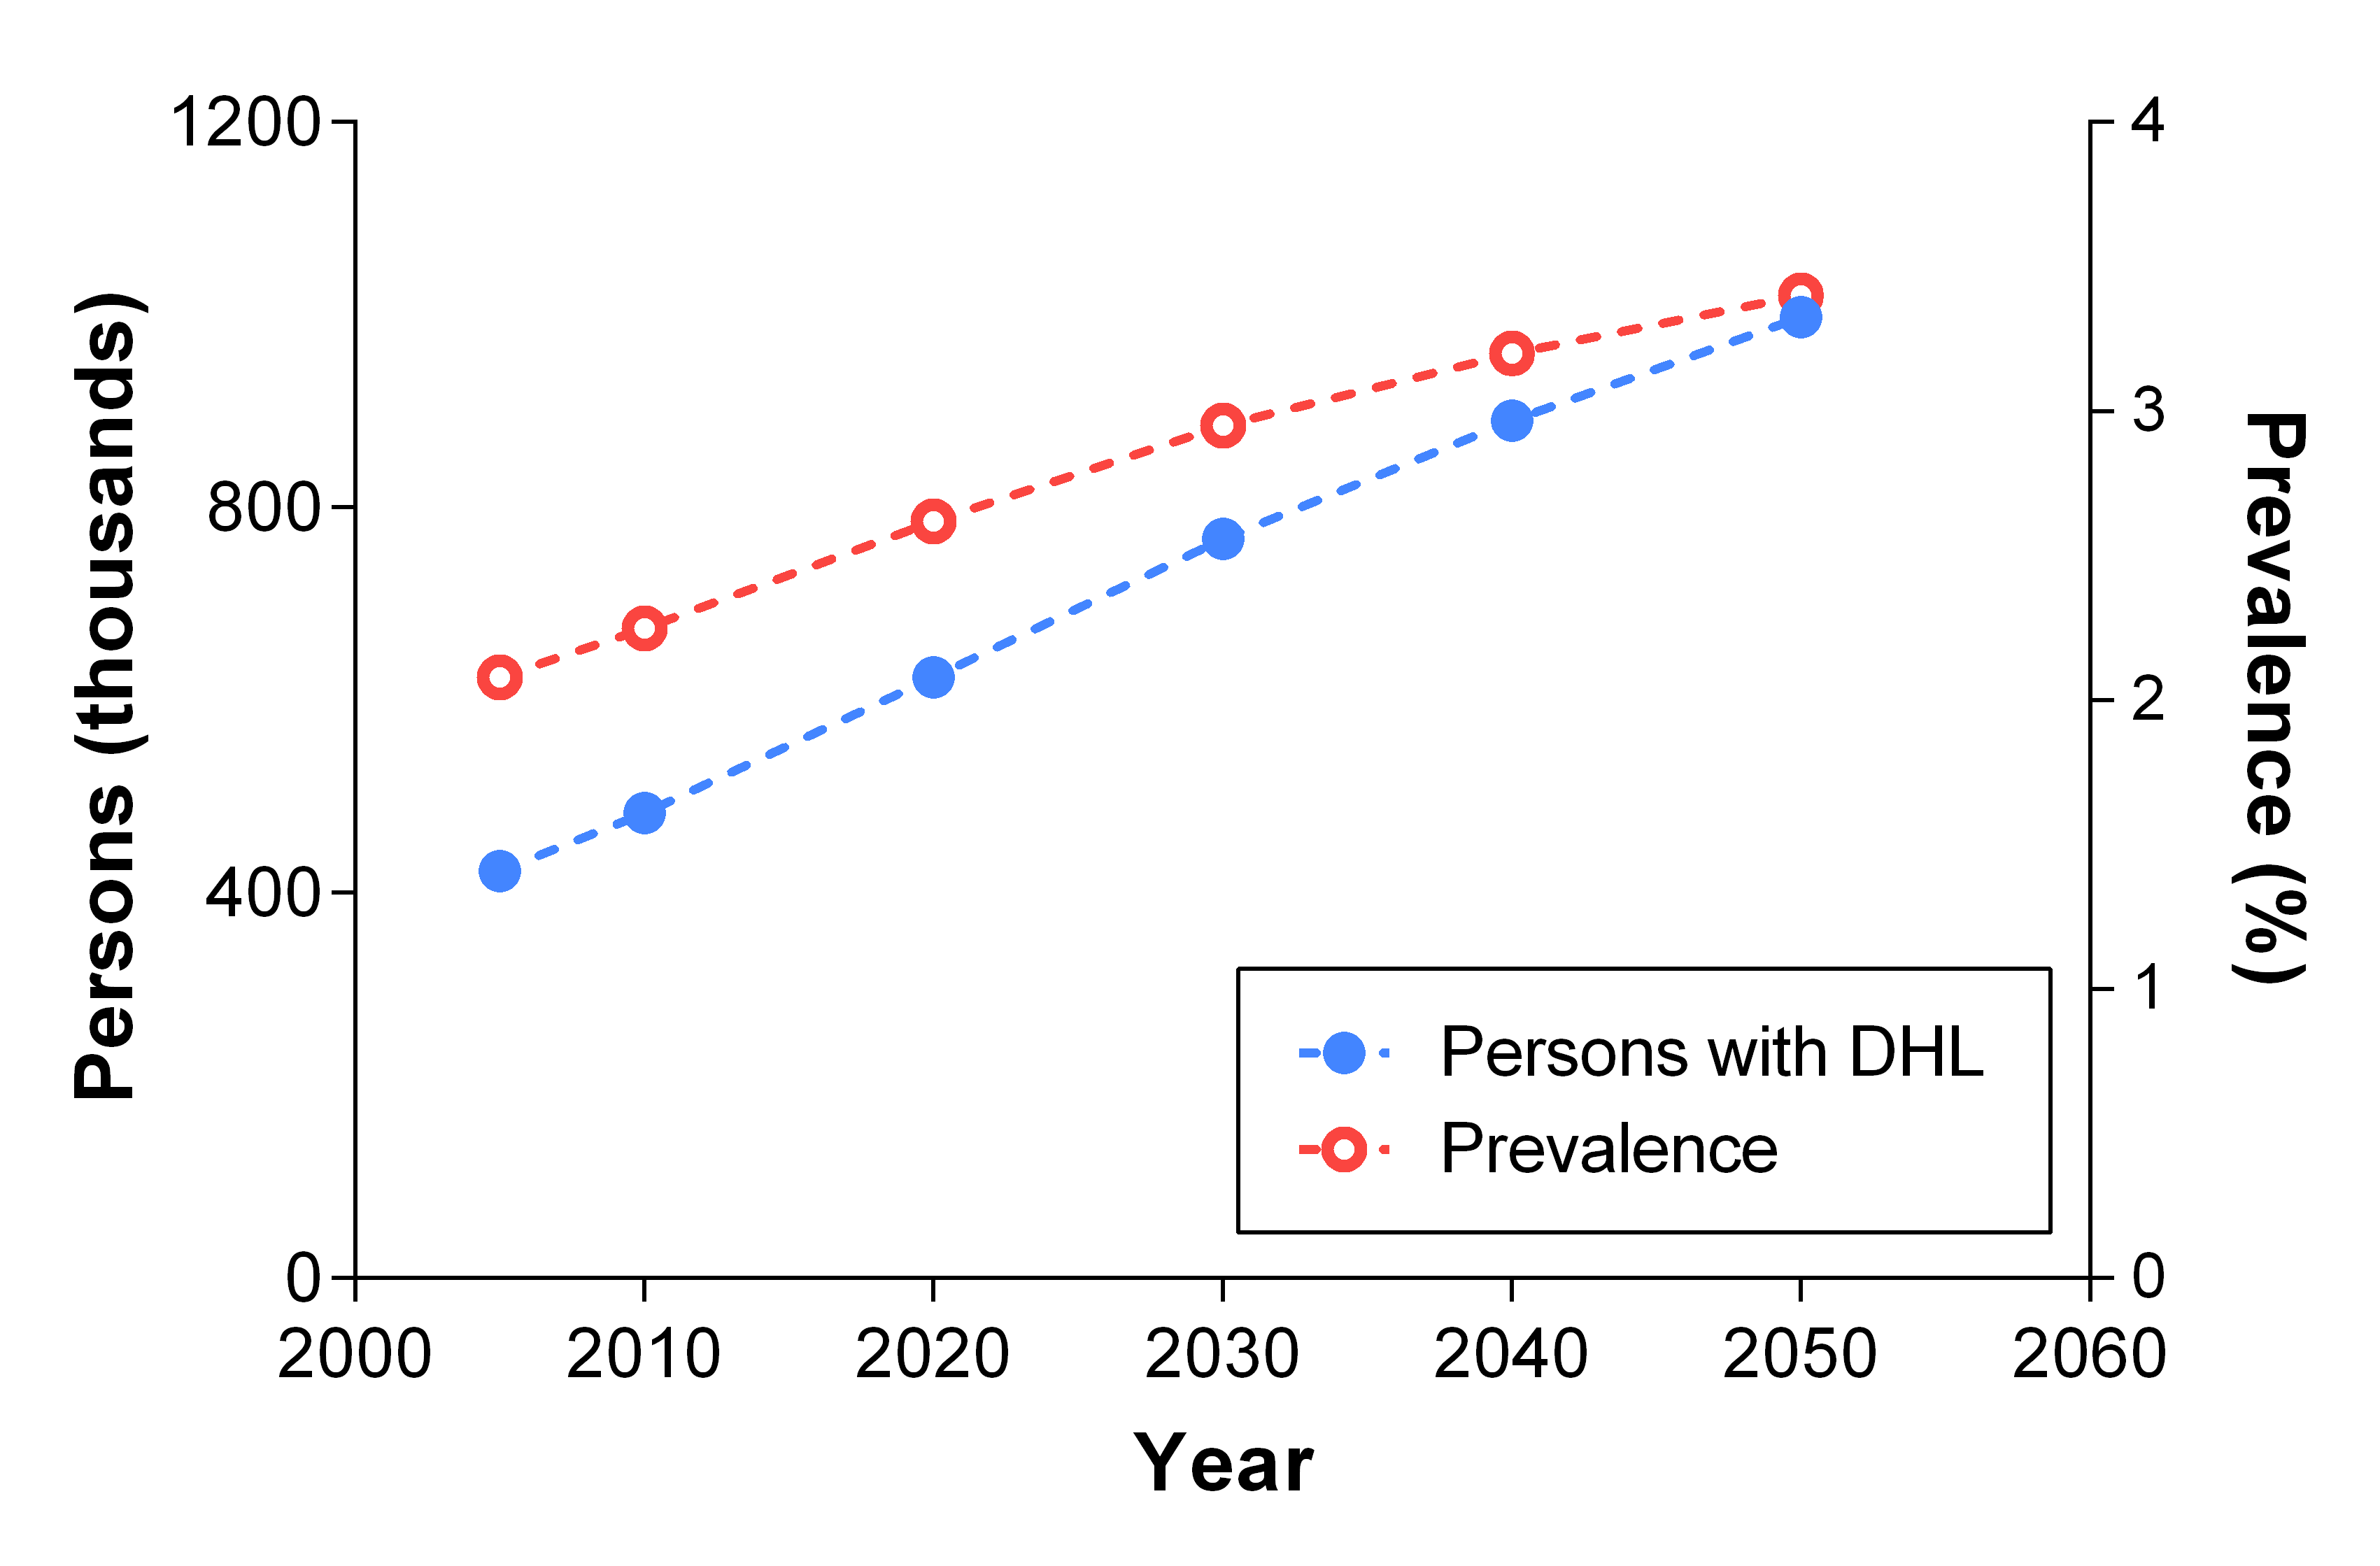
\includegraphics[height=8cm]{Introduction/hl_prevalence}
	\caption[Projected prevalence of disabling hearing loss in Australia]{Projected
	prevalence of disabling hearing loss (DHL) in Australia, 2005--2050. (Data from
	Access Economics~\cite{economics2006}.)}
	\label{fig:HL_prevalence}
\end{figure} 

Hearing loss comes with a number of personal costs to affected individuals in
addition to the reduced capacity to communicate. Quality of life is reduced
through suffering and loss of leisure~\cite{economics2006}. Participation in
education, skill development, and employment are hindered, putting pressure on
their consumable incomes which are, as a group, already lower than
average~\cite{economics2006}. Families, friends, and co-workers interacting with
the hearing impaired person are also affected, which can cause some individuals
to feel like they are a burden on those around them~\cite{mo2005}. Social
isolation is also well documented, and can lead to emotional tolls through
anxiety and depression~\cite{mo2005}.

The financial costs associated with hearing loss are
substantial~\cite{economics2006}. It was estimated to cost the Australian
economy about \$11.75 billion (1.4\% of gross domestic product) in 2005. The
largest component of this cost is productivity loss (\$6.7 billion), followed by
informal carers (\$3.2 billion), deadweight losses (\$1.0 billion), and then
direct health system costs (\$674 million). In addition to these numbers, the
monetary value corresponding to the loss of wellbeing described in the previous
paragraph was estimated to be some \$11.3 billion~\cite{economics2006}.

Considering the millions of people affected around the world, these Australian
estimates only represent a small fraction of the global total. It would appear
that the restoration of hearing capabilities would yield significant benefits
not only for affected individuals, but also for the economy as a whole. Indeed,
treatments for hearing loss are reportedly very cost-effective
interventions~\cite{economics2006}.

\subsection{The Cochlear Implant Performance Plateau}

Roughly 90\% of hearing loss is sensorineural in nature~\cite{wilson1998}, as
described in \S\ref{sect:hearing_loss}. For those categorised as having severe
or profound \emph{sensorineural hearing loss} (SHL), the cochlear implant (CI)
is the only effective treatment. Unlike hearing aids, which simply amplify
incoming sound signals, CIs work by injecting pulses of electric current into
the inner ear to stimulate auditory neurons directly
(\S\ref{sect:cochlear_implants}). The United States Food and Drug Administration
(FDA) reported that as of December 2012, approximately 324,200 people worldwide
had received CIs~\cite{nidcd2014}, and it is expected that this number will
continue to grow.

The quality of sound perception has shown marked improvements since CIs were
first developed. Figure~\ref{fig:sentence_recognition} shows the trend in
sentence recognition scores in quiet environments for CI recipients using
various sound processing strategies from the top device
manufacturers~\cite{zeng2008}. There were (and still are) significant variations
in speech performance amongst individuals~\cite{loizou1998}, but innovations in
the processing of speech signals~\cite{wilson1991nature,clark1996, loizou1998}
were able to produce rapid jumps in average performance over the first one and a
half to two decades of CI development.

\begin{figure}
	\centering
	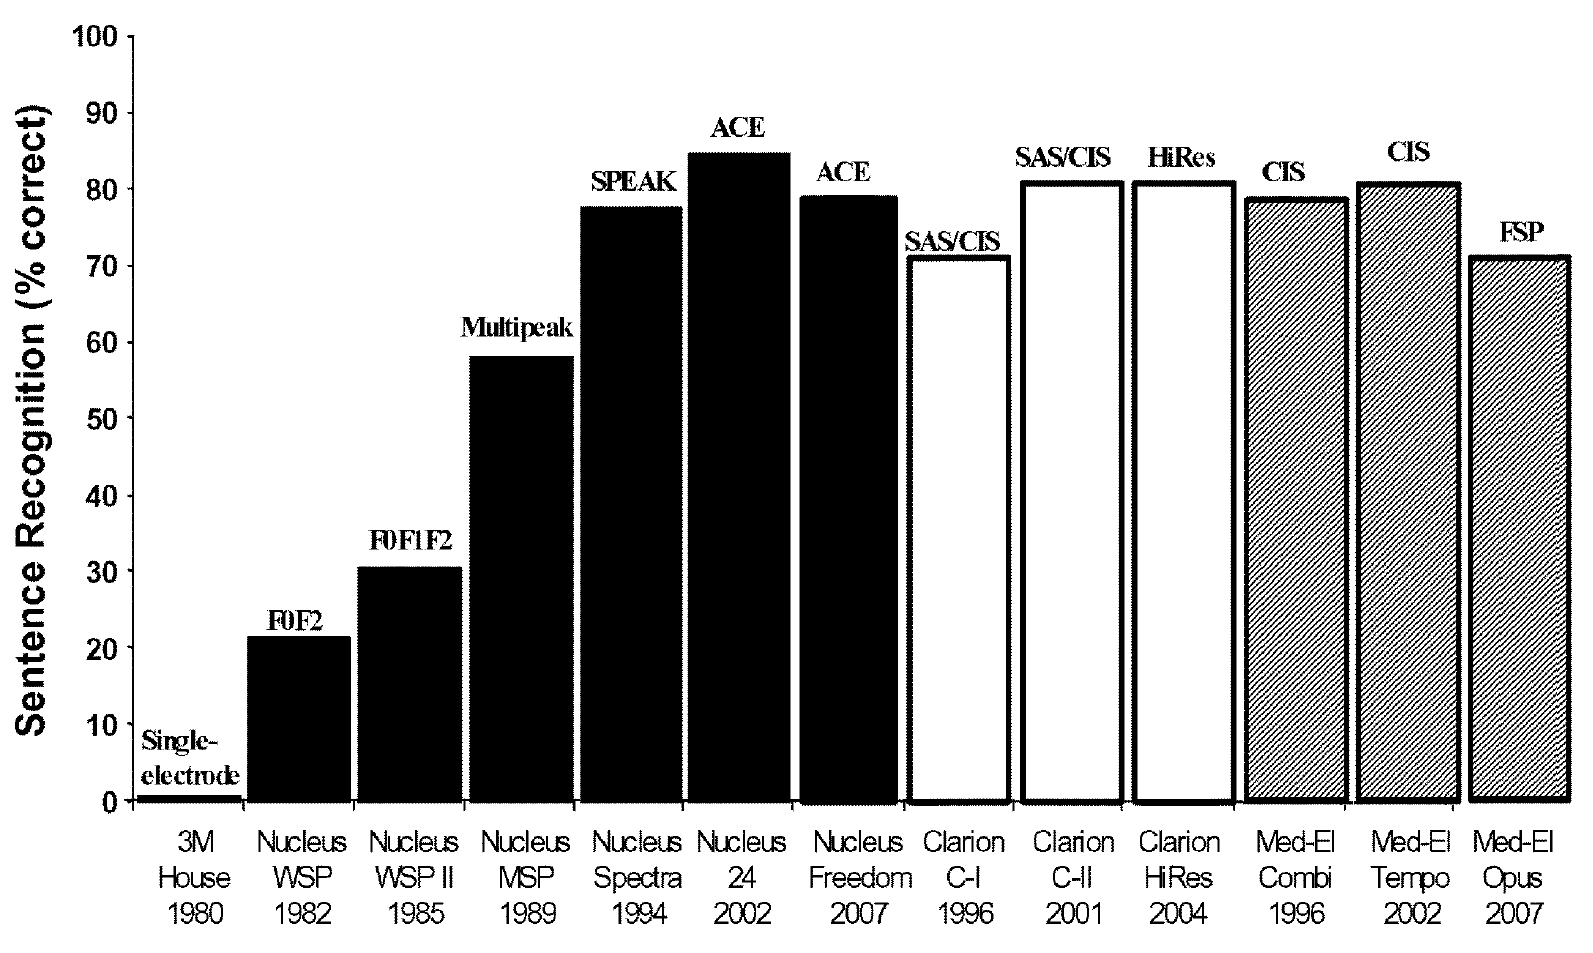
\includegraphics[height=8cm]{Introduction/sentence_recognition}
	\caption[Sentence recognition scores in quiet since 1980]{Sentence recognition
	scores in quiet since 1980. (Source: Zeng~\cite{zeng2008}. Copyright 
	\textcopyright{} 2008, IEEE.)}
	\label{fig:sentence_recognition}
\end{figure} 

Despite the technological merits of newer schemes, however, speech performance
in quiet has since plateaued~\cite{seligman2004,vandenhonert2007,zeng2008}. One
reason for this may be a shift in research focus towards improving other use
cases---with a large portion of users experiencing adequate performance in
quiet, researchers began working on performance in noisy environments, pitch
discrimination (for music and tonal languages), and other fringe cases to make
the implants more robust and relevant to the everyday lives of implant
recipients.

There may however be another potential explanation. Consider that the mechanism
ultimately responsible for hair cell stimulation is the \invivo{} current flow
(cf. \S\ref{sect:cochlear_implants}). The spatial distribution of this flow is
largely dictated by three factors: the design of the intracochlear electrode
array, its position within the cochlea after surgical insertion, and the
electrical properties of the tissues around the implant. The design of the array
is arguably the most important of these because it can affect both the
intrascalar positioning of the electrode array and, at least in part, the
surrounding tissue
response~\cite{miller1997,tykocinski2000,briggs2001,vanderbeek2005,
wardrop2005a,wardrop2005b,richardson2009}.

CI array designs have remained relatively stagnant in comparison to speech
processing techniques~\cite{girzon1987, micco2006, whiten2007}. This is not to
say that there has been zero progress in the area, but rather that the results
of such endeavours have failed to produce comparable successes. Part of the
reason for this may be a lack of impetus because early multichannel arrays were
more than sufficient to deliver the then-crude speech signals from the implant
electronics. Case in point, sentence recognition scores of over 90\% could be
obtained in quiet with just four active channels~\cite{shannon1995, dorman1997}.
As such, implants were designed with a 70 year life span [Cochlear Limited,
internal communication] in anticipation that software upgrades could be relied
on to improve performance.

With the sophistication of the latest algorithms corresponding to rather static
speech performance metrics, it would seem that the bottleneck has shifted to
other components of the system~\cite{clark2008,clark2013}. Whether these
limitations are due to array design or biological factors is not clear since the
influence of individual factors is difficult to ascertain~\cite{loizou1998}, but
it is most likely a combination of these. In either case, existing intracochlear
array designs have reached a limit, and a lack of insight into how they might
be further improved has hindered their continued development.

%% ================================================================== Objectives

\section{Thesis Goals}
\label{sect:thesis_goals}

\subsection{Enabling Knowledge Development via Computational Modelling}
\label{sect:knowledge_dev}

Traditional \invivo{} and \invitro{} methods for investigating biological
phenomena are difficult to implement in the cochlea because it is small,
contains a number of delicate structures, and is surgically inaccessible, being
encased in the densest and hardest bone in the body~\cite{bast1949, dallos1996}.
For the purposes of CI design, it is of interest to determine spatially
distributed field quantities~\cite{vanpoucke2004identification}. This presents
two main challenges to the experimentalist. Firstly, obtaining these
measurements using \invivo{} or \invitro{} methods can be impractical because
the probes must be physically placed at the location of the
measurements~\cite{girzon1987,kral1998}, a process which inherently compromises
the integrity of the cochlear structures. Most experiments therefore only
involve taking measurements within the fluid chambers of the cochlea, but even
then, introducing the probes requires perforation of either the otic capsule
surrounding the cochlea or the round window membrane and can damage the other
soft tissue structures lying within~\cite{black1980} or lead to cerebrospinal
fluid (CSF) contamination~\cite[p. 113]{salt1986}. Secondly, it is difficult to
precisely control the positioning of the probe to obtain the large number of
sample points needed for building a detailed electroanatomical map.

Over the past few decades, another method has become viable: computational
modelling, also referred to as \insilico{} experimentation. The progression of
``Moore's Law'', which predicts a doubling of the number of transistors in an
integrated circuit every two years~\cite{moore1998}, has led to a exponential
increase in processing power since the 1970s, enabling a range of numerical
methods (\S\ref{sect:numerical_methods}) to be adapted to engineering analysis.
Although the earliest \insilico{} studies were relatively simple abstractions,
the complexity of analyses that could be performed has increased over time,
spurred by the development of more robust software that took advantage of the
ever-increasing hardware capabilities.

A virtual representation of the implanted cochlea would be a useful tool for CI
research~\cite{girzon1987,micco2006,hanekom2015ciap} because it can provide an
alternative and complementary form of investigation that is not subject to the
shortcomings of traditional methods discussed above. Being able to manipulate a
virtual space means that measurements can be made in hard-to-reach places
(within Rosenthal's canal, for instance) without disturbing the surrounding
tissues, thereby providing a better representation of the \invivo{} situation.
In addition, more intuitive visualisations of the underlying bioelectric
phenomena can be produced, making the dissemination of new insights easier and
more accessible to a wider audience. When used in conjunction with \invivo{}
studies and bench-top testing, \insilico{} studies are invaluable for obtaining
a holistic understanding of medical
devices~\cite{kral1998,schimpf1998,fda2012,saba2012}.
To that end, the first goal of this project is \emph{to develop a realistic
computational model of the implanted cochlea}. All of the work that went into
producing the models in this thesis is documented in
Chapter~\ref{sect:modelling}.

Existing models of the implanted cochlea have a strong focus on explaining the
clinical outcomes observed in subjects, which is a significant and worthwhile
objective in itself, but in doing so they provide little insight into the
intermediate step of how injected current flows through the tissue both
spatially and temporally. This intermediate step must be understood in order to
gain insights that can be fed into the design process for next generation
intracochlear electrode arrays~\cite{girzon1987, schimpf1998}. It is hoped that
by analysing the relationships between the stimulating pulse, the anatomy of the
cochlea, and the electrophysiological response using computational techniques, a
more advanced understanding of the underlying mechanisms will be developed,
leading to improved intracochlear array designs that provide higher quality
sound perception, greater power efficiency, and other benefits to CI recipients.
To be clear, this is a longer term view for the industry. The focus for this
project is to develop the groundwork, methodology, and models that would enable
this future to take place.

\subsection{Addressing Untested Assumptions in the Literature}

Consider the following quote from statistician George Box: 

\begin{verse}

	\textit{
		``Essentially, all models are wrong, but some are useful. \hphantom{This is
		some filler text} \ldots the approximate nature of the model must always be
		borne in mind.'' }

 	\vspace{4mm}
	\raggedleft{
		--- George Box, 1987~\cite{box1987}
	}
\end{verse}

All models are, by definition, simplifications of reality. Sophisticated models
may approach the reality of nature, but they will never replicate it entirely;
nor should they, given that the purpose of modelling is to make complexity more
intuitive [Lianne Cartee, personal communication]. For practical purposes, what
matters is whether or not they are representative of the system being studied.

Simply creating a model does not provide an adequate foundation for further
investigation. As noted in \S\ref{sect:validation_intro}, there is some
entrenched reluctance to trust computational models in the CI research
community, despite the benefits and insights that they can provide. It is
suspected that this is due to the use of untested assumptions in existing models
that are often not intuitive nor properly justified. Coupled with the
inconsistent predictions of psychophysical outcomes from one model to the next,
which are inevitable given the multiple layers of abstraction and the difficulty
of representing biophysical interactions mathematically, it is understandable
that these doubts exist.

Hence, the second goal of this project is \emph{to critically evaluate some of
the assumptions currently used in volume conduction models of the cochlea}.
These include the impact of boundary conditions
(Chapters~\ref{sect:boundary_conditions} and \ref{sect:validation}), material
properties (Chapter~\ref{sect:validation}), vascular structure
(Chapter~\ref{sect:vascular_structure}), and time-dependent effects
(Chapter~\ref{sect:time_dependency}). Sensitivity studies will be performed to
gauge the certainty of cited input parameters, and \invivo{} measurements will
be acquired and compared with the \insilico{} results to provide guidance on
acceptable model outputs. By addressing these outstanding issues in a thorough
and logical manner, it is hoped that some of the concerns surrounding the use of
\insilico{} models may be alleviated. The outcome of these assessments will act
to either further validate existing models, or prompt changes in future models.
In either case, the profile and trustworthiness of computational models of the
implanted cochlea will be improved.


% On the other hand, the approach is also subject to several limitations <list
% cons --- realism, material properties of anisotropic biological tissues>.
% ~\cite{martini2006,johnson2006}

% Still problems to be overcome in bioelectric modelling: Potratz
% paper?~\cite{potratz2010}

% The complexity of human anatomy is further compounded by the variability between
% individuals \cite{lau2011}; this is true also for the cochlea, which despite
% being one of the smallest organs in the human body still exhibits significant
% disparities \cite{axelsson1968}

%% ========================================================== Document Structure

\section{Dissertation Structure}

The structure of the dissertation is as follows:

\begin{description}
	\item[\textsf{Chapter 1}] Explains the motivation behind the project and the
	goals of the thesis.
	\item[\textsf{Chapter 2}] Reviews the anatomy of the ear and the processes
	responsible for hearing.
	\item[\textsf{Chapter 3}] Introduces cochlear implants, examines existing work
	in bioelectric modelling to develop the reader's knowledge of the subject
	matter, and reviews the current state-of-the-art.
	\item[\textsf{Chapter 4}] Documents the methodology used to construct the
	models in the thesis.
	\item[\textsf{Chapter 5}] Examines the impact and accuracy of various
	boundary condition assumptions.
	\item[\textsf{Chapter 6}] Assesses the validity of the guinea pig cochlea model
	to ensure that input parameters and corresponding results are reasonable.
	\item[\textsf{Chapter 7}] Investigates the role of vascular	structures in
	volume conduction.
	\item[\textsf{Chapter 8}] Evaluates the feasibility of modelling
	time-dependent effects and the repercussions of these dynamics.
	\item[\textsf{Chapter 9}] Summarises the findings of the thesis and proposes
	directions for future research efforts.
\end{description}
			% Chapter 1: Introduction
	% Page style for this chapter
	\pagestyle{fancy}
	\lhead{{\sffamily \MakeUppercase{2. The Peripheral Auditory System}}}
	\chead{}
	\rhead{{\sffamily \MakeUppercase\rightmark}}
	\lfoot{}
	\cfoot{{\sffamily \thepage}}
	\rfoot{}
	
\chapter{Anatomy and Physiology of the Peripheral Auditory System}

% Textbox
\begin{center}
	\begin{tcolorbox}[title=\boxtitle]
		\begin{itemize}[leftmargin=*,labelindent=2ex,labelsep=1.5ex,itemsep=0pt,parsep=0pt]
		    \item What structures are involved in hearing perception?
    		\item What does the cochlea look like?
			\item How does normal hearing work?
		\end{itemize}
	\end{tcolorbox}
\end{center}

%% ============================================================== Anatomy Review

\section{Anatomy Review}
\label{sect:anatomy_review}

\subsection{Overview of the Auditory Pathway}

The ability to hear involves a chain of anatomical structures that together form
the auditory pathway. It includes the various components of the ear, which are
responsible for the detection and encoding of sound stimuli, the neural pathways
that relay the encoded neural signal to the brain, and the auditory cortex, the
part of the brain that processes and interprets the received
signal~\cite{goldstein2009}.

The ear can be divided into three distinct regions: the external ear, the middle
ear, and the inner ear, as illustrated in Figure~\ref{fig:ear_overview}. Each
region is described briefly below.

\subsubsection{The External Ear}

The purpose of the external ear is to collect and direct sound waves towards the
middle ear. This is primarily facilitated by the \emph{auricle}, a cartilaginous
structure making up the portion of the ear visible from outside the body. Its
shape helps to funnel sound waves into the \emph{external acoustic meatus}, a
narrow tunnel that passes through the temporal bone of the skull. At the medial
end of the meatus is a thin sheet of connective tissue called the \emph{tympanic
membrane}, commonly known as the eardrum.

\begin{figure}[p]
	\centering
	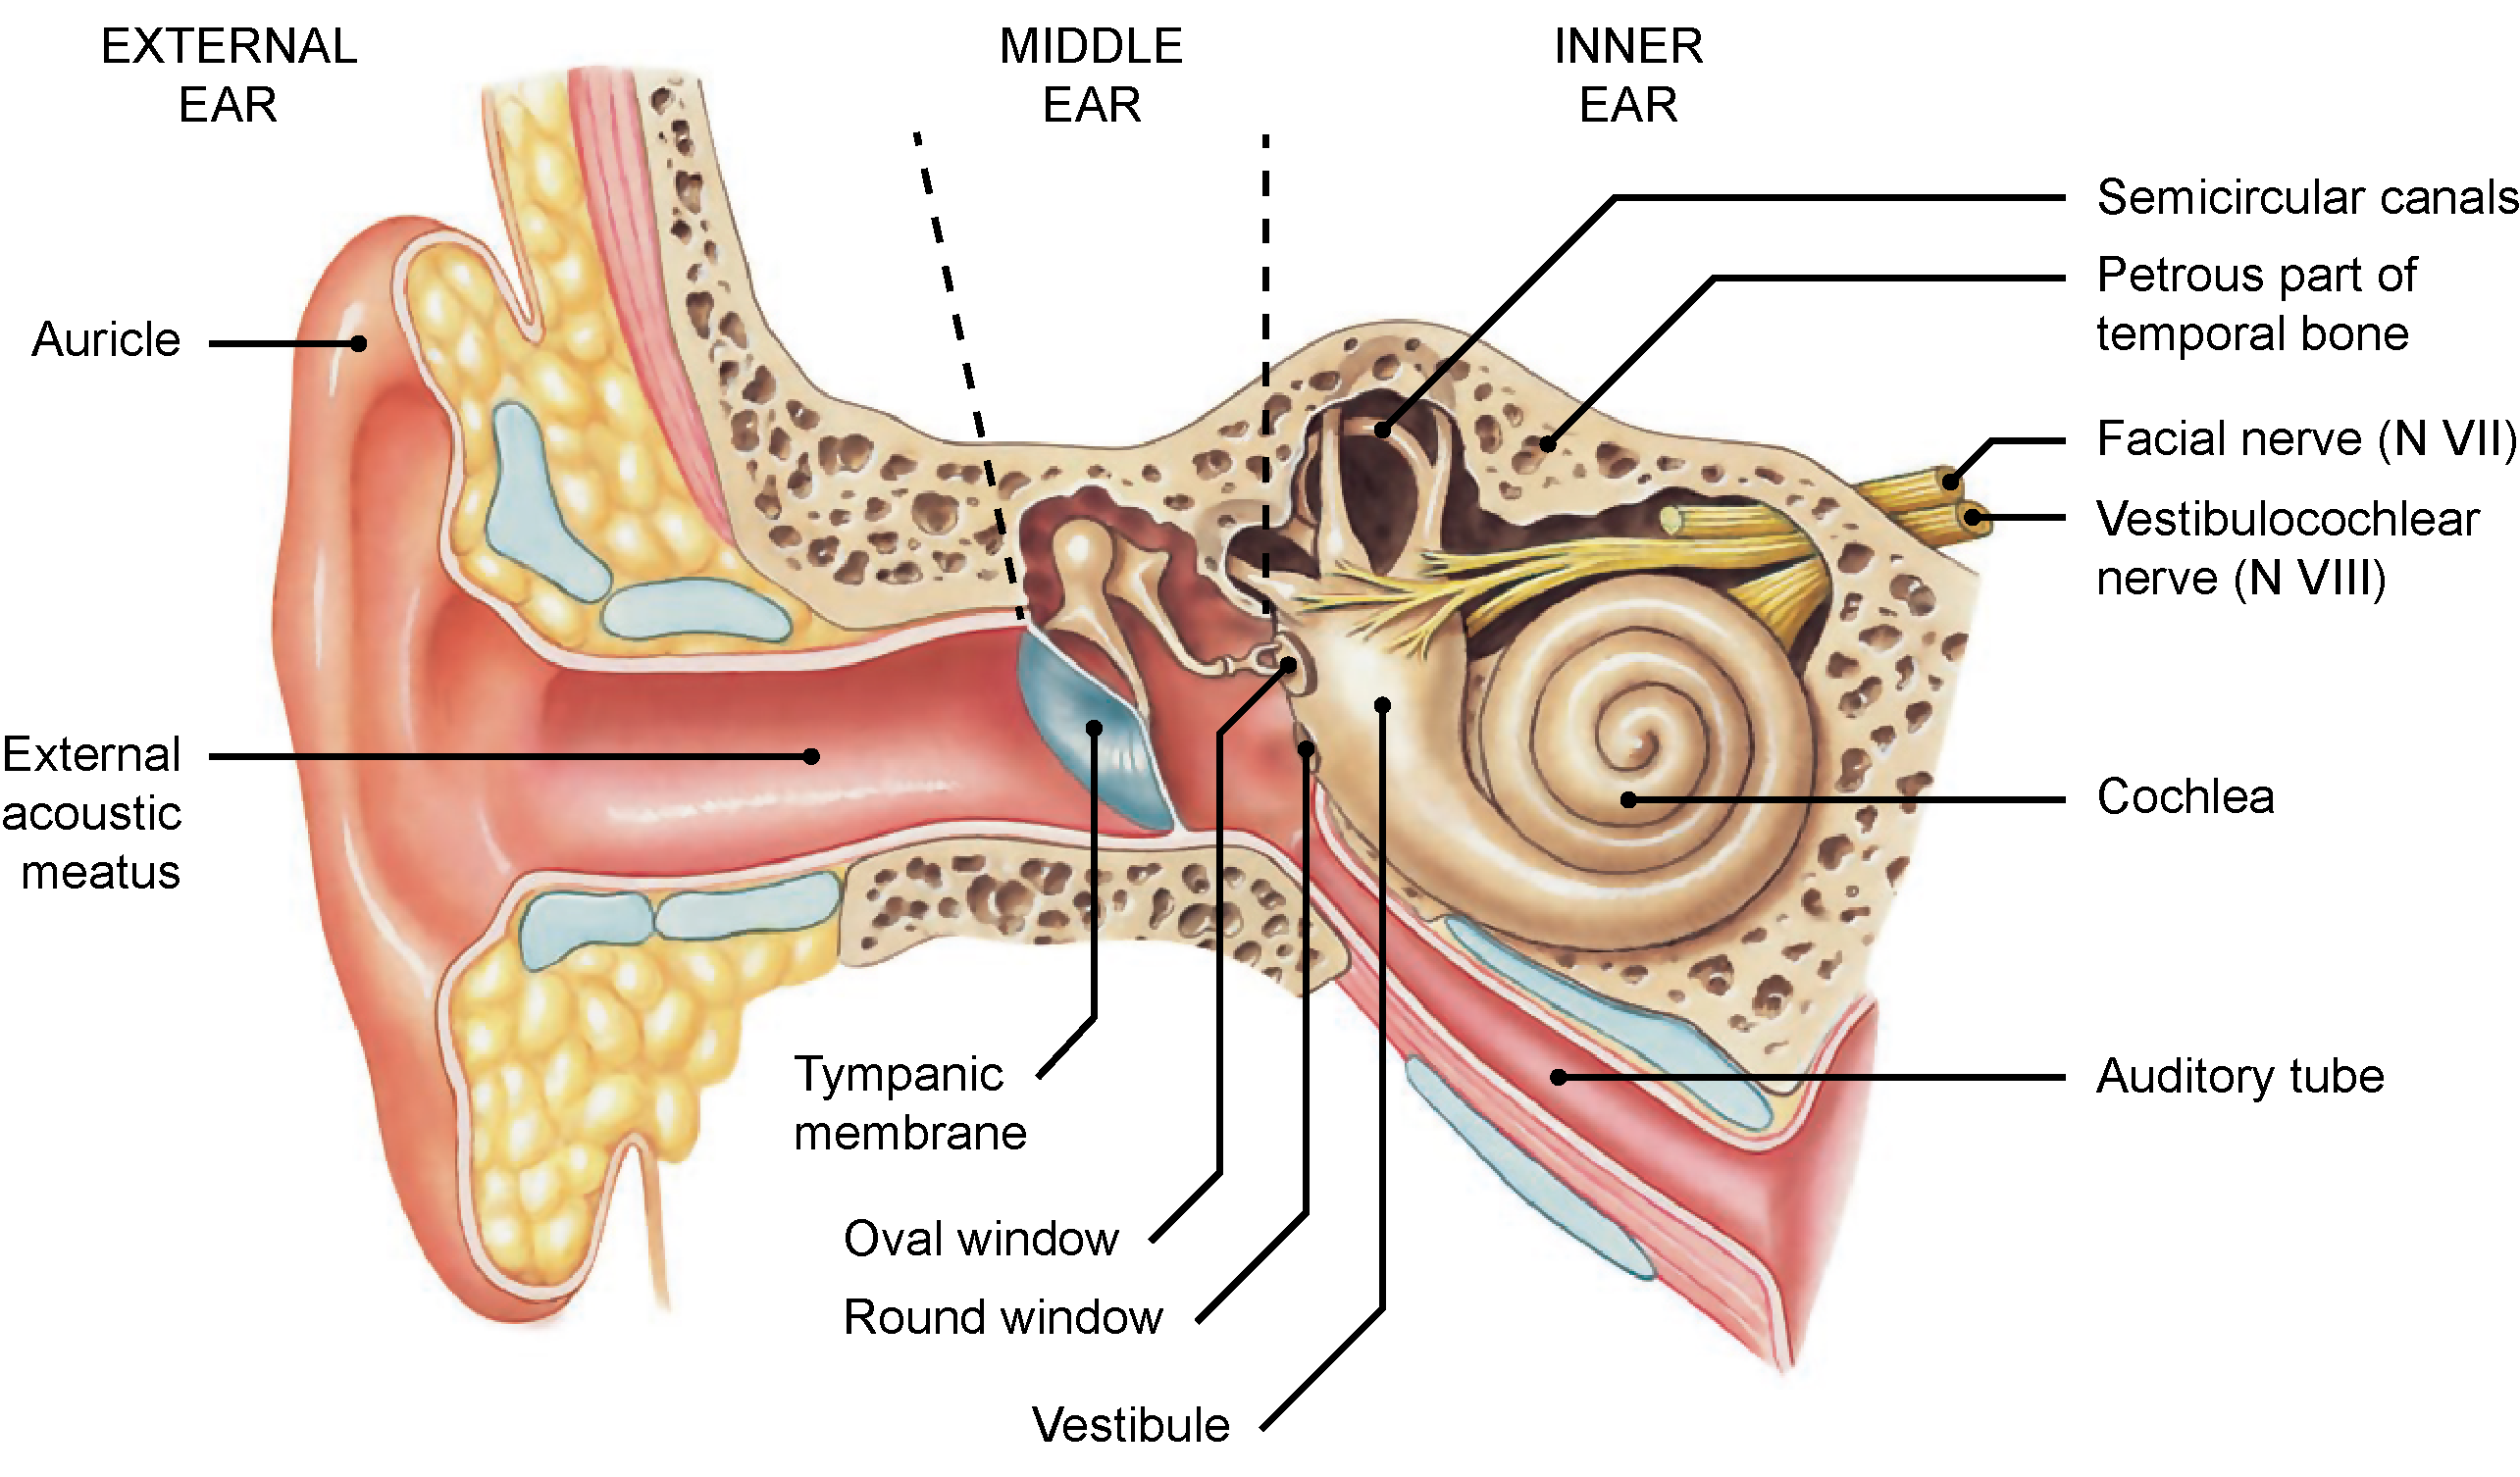
\includegraphics[width=\textwidth]{Background/ear_labelled.pdf}
	\caption[The anatomy of the ear]{The anatomy of the ear. (Image adapted from
	Martini~\etal~\cite{martini2006}. Copyright \textcopyright{} 2006, Daryl Fox.)}
	\label{fig:ear_overview}
\end{figure}

\begin{figure}[p]
	\centering
	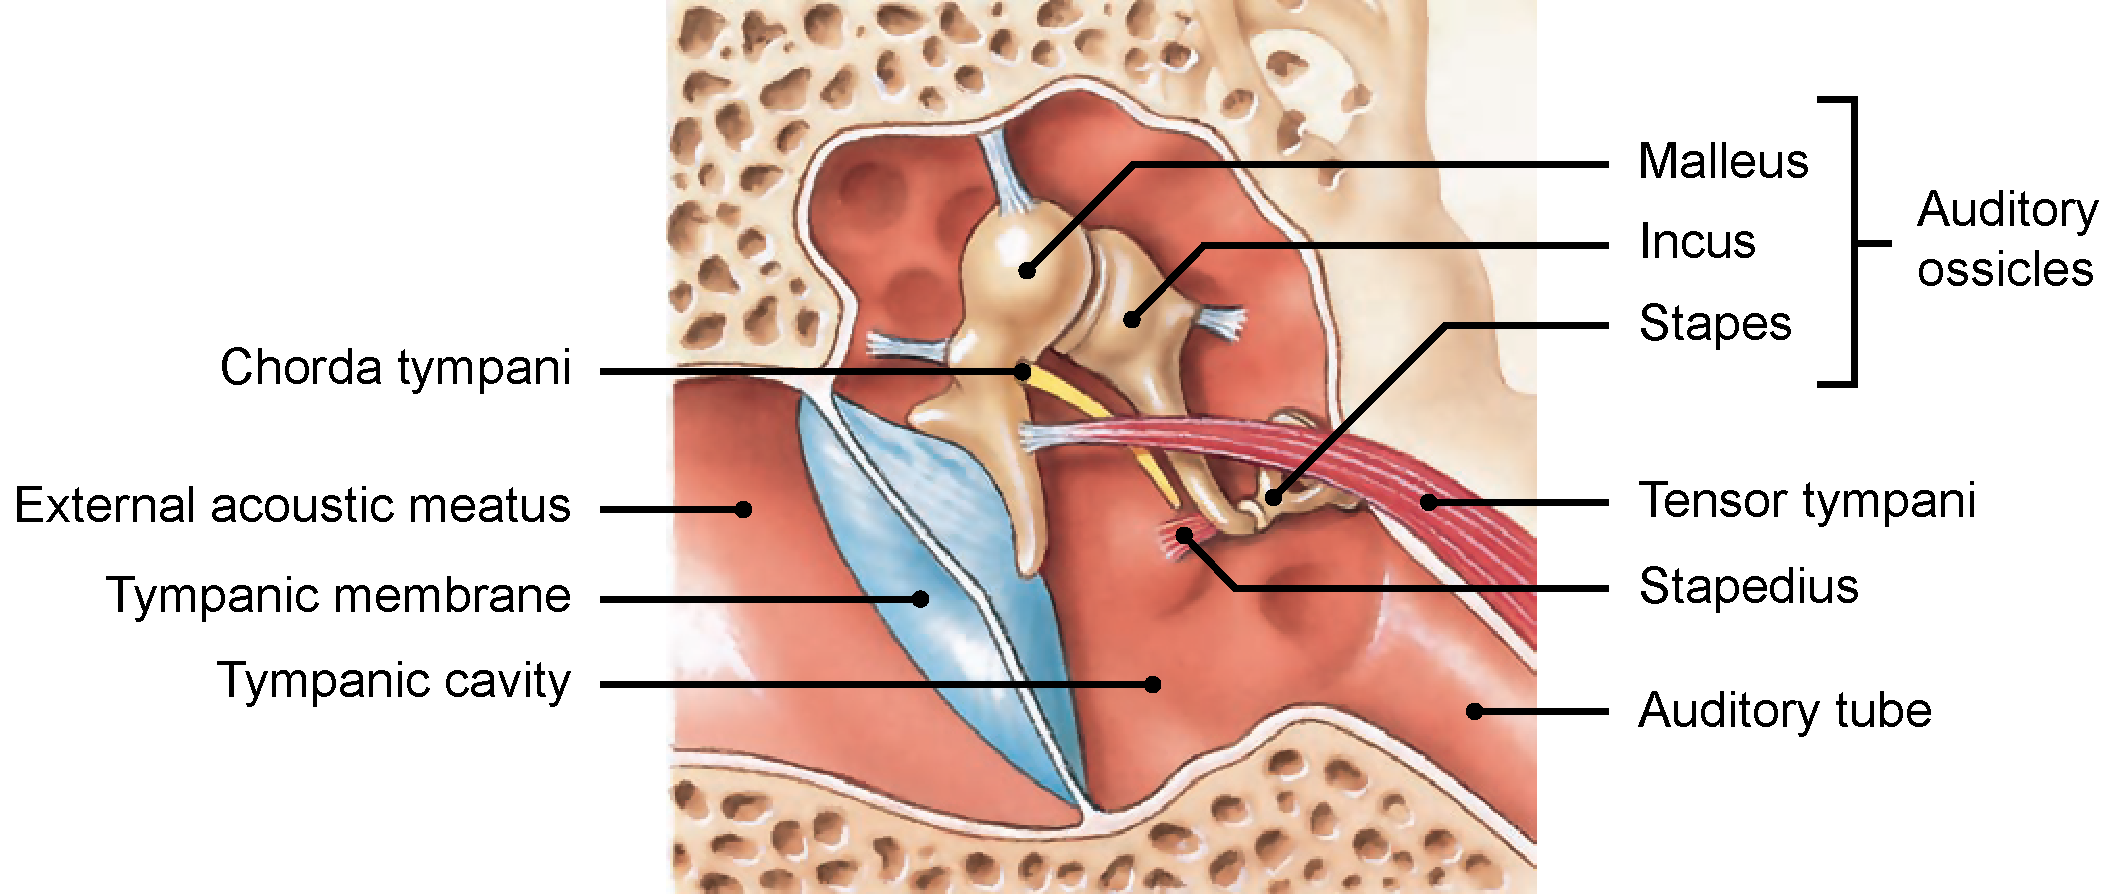
\includegraphics[width=13.3cm]{Background/middle_ear_labelled.pdf}
	\caption[Structures within the tympanic cavity]{Structures within the
	tympanic cavity. (Image adapted from Martini~\etal~\cite{martini2006}.
	Copyright \textcopyright{} 2006, Daryl Fox.)}
	\label{fig:middle_ear}
\end{figure}

\subsubsection{The Middle Ear}

On the other side of the tympanic membrane is a small, air-filled chamber called
the \emph{tympanic cavity} (see Figure~\ref{fig:middle_ear}). It opens
inferiorly into the \emph{auditory tube}, which leads to the nasopharynx. This
connection allows the air pressure on both the sides of the tympanic membrane to
be maintained at the external atmospheric pressure.

The key feature of the middle ear is its three tiny bones---the \emph{malleus},
the \emph{incus}, and the \emph{stapes}---collectively known as the
\emph{auditory ossicles}. The malleus is attached to the tympanic membrane
inferiorly and to the incus superiorly; in turn, the incus is linked to the
stapes, whose footplate is fused to an opening in the bony wall of the inner ear
known as the \emph{oval window} (see Figure~\ref{fig:ear_overview}). The
ossicles conduct and amplify the vibrations of incoming sound waves from the
tympanic membrane through the oval window to the inner ear.

Three other structures located in the middle ear are the \emph{tensor tympani}
and \emph{stapedius} muscles, and the \emph{chorda tympani} nerve. The muscles
prevent excessive movement of the tympanic membrane and ossicles that would
otherwise damage these delicate structures. The nerve carries taste sensations,
and passes through the tympanic cavity to join with the nearby \emph{facial
nerve} (or seventh cranial nerve, N~VII).

\subsubsection{The Inner Ear}

Sensory receptors for both hearing and equilibrium are housed in the chambers of
the inner ear (Figure~\ref{fig:inner_ear}). The \emph{membranous labyrinth},
which contains a fluid called \emph{endolymph}, is surrounded by the \emph{bony
labyrinth} (also known as the \emph{otic capsule}~\cite[p. 62]{jahn2001}), and
the space between them is filled with another fluid called \emph{perilymph}.
Endolymph and perilymph are both extracellular fluids but they have different
compositions, as shown in Table~\ref{table:fluid_composition}. The high
potassium concentration of endolymph is required for normal hearing function and makes it
unique amongst bodily fluids. The composition of perilymph is similar to that of
cerebrospinal fluid (CSF), likely because they are joined via the
\emph{perilymphatic duct}. There are subtle variations in composition between
the two perilymphatic fluid chambers, with only the amount of protein showing a
large discrepancy.

\begin{figure}
	\centering
	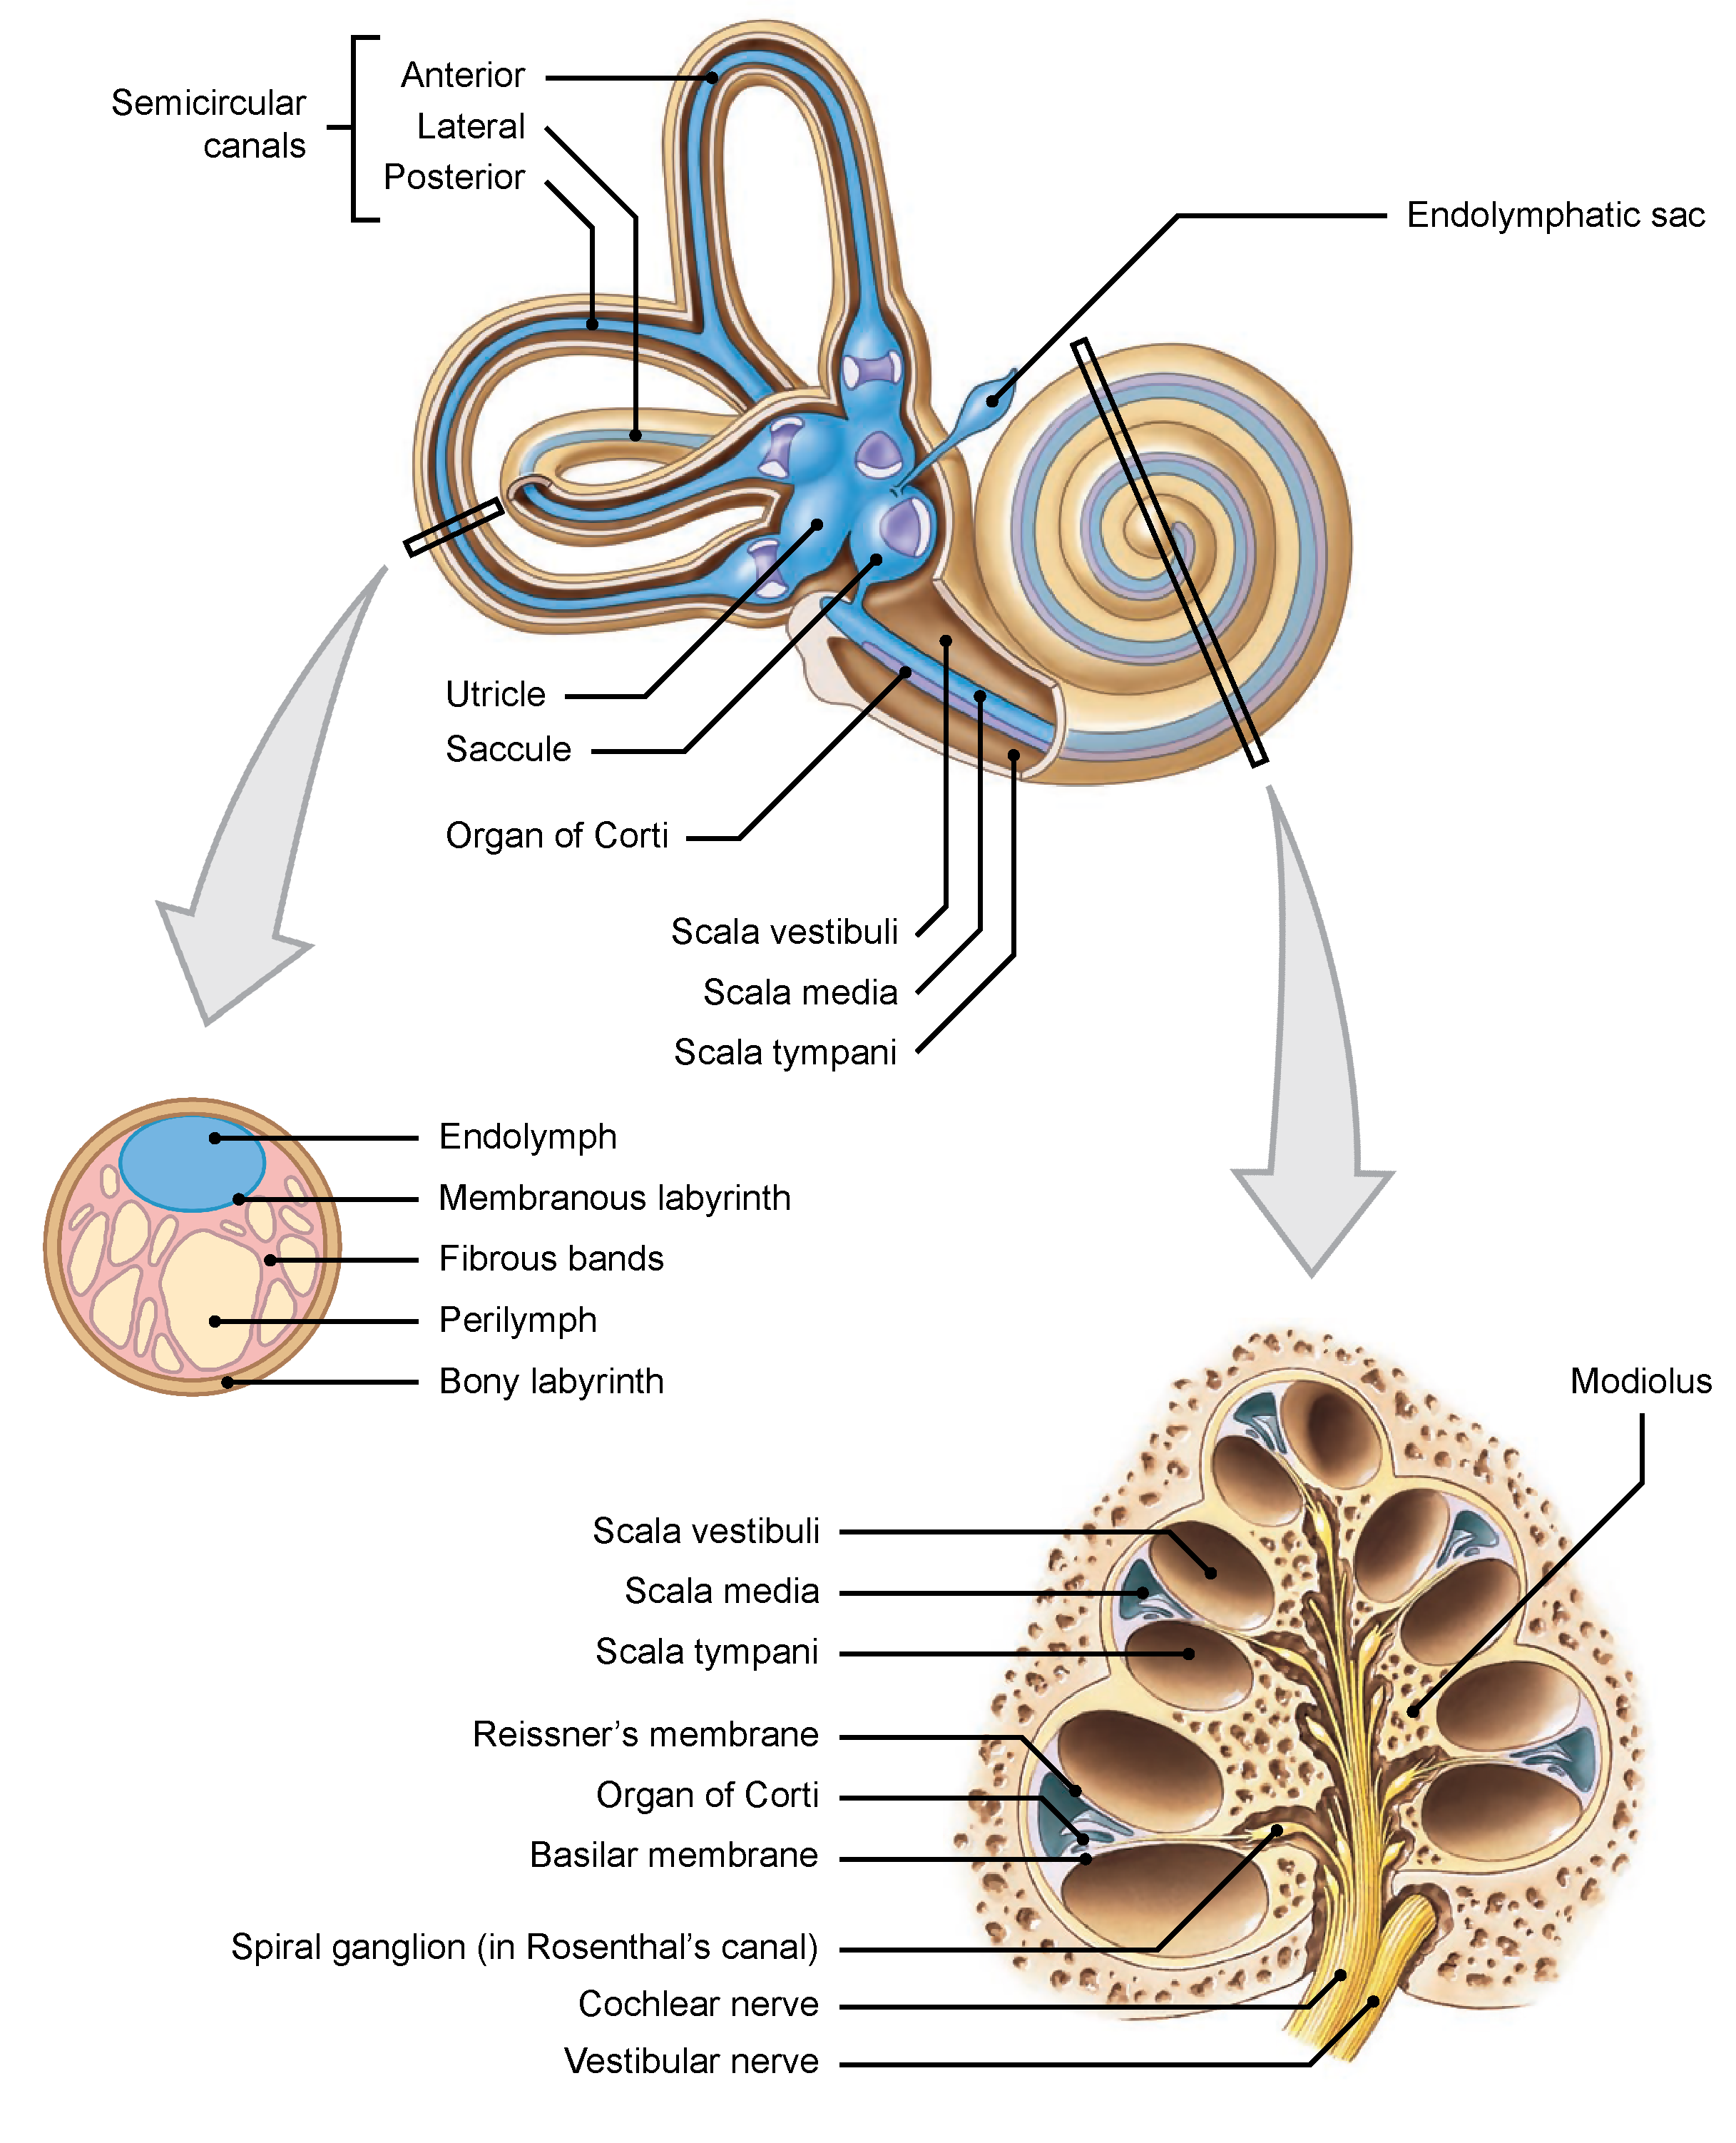
\includegraphics[width=\textwidth]{Background/labyrinths_labelled_ext.pdf}
	\caption[Labyrinths of the inner ear]{Labyrinths of the inner ear. (Image
	adapted from Martini~\etal~\cite{martini2006}. Copyright \textcopyright{} 2006,
	Daryl Fox.)}
	\label{fig:inner_ear}
\end{figure}

\begin{table}
	\centering
	\sffamily
	\small
	\caption[Composition of the inner ear fluids]{Composition of the inner ear
	fluids. All values are reported in millimolar (mM), except for protein.
	Measurements were obtained from various studies on guinea pigs and rodents. Not
	all constituents have been listed. (Data from Wangemann and
	Schacht~\cite{wangemann1996}.)}
	\label{table:fluid_composition}
	
	\begin{tabular}{l c c c c}
		\toprule
		\textbf{Component}	& \textbf{Endolymph of}	& \textbf{Perilymph of}	
			& \textbf{Perilymph of}		& \textbf{Cerebrospinal} \\
							& \textbf{scala media}	& \textbf{scala vestibuli}
			& \textbf{scala tympani}	& \textbf{fluid} \\
		\midrule
		
		\csvreader[late after line=\\]%
			{Background/fluid_compositions.csv}%
			{Component=\comp,Endolymph (SM)=\esm,Perilymph (SV)=\psv,Perilymph (ST)=\pst,CSF=\csf}%
 			{\comp & \esm & \psv & \pst & \csf}%
		\bottomrule
	\end{tabular}
	
\end{table}

The posterolateral aspects of the inner ear, namely the \emph{vestibule} (see
Figure~\ref{fig:ear_overview}) and the semicircular canals, together form the
\emph{vestibular complex}. Sensations of gravity, linear acceleration and head
rotation all arise from the receptors in this region. The sensation of hearing
occurs in the anteromedial aspect, which is named the \emph{cochlea} after its
distinctive snail shell appearance. For both of these senses, the reception of
stimuli and their transduction into neuronal signals is handled by highly
specialised mechanoreceptors called \emph{hair cells} (see inset,
Figure~\ref{fig:corti}).

The structure of the cochlea is described in more depth in
\S\ref{section:cochlea_detail}.

\subsubsection{Neural Pathways to the Auditory Cortex}
\label{section:neural_pathways}

Hair cells are monitored by the peripheral nerve endings of auditory neurons.
The cell bodies of these predominantly bipolar neurons are unmyelinated in
humans~\cite{ota1980} and are clustered together in the \emph{spiral ganglion},
housed within \emph{Rosenthal's canal} (see Figure~\ref{fig:inner_ear}). Their
myelinated axons combine to form the \emph{cochlear nerve}, which exits the
cochlea via its basal end and joins with the \emph{vestibular nerve} exiting the
vestibular complex to become the \emph{vestibulocochlear nerve}, also known as
the auditory nerve (or eighth cranial nerve, N~VIII). These branches, shown in
Figure~\ref{fig:tonotopy}, follow the \emph{internal auditory meatus} through
the petrous part of the temporal bone and are encased in CSF.

\begin{figure}
	\centering
	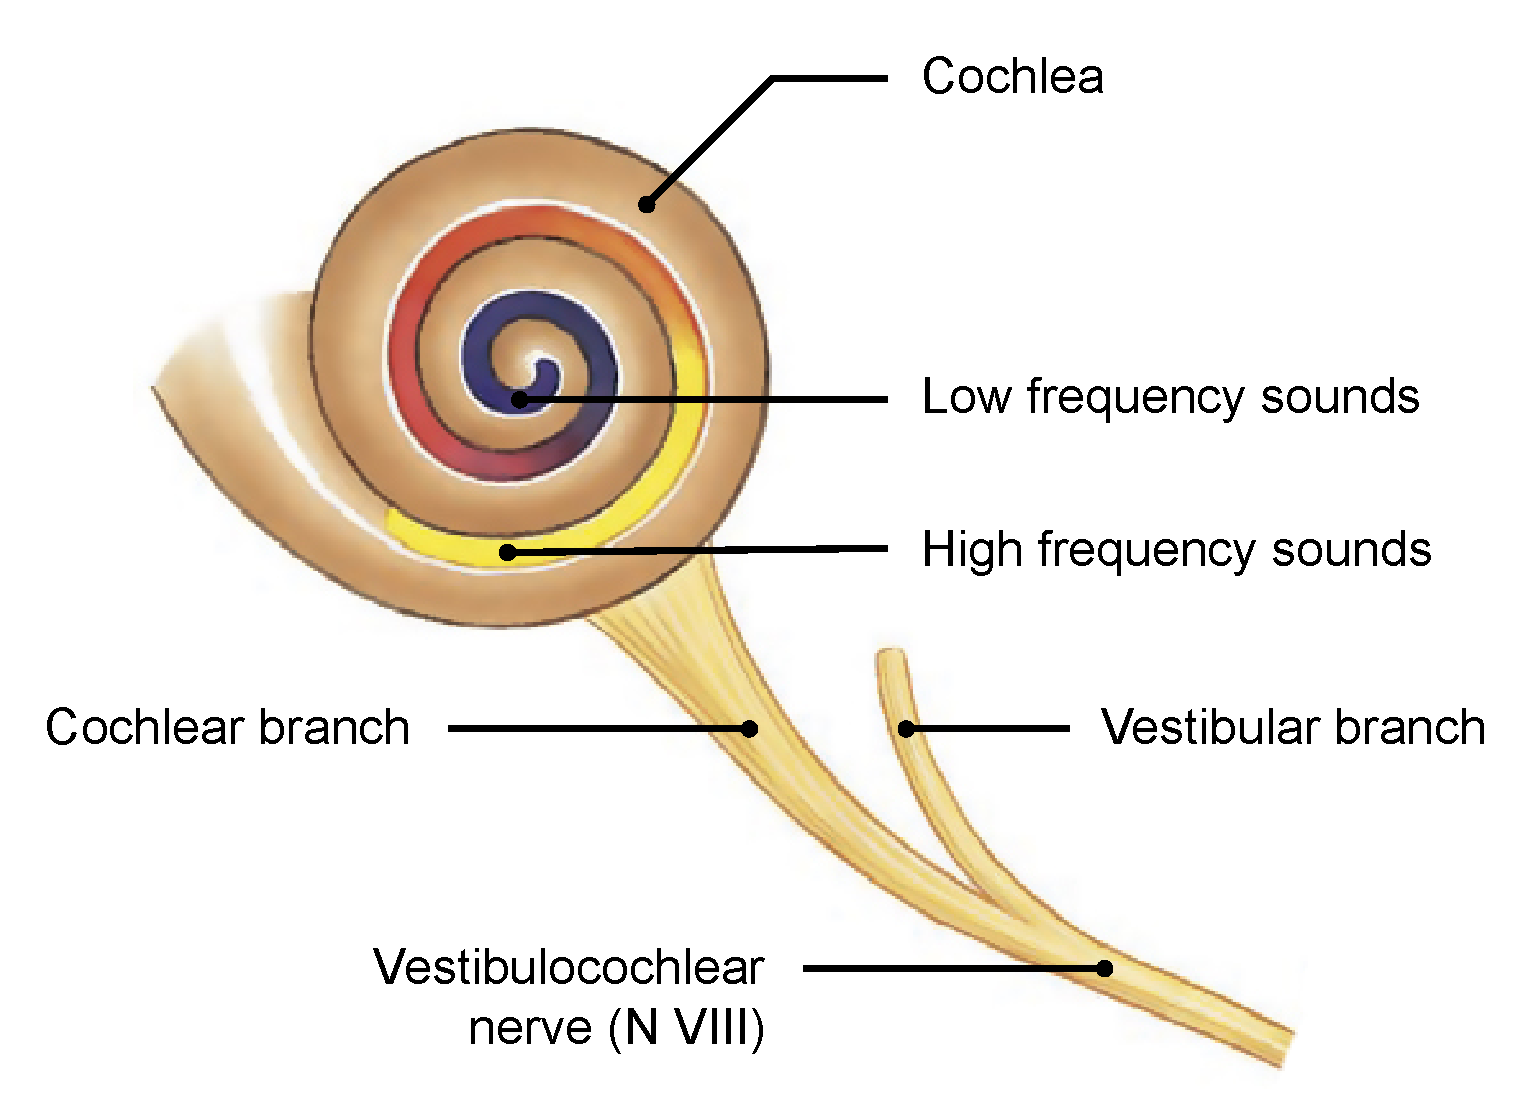
\includegraphics[width=9.8cm]{Background/tonotopy}
	\caption[Tonotopic organisation of the cochlea]{Tonotopic organisation of the
	cochlea. Low and high frequency receptors join together to form the cochlear
	branch of N VIII. The sequential frequency mapping is preserved and
	transferred to the auditory cortex (cf. Figure~\ref{fig:auditory_cortex}).
	(Image adapted from Martini~\etal~\cite{martini2006}. Copyright
	\textcopyright{} 2006, Daryl Fox.)}
	\label{fig:tonotopy}
\end{figure}

Upon reaching the ipsilateral \emph{cochlear nucleus} in the medulla oblongata,
second-order neurons decussate and ascend to the \emph{inferior colliculus},
which is responsible for auditory reflexes. Connecting neurons propagate the
signal to the \emph{medial geniculate nucleus} in the thalamus, before finally
reaching the \emph{auditory cortex} in the temporal lobe of the brain. These
pathways are illustrated in Figure~\ref{fig:auditory_cortex}.

\begin{figure}
	\centering
	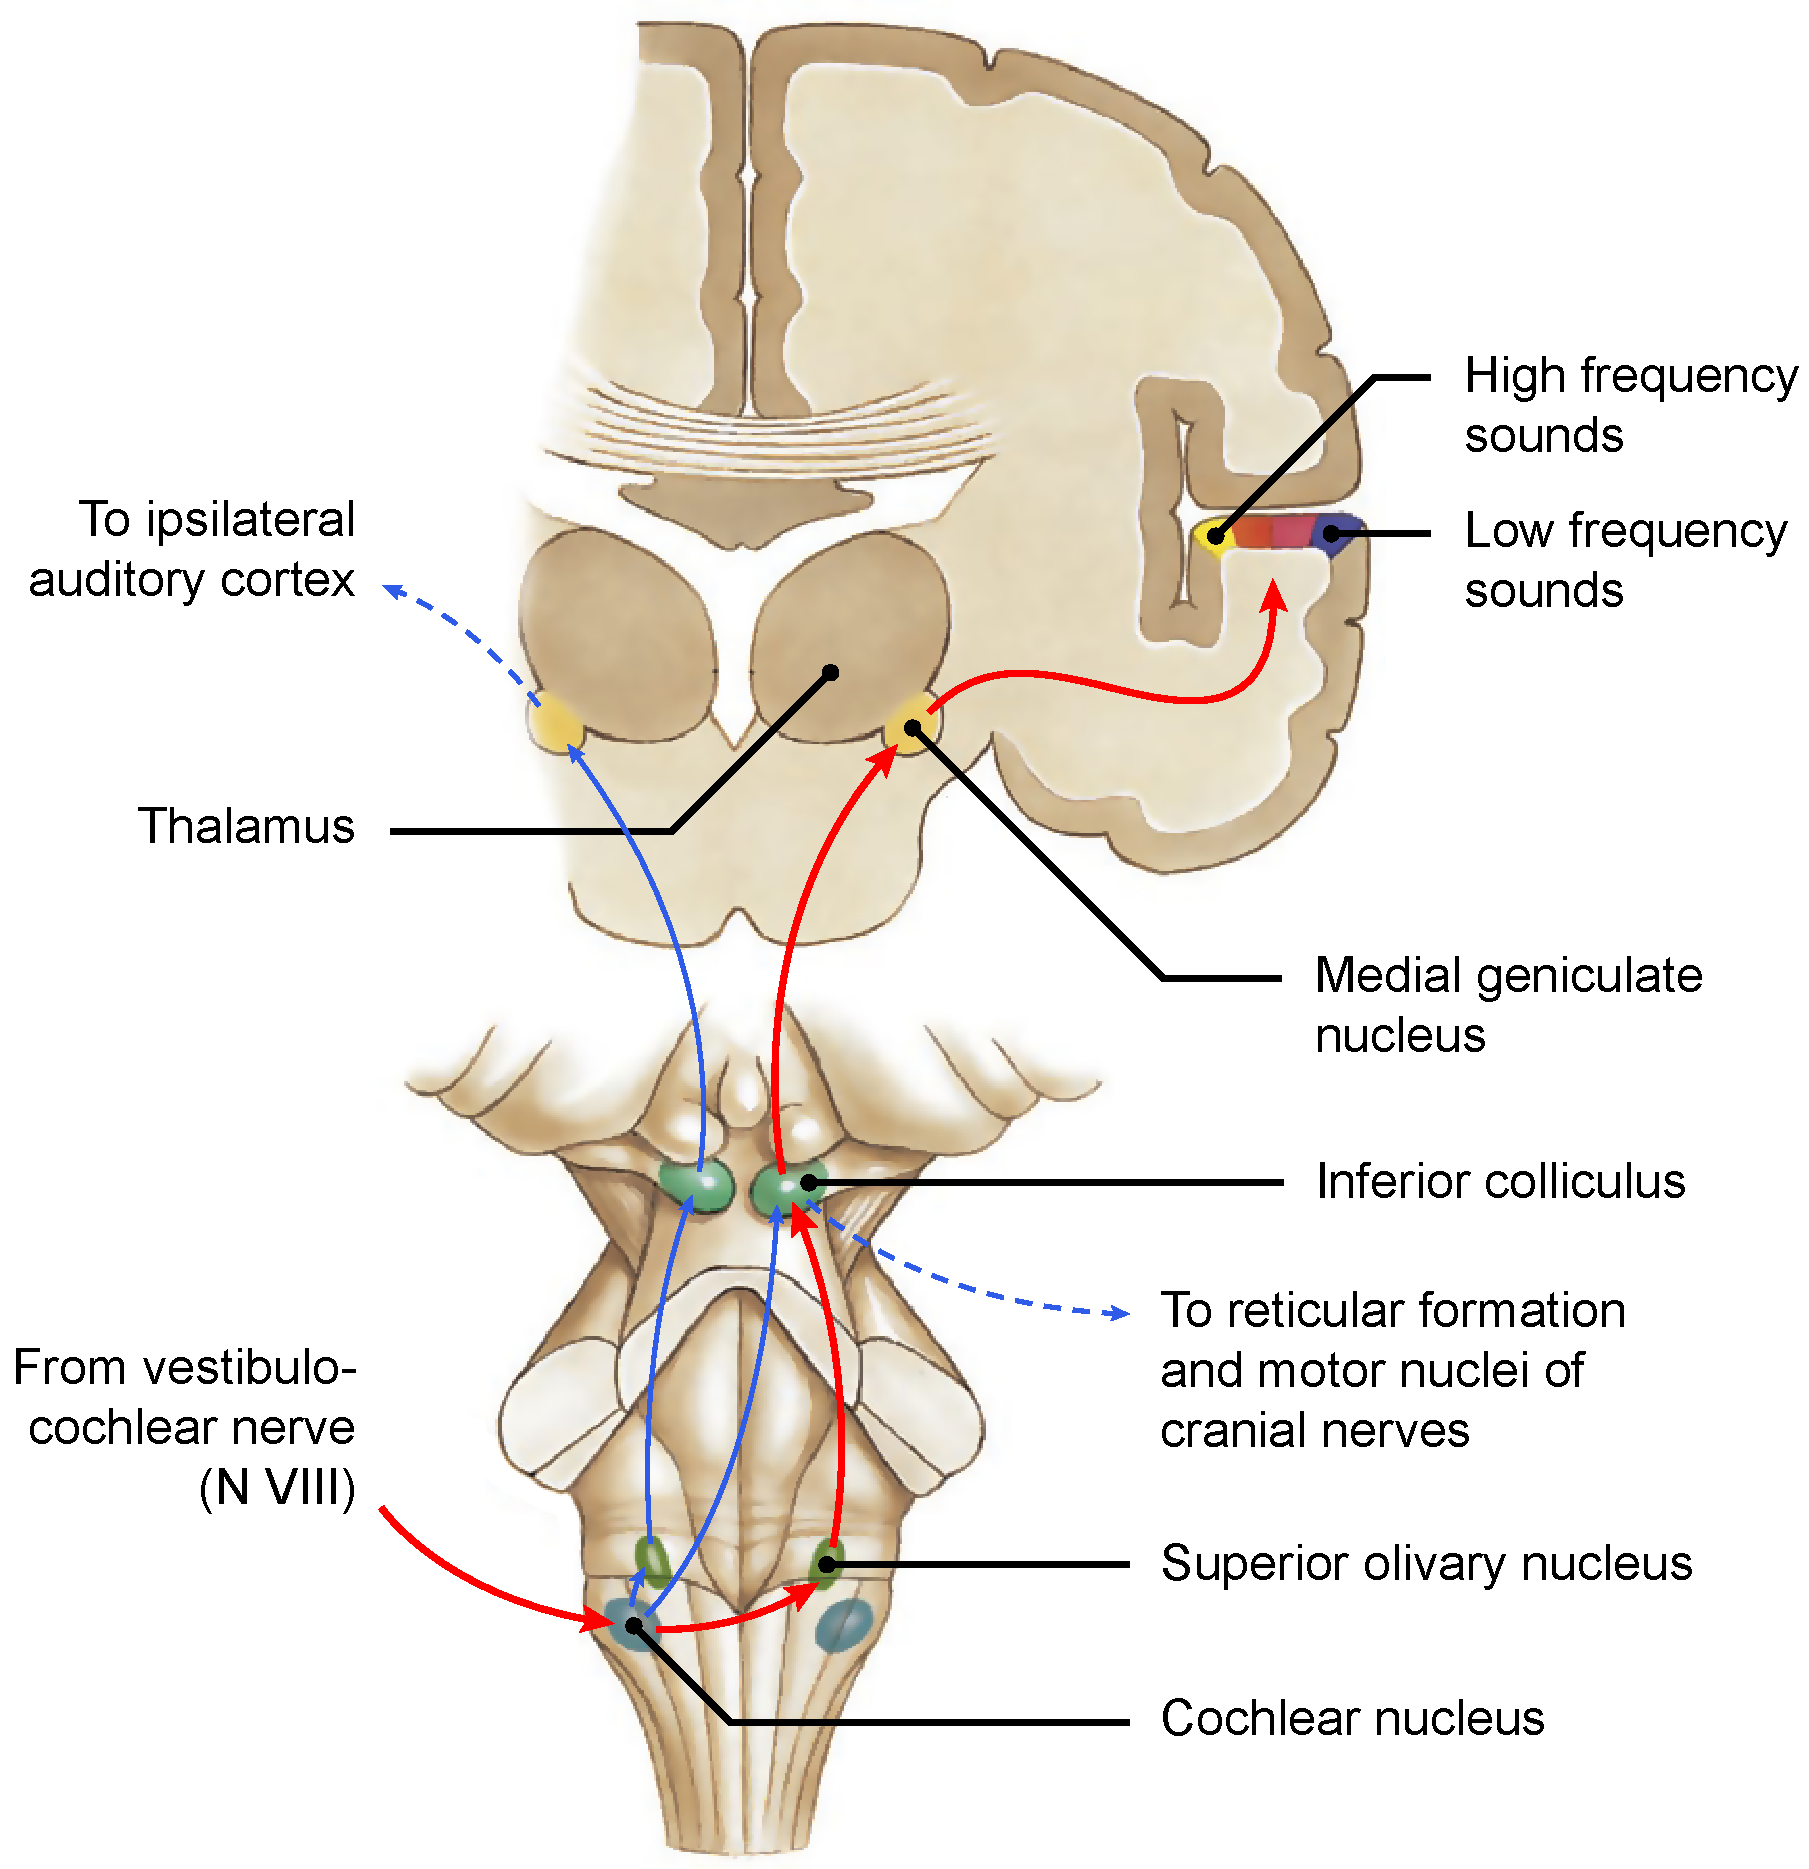
\includegraphics[width=12cm]{Background/cortex_labelled.pdf}
	\caption[Neural pathways to the auditory cortex]{Neural pathways to the
	auditory cortex. The primary pathway is shown by the red arrows, while
	secondary connections are marked by the blue arrows. The low and high
	frequency regions of the auditory cortex are arranged sequentially, analogous
	to the tonotopic organisation of the cochlea (cf. Figure~\ref{fig:tonotopy}).
	(Image adapted from Martini~\etal~\cite{martini2006}. Copyright
	\textcopyright{} 2006, Daryl Fox.)}
	\label{fig:auditory_cortex}
\end{figure}

% ============================================================= Cochlear anatomy

\subsection{Detailed Structure of the Cochlea}
\label{section:cochlea_detail}

The cochlea is a biological electromechanical system with three main classes of
internal structures: fluid spaces and structural support, sensory neuroanatomy,
and vasculature. Each of these is comprised of different tissue types and plays
a unique but interdependent role in the hearing process.

\subsubsection{Directional Terms}

Due to its tapered spiral shape, directions in the cochlea are usually described
relative to the \emph{mid-modiolar axis}, i.e. the axis through the centre of
the cochlea around which the labyrinths spiral (see
Figure~\ref{fig:directions}). There is also a consensus cochlear coordinate
system for quantitative measurements~\cite{verbist2010}. The key terms used in
this thesis are listed below:

\begin{description}
	\item[\textsf{Apical---Basal}] Any axis parallel to the mid-modiolar axis.
	\item[\textsf{Above---Below}] Towards the apex/base of the cochlea. Used when
	describing structures in a localised region.
	\item[\textsf{Radial}] Any axis perpendicular to the mid-modiolar axis.
	\item[\textsf{Medial---Lateral, or Central---Peripheral}] Towards/away from the
	mid-modiolar axis along a radial axis. The former pair is usually used in the
	context of a cross-sectional slice, while the latter pair is used in reference
	to the three-dimensional (3D) structure.
	\item[\textsf{Spiral}] The helical path followed by the labyrinths around the
	mid-modiolar axis.
	\item[\textsf{Turn}] A 360 degree segment of the cochlear spiral.
\end{description}

\begin{figure}
	\centering
	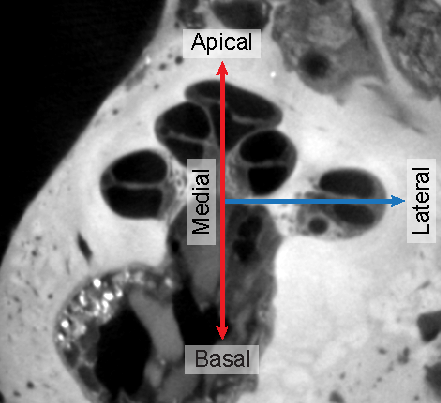
\includegraphics[height=7cm]{Background/directions}
	\caption[Directional terms in the cochlear region]{Directional terms in the
	cochlear region. The mid-modiolar axis is shown in red, and a radial axis in
	blue.}
	\label{fig:directions}
\end{figure}

\subsubsection{Fluid Spaces and Structural Support}

At the highest level, the cochlea is dominated by the bony and membranous
labyrinths. In the vestibular complex, the membranous labyrinth is attached to
the bony labyrinth along one side. In the cochlea, however, the continuation of
the membranous labyrinth, known as the \emph{scala media}, is sandwiched between a
pair of perilymphatic ducts, the \emph{scala vestibuli} and the \emph{scala
tympani} (see Figure~\ref{fig:cochlea}). The former leads up the spiral from the
oval window, and is continuous at the \emph{helicotrema} with the latter, which
heads back down the spiral and ends at a second opening in the cochlear wall
called the \emph{round window}.

\begin{figure}[p]
	\centering
	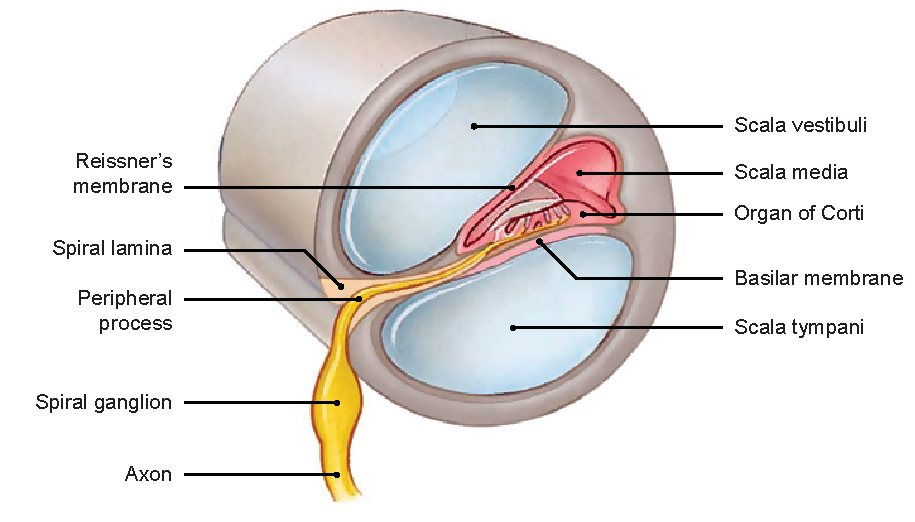
\includegraphics[width=14.6cm]{Background/cochlear_turn}
	\caption[Sectional view through one turn of the cochlea]{Sectional view
	through one turn of the cochlea. (Image adapted from
	Tate~\cite{tate2012}. Copyright \textcopyright{} 2012, McGraw Hill.)}
	\label{fig:cochlea}
\end{figure}

The upper and lower boundaries of the scala media are formed by two thin
membranes---\emph{Reissner's membrane} and the \emph{basilar membrane}---which
separate it from the scala vestibuli and the scala tympani, respectively. Its
lateral border is the \emph{spiral ligament}, which is attached to the bone of
the lateral wall (Figure~\ref{fig:corti}). A capillary bed known as the
\emph{stria vascularis} forms on the upper portion of the spiral ligament at its
junction with the scala media. Along with the spiral ligament and the epithelial
supporting cells, the stria vascularis plays an important role in maintaining
the ionic composition of the endolymphatic space~\cite{flint2010}.

\begin{figure}[p]
	\centering
	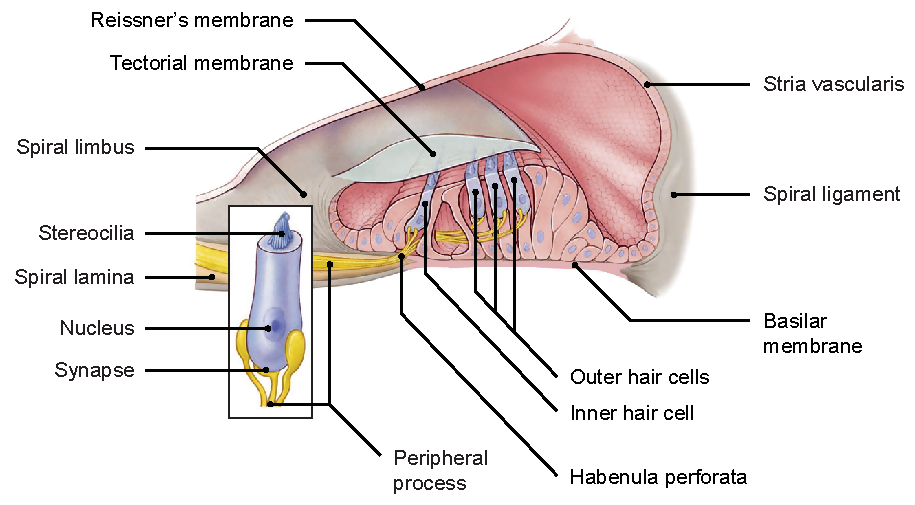
\includegraphics[width=15cm]{Background/corti_hair_cell}
	\caption[The organ of Corti]{The organ of Corti within the scala media.
	Inset shows the basic structure of an isolated hair cell. (Image adapted from
	Tate~\cite{tate2012}. Copyright \textcopyright{} 2012, McGraw Hill.)}
	\label{fig:corti}
\end{figure}

The scala media only spans part of the radial distance from the lateral wall to
the bony core of the cochlea, known as the \emph{modiolus}. The remaining
distance is occupied by the \emph{spiral lamina}, a double-layer bony plate that
extends outwards from the modiolus to meet the basilar membrane. The space
between the plates is occupied by the auditory neurons as they pass through to
the modiolus, as detailed in the next section.

All of these structures together wrap around the modiolus along the helical path
of the scalae. Starting from the round window, the first four quadrants comprise
the basal turn, the next four the middle turn, and the remainder the apical
turn. Erixon \etal~\cite{erixon2009} studied 73 corrosion casts of adult human
inner ears and found that an average human cochlea has 2.6 turns. The
observed range of 2.2--2.9 turns indicates considerable variation between
individuals. The study also revealed variations in other key dimensions; these
measurements are summarised in Table~\ref{table:cochlea_dimensions}.

\begin{table}
	\centering
	\sffamily
	\small
	
	\caption[Key dimensions of the adult human cochlea]{Key dimensions of the adult
	human cochlea. (Data from Erixon~\etal~\cite{erixon2009}.)}
	\label{table:cochlea_dimensions}
	
	\begin{subtable}[t]{0.47\textwidth}
        \caption{Outer wall length.}
        \label{table:dimensions_outer_wall}

        \begin{tabularx}{\textwidth}{X c c}
			\toprule
			\textbf{Location} 	& \textbf{~~Mean $ \boldsymbol\pm $ SD~~}	& \textbf{~~~Range~~~~}\\
								& \textbf{(mm)}								& \textbf{(mm)} \\
			\midrule
			
			First turn		& 22.6 $ \pm $ 0.83 		& 20.3--24.3\\
			Second turn		& 12.4 $ \pm $ 0.63 		& 10.7--13.3\\
			Third turn		& 6.1 $ \pm $ 1.40			& 1.5--8.2\\[1.5mm]
			\emph{Total}	& 42.0 $ \pm $ 1.96			& 38.6--45.6\\
			
			\bottomrule
		\end{tabularx}
		
    \end{subtable}
    
    \vspace{1em}
	\begin{subtable}[t]{0.47\textwidth}
        \caption{Height.}
        \label{table:dimensions_height}

        \begin{tabularx}{\textwidth}{X c c}
			\toprule
			\textbf{Location} 	& \textbf{~~Mean $ \boldsymbol\pm $ SD~~}	& \textbf{~~~Range~~~~}\\
								& \textbf{(mm)}								& \textbf{(mm)} \\
			\midrule
			
			First turn		& 2.1 $ \pm $ 0.20			& 1.6--2.6\\
			Second turn		& 1.2 $ \pm $ 0.17 			& 0.8--1.6\\
			Third turn		& 0.6 $ \pm $ 0.18 			& 0.3--1.1\\[1.5mm]
			\emph{Total}	& 3.9 $ \pm $ 0.37 			& 3.3--4.8\\
			
			\bottomrule
		\end{tabularx}
		
    \end{subtable}
    
    \vspace{1em}
	\begin{subtable}[t]{0.47\textwidth}
        \caption{Width.}
        \label{table:dimensions_width}

        \begin{tabularx}{\textwidth}{X c c}
			\toprule
			\textbf{Location} 	& \textbf{~~Mean $ \boldsymbol\pm $ SD~~}	& \textbf{~~~Range~~~~}\\
								& \textbf{(mm)}								& \textbf{(mm)} \\
			\midrule
			
			First turn		& 6.8 $ \pm $ 0.46			& 5.6--8.2\\
			Second turn		& 3.8 $ \pm $ 0.25			& 3.3--4.3\\
			Third turn		& 2.1 $ \pm $ 0.52			& 0.6--3.6\\
			\bottomrule
		\end{tabularx}
		
    \end{subtable}
    
\end{table}

\subsubsection{Neural Structures}

The cornerstone of the hearing mechanism is the hair cell (see inset,
Figure~\ref{fig:corti}) in that these cells are responsible for the actual
transduction of physical vibrations that make up sound waves to neural impulses.
They are housed within the \emph{organ of Corti}, which is named after its
discoverer, Alfonso Corti~\cite{jahn2001}. Figure~\ref{fig:corti} depicts the
positions of the hair cells within the organ of Corti. They are embedded in
epithelial supporting cells that lie on the basilar membrane and are organised
into one inner row and three outer rows. \emph{Stereocilia} protruding from the
exposed surface of each hair cell are attached the overlying \emph{tectorial
membrane}, which itself is anchored to the medial wall of the scala media via
the \emph{spiral limbus}.

There are about 15,000 hair cells in the human inner ear, split into 3,000 inner
hair cells and 12,000 outer hair cells~\cite{nadol1993,flint2010}. These are
monitored by the \emph{peripheral processes} of the bipolar auditory neurons.
The processes leave the organ of Corti and enter the space between the double
wall of the spiral lamina via tiny openings called the \emph{habenula
perforata}. From here, they travel centrally to Rosenthal's canal, wherein the
cell bodies of the neurons lie and together form the spiral ganglion. Their
myelinated axons then run towards the base of the cochlea, combining to form the
cochlear branch of N VIII. Most of the auditory neurons are afferent, but there
are also some efferent fibres that lead back towards the hair cells to form a
feedback loop.

\subsubsection{Vascular Structures}
\label{sect:cochlear_vessels}

Traditional descriptions of the cochlea have generally excluded its vasculature.
The most comprehensive investigation of the cochlear vessels is a survey by
Axelsson~\cite{axelsson1968}, which encompassed work by pioneers such as
Ibsen~\cite{ibsen1881} and Schwalbe~\cite{schwalbe1887} in the 19th century on
animal specimens, as well as later studies of the human system by
Eichler~\cite{eichler1892}, Siebenmann~\cite{siebenmann1894},
Nabeya~\cite{nabeya1923}, and Scuderi and Del Bo~\cite{scuderi1952}. The
information provided by these authors was at times incomplete and
conflicting~\cite{axelsson1968}, which is not unexpected given the limitations
in existing imaging technology and the complexity of the cochlear vasculature
(cf. Siebenmann's illustration in Figure~\ref{fig:siebenmann}). Axelsson went on
to unify the previous work, so the information in the remainder of this section
is drawn predominantly from his account.

\begin{figure}
	\centering
	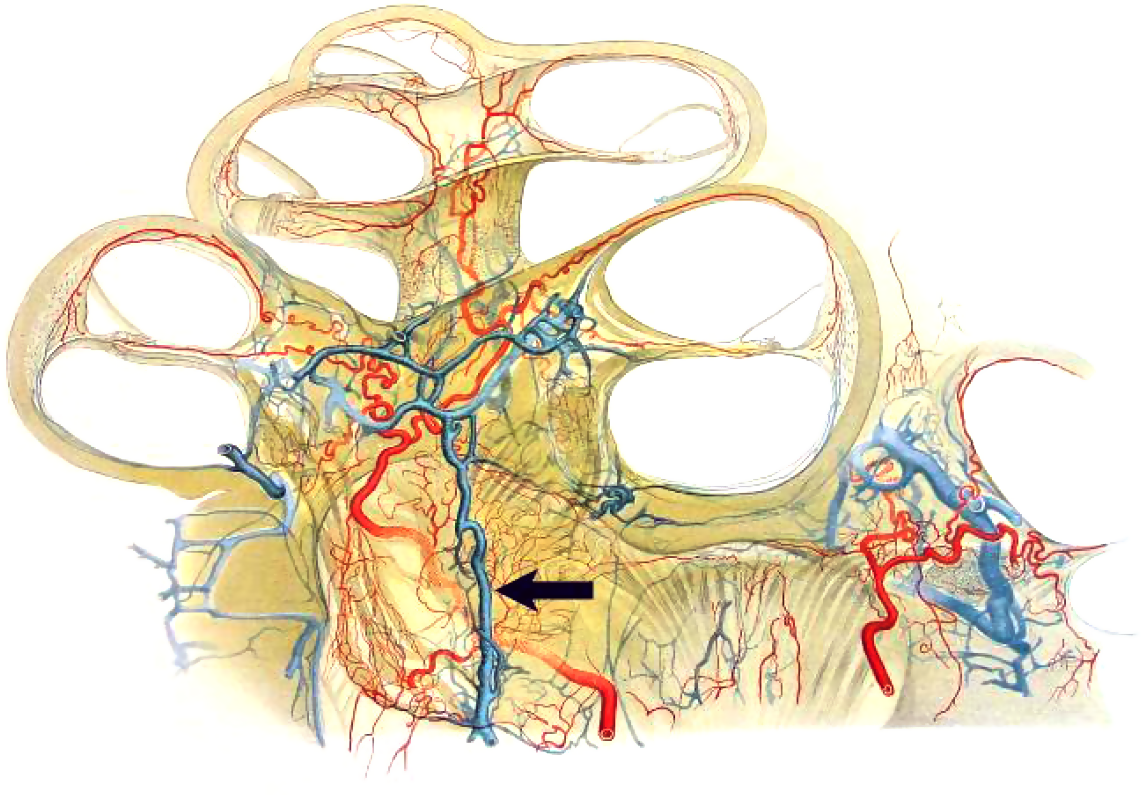
\includegraphics[height=7.5cm]{Background/siebenmann}
	\caption[Sketch of the cochlear vasculature]{Sketch of the cochlear vasculature
	by Siebenmann, demonstrating the intricate structure of the blood vessel
	network. The black arrow indicates the ``central auditory vein'', which likely
	refers to what is now termed the ``common modiolar vein'' (cf.
	Figure~\ref{fig:venous_drainage}). (Source: Siebenmann~\cite{siebenmann1894}.)}
	\label{fig:siebenmann}
\end{figure}

The origin of the cochlear blood supply can be traced back to the
\emph{brachiocephalic trunk}. From here, the arterial path typically follows the
vertebral, basilar, anterior inferior cerebellar, and labyrinthine arteries in
order as shown in Figure~\ref{fig:arterial_supply}, though slight variations may
exist amongst individuals. In either case, the \emph{labyrinthine artery} is
usually the sole supplier of blood to the cochlea. It follows N VIII through the
\emph{internal acoustic meatus}, and branches to form the \emph{anterior
vestibular artery} (AVA) and the \emph{common cochlear artery}. The latter then
divides into the \emph{vestibulo-cochlear artery} (VCA) and the \emph{spiral
modiolar artery} (SMA).

\begin{figure}
	\centering
	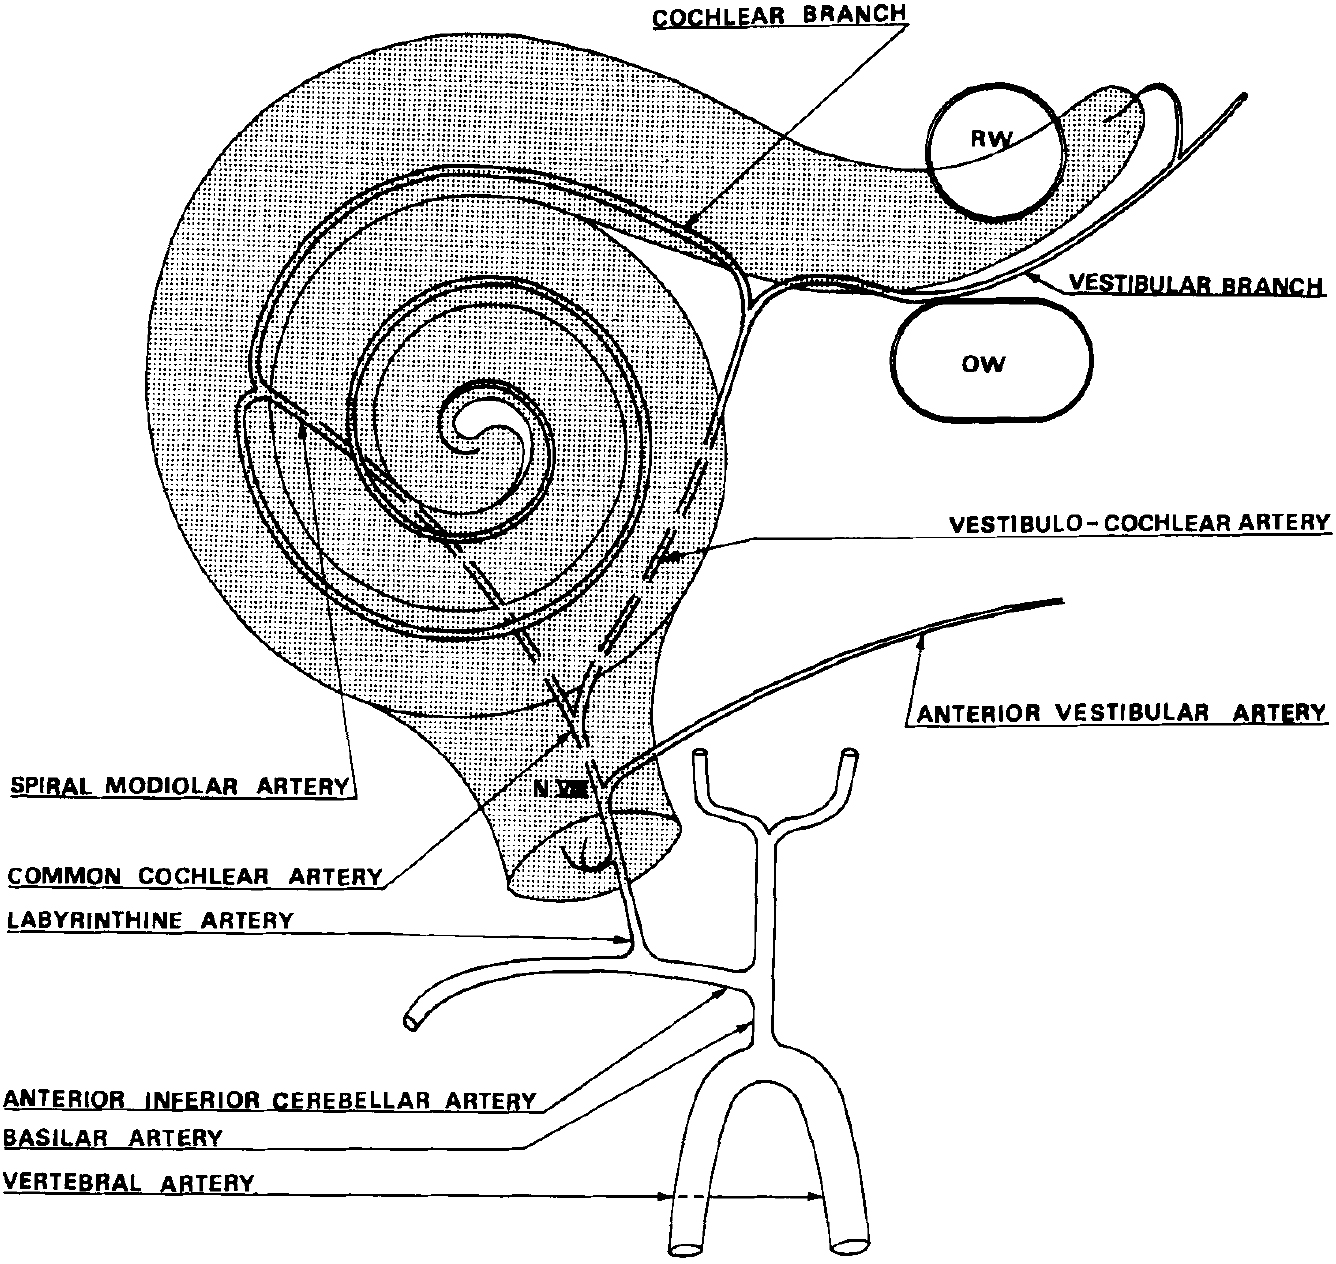
\includegraphics[height=11.5cm]{Background/arterial_supply}
	\caption[Schematic of the cochlear arterial supply in man]{Schematic of the
	cochlear arterial supply in man. OW=oval window; RW=round window; N
	VIII=vestibulocochlear nerve. (Source: Axelsson~\cite{axelsson1968}. Copyright
	\textcopyright{} 1968, Taylor \& Francis.)}
	\label{fig:arterial_supply}
\end{figure}

Each of these three terminal branches leads to a different region of the inner
ear. The AVA supplies the posterior vestibule and the lateral and anterior
semicircular canals~\cite{leblanc1999}. The VCA enters the modiolus near the
bottom of the basal turn and splits into the \emph{vestibular branch} and the
\emph{cochlear branch}, which run basally and apically along the spiral
respectively. The former supplies the basal-most end of the cochlea, the
posterior semicircular canal and the vestibule, while the latter supplies about
a third of the basal turn before anastomosing with the SMA. This third terminal
branch supplies the remaining majority of the cochlea and is therefore the most
important.

Upon entering the second quadrant of the basal turn, the SMA runs apically,
spiralling around the nerve trunk until it reaches the helicotrema (see
Figure~\ref{fig:modiolar_vessels}). Internal and external \emph{radiating
arterioles} regularly branch off normal to the helical path, feeding capillary
beds in the modiolus, the spiral lamina and the external wall. The capillaries
rejoin, forming \emph{collecting venules} that drain into the cochlear veins.
These radial vessels are shown in Figure~\ref{fig:rad_vessels}.

\begin{figure}
	\centering
	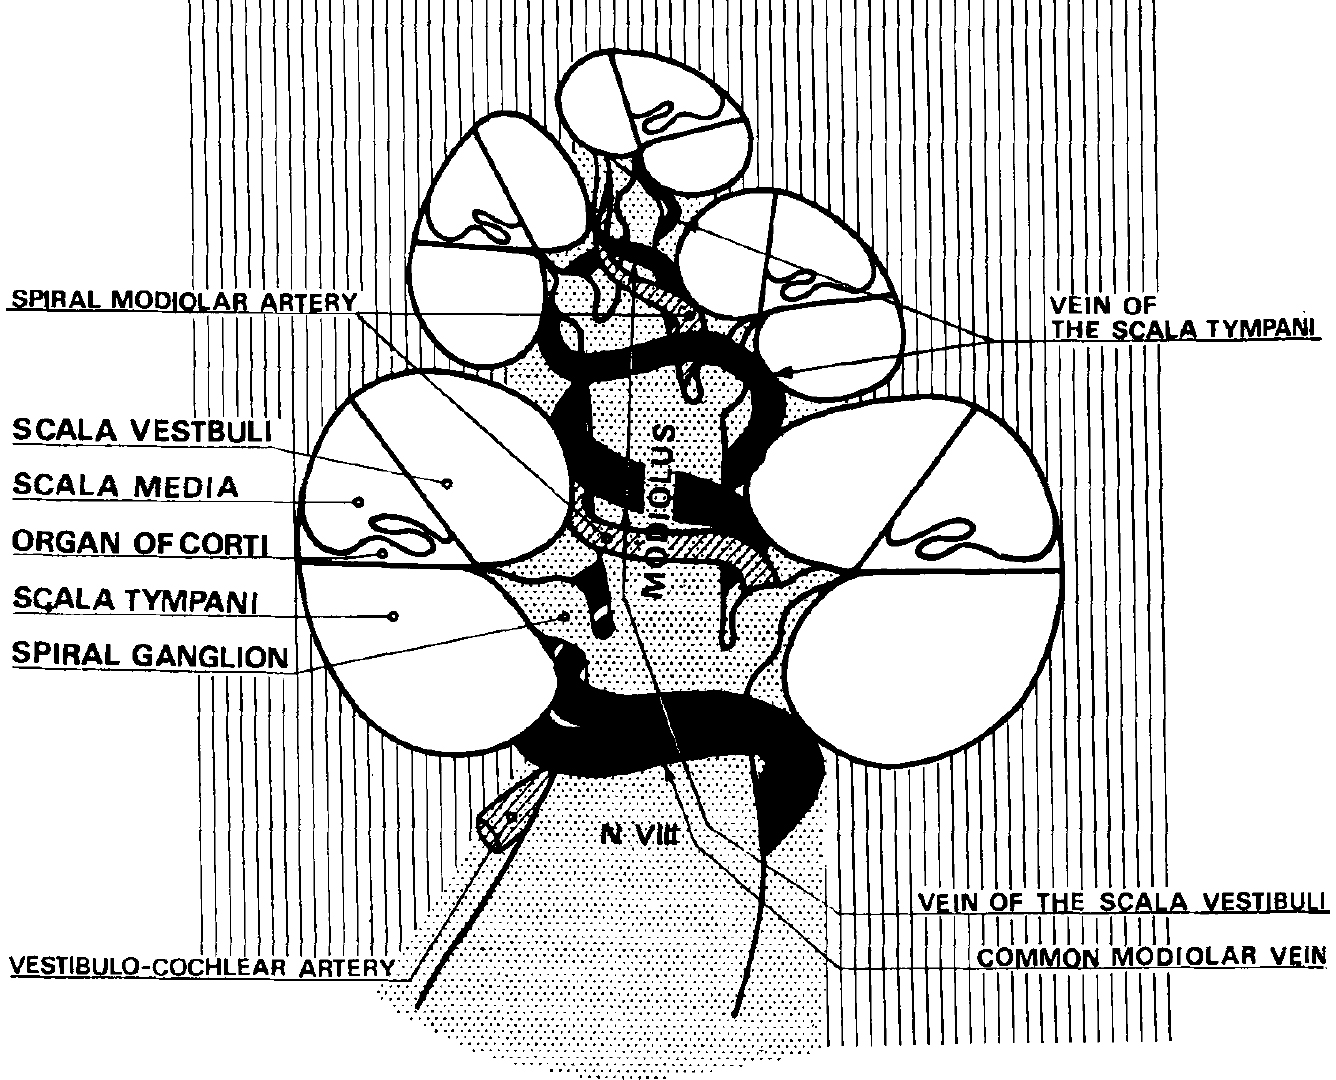
\includegraphics[height=9.2cm]{Background/modiolar_vessels}
	\caption[Cross-sectional schematic of the modiolar vessels in
	man]{Cross-sectional schematic of the modiolar vessels in man. (Source:
	Axelsson~\cite{axelsson1968}. Copyright \textcopyright{} 1968, Taylor \&
	Francis.)}
	\label{fig:modiolar_vessels}
\end{figure}

\begin{figure}
	\centering
	
    \begin{subfigure}[t]{0.53\textwidth}
        \centering
        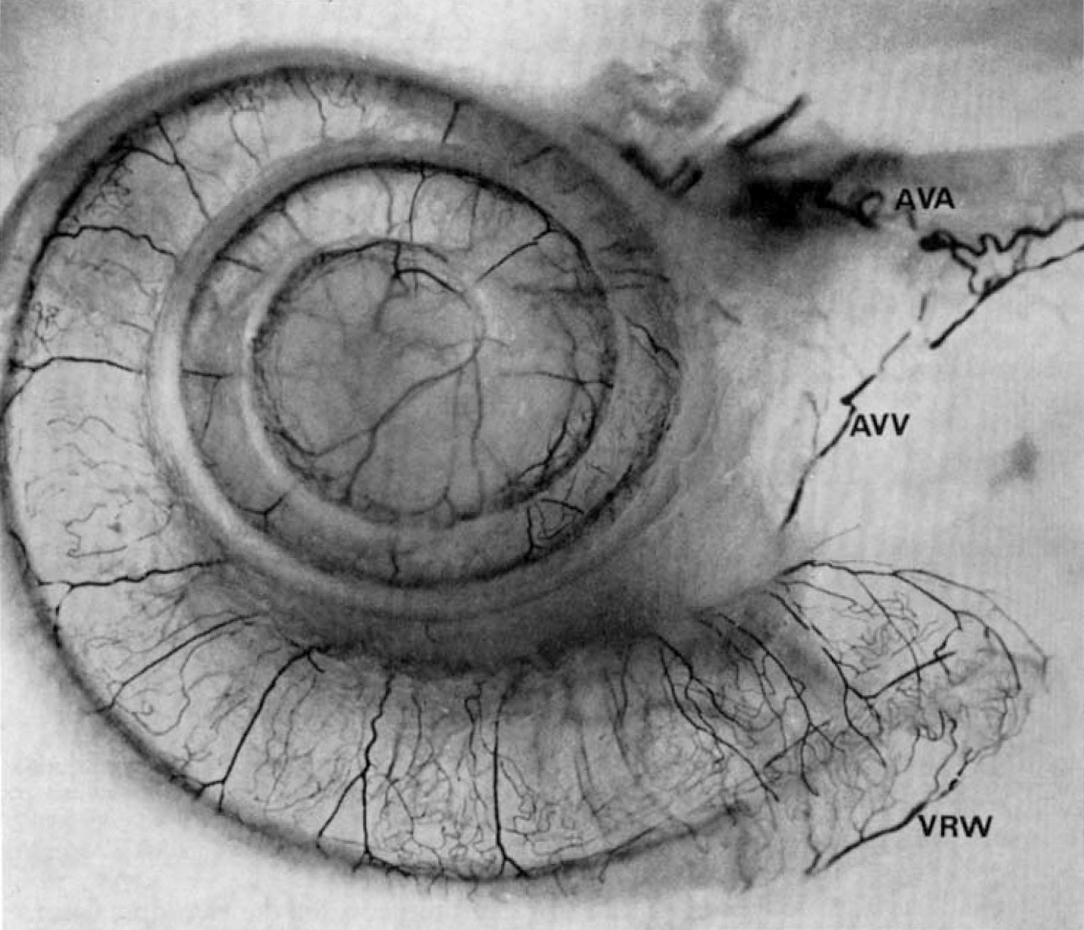
\includegraphics[height=6.5cm]{Background/radart}
        \caption{ }
        \label{fig:rad_art_top}
    \end{subfigure}
	~
	\begin{subfigure}[t]{0.45\textwidth}
        \centering
        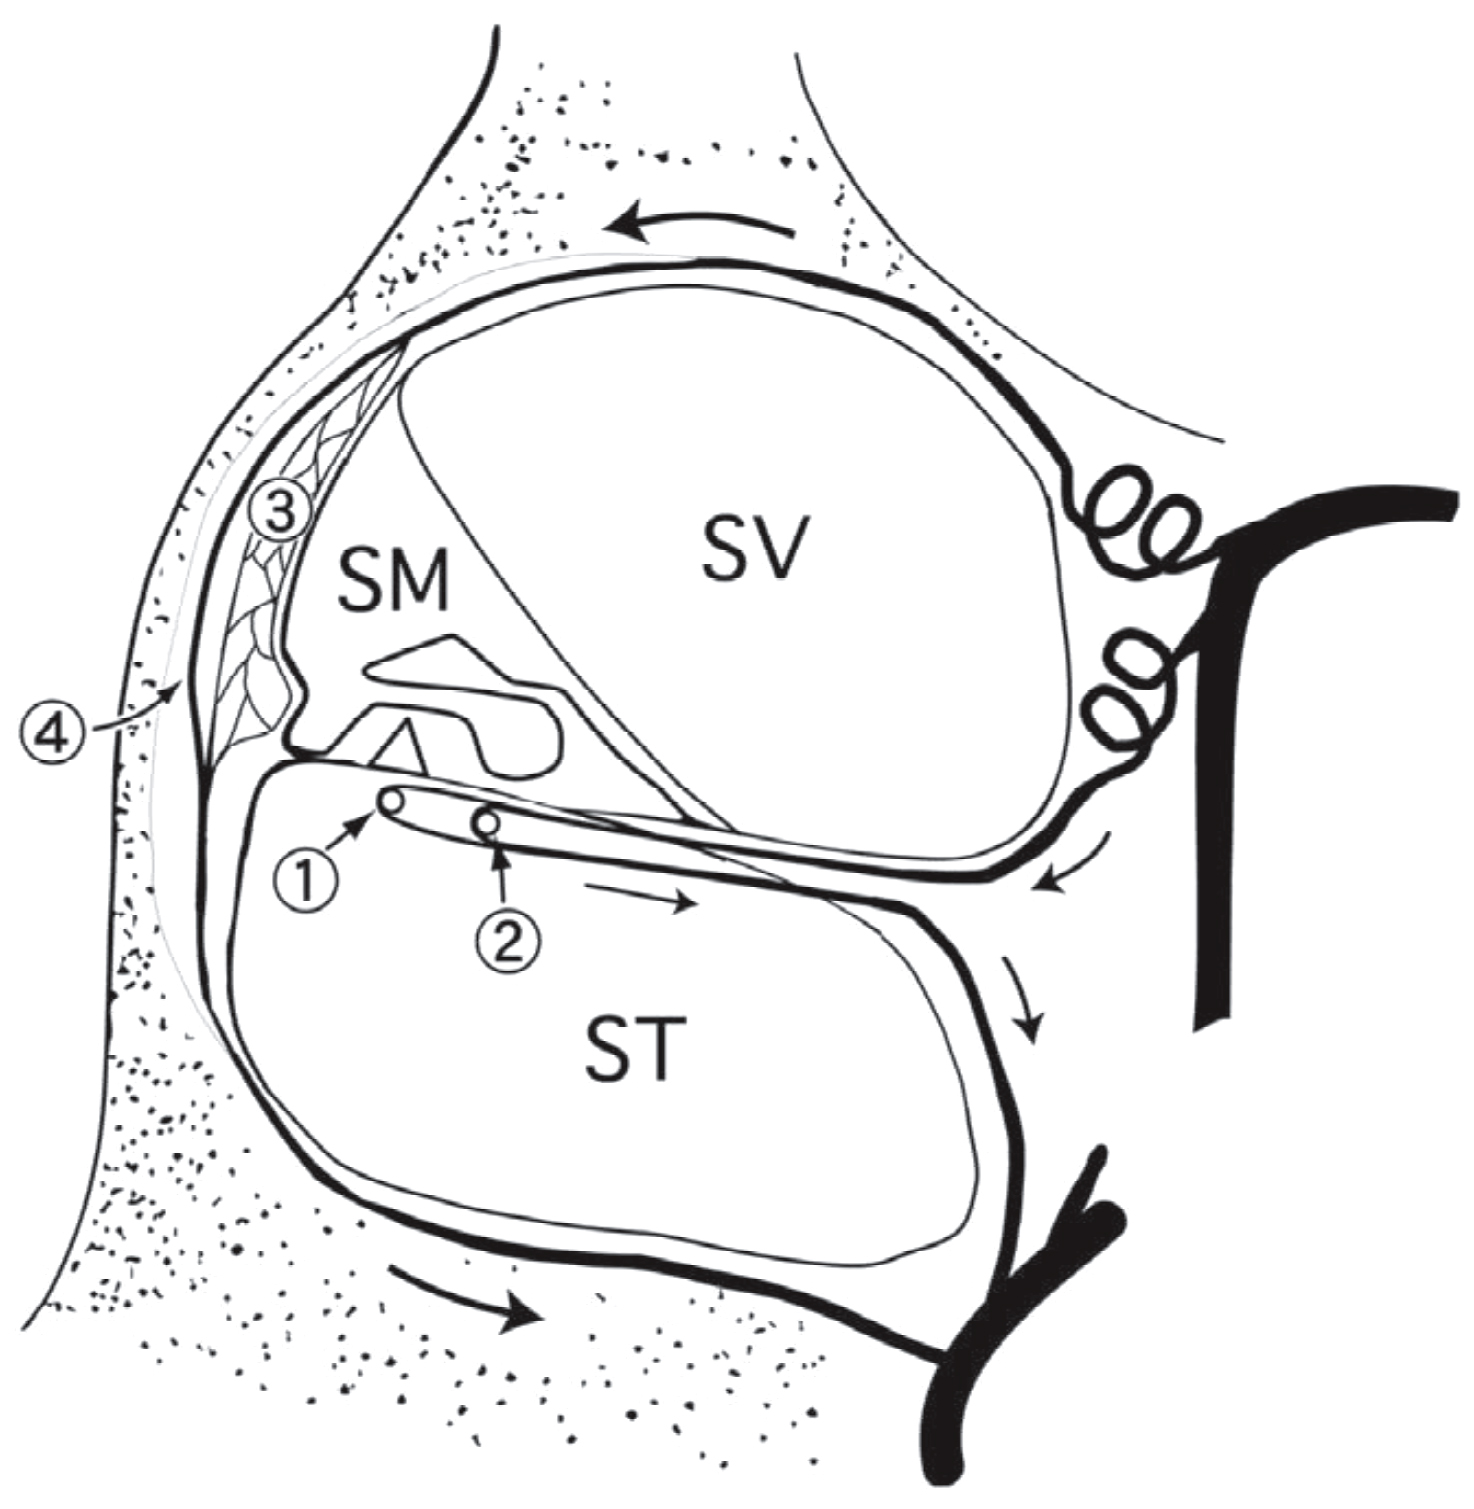
\includegraphics[height=6.5cm]{Methodology/vesselsinturn}
        \caption{ }
        \label{fig:rad_art_section}
    \end{subfigure}
    
	\caption[Radiating arterioles and collecting venules]{(a) Radiating arterioles
	(darker) and collecting venules (lighter) in the human cochlea. AVA=anterior
	vestibular artery; AVV=anterior vestibular vein; VRW=vein of the round window.
	(Source: Axelsson~\cite{axelsson1968}. Copyright \textcopyright{} 1968, Taylor
	\& Francis.) (b) Schematic view through one turn of the cochlea. (Source:
	Nakashima~\etal~\cite{nakashima2003}. Copyright \textcopyright{} 2003, Elsevier
	B.V.)}
	\label{fig:rad_vessels}
\end{figure}

Human cochleae exhibit a double venous system, one for the scala vestibuli and
one for the scala tympani. The former is drained along with the spiral lamina by
a discontinuous series of venous segments together known as the \emph{vein of
the scala vestibuli} (VSV), which is located centrally in the modiolar wall (see
Figures~\ref{fig:modiolar_vessels} and \ref{fig:venous_drainage}). Likewise, the
latter is drained with the spiral ganglion and the external wall of the scala
media by the similarly-structured \emph{vein of the scala tympani} (VST). The
VSV and VST merge near the first quadrant of the basal turn to form the common
modiolar vein (CMV). More basally, the \emph{vein of the round window} (VRW)
drains the associated collecting venules. Both the VRW and the CMV join with the
vestibulo-cochlear vein (VCV) to become the vein of the cochlear aqueduct
(VCAQ), which leaves the cochlear region.

\begin{figure}
	\centering
	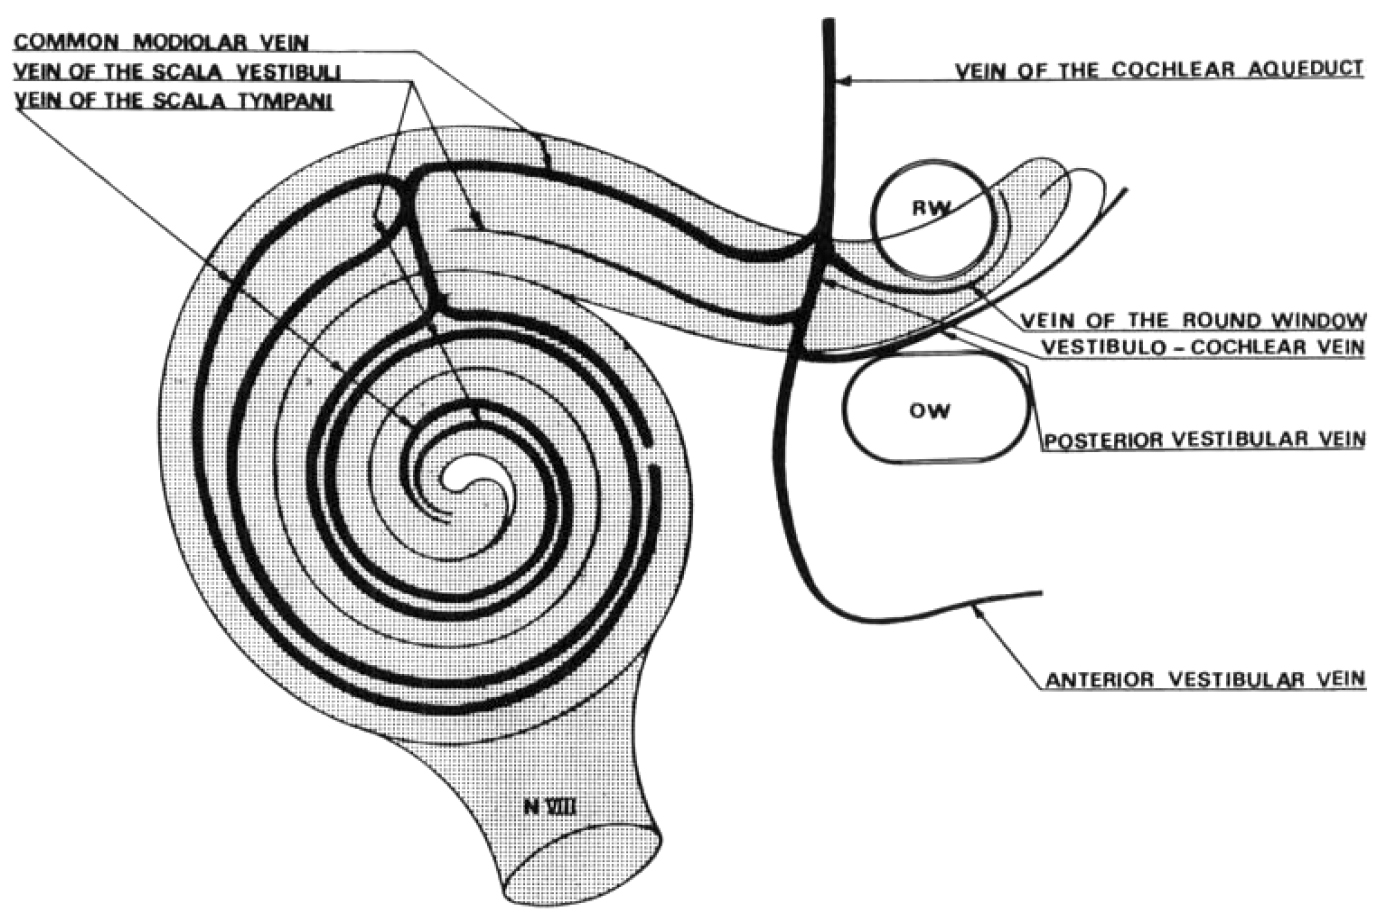
\includegraphics[height=9.2cm]{Background/modiovein}
	\caption[Schematic of the cochlear venous drainage in man]{Schematic of the
	cochlear venous drainage in man. OW=oval window; RW=round window; N
	VIII=vestibulocochlear nerve. (Source: Axelsson~\cite{axelsson1968}. Copyright
	\textcopyright{} 1968, Taylor \& Francis.)}
	\label{fig:venous_drainage}
\end{figure}

Reissner's membrane and some parts of the organ of Corti are avascular.

\subsection{Comparison of Human and Guinea Pig Cochleae}
\label{sect:comparison_of_species}

Although the ultimate goal of cochlear implant (CI) research is to restore the
perception of hearing in humans, the anatomical surroundings of the human
cochlea make \invivo{} testing challenging. The otic capsule surrounding the
cochlea is both thick and extremely dense, and its location deep within the
petrous part of the temporal bone impedes surgical access. Experimental
implantation and probing is unwarranted given the high ratio of risk to benefit.
Cadaveric studies are one alternative, but changes in both the shape and
properties of the tissues post-mortem impede the extrapolation of insights to
living subjects~\cite{ifukube1987,kral1998}.

% The taking of measurements requires probes to be placed within the region of
% interest, but the temporal bone and otic capsule surrounding the cochlea impede
% surgical access. It is possible to penetrate these bones with the correct
% surgical tools, but even then, the phyical invasion of the probes into the
% tissue space would compromise the integrity of the cochlear structures and
% change the measured potentials relative to a true \invivo{} implant. There would
% also be challenges in controlling the positioning of the probe to accurately
% obtain the large number of sample points required to build a detailed
% electro-anatomical map. Furthermore, there are the ethical concerns of such
% experiments on the health and wellbeing of the subjects, whether human or some
% other animal species. Measurements in cadavers may alleviate some of these
% concerns, but physiological changes post-mortem introduce a host of other
% inaccuracies.

Since the mammalian cochlea is similar in both structure and function across
species, many CI studies have been performed on animals---typically cats and
guinea pigs, but also mice, gerbils, rats, chinchillas, and
monkeys~\cite{axelsson1968,greenwood1990,kral1998,zeng2004}. The cochlea of the
guinea pig is commonly used because it is relatively large~\cite{zeng2004} and,
unlike the human cochlea, it is easily exposed in the tympanic
bulla~\cite{cooper1975} (see Figure~\ref{fig:guinea_pig_bulla}), allowing
experimental measurements to be taken relatively easily.
Miyamoto~\cite{miyamoto1986} noted that guinea pig cochleae serve as ``an
appropriate experimental animal model for\ldots[electrophysiological studies] of
cochlear function''.

\begin{figure}[p]
	\centering
	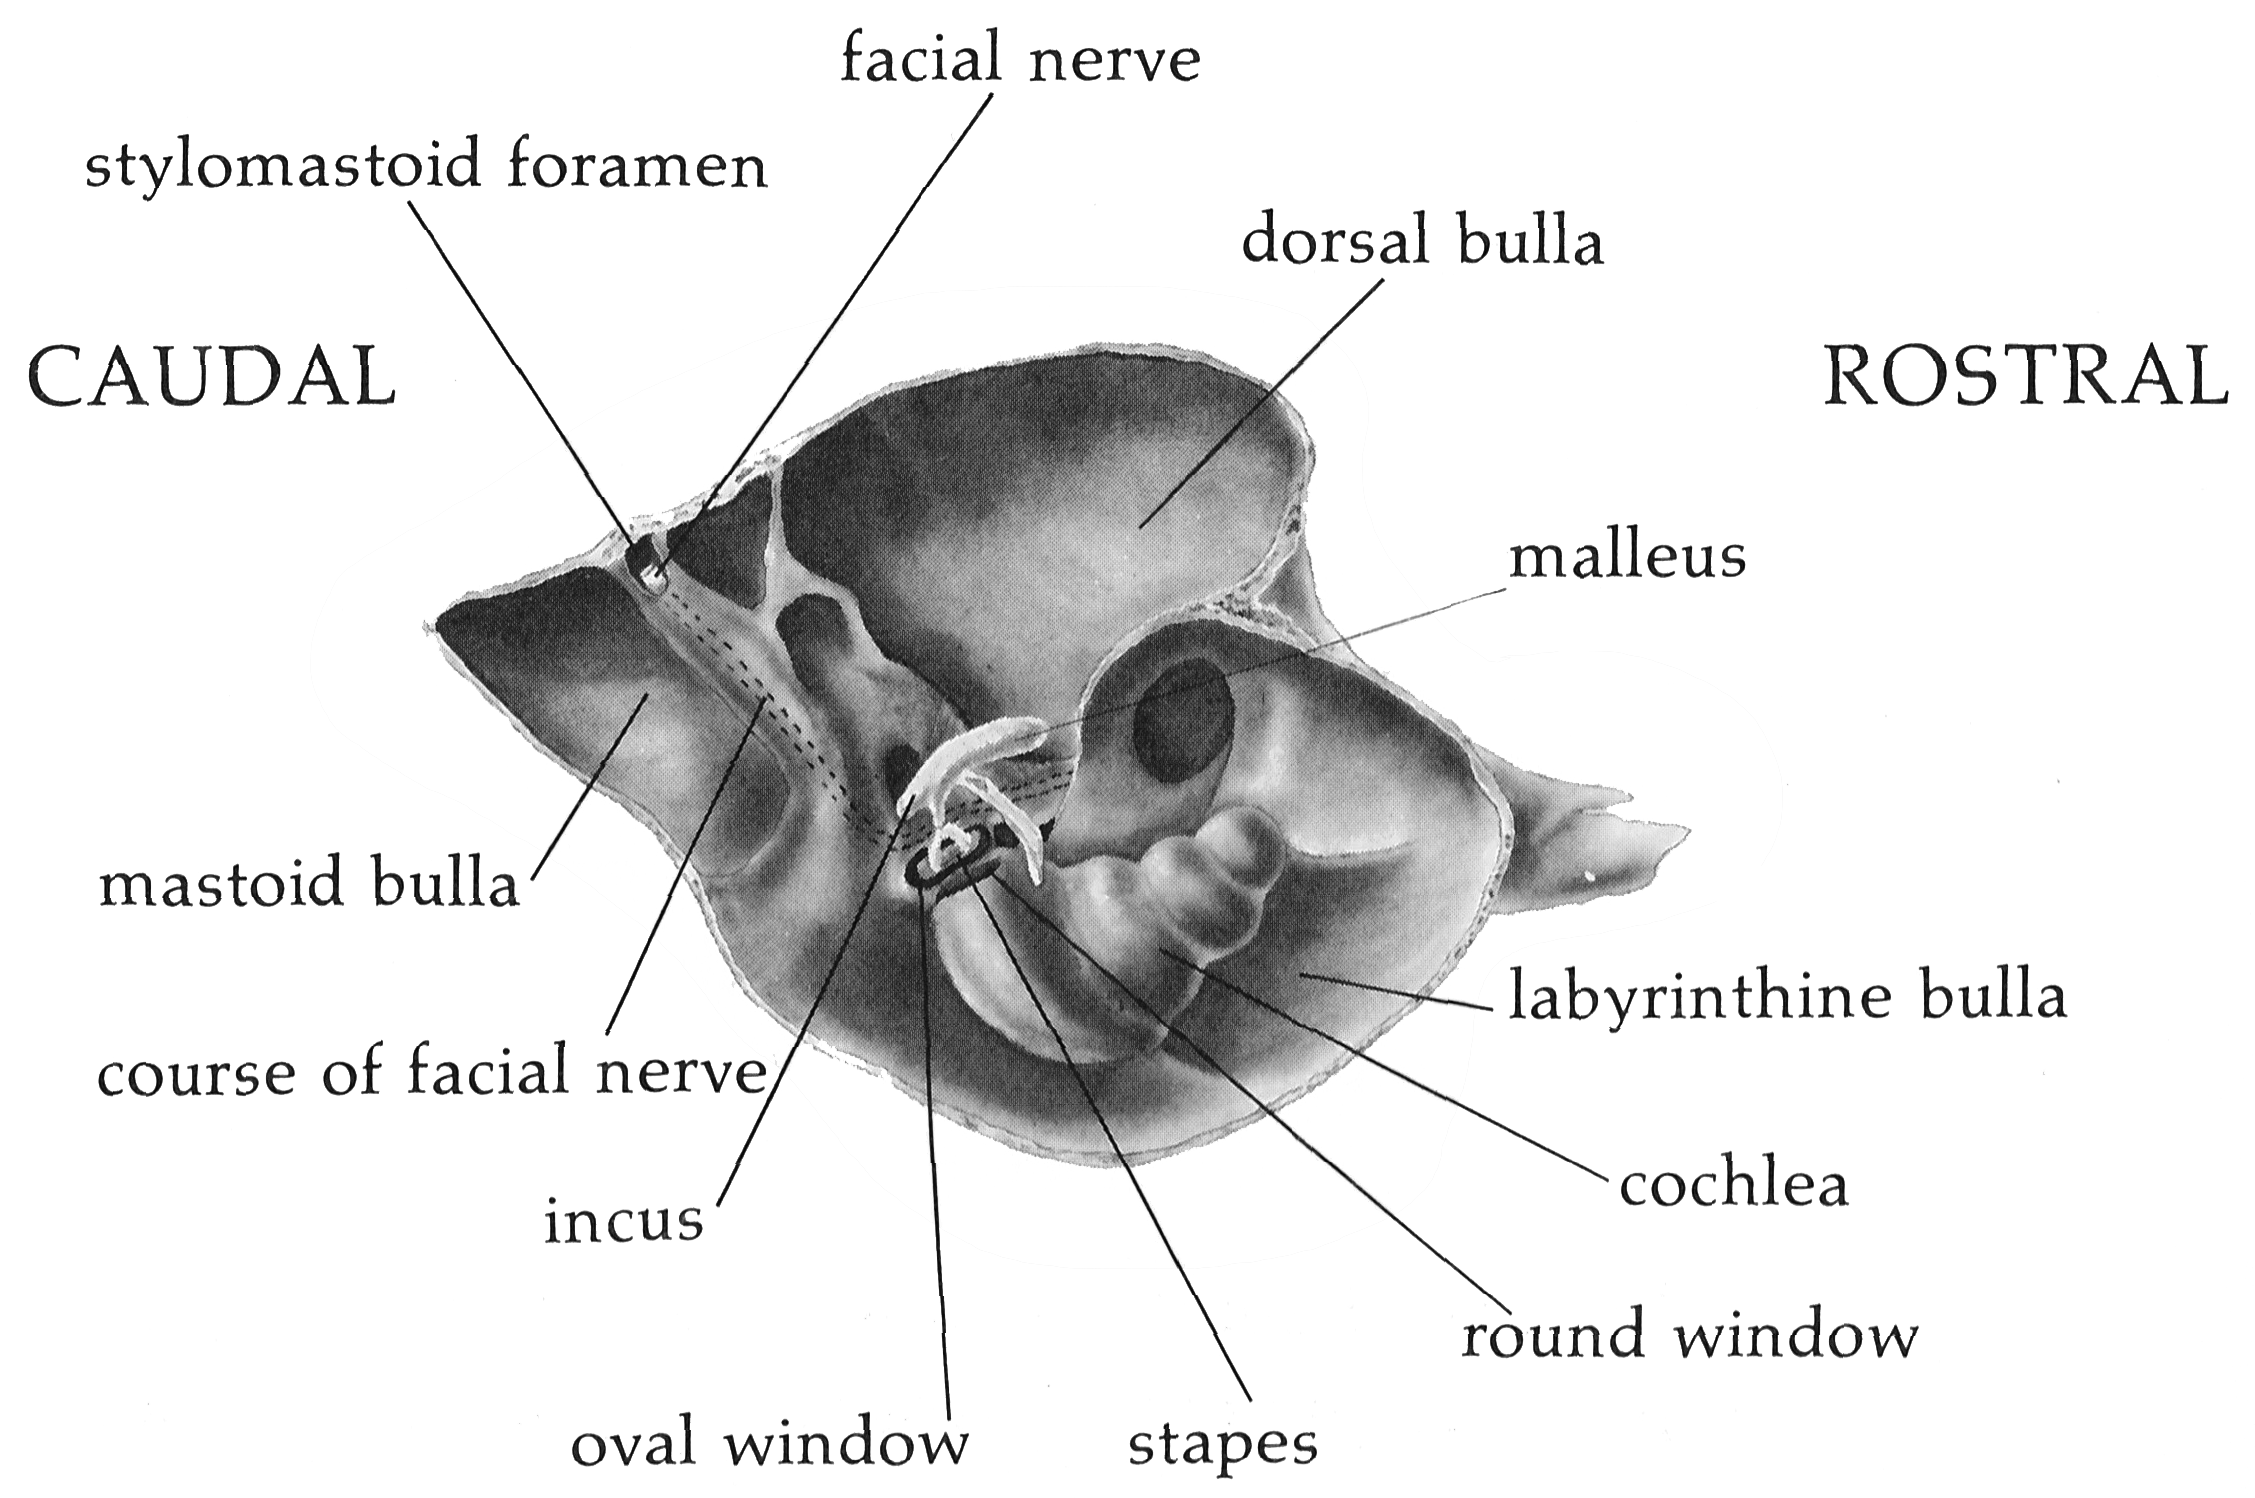
\includegraphics[height=7cm]{Validation/tympanic_bulla}
	\caption[Internal aspect of the tympanic bulla]{Internal aspect of the
	tympanic bulla in the guinea pig. Note how the lateroapical portion of the
	cochlea protrudes into the air space of the tympanic bulla. (Source: Cooper and
	Schiller~\cite{cooper1975}. Copyright \textcopyright{} 1975, Harvard
	University Press.)}
	\label{fig:guinea_pig_bulla}
\end{figure}

Like other mammals, the cochleae of both humans and guinea pigs are comprised
of the cross-sectional structures shown in Figures~\ref{fig:cochlea} and
\ref{fig:corti} spiralling around a nerve-filled modiolus. There are several
notable differences relative to the human cochlea; the main ones are listed in
Table~\ref{table:cochleae_comparison}.

% \item has a relatively large endolymphatic space (by percentage volume) in both
% the cochlea proper and the semicircular canals~\cite{thorne1999};

\begin{table}[p]
	\centering
	\sffamily
	\small
	
	\caption[Comparison of human and guinea pig cochleae]{Comparison of human and
	guinea pig cochleae. Data compiled from various
	sources~\cite{black1980,ota1980,nadol1988comparative,thorne1999,frijns2001,erixon2009}.}
	\label{table:cochleae_comparison}
	
    \begin{tabular}{p{4.5cm} p{4.0cm} p{5.2cm}}
		\toprule
		\textbf{Attribute}	& \textbf{Human}	& \textbf{Guinea pig} \\
		\midrule
		
		Number of turns				& 2.2--2.9				& 3.5--4 \\
		Scalae length				& 26--28~mm				& $ \approx $16~mm \\
		Volume of scala tympani		& 29~$ \upmu $L			& 4.8~$ \upmu $L \\
		Myelination	of spiral ganglion cell bodies		& Rare ($<$5\%) &	Mostly
			myelinated \\
		Geometry of basal end		& Follows spiral trajectory
									& Hooked (turns more parallel with cochlear axis) \\ 
		Location within bone		& Embedded except for the round and oval windows
									& Apex protrudes into tympanic bulla \\
		\bottomrule
	\end{tabular}
		
\end{table}

Since the guinea pig cochlea is not embedded within the petrous part of the
temporal bone, different current pathways are expected~\cite{kral1998}.
These differences mean that although the modelling results may be indicative,
care must be taken when extrapolating results from one species to
another~\cite{frijns2001}.

% ==============================================================================

\section{Hearing Physiology}

\subsection{Normal Hearing}
\label{sect:normal_hearing}

Normal hearing is comprised of two distinct stages: the first (sensation) occurs
when a sound stimulus is detected at the biological receptor; the second
(perception) occurs when a conscious awareness of the sensation is
obtained~\cite{martini2006}. Sensation is therefore clearly a prerequisite for
perception, and any complications in sensing a sound stimulus flow on to impair
the perception of that sound.

The propagation of sound waves through the cochlea is illustrated in
Figure~\ref{fig:travelling_wave}. Sound stimuli consist of pressure waves moving
through a medium, typically air or water. They are funnelled into the external
acoustic meatus by the auricle and detected by the tympanic membrane, which
vibrates in response. These vibrations are mechanically coupled by the auditory
ossicles to the oval window, where the action of the stapes footplate induces
compressional waves in the perilymph. The 20:1 area ratio between the tympanic
membrane and the stapes footplate and the 1.31:1 lever ratio between the moment
arms of the malleus and the incus help to minimise the loss of energy that would
otherwise occur due to the large difference in acoustic impedances between air
and perilymph~\cite{flint2010}.

\begin{figure}
	\centering
	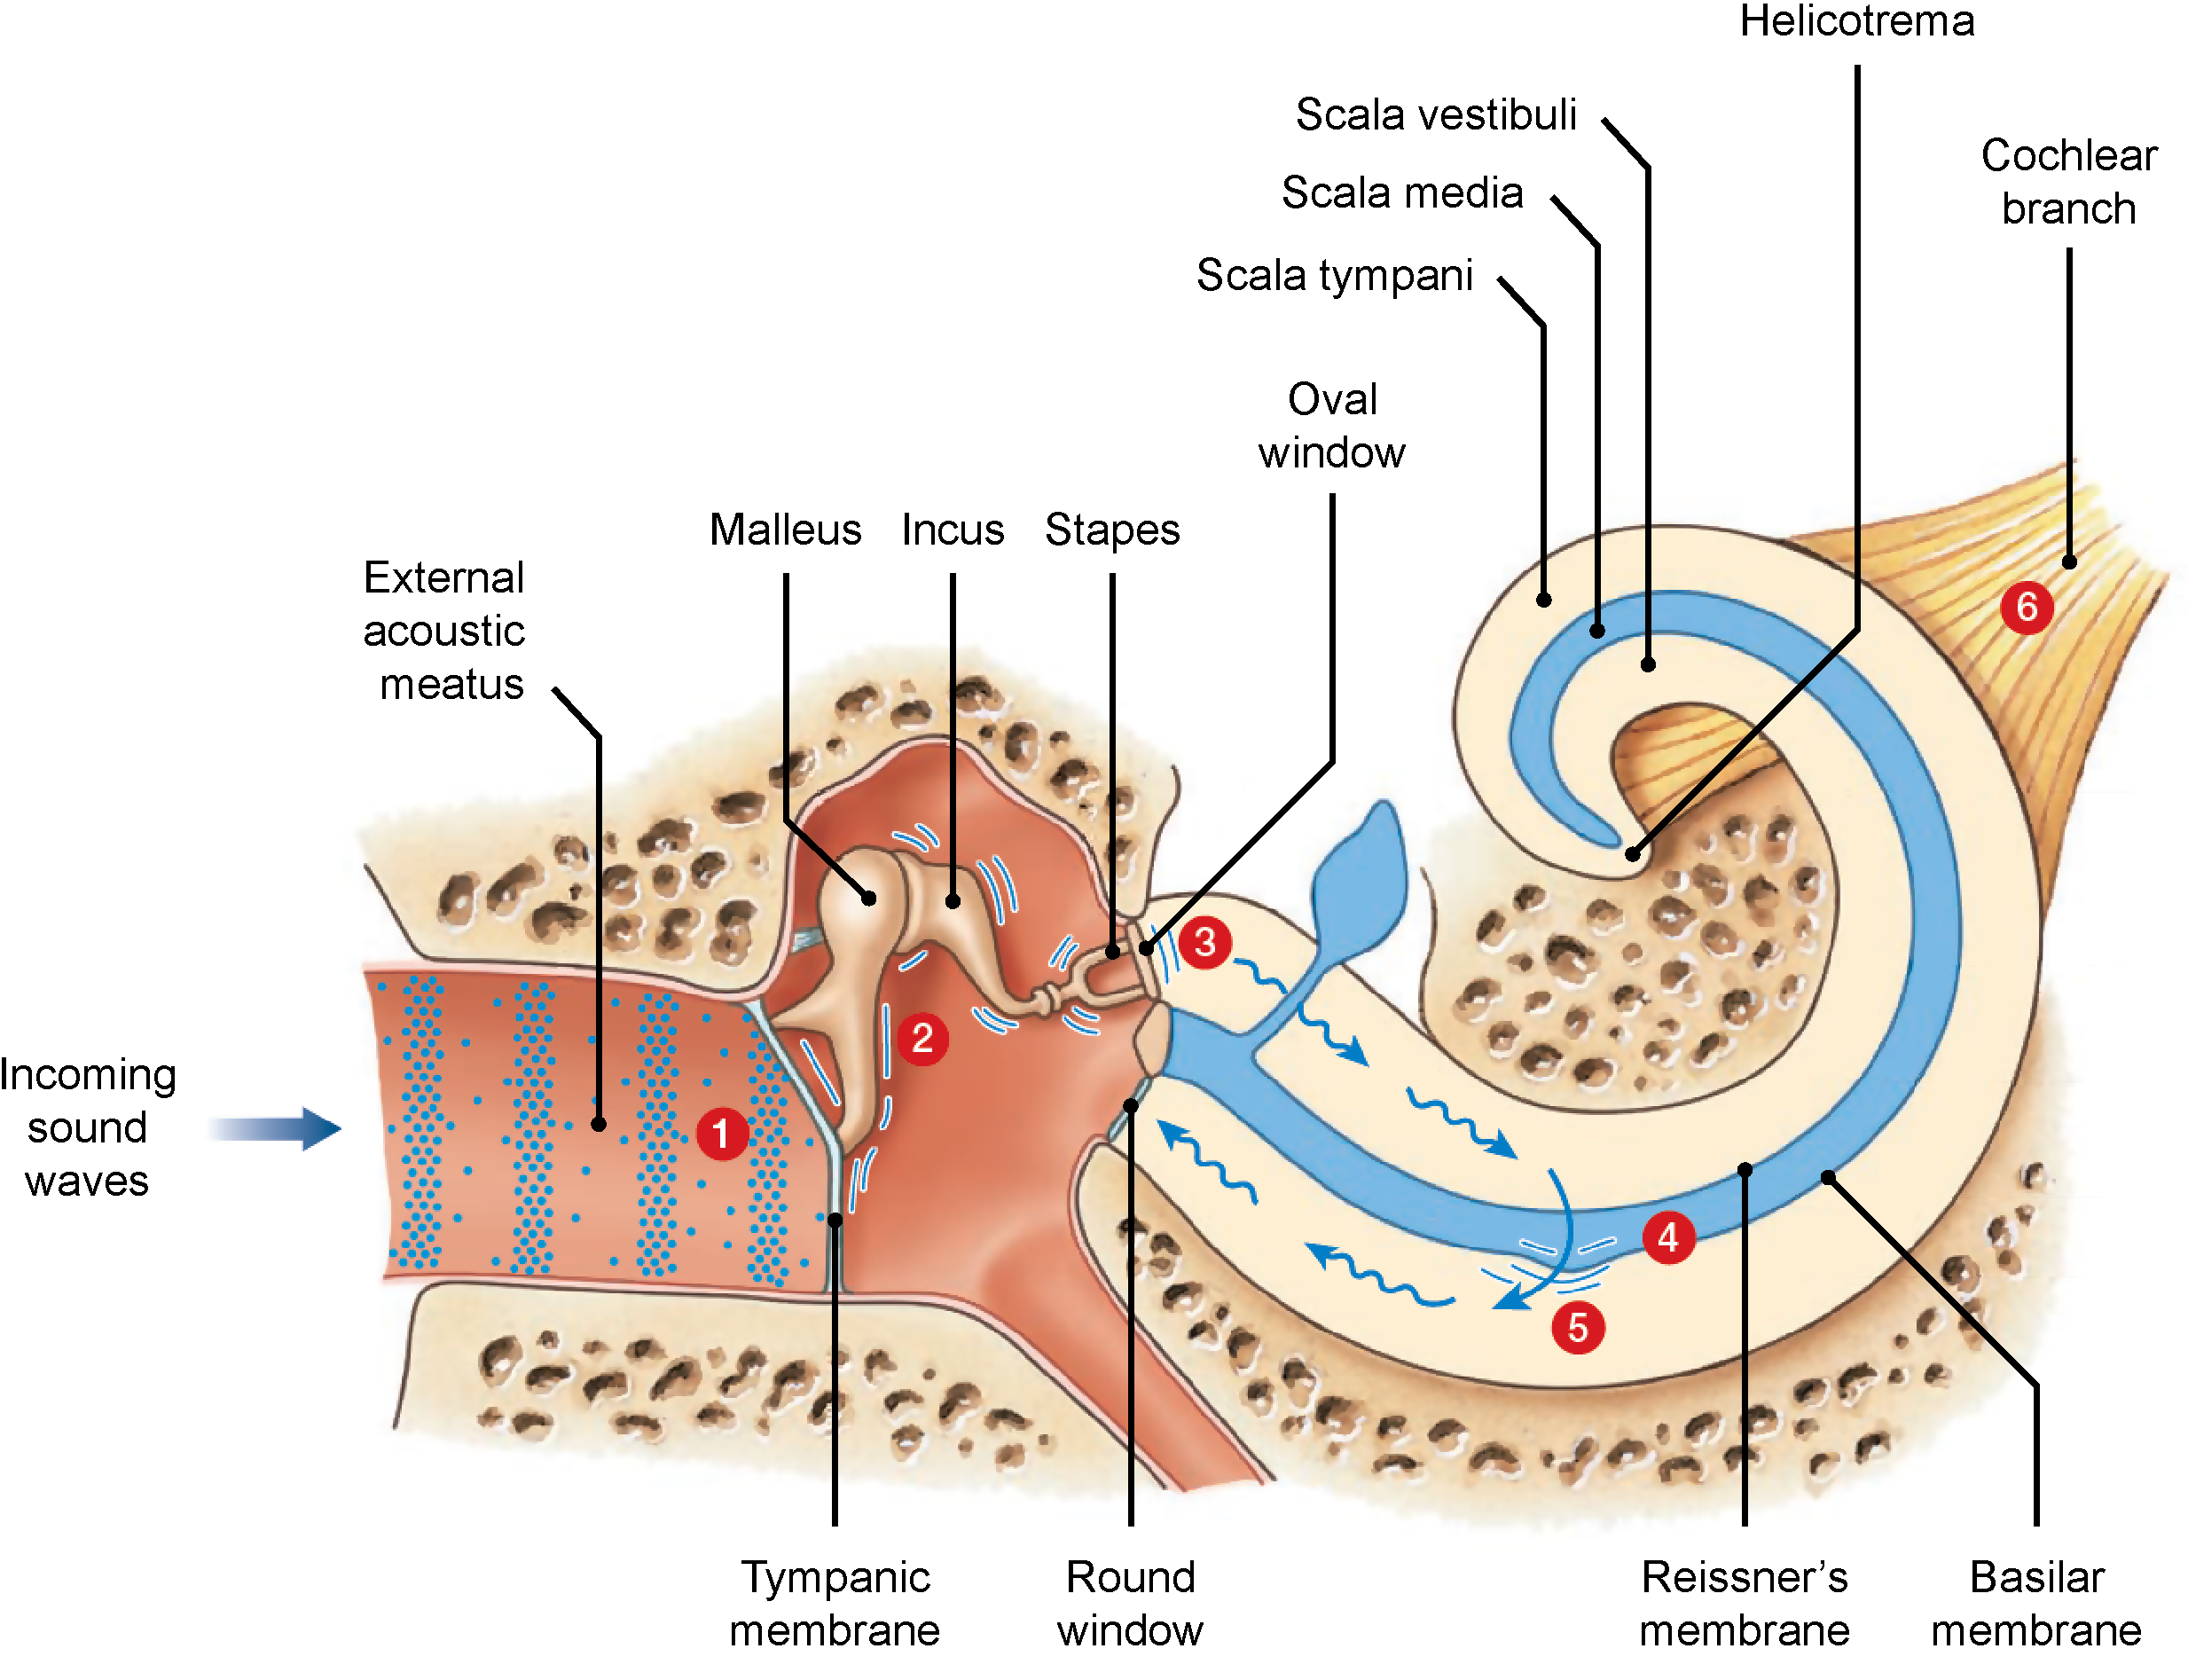
\includegraphics[width=\textwidth]{Background/normal_hearing.pdf}
	\caption[Sound wave propagation in the cochlea]{Sound wave propagation in the
	cochlea. Vibrations in the air are (1) received by the tympanic membrane, (2)
	transmitted via the ossicles to the oval window, and (3) travel up the scala
	vestibuli towards the helicotrema. For each frequency component, the
	travelling wave (4) peaks at a characteristic location along the cochlear
	partition and stimulates the corresponding hair cells, before (5) continuing
	via the scala tympani towards the round window, where the displacement is
	dissipated. Action potentials triggered by hair cell stimulation are (6) sent
	via the cochlear nerve to the auditory cortex for processing. (Image adapted
	from Martini~\etal\cite{martini2006}. Copyright \textcopyright{} 2006,
	Daryl Fox.)}
	\label{fig:travelling_wave}
\end{figure}

Sound waves travel up through the scala vestibuli to the helicotrema and return
via the scala tympani, generating a pressure gradient that distorts the organ of
Corti and the basilar membrane (together called the \emph{cochlear partition}).
Von B{\'e}k{\'e}sy~\cite{vonbekesy1960} showed that this \emph{travelling wave}
peaks at different locations along the basilar membrane due to its varying
stiffness, with higher frequencies peaking at the base and progressively lower
frequencies toward the apex as per Figure~\ref{fig:tonotopy}. As the cochlear
partition is deflected by the travelling wave, relative movement between the
tectorial membrane and the hair cells of the organ of Corti causes displacement
of the stereocilia. Displacement toward the tallest row opens ion channels in
the stereocilia, and the subsequent influx of cations depolarises the hair cell
(Figure~\ref{fig:stereocilia}). This in turn opens the calcium channels at the
base of the hair cell near the afferent nerve fibres, triggering the release of
neurotransmitters across the synapse and inducing action potentials in the
peripheral process of the auditory nerves. Displacement in the opposite
direction leads to hyperpolarisation. Neural excitation is discussed is more
detail in \S\ref{sect:neural_excitation}.

\begin{figure}
	\centering
	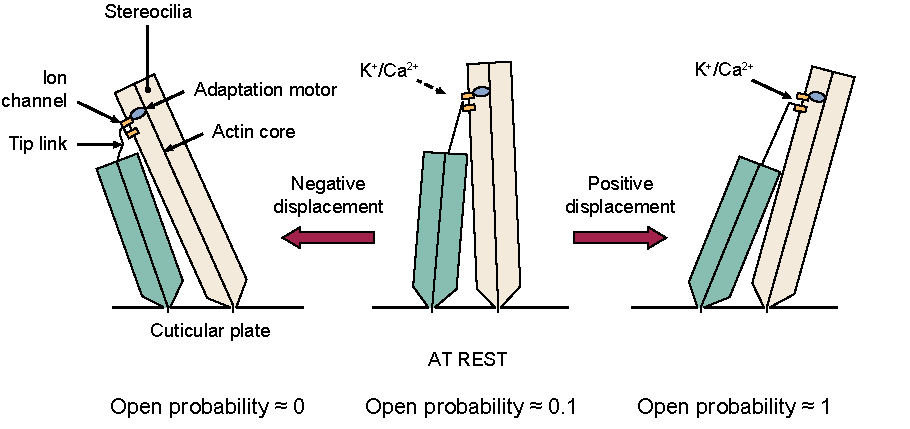
\includegraphics[width=15cm]{Background/stereocilia}
	\caption[Effect of stereocilia movement on ion channels]{Effect of stereocilia
	movement on ion channels. Displacement toward the tallest row stretches
	the spring-link tip links, opening the cation channels and leading to
	depolarisation of the hair cell. (Image adapted from
	Flint~\etal\cite{flint2010}. Copyright \textcopyright{} 2010, Mosby.)}
	\label{fig:stereocilia}
\end{figure}

According to the commonly accepted \emph{place theory} of pitch perception, hair
cells only respond to the frequency component which peaks at their particular
location along the basilar membrane. In this way, the cochlea can be thought of
as a mechanical Fourier transformer that directly extracts a spectral
representation from the sound stimulus~\cite{vonbekesy1960}. The correlation
between characteristic frequency and location (both along the cochlear partition
and in the auditory cortex) is termed the \emph{tonotopic organisation} of the
cochlea, and has been documented for several mammalian species by
Greenwood~\cite{greenwood1990}.

In the final stage, action potentials are relayed via N VIII to the auditory
cortex of the brain. It is there that the signals are decoded and interpreted,
giving rise to a conscious awareness of the original stimulus (i.e. sound
perception).

% ==============================================================================

\subsection{Hearing Loss}
\label{sect:hearing_loss}

Any reduction in the ability of an individual to perceive sound naturally is
known as hearing loss. There are two main categories: \emph{conductive hearing
loss} and \emph{sensorineural hearing loss}. A small proportion of affected
individuals suffer from \emph{mixed hearing loss}, where both of these cases are
exhibited.

Conductive hearing loss (CHL) occurs when there is a problem in the outer or
middle ear. Such conditions prevent vibrations in the air from being
mechanically transmitted through to the inner ear. Common causes of CHL include
obstruction of the external auditory meatus or of the auditory tube, thickening
or perforation of the tympanic membrane, bacterial or viral infections of the
middle ear, and fixation or decoupling of the auditory
ossicles~\cite{nadol1993,economics2006,flint2010}.

Sensorineural hearing loss (SHL) occurs when there is a problem with the
cochlea, the auditory nerve, or the auditory cortex. These locations are
downstream in the hearing chain, so SHL can manifest in individuals with a
normal outer and middle ear. The former is the most common and generally results
from damage to or degeneration of the hair cells in the organ of Corti. Common
causes of SHL include congenital malformations, exposure to excessive noise,
hair cell attrition due to aging (known as \emph{presbycusis}), and chemical
damage from smoking or medications~\cite{nadol1993,economics2006}. Disorders of
the inner ear vascular supply can also result in SHL~\cite{nadol1993}.

In either case, the degree of impairment can vary from negligible to complete
deafness. Scales are indicative but arbitrary, and can vary amongst authorities.
The classification system used by the World Health Organisation is shown in
Table~\ref{table:hearing_loss_classification}.

\section{Chapter Summary}

The cochlea is one part of the mammalian auditory pathway. It primarily consists
of three spiralling fluid chambers, known as the scalae vestibuli, media, and
tympani. These three chambers are separated by Reissner's membrane and the
cochlear partition (formed by the organ of Corti and basilar membrane)
respectively, and are bordered along the peripheral side by the spiral ligament
and stria vascularis. At the centre of the spiral path is the bony modiolus. The
cochlear nerve enters through the base of the modiolus and unravels to supply
the hair cells in the organ of Corti in a tonotopic manner. The major arteries
and veins of the cochlea also follow a modiolar path, with smaller radial
branches and capillary beds supplying the structures within. This is all
surrounded by the incredibly dense otic capsule, and is embedded in the petrous
portion of the temporal bone.

The overall structure is similar between humans and guinea pigs, but naturally
there are differences in geometry between species. Nonetheless, processes
leading to sound perception are the same. Sound entering a normal hearing
cochlea is picked up by the hair cells and transduced into a series of action
potentials that are interpreted by the brain. Unfortunately, this ability is
impaired in some individuals. For those with profound SHL due to hair cell
damage, the only successful treatment is a hearing prosthesis known as the
cochlear implant.

\clearpage

% ==============================================================================

% Page style from here up to References
	\pagestyle{fancy}
	\lhead{{\sffamily \MakeUppercase\leftmark}}
	\chead{}
	\rhead{{\sffamily \MakeUppercase\rightmark}}
	\lfoot{}
	\cfoot{{\sffamily \thepage}}
	\rfoot{}

\chapter{Literature Review}

% Textbox
\begin{center}
	\begin{tcolorbox}[title=\boxtitle]
		\begin{itemize}[leftmargin=*,labelindent=2ex,labelsep=1.5ex,itemsep=0pt,parsep=0pt]
		    \item What are cochlear implants?
			\item How does electrical stimulation compare to normal hearing?
			\item What is the state-of-the-art for bioelectric models of the cochlea?
			\item What are the outstanding issues that need to be addressed?
		\end{itemize}
	\end{tcolorbox}
\end{center}

\section{Cochlear Implants}
\label{sect:cochlear_implants}

Cochlear implants (CIs) are hearing prostheses that have been designed and
successfully used to treat severe to profound sensorineural hearing loss (SHL).
Although individuals with defective hair cells are unable to convert sound waves
into the corresponding neural excitation patterns~\cite{clark1996}, their
residual spiral ganglion cells and the corresponding neuronal axons are often
still healthy and functional~\cite{pfingst2011}. These tissues are therefore the
target of hearing restoration efforts. By injecting electric current into the
inner ear, CIs establish an electrochemical gradient in the cochlear tissues
that directly stimulates the afferent auditory nerve
fibres~\cite{nadol1988treatment,brown2001}, bypassing the defective hair cells.
The modular design of the nervous system, along with the plasticity of the brain
itself, enables these artificially induced neuronal impulses to be interpreted
as sound in much the same way as normal hearing~\cite{fallon2008}.

\subsection{Components and Function}

As shown in Figure~\ref{fig:CI_schematic}, most CI systems include both an
external unit (Figure~\ref{fig:nucleus_parts_ext}), which sits on the outside of
the head, and an internal unit (Figure~\ref{fig:nucleus_parts_int}), which is
surgically implanted under the scalp. The implant body is placed into a pocket
that is drilled into the mastoid bone, and the coiled electrode array is
inserted into the scala tympani of the cochlea (Figure~\ref{fig:CI_in_situ}).
The two parts communicate via transcutaneous induction, enabling the battery and
speech processor to be replaced or upgraded without revision surgery.

\begin{figure}[p]
	\centering
	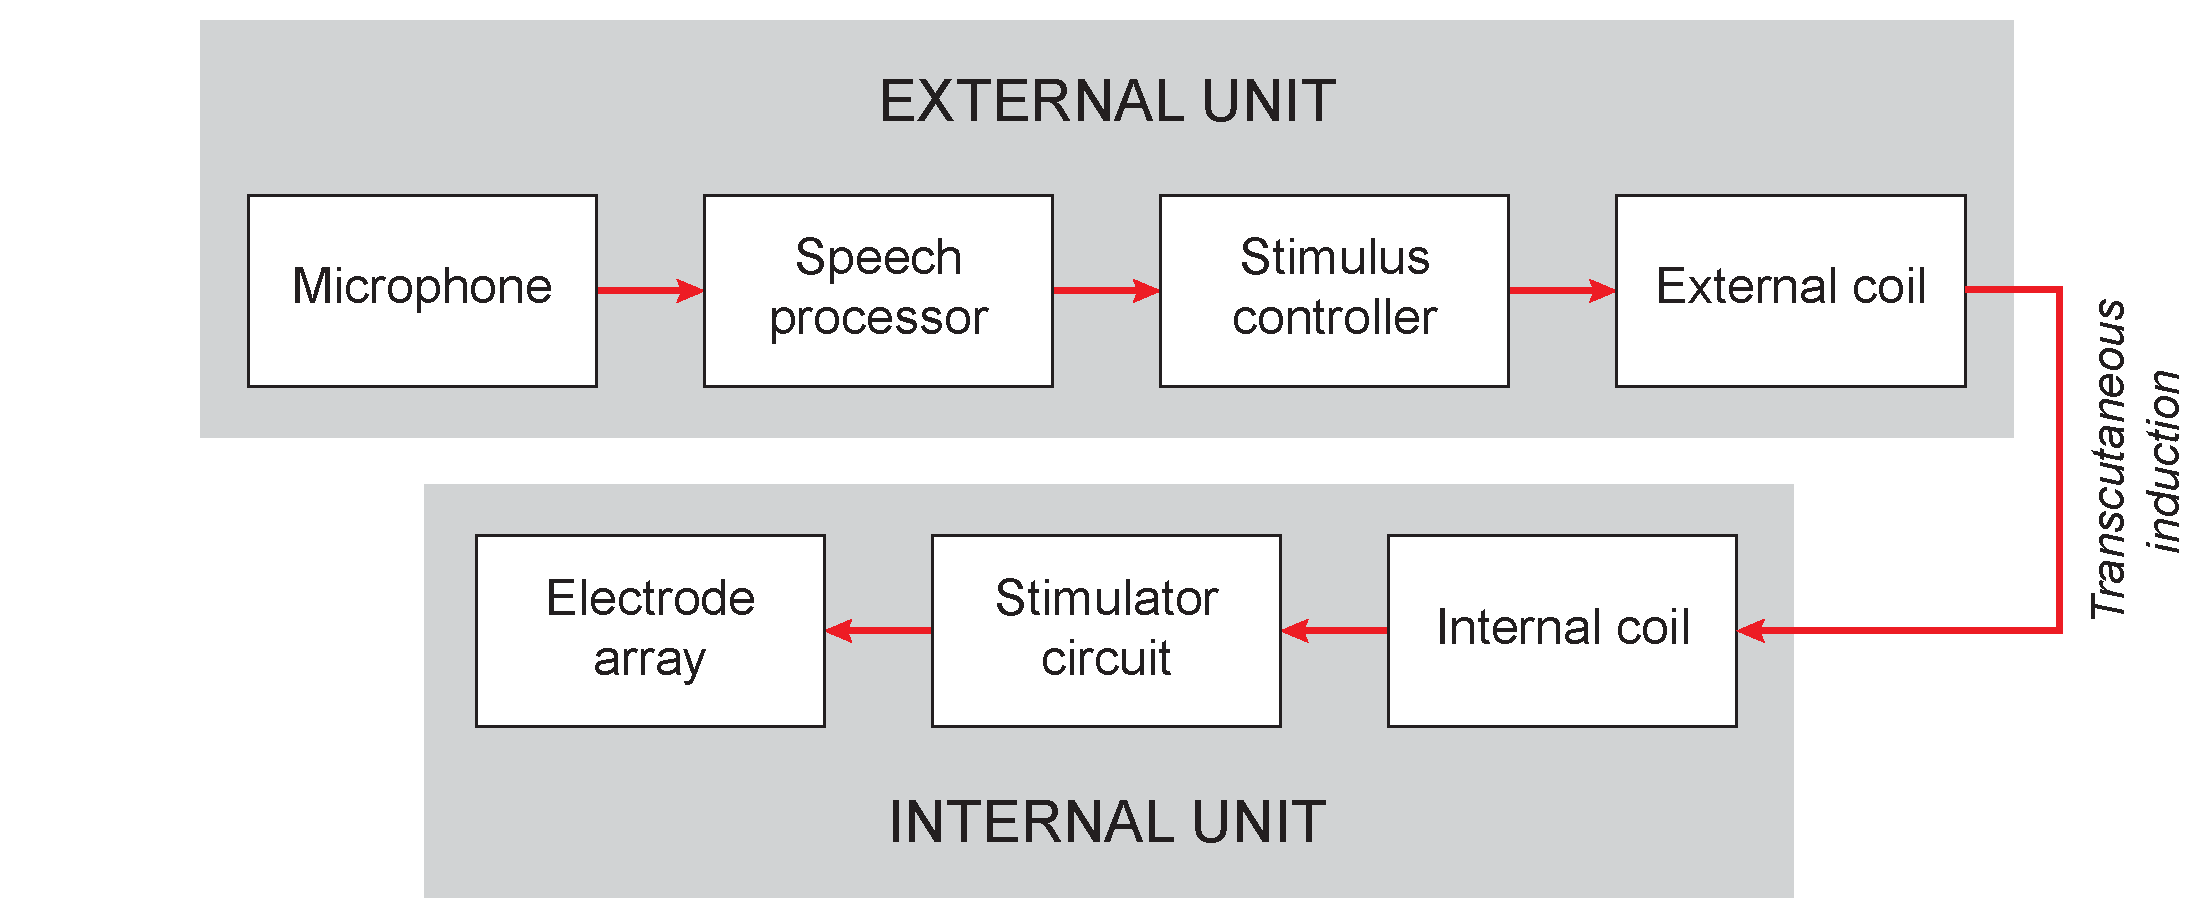
\includegraphics[width=14.5cm]{Background/implant_schematic.pdf}
	\caption[Schematic diagram of a cochlear implant system]{Schematic diagram of a
	cochlear implant system. (Adapted from Webster~\cite{webster1998}.)}
	\label{fig:CI_schematic}
\end{figure}

\begin{figure}[p]
    \centering
    \begin{subfigure}[t]{0.4\textwidth}
        \centering
        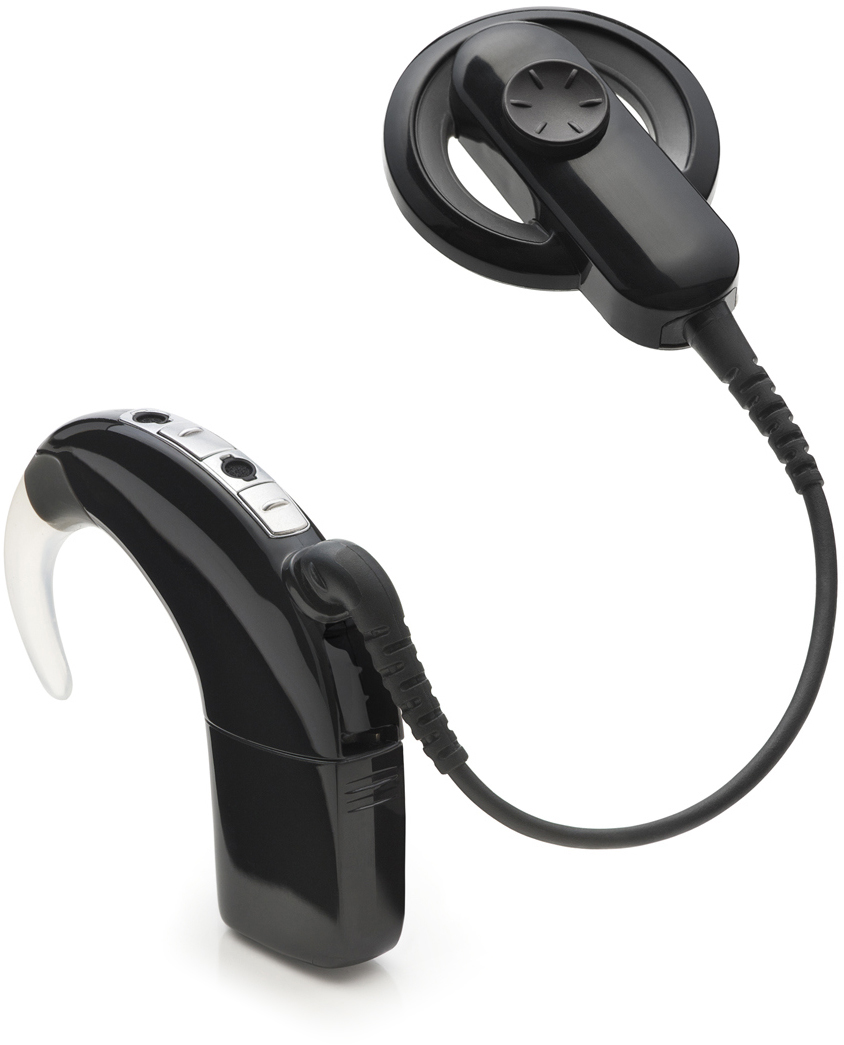
\includegraphics[height=7.5cm]{Background/CI_external_C920}
        \caption{ }
        \label{fig:nucleus_parts_ext}
    \end{subfigure}
    \hspace{1cm}
    \begin{subfigure}[t]{0.4\textwidth}
        \centering
        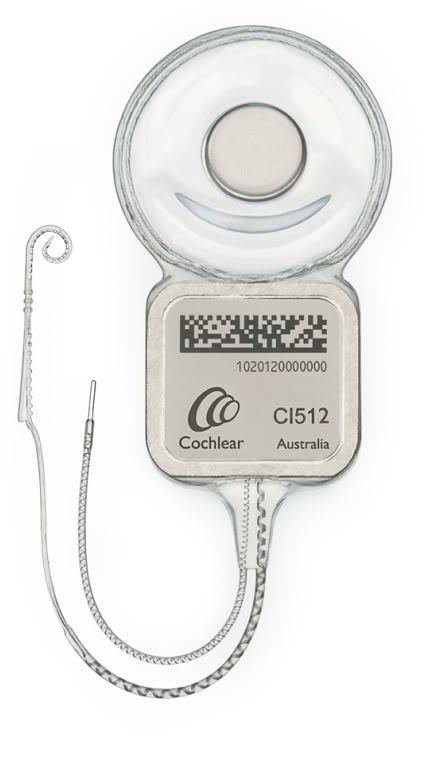
\includegraphics[height=7.5cm]{Background/CI_internal_CI512}
        \caption{ }
        \label{fig:nucleus_parts_int}
    \end{subfigure}
    
	\caption[The Nucleus 6 cochlear implant system by Cochlear Limited]{The Nucleus
	6 cochlear implant system by Cochlear Limited. (a) The external behind-the-ear
	unit, housing the battery, microphone, speech processor, and stimulus
	controller tethered to the external coil. (b) The cochlear implant proper,
	consisting of the internal coil, stimulator circuitry, return electrodes, and
	intracochlear electrode array. The external and internal coils are
	aligned using magnets. (Source:	Cochlear Limited.)}
	\label{fig:nucleus_parts}
\end{figure}

\begin{figure}
	\centering
	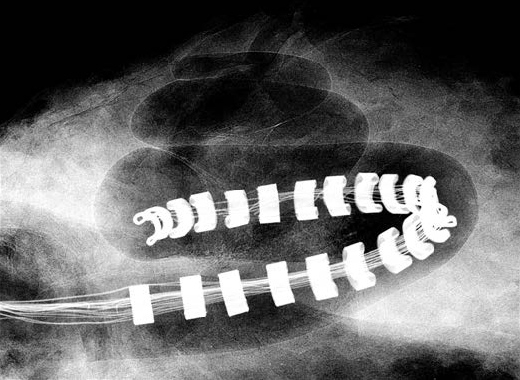
\includegraphics[height=5.8cm]{Background/CI_phase-contrast_x-ray}
	\caption[Phase-contrast x-ray image of an intracochlear electrode array
	\insitu]{Phase-contrast x-ray image of an intracochlear electrode array
	\insitu. Note how the half-banded electrode pads in this design face towards
	the modiolus. (Source: Xu~\cite{xu2001}. Copyright \textcopyright{} 2001,
	Wolters Kluwer.)}
	\label{fig:CI_in_situ}
\end{figure} 

The system mimics the processes that occur during normal hearing. Sound waves
are detected using a microphone on the external unit, fulfilling the role of the
tympanic membrane. These signals are sent to a speech processor, which uses a
combination of Fourier transformations, band-pass filters, and envelope
detection algorithms to extract spectral and temporal auditory information from
the waveform. In essence, the speech processor replicates the mechanical
transduction of the cochlea using electronics. Over the years, many different
speech processing algorithms have been developed, with the aim of extracting and
presenting as many useful cues to implant recipients as possible.
Louizou~\cite{loizou1998} provides a good summary of the developments in this
area.

The stimulus controller then maps each frequency band to the corresponding
electrode pad in the intracochlear array, adjusts each signal to meet
patient-specific current thresholds that are determined during a post-operation
training phase, and encodes these stimulus parameters for each channel. These
signals, along with power, are sent via the induction link to the implanted
receiver-stimulator circuitry, which in turn directs the current pulses to the
appropriate electrode pad along the intracochlear
array~\cite{webster1998,clark1996}. Since the array follows the spiral path of
the cochlea, different pads inject current pulses at different locations
corresponding to the tonotopic organisation of the nerve fibres (see, for
example, Figure~\ref{fig:pitch_place}). This allows the CI to elicit percepts
for a wide range of targeted frequencies as required for effective speech
recognition~\cite{eddington1977,busby1994,clark2013}.

\begin{figure}
	\centering
	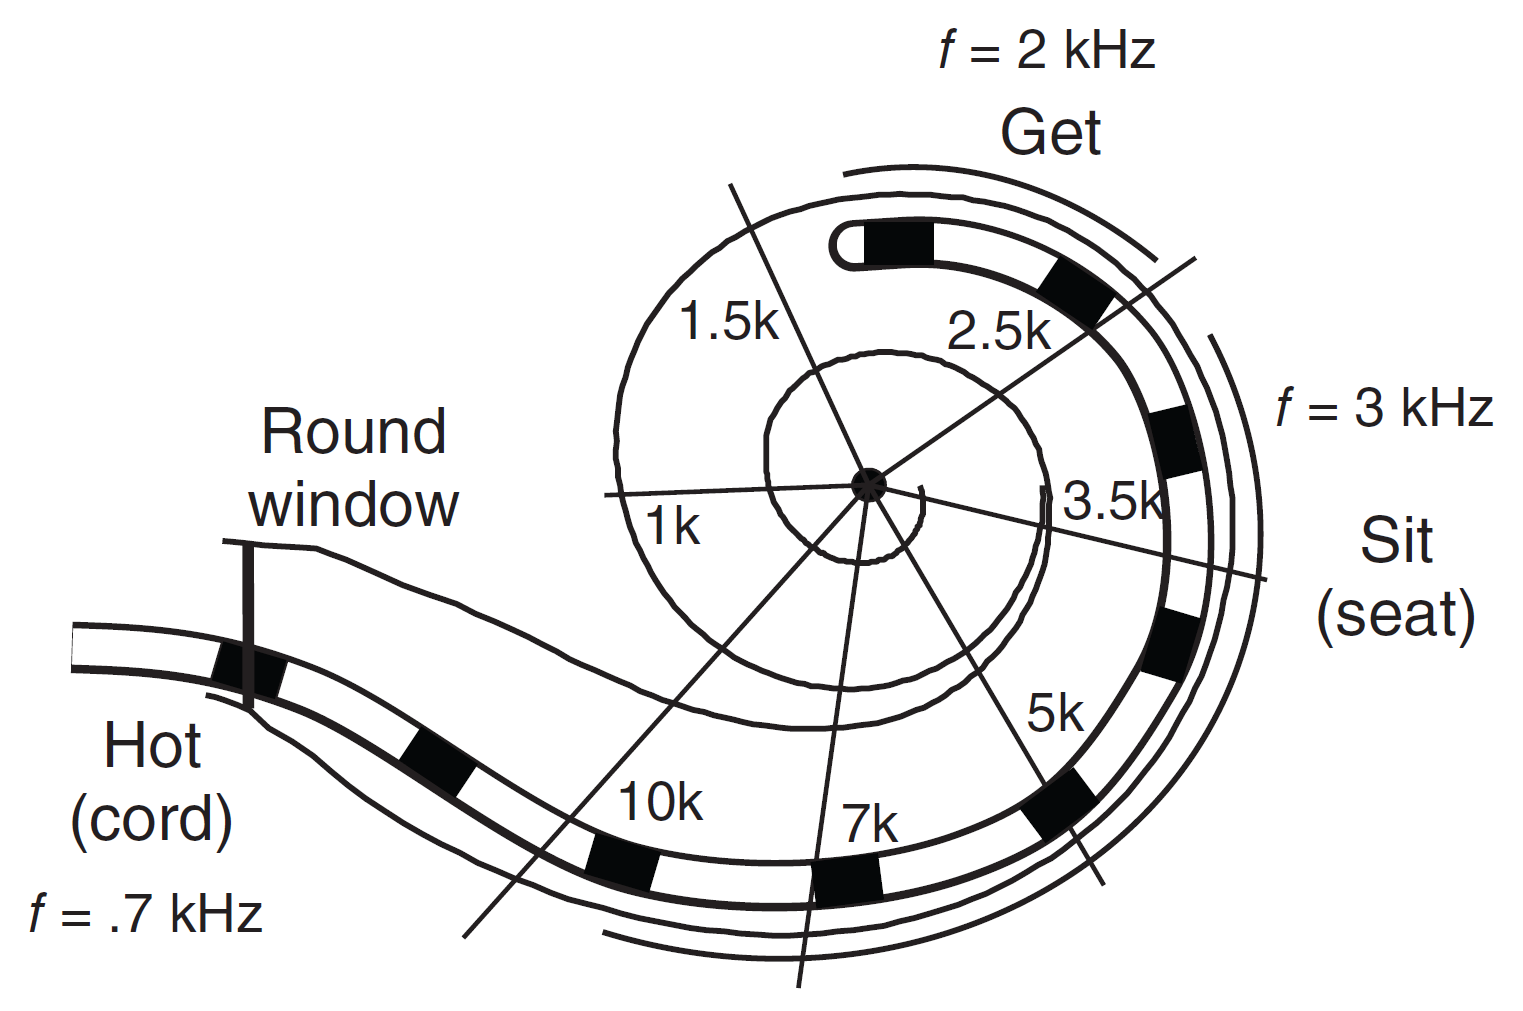
\includegraphics[height=6cm]{Background/pitch_place}
	\caption[Correlation between electrode location and perceived
	frequency]{Correlation between intracochlear electrode location and perceived
	frequency as observed in Rodney Saunders, the first cochlear implant recipient.
	Note the similarities with Figure~\ref{fig:tonotopy}. (Source:
	Clark~\cite{clark2013}. Copyright \textcopyright{} 2013, Macmillan Publishers
	Limited.)}
	\label{fig:pitch_place}
\end{figure}

\subsection{Stimulation Mechanics}

Although the process of charge injection sounds relatively straightforward, the
details of actually implementing such a system are quite complex. Two aspects
that are particularly relevant to this thesis are discussed briefly below.

\subsubsection{Charge Balance}
\label{sect:charge_balance}
% Talk about different stimulation modes and rates, pulse width vs pulses per
% second (Wilson paper),

Metals are \emph{electronic conductors}, i.e. the particles responsible for
carrying charge are electrons; in contrast, biological tissues are
\emph{electrolytic conductors}---the charge carriers are
ions~\cite{webster1998,grimnes2000}. Since metals contain no free ions and the
inner ear fluids have no free electrons, intracochlear electrodes must transduce
an electronic current into an ionic current to effect charge injection across
the electrode-tissue interface. This is accomplished through chemical reactions
at the interface~\cite{webster1998}.

% Talk about water window?
The typical surface reactions for platinum electrodes are listed in
Table~\ref{table:interface_reactions}. At the time of writing, platinum is the
preferred material for use in intracochlear electrodes because its inertness
makes it unlikely to oxidise and dissolve into the \invivo{}
environment~\cite{merrill2005}---a crucial attribute for safe, long-term
electrical stimulation. The chemical stability of the electrode alone is,
however, not a sufficient condition for safety.

\begin{table}
	\centering
	\sffamily
	\small
	
	\caption[Surface reactions at the electrode-tissue interface]{Surface reactions
	at the electrode-tissue interface, in order of increasing potential.
	(Compiled from various sources~\cite{brummer1977,merrill2005}.)}
	\label{table:interface_reactions}
	
	\begin{subtable}[t]{0.8\textwidth}
        \caption{Oxidation reactions.}
        \label{table:interface_reactions_ox}

        \centering
        
        \begin{tabularx}{\textwidth}{p{3.5cm} X}
		\toprule
		\textbf{Reaction}		& \textbf{Equation} \\
		\midrule
		
		Oxygen plating			& \ce{Pt + 2[OH]-} $ \rightleftharpoons $ \ce{PtO + H2O	+ 2e^-} \\
		Oxygen evolution		& \ce{4[OH]^-} $ \rightleftharpoons $ \ce{O2 + 2H2O + 4e^-} \\
		Oxidation of organics	& \ce{CH3CH2OH + 2[OH]^-} $ \rightleftharpoons $ \ce{CH3CHO + 2H2O + 2e^-} \\
		\tableindent\textit{(example)} & \\
		Platinum dissolution 	& \ce{Pt + 4Cl^-} $ \rightleftharpoons $ \ce{[PtCl4]^{2-} + 2e^-} \\
		Chlorine evolution		& \ce{2Cl^-} $ \rightleftharpoons $ \ce{Cl2 + 2e^-} \\
		
		\bottomrule
		\end{tabularx}
		
    \end{subtable}
    
    \vspace{10pt}
    
    \begin{subtable}[t]{0.8\textwidth}
        \caption{Reduction reactions.}
        \label{table:interface_reactions_red}

        \centering
        
        \begin{tabularx}{\textwidth}{p{3.5cm} X}
		\toprule
		\textbf{Reaction}		& \textbf{Equation} \\
		\midrule
		
		Oxygen reduction		& \ce{1/2O2 + H2O} $ \rightleftharpoons $ \ce{H2O2} \\
		Hydrogen plating		& \ce{Pt + H^+ + e^-} $ \rightleftharpoons $ \ce{PtH} \\
		Hydrogen evolution		& \ce{2H^+ + 2e^-} $ \rightleftharpoons $ \ce{H2} \\
		
		\bottomrule
		\end{tabularx}
		
    \end{subtable}
	
\end{table}

Consider electric current that is applied in a single direction, say from the
electrode to the inner ear fluids. With time, this current will deliver a net
charge that favours oxidation reactions, and the products of these reactions
will accumulate and diffuse away from the electrode-tissue interface due to
concentration gradients~\cite{grimnes2000}. These products, such as the
evolution of chlorine gas \invivo{} (Table~\ref{table:interface_reactions_ox}),
may be harmful to the cochlear
tissues~\cite{lilly1955,brummer1977,shepherd1991}.

To prevent such a situation, current is typically delivered as charge-balanced
biphasic pulses~\cite{cogan2008}, an example of which is illustrated in
Figure~\ref{fig:biphasic_pulse}. The first phase of a biphasic input is
responsible for neuronal recruitment~\cite{ranck1975,reilly1998,zeng2004}. The
second phase, which occurs during the refractory period of the stimulated
neurons, serves to neutralise the overall charge and reverse any reactions
induced during the first phase. Most electrical stimulation systems use
cathodic-first pulses because cathodic stimulation produces a higher
depolarisation peak than anodic stimulation~\cite{ranck1975} and therefore
requires less current to reach the threshold for excitation.

\begin{figure}
	\centering
	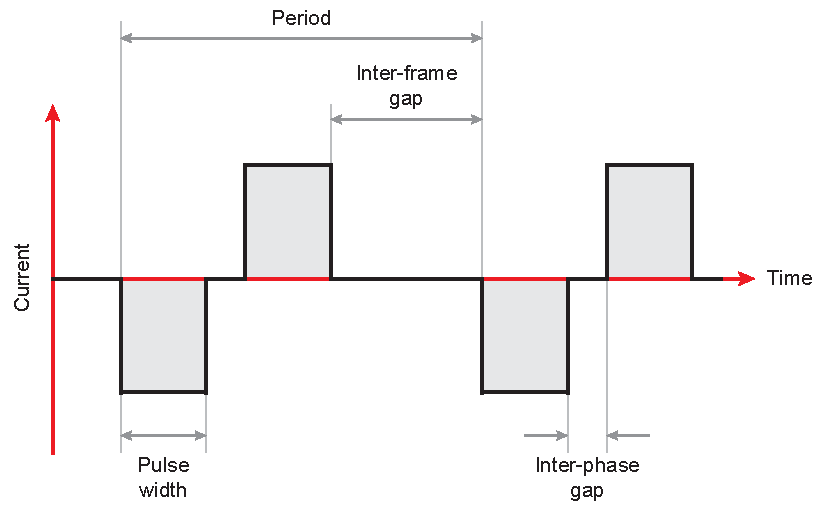
\includegraphics[height=8cm]{Background/biphasic_pulse}
	\caption[Charge-balanced, cathodic-first biphasic pulses]{Charge-balanced,
	cathodic-first biphasic pulses, typically used in electrical stimulation. The
	overall period of a pulse can be divided into subtimings such as the pulse
	width, inter-phase gap, and inter-frame gap as labelled in the diagram. Charge
	delivered during each phase (represented by the shaded areas) should be equal.}
	\label{fig:biphasic_pulse}
\end{figure}

CIs typically use a constant current level for each pulse to simplify the
balancing of electric charge (Figure~\ref{fig:const_current_waveform}). The
phases are usually symmetric (i.e. they have the same amplitude and pulse
width), but it is possible to use asymmetric pulses so long as charge balance is
maintained~\cite{cogan2008}. Constant voltage pulses
(Figure~\ref{fig:const_voltage_waveform}) may also be used, but are not common
in practice. The electric potential at the stimulating electrode varies over
time when constant current pulses are used due to the capacitive effects of the
electric double layer at the
interface~\cite{geddes1972,cobbold1974,grimnes2000}. Care must be taken to
ensure that the total potential does not enter the range that induces
irreversible reactions.

\begin{figure}
	\centering
	\begin{subfigure}[t]{0.6\textwidth}
        \centering
        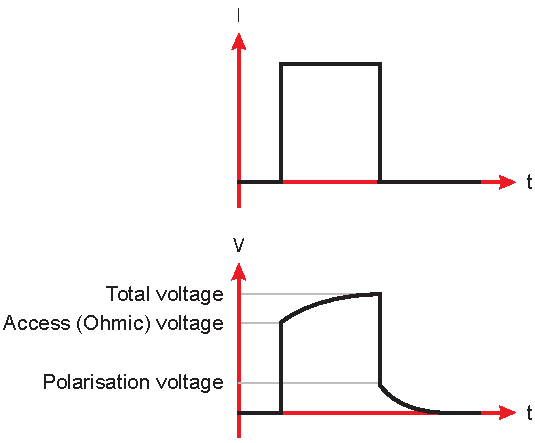
\includegraphics[height=7.2cm]{Background/constant_current}
		\captionsetup{margin={3.65cm,0cm}}
        \caption{ }
        \label{fig:const_current_waveform}
    \end{subfigure}
    ~
    \begin{subfigure}[t]{0.375\textwidth}
        \centering
        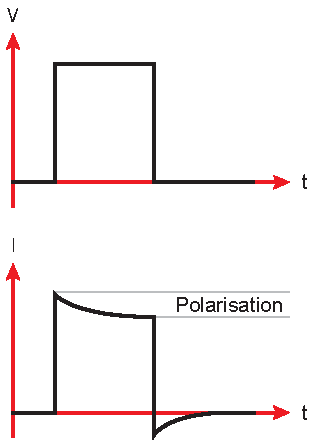
\includegraphics[height=7.2cm]{Background/constant_voltage}
        \captionsetup{margin={-0.05cm,0cm}}
        \caption{ }
        \label{fig:const_voltage_waveform}
    \end{subfigure}
    
	\caption[Constant current versus constant voltage waveforms]{Current and
	voltage waveforms for (a) constant current pulses, and (b) constant voltage
	pulses. Constant current pulses are generally preferred because they make it
	easier to ensure zero net charge injection. The access voltage is the same at
	both the leading and trailing edges of the pulse. (Adapted from
	Webster~\cite{webster1998}.)}
	\label{fig:current_voltage_waveforms}
\end{figure}

\subsubsection{Electrode Configurations}
\label{sect:electrode_configs}

Most CI systems in use today have multiple channels and up to two dozen
independent electrodes~\cite{clark2006}. Cochlear Limited's Contour Advance, for
example, has 22 half-banded platinum contacts along the intracochlear array, a
platinum ball-shaped electrode that is tethered to the implant unit, and the
exposed titanium casing around the stimulator circuitry, which effectively
serves as a plate electrode. Since a source-sink configuration can be set up
between any subset of these electrodes, there are a variety of different
combinations that may be employed~\cite{busby1994}, some of which are
illustrated schematically in Figure~\ref{fig:stim_modes}.

\begin{figure}
	\centering
	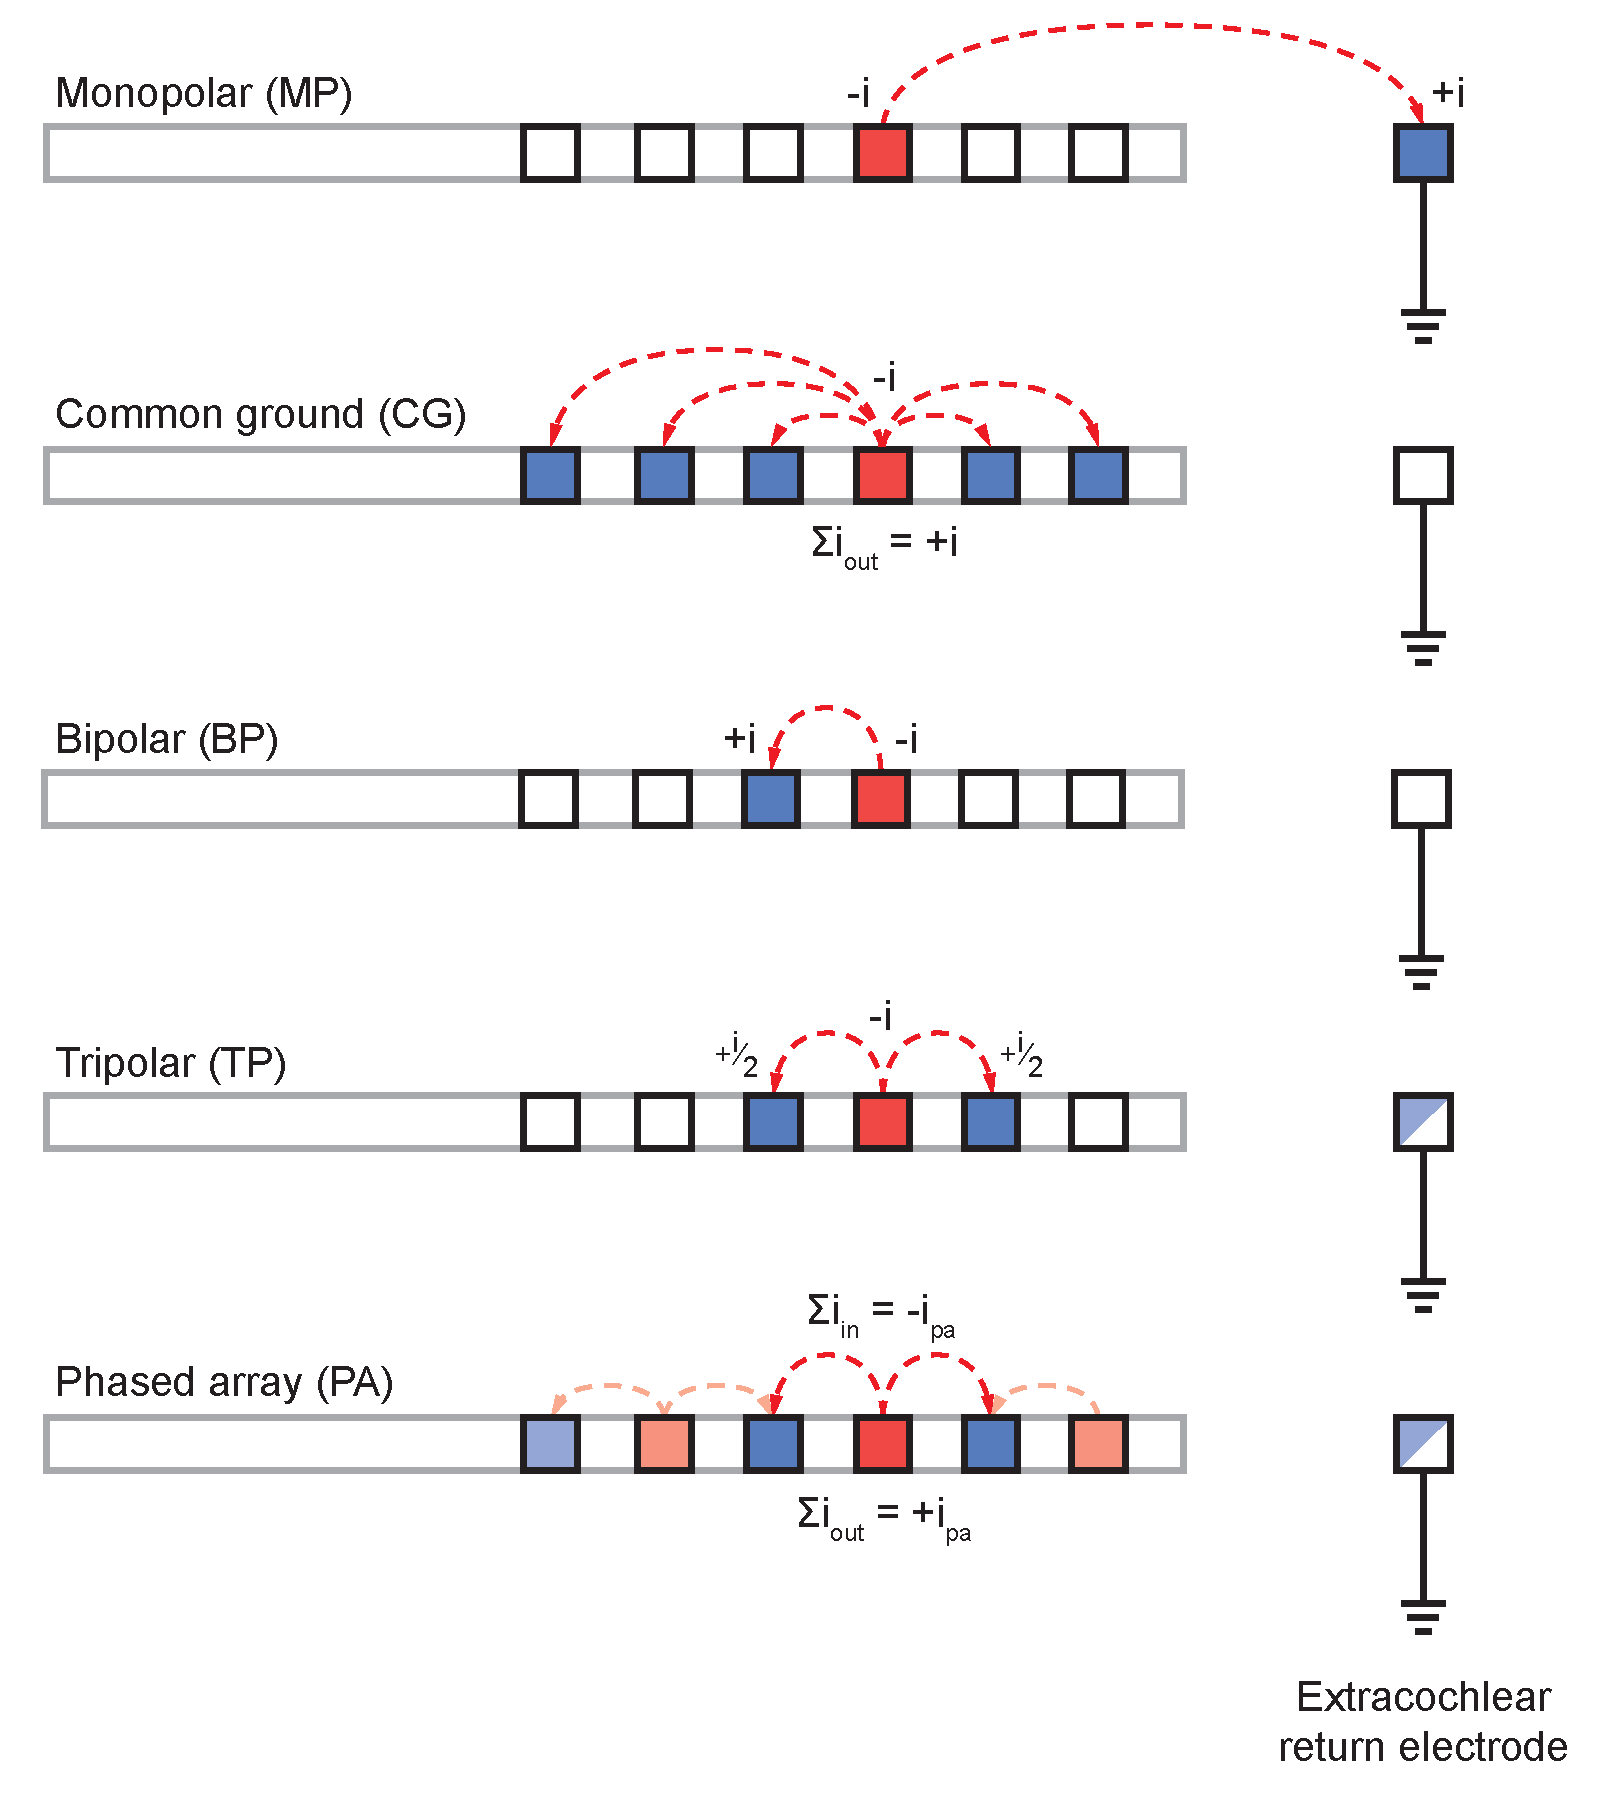
\includegraphics[width=12.8cm]{Background/electrode_config.pdf}
	\caption[Modes of stimulation]{Modes of stimulation for a cochlear implant.
	MP stimulation is the most common mode used in implant recipients. Note that
	the extracochlear electrode may be used in TP and PA stimulation modes.
	Different configurations produce different current paths in the cochlear
	volume, and the resulting perception of sound can differ in many ways.}
	\label{fig:stim_modes}
\end{figure}

\emph{Monopolar} (MP) stimulation is the most common configuration used in
contemporary CIs. Here, current is only injected at one of the intracochlear
electrodes, and returns via the bodily tissues to one or both of the
extracochlear electrodes. This mode of stimulation tends to yield the lowest
thresholds~\cite{busby1994} (i.e. the minimum current level required for the CI
recipient to perceive sound) because the injected current spreads out from the
source electrode, but conversely, the current is also the least
focused~\cite{bonham2008}, stimulating neurons over a relatively wide band of
frequencies in the process~\cite{kral1998,vandenhonert2007}.

Stimulating a narrower band of neurons is an important goal because it enables
finer pitch discrimination in CI recipients~\cite{kral1998,vandenhonert2007}.
One way to achieve this is to use \emph{common ground} (CG) stimulation, where
the non-stimulating electrodes are used together as a single return path instead
of the extracochlear electrode~\cite{busby1994}. In a \emph{bipolar} (BP)
configuration, two intracochlear electrodes are used as the source and the sink.
The two electrodes are typically adjacent, but may also be separated by one or
two pads (known as BP+1 and BP+2, respectively). BP stimulation was often used
during the early phases of multielectrode CI development because, at least in a
homogeneous material, injected current would flow more or less directly between
the two electrodes, limiting the spread of excitation~\cite{black1980,kral1998}.
A variation of BP, called \emph{tripolar} (TP) stimulation, splits the return
path between both adjacent flanking electrodes and, if desired, the
extracochlear electrode, generating a more symmetric field like that of MP
stimulation but with less current spread~\cite{kral1998,busby1994}.
Recent research efforts have looked at \emph{phased array} (PA)
stimulation~\cite{vandenhonert2007,frijns2011,george2014}, also known as
multipolar stimulation in some texts. In this mode, opposing currents are
applied at all electrodes, with weightings based on the inverted transimpedance
matrix along the array to yield a resultant voltage profile that is zero at all
but the stimulating electrode(s)~\cite{vandenhonert2007}.

As with other design decisions, there are costs associated with the use of more
focused stimulation modes. \textit{Ceteris paribus}, the trade-off is higher
power draw when generating auditory percepts at any given level of
loudness~\cite{vandenhonert2007,saba2012}. In addition, there may be no
perceptual benefit in using more focused modes if the residual spiral ganglion
cell bodies in the region of the targeted frequency band have already
degenerated~\cite{pfingst2011}.

\subsection{Efficacy and Unsolved Challenges}

CI stimulation has come a long way since the first recipient was
implanted~\cite{black1980,clark2013}. Clinical reviews, such as those by Nadol
and Eddington~\cite{nadol1988treatment} and Clark~\cite{clark1996}, have shown
significant progress in the restoration of hearing perception. Economic
reports~\cite{economics2006} have also noted their benefit to the wider society
due to flow on effects such as increased productivity and wellbeing in CI
recipients. Indeed, the mere fact that the industry itself exists is a testament
to the success of the CI in fulfilling its mandate.

Nonetheless, there are several scenarios for which CIs can still be
significantly improved. Firstly, noisy environments are commonly encountered in
daily life and present an ongoing challenge for CI recipients because the noise
masks individual sound signals, making it difficult to isolate the desired
source~\cite{stickney2004,gfeller2007}. Secondly, music perception has been
found to be less enjoyable following implantation due to inadequate pitch and
timbre perception~\cite{leal2003,mcdermott2004,sucher2007}. Thirdly, although
the CI is well tuned for English speakers, those who speak tonal languages miss
out on a lot of semantic
information~\cite{ciocca2002,xu2002,wei2004,vandenhonert2007}. Many have called
for or assumed that better speech processing techniques will overcome these
challenges because most of the improvements in patient outcomes have thus far
stemmed from research in that
area~\cite{skinner1994,loizou1998,micco2006,vandenhonert2007}, but despite the
merits of more sophisticated algorithms, updates in speech processing have not
resulted in the desired level of clinical advancement for many years
now~\cite{seligman2004,zeng2008}.

Considering that the mechanism ultimately responsible for auditory nerve
stimulation is the \invivo{} current distribution, it would appear that the
bottleneck of information transfer in CI systems lies with the implanted unit,
specifically with existing designs of the intracochlear electrode
array~\cite{clark2008,clark2013}. Given the difficulties of obtaining and
visualising such information using \invivo{} and \invitro{} experiments alone, a
detailed \insilico{} electroanatomical map of CI induced current flows would be
valuable for furthering our understanding of the cochlea's electrical
behaviour~\cite{spelman1982,girzon1987,suesserman1993,frijns1995,schimpf1998,
micco2006,whiten2007,potratz2010}. An accurate and well-validated model has the
potential to reveal methods for achieving more precise spatial control of the
electric field generated by the CI, as well as other benefits such as lower
power consumption. New intracochlear electrode array designs may also be
virtually prototyped and tested for efficacy before any physical assets are
requested~\cite{zeng2004}, reducing the overall cost of development while
optimising implant design and performance.

% ==============================================================================

\section{Bioelectric Modelling}

\subsection{Expected Physics}
\label{sect:expected_physics}

At a fundamental level, the CI is just like any other system of electrical
interactions. The flow of electric current from the stimulating electrode to the
return electrode and the corresponding fields and fluxes are fully described by
\emph{Maxwell's equations}~\cite{maxwell1865}. They can be written in
differential form as:
\begin{eqnarray}
	\nabla \cdot \vec{E} &=& \frac{\rho}{\epsilon_0}
		\label{eqn:maxwell_1} \\
	\nabla \cdot \vec{B} &=& 0 \phantom{\frac{1}{1}}\\
	\nabla \times \vec{E} &=& -	\frac{\partial \vec{B}}{\partial t} \\
	\nabla \times \vec{B} &=& \mu_{0}\vec{J} +
		\mu_{0}\epsilon_{0}\frac{\partial \vec{E}}{\partial t}
		\label{eqn:maxwell_4}
\end{eqnarray}
where $ \nabla $ is the gradient operator, $ \vec{E} $ is the electric field,
$ \vec{B} $ is the magnetic field, $ \rho $ is electric charge density, $
\vec{J} $ is electric current density, $ \epsilon_{0} $ is the permittivity of
free space, $ \mu_{0} $ is the permeability of free space, and $ t $ is time.
Equations~\ref{eqn:maxwell_1}--\ref{eqn:maxwell_4} are also known as Gauss's
law for electricity, Gauss's law for magnetism, Faraday's law of induction, and
Amp{\`e}re's circuit law with Maxwell's addition, respectively.

In a CI system, these field quantities are determined by three main factors: the
locations of the electrodes, the electric properties of the cochlear tissues,
and the magnitude and shape of the injected current pulse. The current pulse is
under the control of the device itself and is therefore a well-known input
quantity. The other factors are more difficult to quantify, but some insight can
be gained from first principles.

In a homogeneous and isotropic cell with end-plate electrodes, the induced
electric field is uniformly distributed
(Figure~\ref{fig:end_electrodes_uniform}). Consider now a cell that is not
homogeneous, but instead contains a second material of different resistivity to
the first. In this case, the flux lines would exhibit some distortion because
the newly introduced material changes the shape of the electric
field~\cite{baker1989}, as shown in Figure~\ref{fig:end_electrodes_distorted}.
Relatively conductive tissues tend to funnel current flow, while those that are
relatively insulating are avoided as the current seeks out the path of least
resistance. The larger the difference in resistivity between the two materials,
the more distortion that can be expected.

\begin{figure}[p]
	\centering
	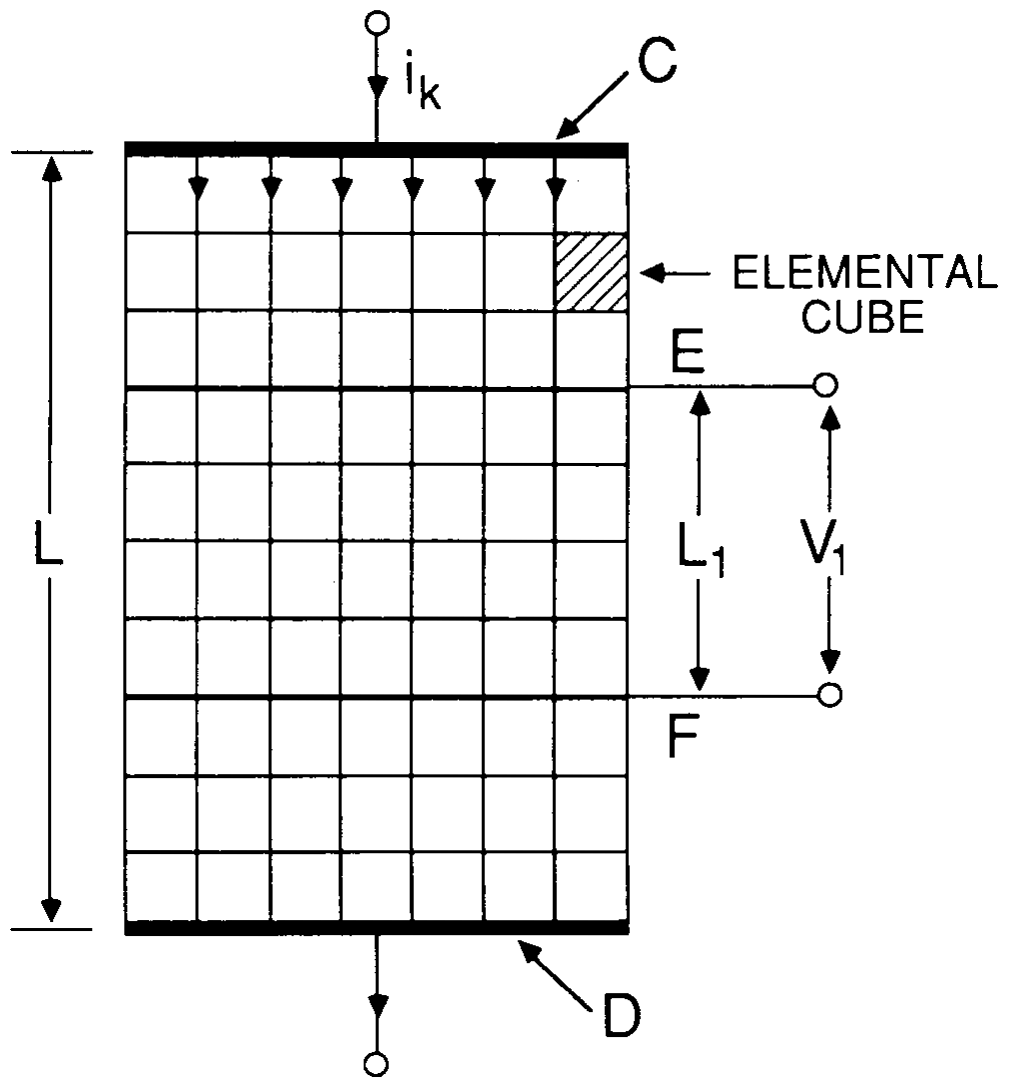
\includegraphics[height=5.6cm]{Background/end_electrodes_uniform}
	\caption[Uniform flux lines in a homogeneous isotropic cell]{Uniform flux lines
	in a homogeneous isotropic cell. (Source: Baker~\cite{baker1989}. Copyright
	\textcopyright{} 1989, IEEE.)}
	\label{fig:end_electrodes_uniform}
\end{figure}

\begin{figure}[p]
	\centering
	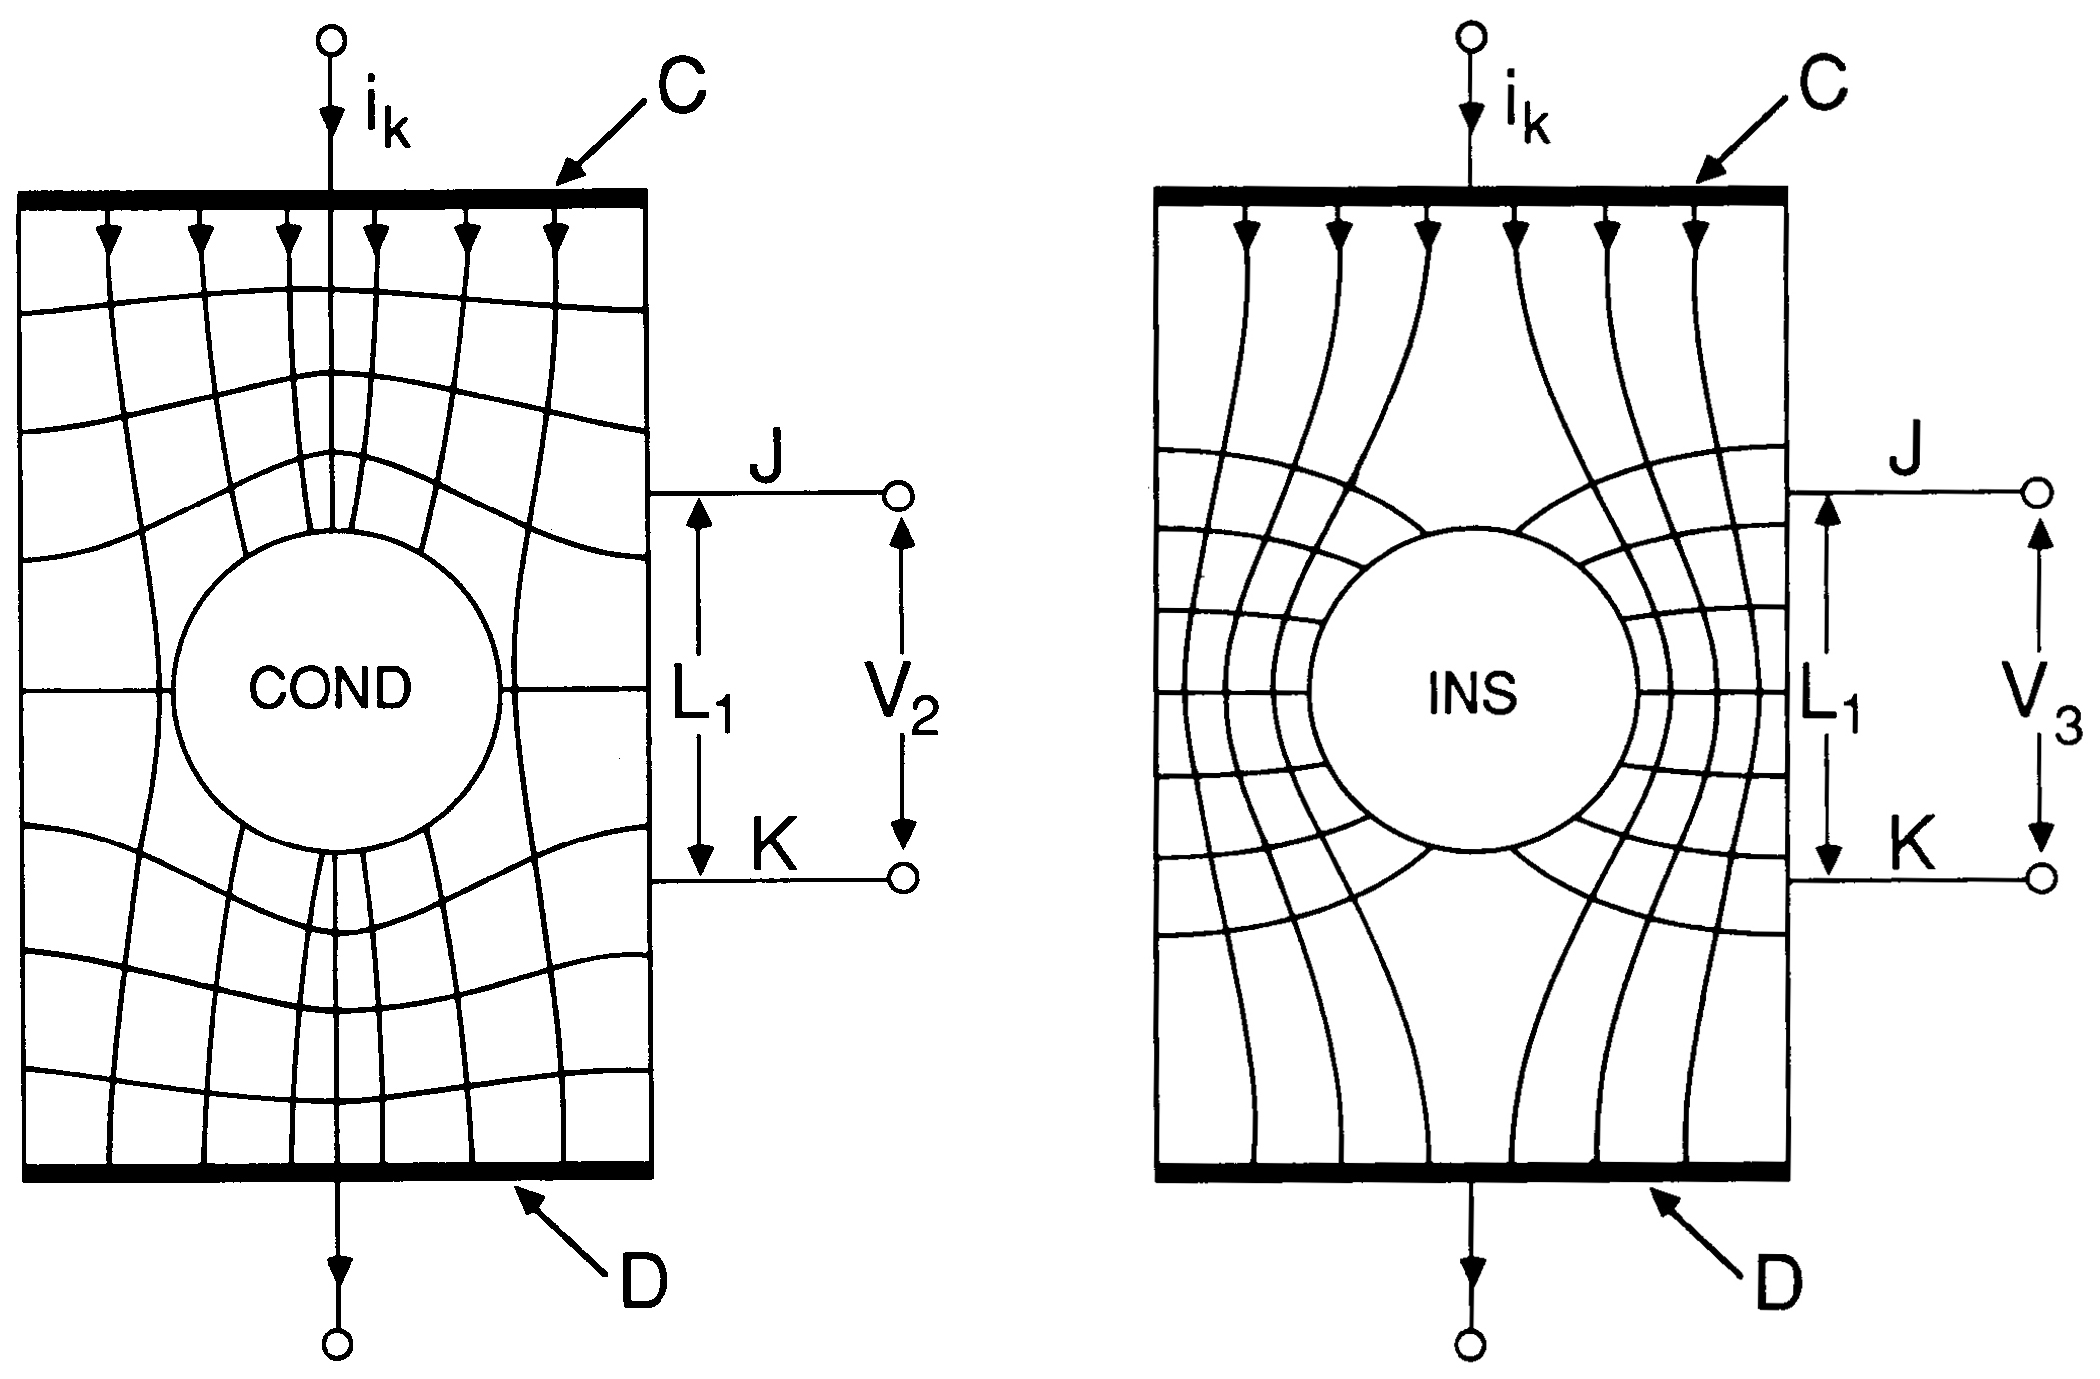
\includegraphics[height=5.6cm]{Background/cond_ins}
	\caption[Distortion of flux lines in the presence of a conductor
	or an insulator]{Distortion of flux lines in the presence of a conductor
	(left) or an insulator (right) when using end-plate electrodes. (Source:
	Baker~\cite{baker1989}. Copyright \textcopyright{} 1989, IEEE.)}
	\label{fig:end_electrodes_distorted}
\end{figure}

\begin{figure}[p]
	\centering
	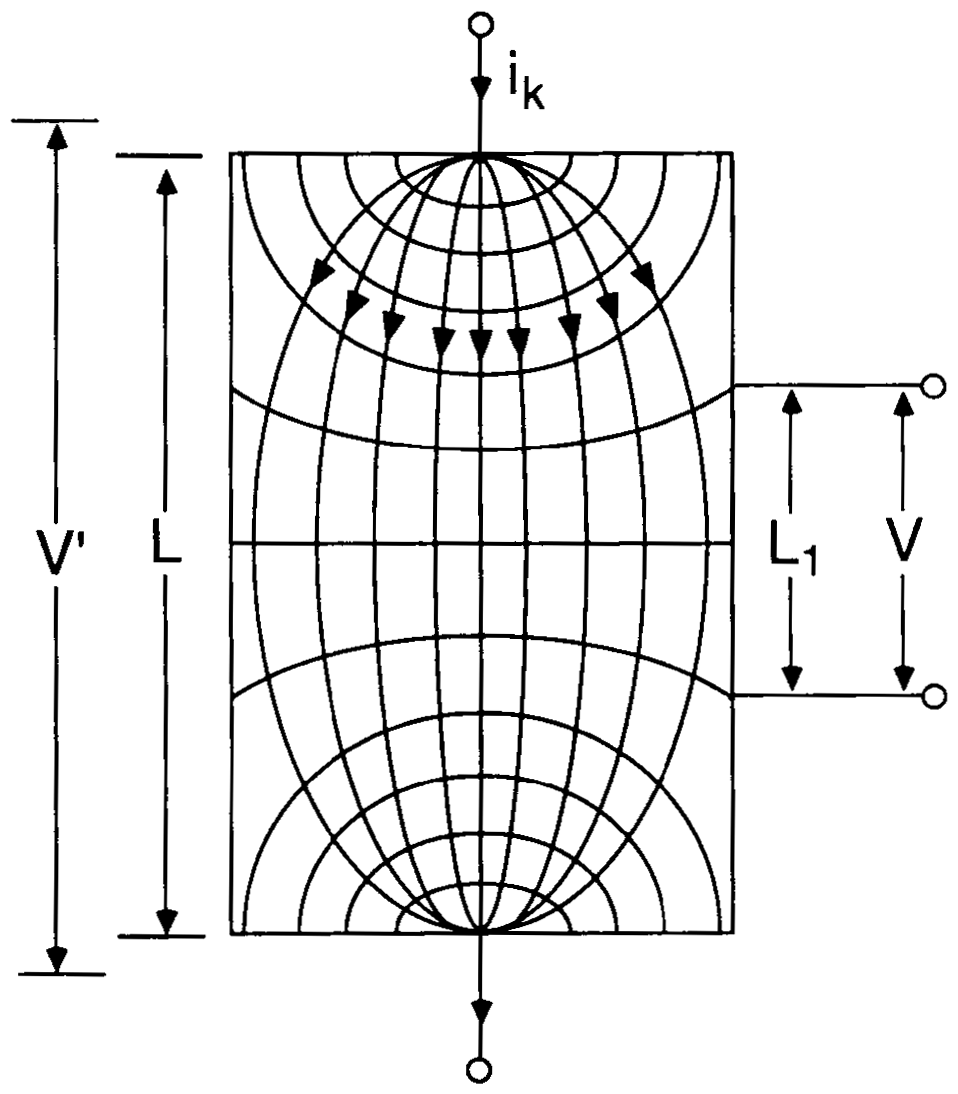
\includegraphics[height=5.6cm]{Background/small_electrodes_flux}
	\caption[Flux lines with small electrodes]{Flux lines with small electrodes.
	Note the non-uniform shape of the current density distribution. (Source:
	Baker~\cite{baker1989}. Copyright \textcopyright{} 1989, IEEE.)}
	\label{fig:small_electrodes_flux}
\end{figure}

Consider again the homogeneous cell, but this time with the end-plate electrodes
replaced by much smaller ones, as per Figure~\ref{fig:small_electrodes_flux}).
Again, the flux lines would deviate from uniformity, but here they would take on
a different pattern, spreading out from the current source through the medium
before reconverging at the sink. Any changes in resistivity that are introduced
in this case would have more impact on the current paths if they are located
near the small electrodes, since this is where the current density is
highest~\cite{baker1989}.

The simulations in this thesis are expected to adhere to the same physics and
thus exhibit both of these patterns. Unlike these simplistic theoretical
examples though, the cochlea consists of many tissues and its three-dimensional
geometry is complex, so the field patterns are not intuitive. Nevertheless, the
current paths will be determined by the anatomical structures as a function of
their material properties, which span a wide range due to large differences in
tissue morphology, and their proximity to the stimulating electrode, which is
small relative to the volume of the cochlea. Note that the cochlear models
themselves are in turn small relative to the entire head, so the reconvergence
of flux lines at the return electrode (as depicted in
Figure~\ref{fig:small_electrodes_flux}) is not expected to occur within the
modelled domain under MP stimulation.

\subsection{Numerical Methods}
\label{sect:numerical_methods}

\subsubsection{Rationale for Computational Modelling}
\label{sect:rationale_for_modelling}

There are several ways these complex electric field patterns could be
characterised in a spatial sense. A rudimentary method would be to measure the
electric potential at numerous points throughout the cochlea of a CI recipient
and then correlate these data with the Cartesian location of each sample to
generate an electroanatomical map~\cite{kral1998}. Such direct measurements
could provide very realistic results since the biological aspects of the system
are inherently accounted for. However, the need to physically intrude into the
cochlear tissues makes this impractical for both \invivo{} and \invitro{}
studies, as noted in \S\ref{sect:knowledge_dev}.

An alternative approach would be to take measurements at fewer, more accessible
locations, and make assumptions about the behaviour of the electric field at
points that are not directly measured~\cite{kral1998}. That is, in essence, the
modelling process, which has become a preferred method of investigation for CI
research. Early efforts used \emph{lumped-element models} (LEMs), which
attempted to represent the electric response of the implanted cochlea as an
equivalent electric circuit. Key locations, such as the position of the
stimulating and measuring electrodes, were connected by a network of electric
circuit components (typically resistors), with each component representing the
response of one or more of the biological tissues along a presumed current
pathway between the connected nodes.

However, a quick comparison of the published LEMs reveals a major flaw in this
approach: since the true shape of the cochlea is ignored, the selection of
electrical elements and connections in these circuits is arbitrary, leading to a
multitude of circuit representations for the same electroanatomical system (see
\S\ref{sect:lumped_element_models}). The models were sufficient insofar as each
LEM was only related back to the corresponding experimental measurements to
yield bulk impedances between two points in that circuit. LEMs are therefore
useful for global insights into CI
stimulation~\cite{machado1996,briaire2000mesh}, but better spatial
representation is required for more generally applicable results.
Indeed, von \bekesy{} noted in his pioneering study that the use of more
elements in the network would provide a closer approximation of the \invivo{}
situation~\cite{vonbekesy1951}.

The development of integrated circuits in the 1970s was a significant milestone
for modelling research because it enabled the development of numerical solution
methods that were computationally intense. Although these numerical methods were
originally developed for structural mechanics, they were later applied to other
types of physics by discretising the appropriate governing equations; in the
case of electromagnetic simulations, these are the aforementioned Maxwell's
equations. Sustained increases in processing power, driven by advances in
microprocessor architectures and manufacturing processes, meant that by the
mid-1980s, a new class of electroanatomical model, based on numerical analysis,
had become viable~\cite{bondeson2005}. These models are generally referred to as
\emph{volume conduction models} (VCMs) because the geometry of the modelled
domain is based on the true three-dimensional (3D) shape of the physical system.
VCMs of the implanted cochlea are reviewed in
\S\ref{sect:volume_conduction_models}.

Numerical methods for bioelectric volume conduction problems have been reviewed
by several
authors~\cite{cendes1989,miller1990,schimpf1998,bondeson2005,johnson2006}. The
main differences between the mathematical formulations of the three most popular
approaches---the \emph{finite difference method} (FDM), the
\emph{finite element method} (FEM), and the \emph{boundary element method}
(BEM)---are summarised below.

\subsubsection{Discretisation and the Finite Difference Method}

All three methods involve approximating the continuous domain with a finite
number of subspaces---a process known as \emph{discretisation} or \emph{mesh
generation}~\cite{reddy1993}. The FDM is the most traditional of the three
approaches and uses the differential form of Maxwell's equations. Under the FDM,
the continuous domain is discretised into a uniform orthogonal grid to yield a
pointwise approximation~\cite{schimpf1998}. At each point, the derivatives are
expressed algebraically as differences between adjacent points in the finite
difference grid. These reference the material properties representing the
electric behaviour of the tissue at that point (namely conductivity and
permittivity). The whole system is then evaluated by recombining the equations
into a global matrix using continuity conditions and solving for the unknown
dependent variable (i.e. the electric potential) at each node using a set of
constraints (namely the \emph{electrical loads} and \emph{boundary
conditions})~\cite{bondeson2005}. The numerical estimate converges to the exact
solution as more subspaces are used; for the FDM, this requires a denser point
cloud.

The FDM is quite simple to implement and compute, making it a good candidate for
time-domain simulations~\cite{bondeson2005}. It is well suited to modelling
devices with man-made geometries and engineering materials, especially those
with straight edges such as cantilever beams. However, geometries that are not
aligned with the grid will suffer from inaccuracies due to the staircase effect
(see Figure~\ref{fig:mesh_comparison}). This means it is unable to accurately
represent the complex organic shapes encountered in anatomical structures, and
faces difficulties imposing certain boundary conditions~\cite{johnson2006}. In
addition, a relatively large number of equations must be solved to achieve a
certain level of accuracy because discretisation using a uniform grid must
account for the finest features of the geometry and the steepest concentrations
in the electric field.

\begin{figure}
    \centering

    \begin{subfigure}[t]{0.5\textwidth}
        \centering
        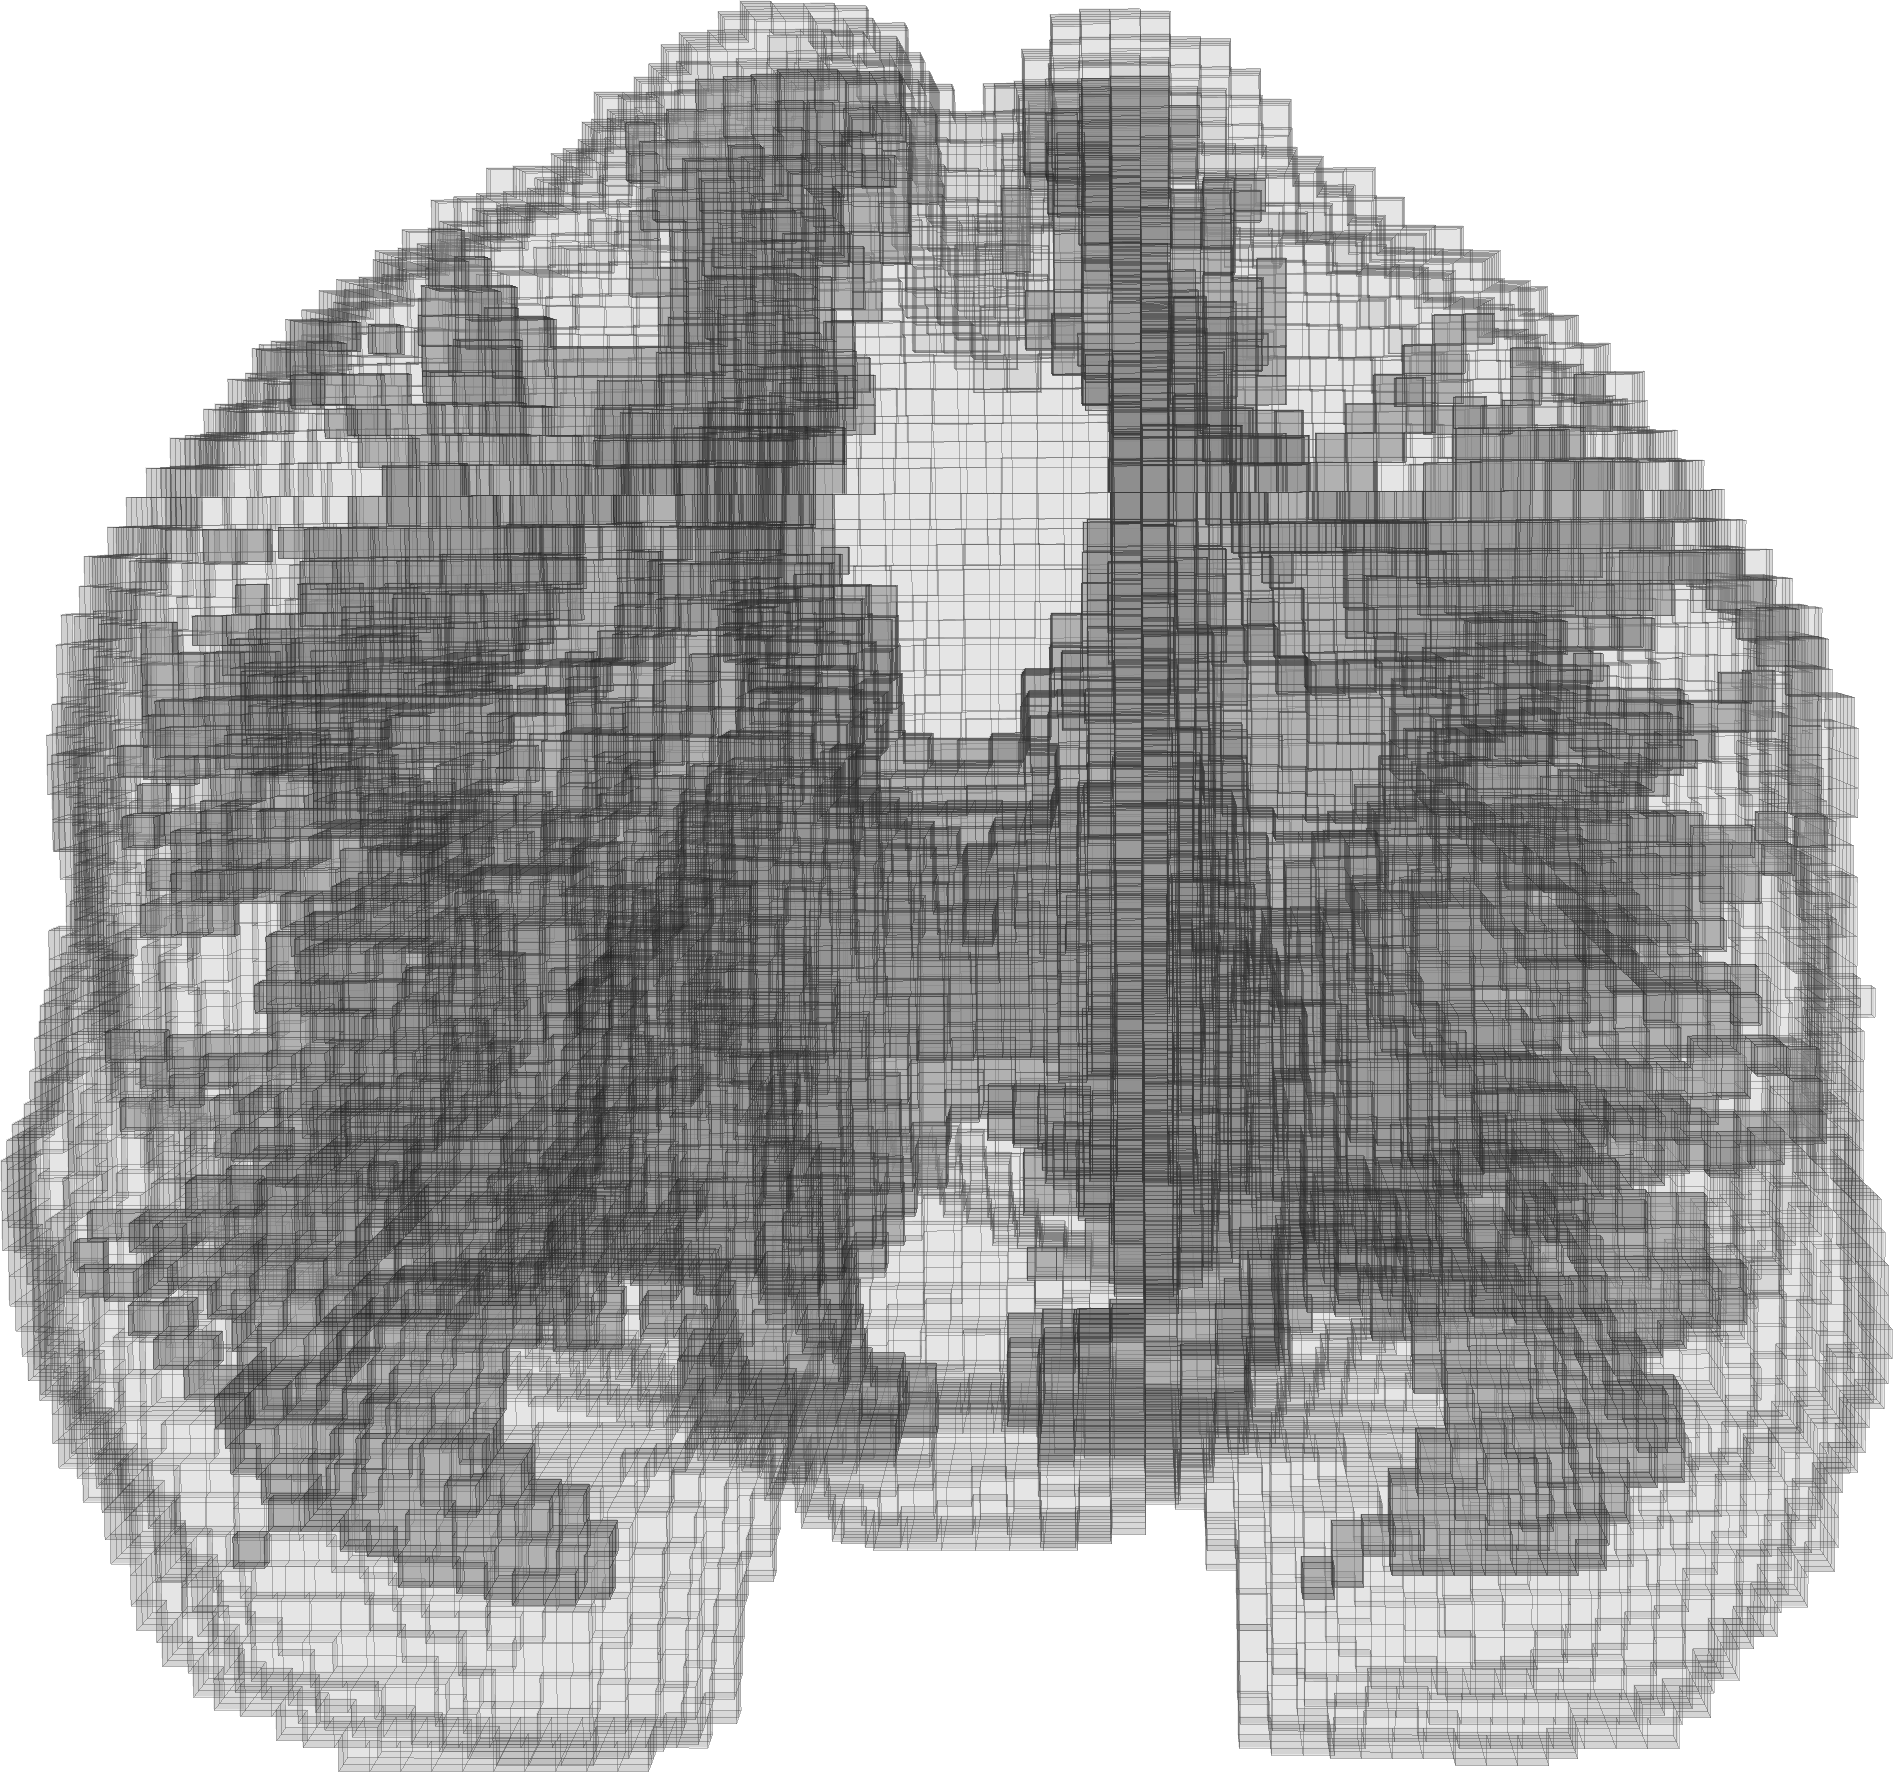
\includegraphics[width=6.5cm]{Background/mesh_grid}
        \caption{ }
        \label{fig:mesh_grid}
    \end{subfigure}%
	\begin{subfigure}[t]{0.5\textwidth}
        \centering
        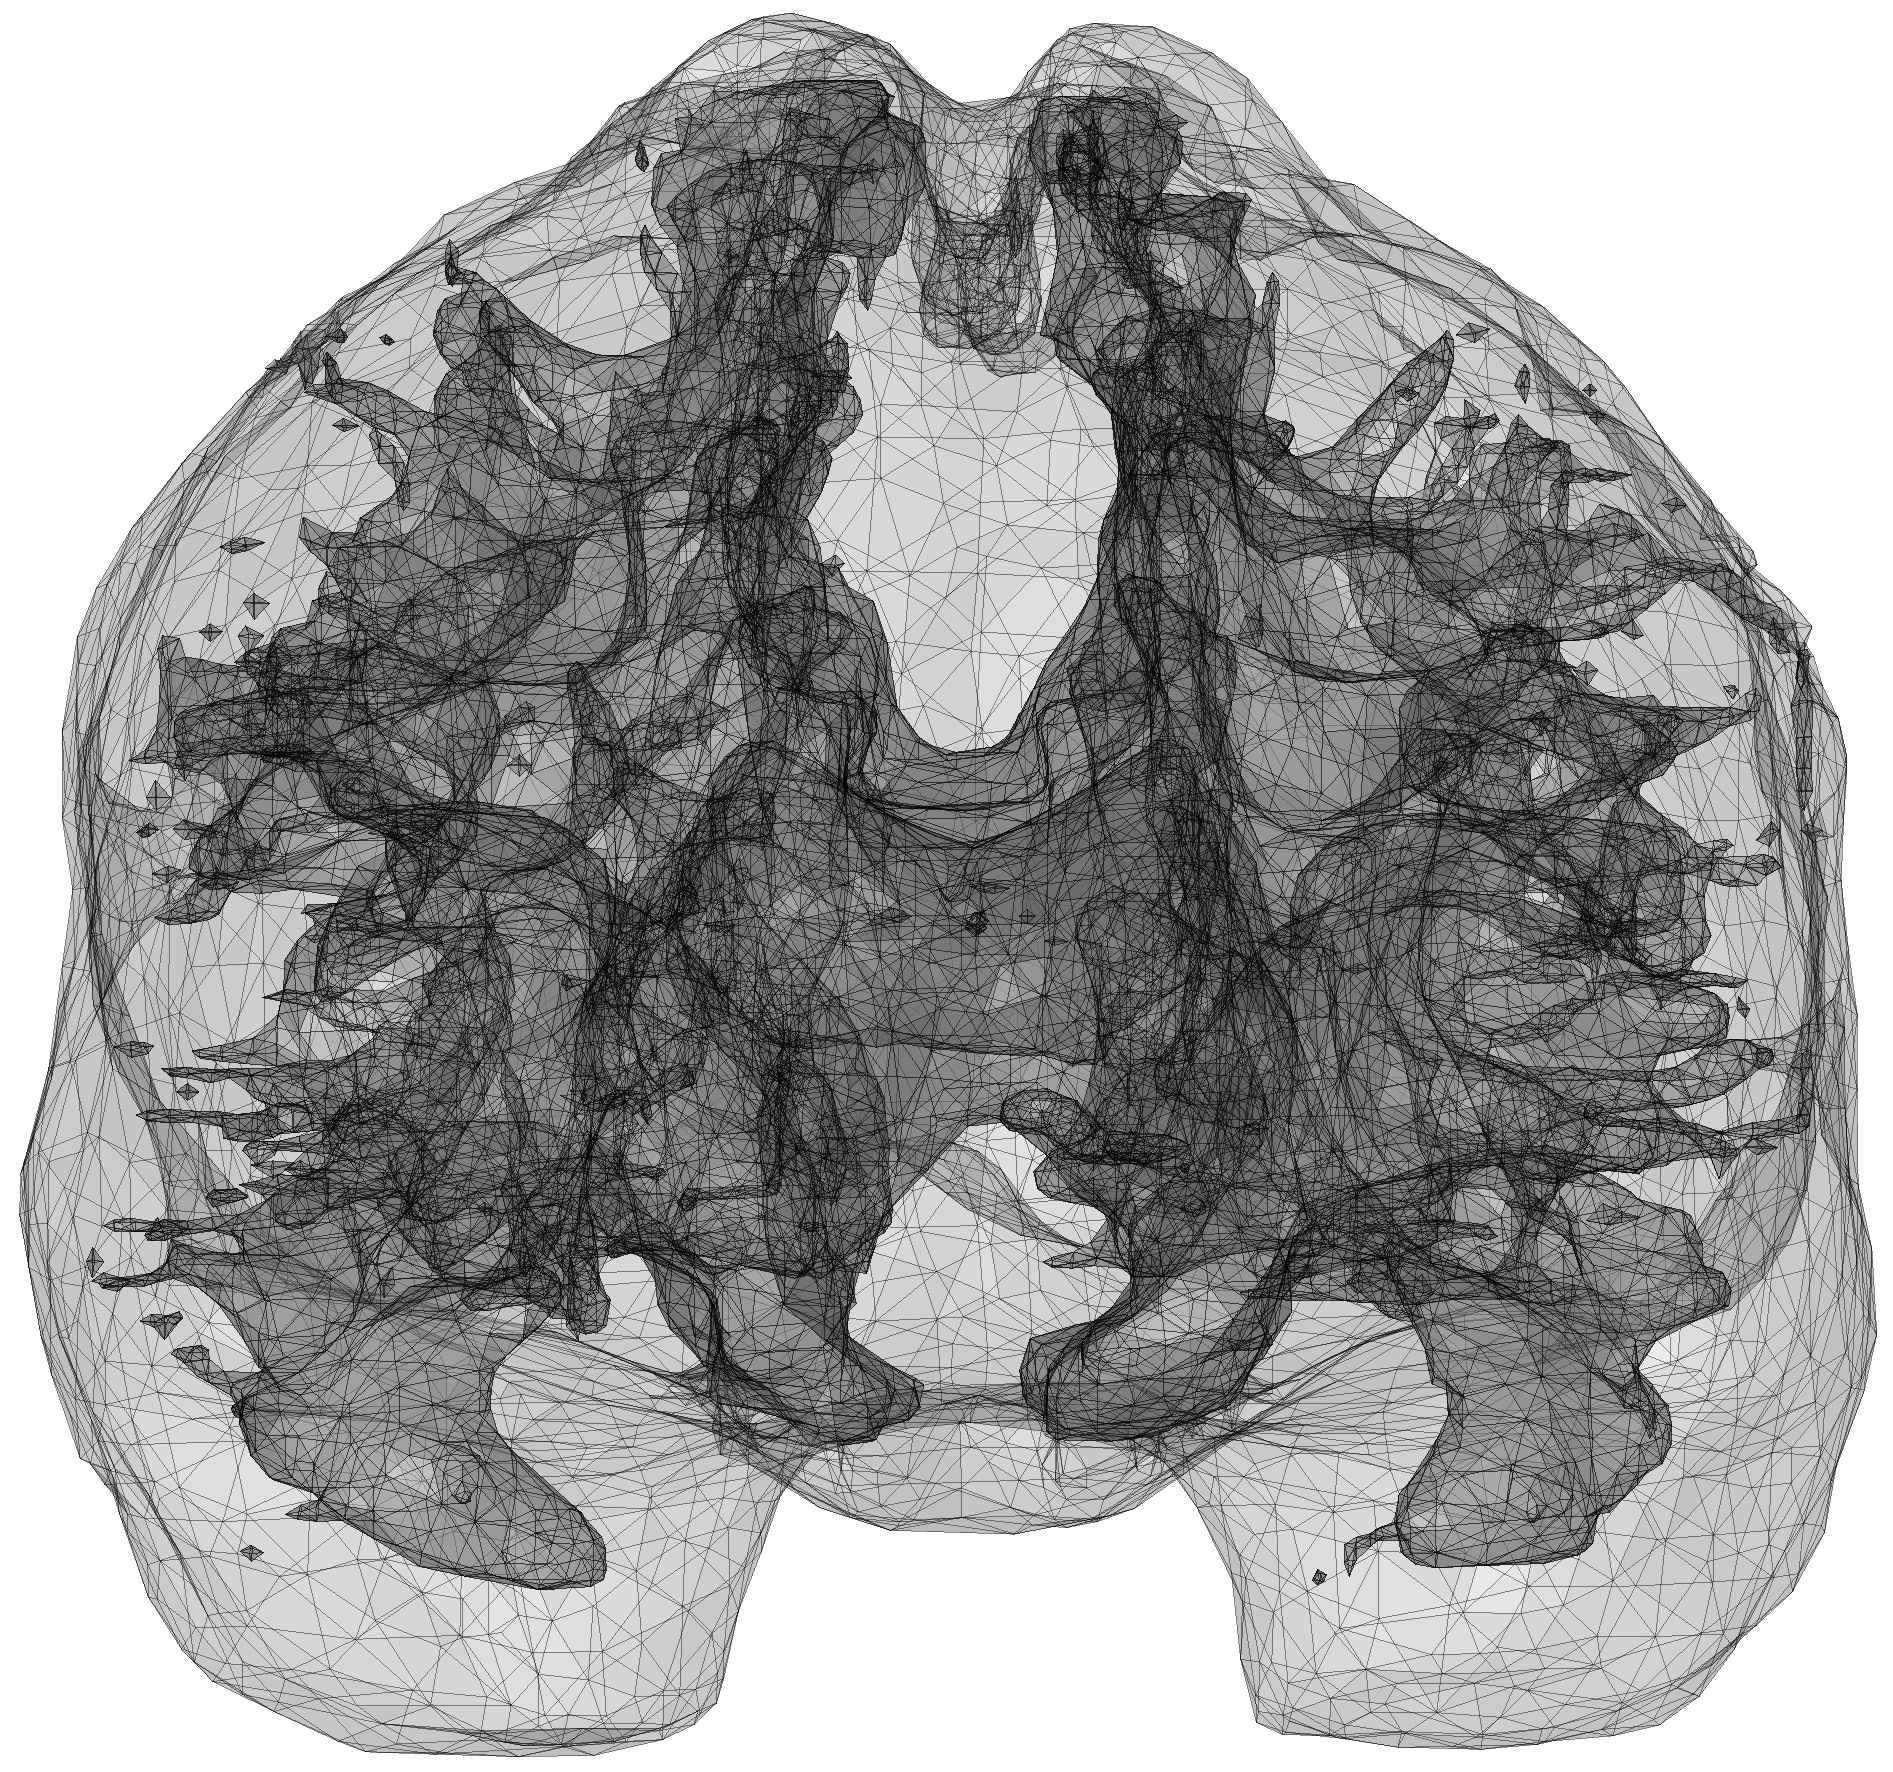
\includegraphics[width=6.5cm]{Background/mesh_free}
        \caption{ }
        \label{fig:mesh_free}
    \end{subfigure}
    
	\caption[Comparison of FDM and FEM meshes]{Comparison of FDM and FEM meshes for
	the brain of HEATHER~\cite{tran2015}. (a) A finite difference mesh exhibits an
	obvious staircase effect. (b) A finite element mesh can produce smoother and
	more realistic boundaries with fewer elements.}
	\label{fig:mesh_comparison}
\end{figure}

\subsubsection{The Finite Element Method}

Generally speaking, the FEM is the most preferred numerical method in
engineering simulations. The main reason for this is its ability to handle
complex geometries~\cite{bondeson2005}. As with the FDM, FEM solvers use
Maxwell's equations in differential form. The difference is that in the FEM, the
continuous domain is discretised into an unstructured mesh.

Instead of using a uniform grid, the points (termed \emph{nodes}) are connected
to form small, discrete regions (\emph{elements}), which have a geometrically
simple (but not necessarily regular nor uniform) shape. Some typical elements
are shown in Figure~\ref{fig:element_types}. In an unstructured mesh, the
distribution of nodes can be non-uniform and non-orthogonal, allowing for a much
smoother representation of curved geometries (cf.
Figure~\ref{fig:mesh_comparison}). This flexible node arrangement also means
that the mesh can be refined locally to improve the accuracy of the solution
around fine geometrical details or regions with steep field gradients without
resorting to a high mesh density throughout the entire domain.

\begin{figure}
	\centering
	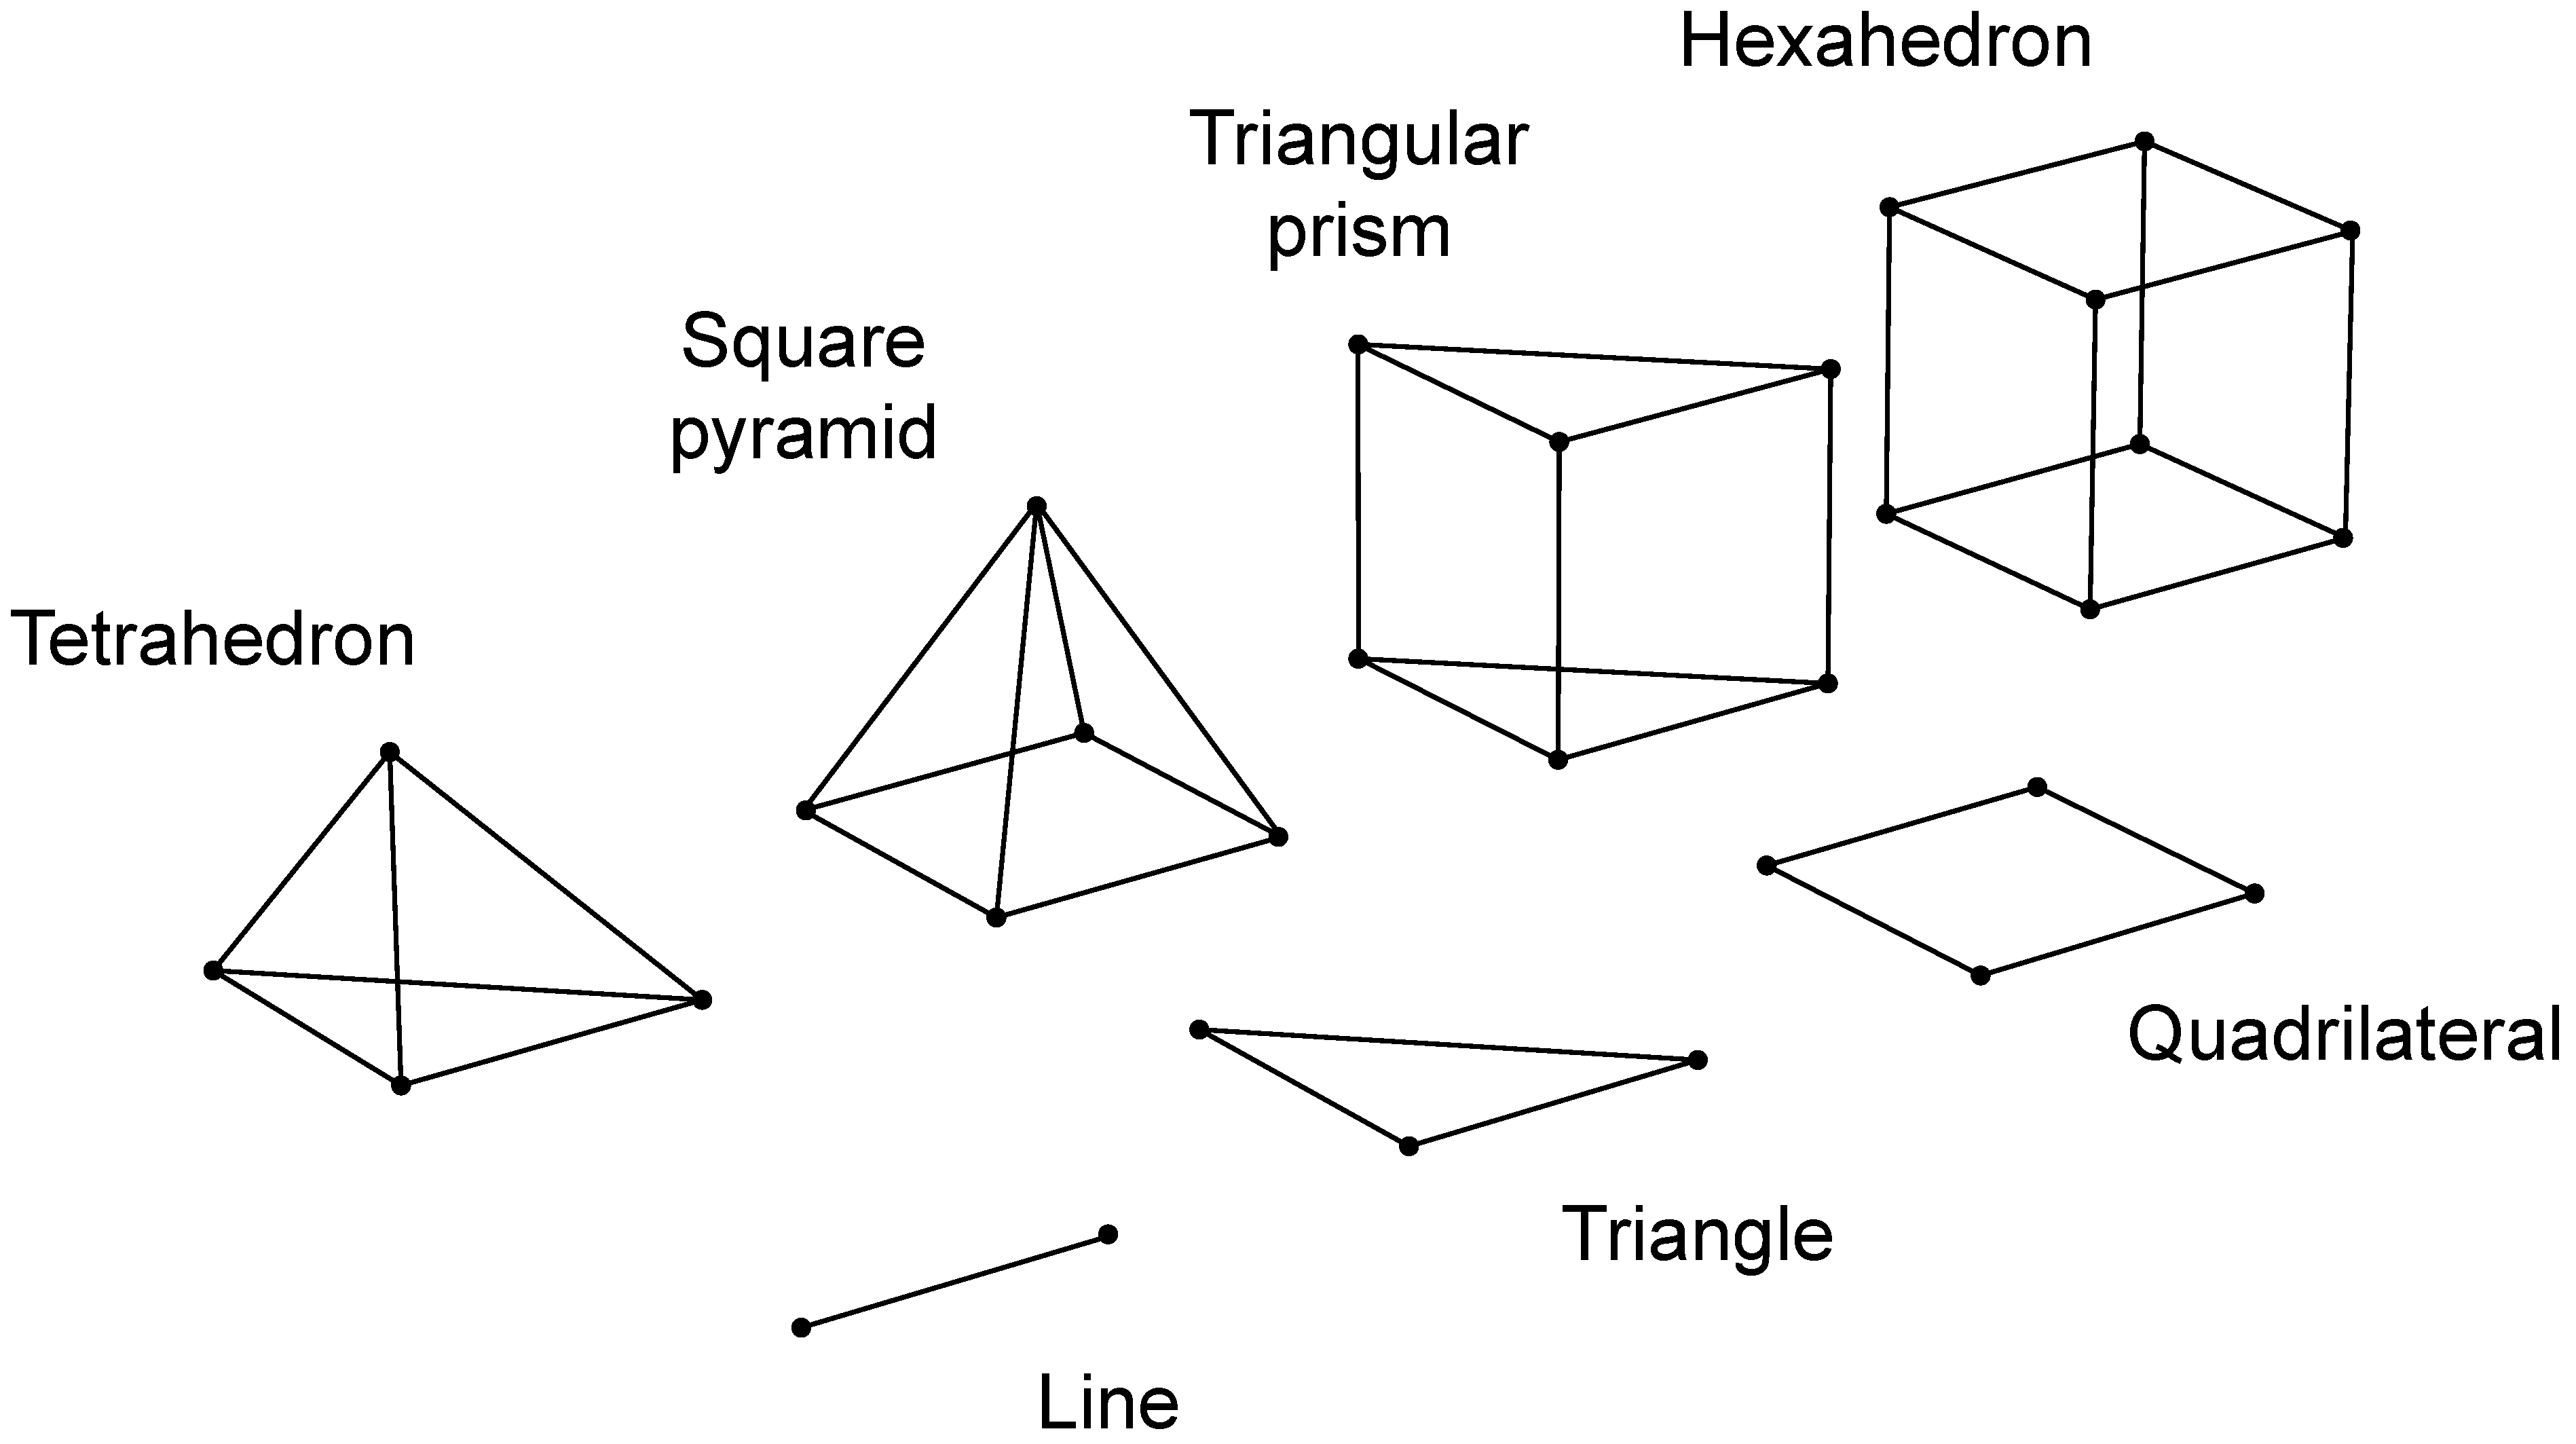
\includegraphics[height=6.2cm]{Background/element_types}
	\caption[Linear finite elements by shape]{Linear finite elements by shape.
	Nodes are shown at each vertex. Quadratically interpolated elements also
	possess mid-side nodes. The final appearance of each element in the mesh is
	typically less regular than those shown here because the elements must conform
	to the geometry of the continuous domain without becoming excessively skewed.
	For 3D problems, the BEM uses planar elements, while the FEM uses volumetric
	elements. (Image adapted from Bondeson~\cite{bondeson2005}. Copyright
	\textcopyright{} 2005, Springer-Verlag.)}
	\label{fig:element_types}
\end{figure}

The formulation of the FEM requires that the change of the dependent variable in
space be defined within each element. This role is fulfilled by an interpolation
function, also known as a \emph{shape function}, which is usually a low order
polynomial defined relative to the values at the nodes of the element. FEM
results can thus also be refined by increasing the order of this shape function.
Because the dependent variable is defined within each element and the global
solution is found by evaluating these with reference to the loads and boundary
conditions, the FEM solution is often described as a piecewise
approximation~\cite{schimpf1998}.

% For all three methods, refinement can be achieved by using smaller subspaces.
% FEM and BEM results can also be refined by using higher order interpolation
% functions, and/or optimising the spatial distribution of the nodes.

\subsubsection{The Boundary Element Method}

The BEM (also known as the \emph{method of moments}) takes a slightly different
approach to the other two methods. In a BEM formulation, the entire volume is
split into compartments by material, and as its name suggests, only the
boundaries between compartments are discretised (using (n--1)-dimensional
elements). However, there are restrictions on the types of geometries that can
be solved. To avoid ambiguity from the dimensional reduction, all compartments
must form closed surfaces and they cannot intersect each other---i.e. they must be
completely nested or completely independent. The material properties assigned to
each compartment must also be constant within the bounding surfaces. These
attributes make the BEM well suited to models that are \emph{homogeneous} (one
material only) and \emph{isotropic} (identical properties in all directions),
for \emph{heterogeneous} models containing only a few materials with similar
properties, and for unbounded problems~\cite{katsikadelis2002}.

Also note that unlike the other two methods, the BEM employs Maxwell's equations
in integral form. The integrand is often decomposed into a singular part, which
has an analytical solution, and a regular part, which is solved numerically.
The analytical component can be an issue for certain classes of problems.

\subsection{Neural Excitation}
\label{sect:neural_excitation}

Calculating the electric field is only one part of the bioelectric problem. For
CI (and other types of electrical) stimulation, it is also of interest to gauge
the consequences of the generated electric field on the excitable tissues, in
this case, the auditory nerves.

\subsubsection{Response of the Neural Membrane}

Like other electrically excitable tissues, the cell membranes of the auditory
nerves contain voltage-gated ion channels (e.g. for \ce{Na^+} influx or \ce{K^+}
efflux) in addition to non-gated channels (e.g. for \ce{Cl^-})~\cite{brown2001}.
The distribution of ion species across the membrane is typically uneven, with
more negative charge inside the cell compared to the outside. This potential
difference, known as the \emph{resting membrane potential}, is on the order of $
-70 $ to $ -90 $ mV, and is maintained by the normal metabolic activity of the
cell. If the ionic permeability of the cell membrane is changed, a local
potential can develop. The cell membrane becomes \emph{depolarised} when the
potential becomes more positive, for example, when there is an influx of
cations; conversely a more negative potential causes it to become
\emph{hyperpolarised}.

Only depolarisation can trigger an action potential~\cite{reilly1998}.
Experiments by Hodgkin and Huxley with unmyelinated squid
axons~\cite{hodgkin1952} and Frankenhaeuser and Huxley with myelinated toad
axons~\cite{frankenhaeuser1964} revealed the ionic mechanisms responsible for
action potential generation. When the electric potential in one region of the
membrane is depolarised to the cell's threshold level, the permeability of the
cell membrane to \ce{Na^+} increases, leading to an influx of \ce{Na^+} which
then further depolarises the cell~\cite{brown2001}. This positive feedback
mechanism quickly reverses the membrane potential in that region, as shown in
Figure~\ref{fig:depolarisation_wavefront}, and the subsequent transfer of charge
from adjacent regions of the membrane causes the depolarisation to propagate. It
is this self-propagating neural impulse that allows signals to be relayed to the
brain. Other voltage-gated channels open after the \ce{Na^+} channels, allowing
\ce{K^+} ions to leave the neuron and restore the resting membrane potential.
The intracellular balance of cations is maintained via sodium-potassium pumps,
which actively transport \ce{Na^+} and \ce{K^+} ions through the membrane
against the concentration gradient.

\begin{figure}
	\centering
	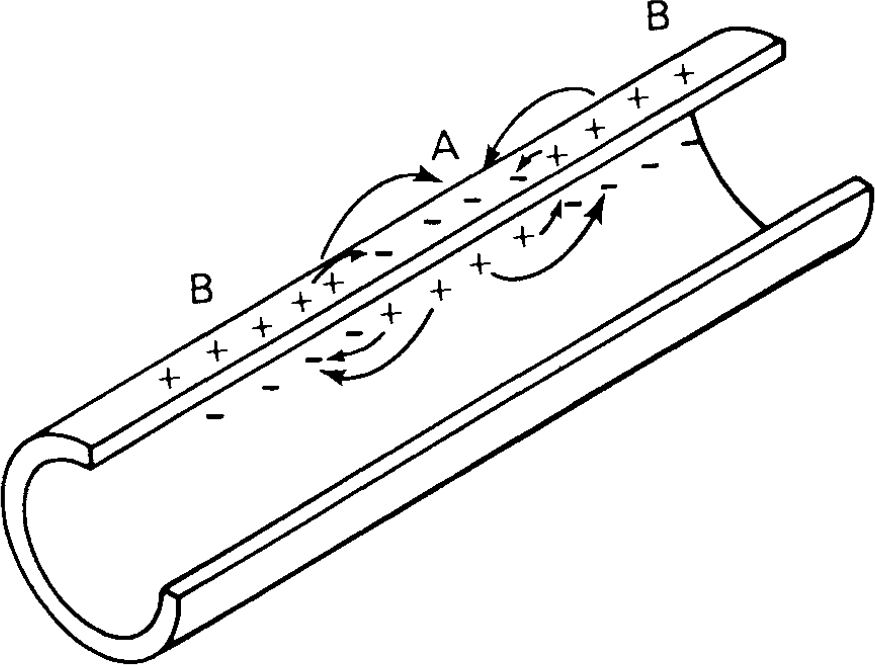
\includegraphics[height=5.2cm]{Background/depolarisation_wavefront}
	\caption[Spread of the depolarisation wavefront]{Spread of the depolarisation
	wavefront. When one region (A) of the neural membrane is depolarised, charge
	stored by the membrane capacitance is transferred from adjacent regions (B),
	thereby propagating depolarisation along the neuron. (Source:
	Reilly~\cite{reilly1998}. Copyright \textcopyright{} 1998, Springer.)}
	\label{fig:depolarisation_wavefront}
\end{figure}

In normal hearing listeners, depolarisation occurs due to the release of
neurotransmitters by stimulated hair cells~\cite{brown2001,martini2006} (recall
\S\ref{sect:normal_hearing}), so the wavefront only propagates in one direction:
away from the hair cell at the peripheral end. For \emph{electrically-evoked}
neural stimulation, the active electrodes set up an artificial electric
field, causing voltage disturbances along the membrane which drive ions across
the channels in the membrane~\cite{reilly1998}. The location of the stimulating
electrodes typically induces depolarisation somewhere in the middle of the
neuron, creating a bidirectional depolarisation wavefront
(Figure~\ref{fig:depolarisation_wavefront}).

Myelination of nerve fibres is a biological adaptation that permits faster
conduction velocities while retaining small fibre diameters~\cite{brown2001}.
Glial cells form a non-conductive \emph{myelin sheath} around the axon, with
small gaps between adjacent sheaths known as \emph{nodes of Ranvier}. The
structure means that ionic current can only cross the membrane at the nodes, so
the wavefront jumps along the axon from one node to the next instead of simply
to adjacent regions of the neural membrane. This process is known as
\emph{saltatory conduction}.

\subsubsection{Theoretical Models}

Several approaches are available for explaining the membrane behaviour. Early
models analysed current traversing a localised patch of neuronal membrane.
However, Reilly found that ``the force driving current into the membrane is the
external field distribution \emph{along the axon}, which cannot be described by
the current density at a single point''~\cite{reilly1998}. This suggests that
the spatial and temporal interactions along the entire length of the neuron must
be considered to properly represent action potential generation and
propagation~\cite{strelioff1973,rattay1990,reilly1998,astrom2014}. On the other
hand, a recent study of deep brain stimulation modelling found that activation
can be approximated without coupling the finite element solution to an axon
model~\cite{astrom2014}. Nonetheless, axon models are more likely to account for
spatial phenomena, such as the prevention of action potential propagation by a
sufficiently large ``anodal surround''~\cite{ranck1975}.

Many quantitative models of neural excitation have consequently been developed
based on cable theory, with the neuron being modelled as a long one-dimensional
cable as illustrated in Figure~\ref{fig:membrane_circuit}. McNeal's myelinated
nerve model~\cite{mcneal1976} was the first to consider stimulation due to
finite duration current pulses from extracellular electrodes. Here, the nodes of
Ranvier were spaced at regular intervals, and the myelin sheath was assumed to
be a perfect insulator. Only the central excitation node was modelled with
non-linear membrane conductances, so the model was applied to subthreshold
stimulation. Despite these simplifications, the McNeal model could account for a
variety of electrophysiological observations.

\begin{figure}
	\centering
	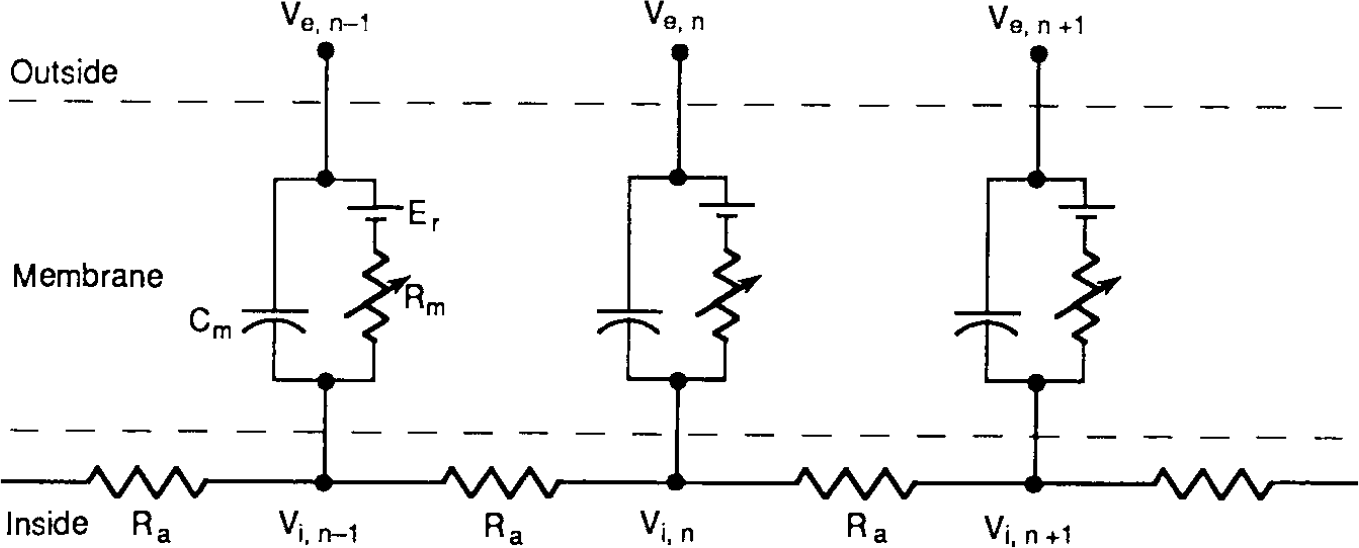
\includegraphics[height=5.1cm]{Background/mcneal_circuit}
	\caption[Equivalent circuit model for excitable membranes]{Equivalent circuit
	model for excitable membranes. (Source: Reilly~\cite{reilly1998}. Copyright
	\textcopyright{} 1998, Springer.)}
	\label{fig:membrane_circuit}
\end{figure}

Under this model, the membrane potential is described by:
\begin{equation}
	\frac{dV_n}{dt} = \frac{1}{C_m}[G_a(V_{n-1}-2V_n+V_{n+1}
	+V_{e,n-1}-2V_{e,n}+V_{e,n+1}) - I_{i,n}] \hspace{1em} (n \neq 0)
	\label{eqn:mcneal_membrane_potential}
\end{equation}
where $ V_n = V_{i,n} - V_{e,n} $ is the potential difference across the
membrane at the $ n $th node along the fibre (with a positive value indicating
depolarisation), $ t $ is time, $ C_m $ is the membrane capacitance of the node,
$ G_a = \nicefrac{1}{R_a} $ is the internodal conductance, $ V_{e,n} $ is the
external nodal voltage, and $ I_{i,n} $ is the internal ionic current flowing in
the node. The ionic current term can be modelled linearly using Ohm's law for
subthreshold stimulation, or non-linearly when at or near the excited state
using differential equations, such as those of Frankenhaeuser and
Huxley~\cite{frankenhaeuser1964}, or stochastic methods~\cite{bruce1999}.

In his review paper on empirical studies of electrical stimulation, Ranck found
that depolarisation was primarily caused by the extracellular voltage becoming
more negative (i.e. intracellular potential changes were
small)~\cite{ranck1975}. He also found that current flow along the long axis of
the neuron is more likely to depolarise it than transverse current. These
findings were strongly supported by McNeal's theoretical model. Subsequent
studies extended McNeal's basic framework. Reilly's spatially extended
non-linear node (SENN) model, for instance, implemented several non-linear
nodes~\cite{reilly1985} and gave further weight to the accepted tenet that
stimulation occurs where neurons end or bend, or where the spatial gradient of
the electric field is highest~\cite{reilly1998}. Colombo and Parkins modified
the McNeal neuron geometry to match measurements by Liberman and Oliver in the
cat~\cite{liberman1984}, and implemented additional non-linear
nodes~\cite{colombo1987}. Rattay made the framework more robust, accounting for
both subthreshold and superthreshold stimulation as well as both myelinated and
unmyelinated fibres~\cite{rattay1986}. He found that for electrical stimulation,
``the second derivative of the external potential in the direction of the axon
is responsible for all the activations inside the axon''~\cite{rattay1986}.
Since it was a necessary condition for neural excitation, Rattay called this the
\emph{activating function} (AF). The AF can be expressed for both unmyelinated
and myelinated neurons respectively as:
\begin{equation}
	\text{AF} = \frac{\partial {^2} V_e}{\partial x^2} \approx
	\frac{V_{e,n-1}-2V_{e,n}+V_{e,n+1}}{\Delta x^2}
	\label{eqn:af}
\end{equation}
where $ x $ is displacement along the nerve fibre. Further refinements to the
model were later added to make the model more applicable to human cochlear
neurons~\cite{rattay1999,rattay2001neuron}.

Another prominent excitation model in CI research is the generalised Schwarz,
Eikhof, and Frijns (GSEF) model developed by Frijns \etal~\cite{frijns1995},
intended for use in models of the guinea pig cochlea. This model was based on
earlier work by Schwarz and Eikhof with myelinated rat fibres~\cite{schwarz1987}
and Frijns and ten Kate's modifications of the SENN model~\cite{frijns1994}.
Like Colombo and Parkins, it was based on mammalian neural kinetics, with
non-uniform internodal lengths in accordance with the morphological data of
Liberman and Oliver~\cite{liberman1984}. Each nerve fibre included 16 non-linear
nodes. The assumption of perfectly insulating myelin sheaths was retained.

The main weakness in the majority of these models is that they mix empirical
results from different animal species. This does not necessarily invalidate the
model, since neural kinetics can be similar across species and the models are
tuned to fit experimental data, but there is still an abstraction gap between
these theoretical models and \insitu{} nerve fibres. This was particularly
evident in Whiten's modelling work~\cite{whiten2007} (see
\S\ref{sect:whiten})---despite having a patient-specific model with ideal
archival data for comparison, he found that the model was weakest when compared
against the psychophysical data. Other aspects of the modelling methodology may
have played a part in this discrepancy, suggesting that significant care and
attention to detail need to be exercised throughout the reconstruction process.

More recent developments in the area of neuronal modelling have been published
by a group in Melbourne, Australia. In a series of four
papers~\cite{meffin2012,tahayori2012,meffin2014,tahayori2014}, Meffin~\etal{}
developed a more robust model of extracellular stimulation that goes beyond the
cable theory models by incorporating the cellular composition of the neural
tissue, including the effect of the confined extracellular space, as well as
both longitudinal and transverse modes of stimulation. The formulation
calls for parallel unmyelinated neurons, which may be applicable to the
spiral ganglion, but has yet to be implemented in a VCM of the cochlea.

\section{Electric Models of the Cochlea}

Existing electric models of the cochlea fall into two categories: lumped-element
models and volume conduction models. Prominent examples are described in the
following sections, grouped by primary author and sorted in chronological order
of appearance.

% ========================================================================= LEMs

\subsection{Lumped-Element Models}
\label{sect:lumped_element_models}

\subsubsection{Von \bekesy{} (1951)}

Von \bekesy's LEM~\cite{vonbekesy1951} was the pioneering effort to understand
the electroanatomy of the cochlea. In his experimental work with explanted
guinea pig cochleae, von \bekesy{} found that the otic capsule was a good
insulator and mused that the grounding resistance must therefore lie in the
modiolus. Additional measurements indicated that ``the main grounding pathway of
the cochlea is through the acoustic nerve to the brain''~\cite{vonbekesy1951},
and that there would be substantial cross-conduction between the turns of the
cochlea because the nerves and blood vessels of the modiolus enter the cochlear
partition along the entire length of the spiral. These observations gave birth
to the idea that grounding the auditory nerve is a good choice for representing
the cochlea's electrical behaviour.

In light of these findings, von \bekesy{} sought to explain the attenuation
of voltage along the cochlear partition by considering two extreme cases:
(i)~the cochlear partition is a very \emph{poor} insulator, so the intracochlear
spaces would resemble a homogeneous conducting body (like a drop of fluid); and
(ii)~the cochlear partition is a very \emph{good} insulator, so the cochlea was
effectively a fluid-filled tube separated into two conjoined canals (analogous
to a \emph{transmission line}). He found that while neither extreme was
realistic for the entirety of the cochlea, the former was more suitable at the
helicotrema and the latter near the round window.

Focusing on the basal turn, he created the transmission line model in
Figure~\ref{fig:model_vonbekesy}. The model consisted of a 3D network of
resistive elements, representing current paths along the scala vestibuli, the
scala tympani, and the cochlear partition, the grounding pathway through the
nerves and blood vessels in the modiolus, and additional resistances to account
for cross-turn effects.

\begin{figure}
	\centering
	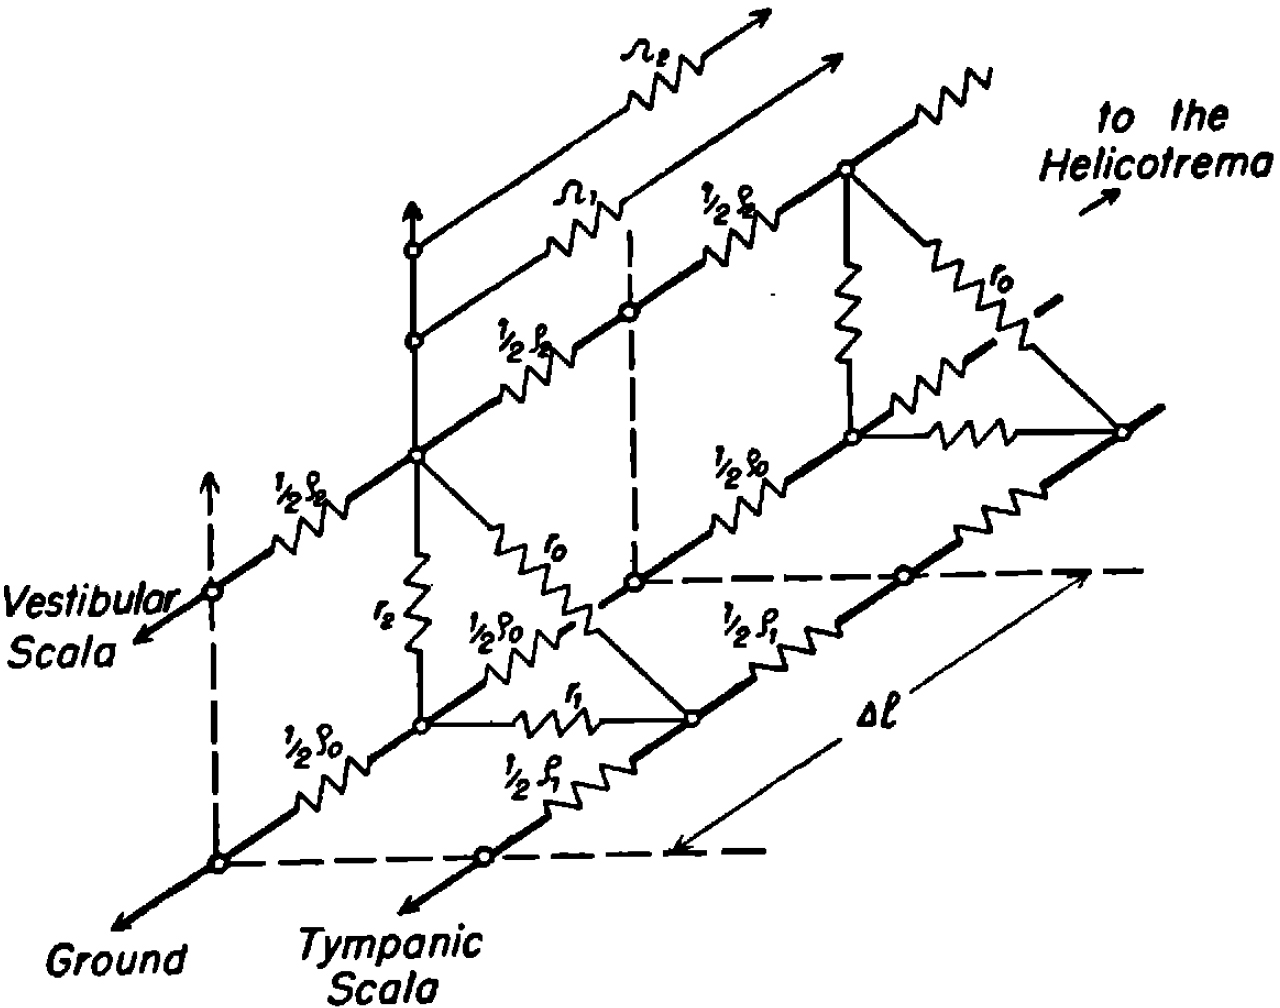
\includegraphics[height=6.8cm]{Background/vonbekesy_fig11a}
	\caption[The von \bekesy{} model]{The von \bekesy{} transmission line model,
	representing a small section of the cochlear tube near the basal end. (Source:
	von \bekesy~\cite{vonbekesy1951}. Copyright \textcopyright{} 1951,
	Acoustical Society of America.)}
	\label{fig:model_vonbekesy}
\end{figure}

The von \bekesy{} model was a good start to electroanatomical modelling of the
cochlea, but it had several shortcomings. The model accounted for many of the
possible current paths, but it failed to consider others like the scala media,
the cerebrospinal fluid (CSF), and the spiral ligament. Detail was also lost
where different tissue types were combined into single elements; for instance,
the organ of Corti and the basilar membrane were modelled together as the
cochlear partition, and the nervous and vascular pathways in the modiolus were
combined into a single grounding resistance. It is impossible to determine which
tissue path is preferred in these lumped regions. Von \bekesy{} also found that
capacitive effects were not important. However, the 1000 Hz stimulus signal used
in these impedance measurements is well below the 10 kHz threshold typically
required for such effects to manifest~\cite{geddes1967}.

\subsubsection{Johnstone \etal{} (1966)}

Johnstone~\etal{} were also interested in discovering more about the electrical
pathways of the guinea pig cochlea, particularly the resistances of the three
boundary walls of the scala media. They proposed a relatively simple LEM
(Figure~\ref{fig:model_johnstone}) that aimed to synthesise the measurements of
both von \bekesy{} and Misrahy~\cite{misrahy1958} into one consistent
model~\cite{johnstone1966}.

\begin{figure}
	\centering
	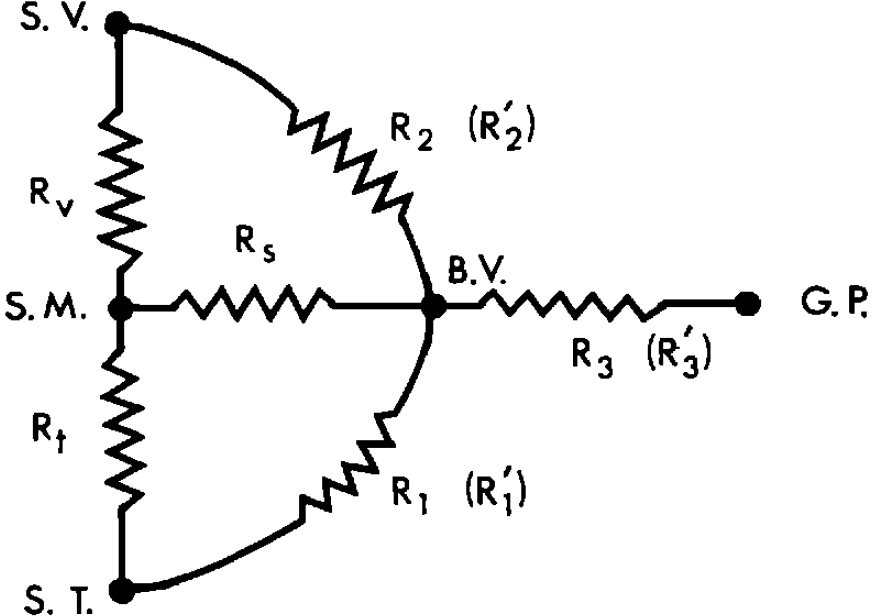
\includegraphics[height=4.8cm]{Background/johnstone}
	\caption[The Johnstone model]{The Johnstone model. SV=scala vestibuli; SM=scala
	media; ST=scala tympani; BV=blood vessels; GP=guinea pig (body). (Source:
	Johnstone~\etal~\cite{johnstone1966}. Copyright \textcopyright{} 1966,
	Acoustical Society of America.)}
	\label{fig:model_johnstone}
\end{figure}

The Johnstone model differs from the von \bekesy{} model in several respects. It
was devised as a 2D representation of the experimental setup through one turn of
the cochlea, and does not directly account for longitudinal current flow or
cross-turn effects. As per the focus of this study, the main pathways considered
were the boundaries of the scala media, i.e. Reissner's membrane, the organ of
Corti and associated structures on the basilar membrane, and the spiral ligament
via the stria vascularis. There is a strong emphasis on the role of the cochlear
blood vessels as a conductive pathway that links the scalae. Like von \bekesy,
Johnstone~\etal{} also suggested that the grounding resistance would be through
the structures of the internal auditory meatus, in conjunction with the cochlear
artery. The experimental technique used also differed, with the injection of
square current pulses akin to those used in contemporary CI systems, though with
a significantly longer pulse width.

Overall, the Johnstone model added some extra detail around the scala media
while ignoring detail from other regions of the cochlea. It still favoured a
purely resistive formulation. Johnstone~\etal{} admitted that the model was
``the simplest measurable network'', even
``oversimplified''~\cite{johnstone1966}, but was nonetheless able to reconcile
the results of earlier studies and provide reasonable voltage predictions.

\subsubsection{Strelioff (1973)}

Another LEM was proposed by Strelioff in 1973~\cite{strelioff1973} (see
Figure~\ref{fig:model_strelioff}). It aimed to study the spatial distribution of
electric potentials and currents in the guinea pig cochlea arising from acoustic
stimulation.

\begin{figure}
	\centering
	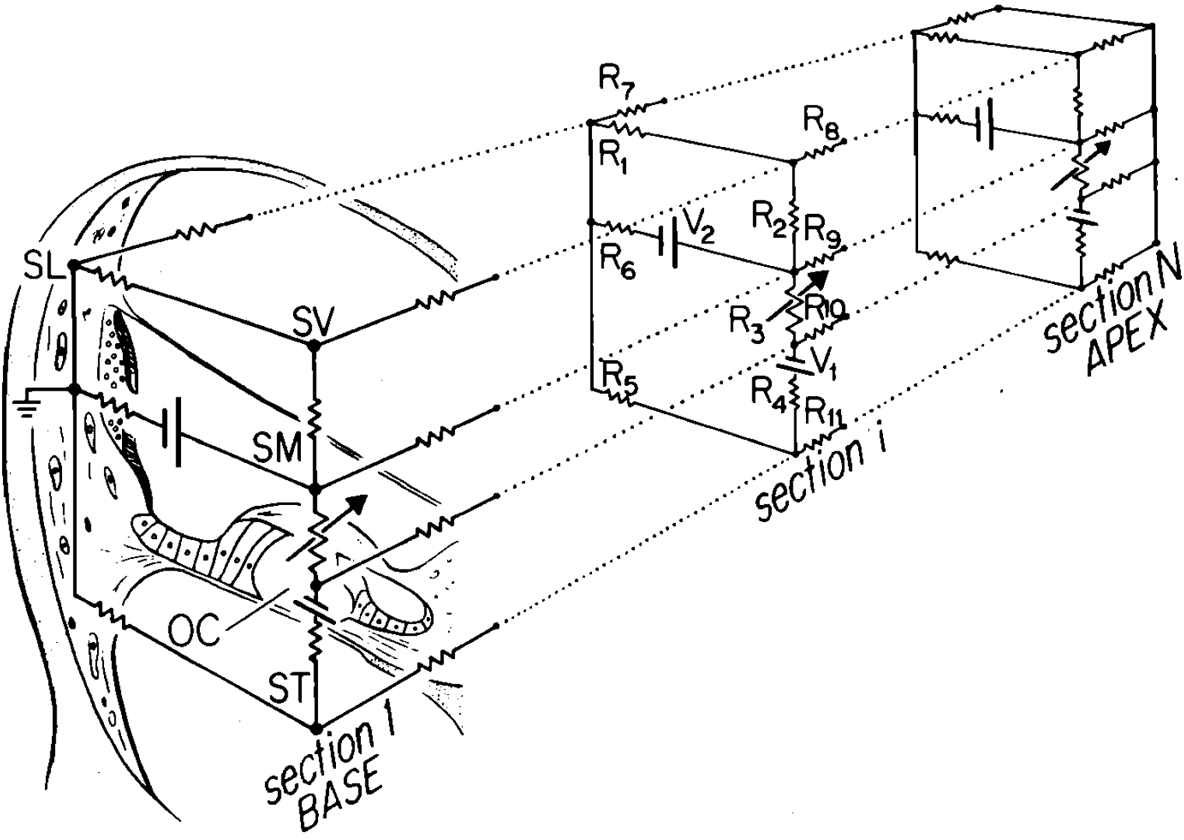
\includegraphics[height=6.5cm]{Background/strelioff}
	\caption[The Strelioff model]{The Strelioff model. SL=spiral ligament; SV=scala
	vestibuli; SM=scala media; OC=organ of Corti; ST=scala tympani. (Source:
	Strelioff~\cite{strelioff1973}. Copyright \textcopyright{} 1973,
	Acoustical Society of America.)}
	\label{fig:model_strelioff}
\end{figure}

In terms of the layout of the circuit elements, the Strelioff model was arguably
more accurate than either the von \bekesy{} or Johnstone models. It returned to
a linear 3D network similar to von \bekesy's model, with a series of over 90
cross-sectional circuits connected via longitudinal resistances. Each
cross-section included nodes in five different fluid-filled spaces (the scala
vestibuli, scala media, and scala tympani, the tunnel of Corti, and the spiral
ligament), resistances to represent the pathways between adjacent nodes, and
battery elements to represent endocochlear potentials.

Weaknesses of the Strelioff model include the decision to use a linear model to
represent the entire length of cochlear spiral, which ignores cross-turn effects
from the true 3D geometry. Lumping the longitudinal pathways along the modiolus
with those of the spiral ligament and ground is also questionable given that
they lie on opposite sides of the scalae. The cochlear vasculature is not
explicitly accounted for in the model, and no capacitive effects were
incorporated despite an admission that they undoubtedly exist. Strelioff also
noted that the use of discrete elements could reduce accuracy, but estimated
that the results were accurate to within 5\% of a continous model based on an
extrapolation of some preliminary results.

\subsubsection{Black and Clark (1980)}

The Black and Clark model~\cite{black1980,black1983}, shown in
Figure~\ref{fig:model_black}, was the first effort to investigate the behaviour
of the cochlea during electrical stimulation for hearing restoration. The
geometry of the model was based on that of Johnstone \etal, but extended to 16
cross-sections in the transverse direction as per the transmission line models.
Resistance values were fitted to the range of published experimental
measurements via scaling.

\begin{figure}
	\centering
	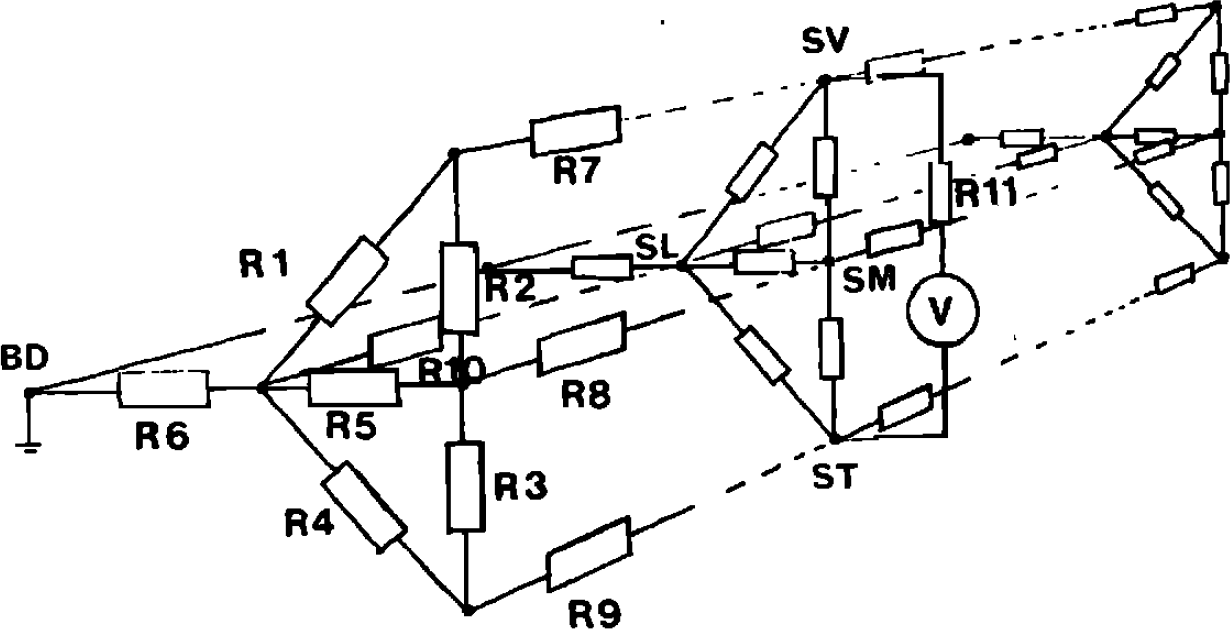
\includegraphics[width=9cm]{Background/black_clark}
	\caption[The Black and Clark model]{The Black and Clark model. SV=scala
	vestibuli; SM=scala media; ST=scala tympani; SL=spiral ligament; BD=animal
	body. (Source: Black and Clark~\cite{black1980}. Copyright \textcopyright{}
	1980, Acoustical Society of America.)}
	\label{fig:model_black}
\end{figure}

In conjunction with some additional measurements, the model revealed differences
in stimulation specificity between various electrode configurations; in
particular, that BP stimulation resulted in the highest specificity of the
tested configurations. They also noted that the spread of current through the
neural tissues may be different from the spread of potentials through the
scalae, so voltage traces on their own were insufficient for inferring the
effect on neural excitation.

Since they use the same circuit layout for the cross-sectional slices, this
model shares some of the weaknesses of the Johnstone model. An additional
concern of this study lies in the continual rescaling of model parameters to
force-fit the experimental data. The authors acknowledged in the discussion that
the model was too simple for some applications, such as modelling length
constants under BP stimulation.

\subsubsection{Suesserman and Spelman (1993) \& Machado and Toumazou (1995)}

In their studies of the cochlea, Suesserman and Spelman realised that the
physical presence of the electrode array and the deterioration of cochlear
structures with the onset of deafness both had an effect on the current paths,
which had not been accounted for in the modelling literature. As such, they
created an extension of the Strelioff model to better match the \invivo{}
electrical behaviour during electrical stimulation~\cite{suesserman1993}.

Their model represented the first turn of the cochlea using 51 cross-sectional
slices with a thickness of 200 $ \upmu $m, as illustrated in
Figure~\ref{fig:model_suesserman}. It added a new node for the stimulating
electrode in the scala tympani and new elements to capture the membrane
capacitances ignored in previous studies. The battery elements representing
endocochlear potentials were removed since the focus was on exogenous
stimulation. The model parameters were adjusted to account for the increase in
resistance along the scala due to the presence of the electrode array and
matched to Spelman's earlier experimental work on implanted guinea pig
cochleae~\cite{spelman1982}.

\begin{figure}
	\centering
	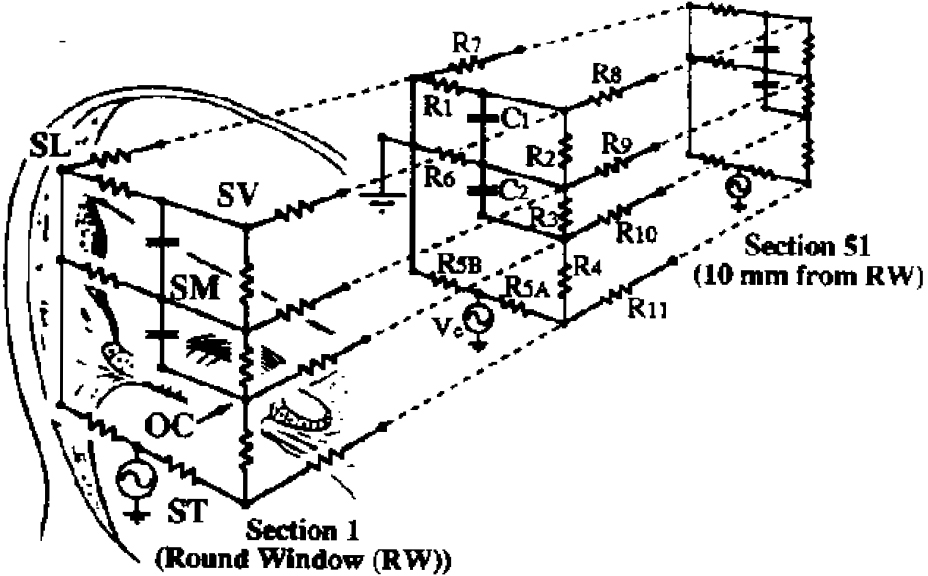
\includegraphics[height=6cm]{Background/suesserman}
	\caption[The Suesserman and Spelman model]{The Suesserman and Spelman
	model. SL=spiral ligament; SV=scala vestibuli; SM=scala media; OC=organ of
	Corti; ST=scala tympani. (Source: Suesserman and
	Spelman~\cite{suesserman1993}. Copyright \textcopyright{} 1993, IEEE.)}
	\label{fig:model_suesserman}
\end{figure}

The Suesserman and Spelman model was the most accurate LEM of the implanted
cochlea. However, like prior studies, it assumed that the cochlea could be
uncoiled. With the emphasis firmly on the modelling of electrical stimulation,
it is important to consider that the neural structures closer to the modiolus
were still not included since the uncoiling assumption becomes less applicable
in this central region of the cochlea. The authors noted that induced fields
from CI stimulation would distort each other due to coupling between adjacent
turns of the cochlea, but justified the exclusion of these effects in the model
by saying that these distortions are quite small~\cite{girzon1987} and that
psychophysical experiments had indicated minimal impact on overall sound
perception~\cite{townshend1987}.

In 1995, Machado and Toumazou further extended the model by deriving
approximating equations for each of the model parameters~\cite{machado1995}.
These allowed the model to be used for all turns of the guinea pig cochlea, and
for other species to be studied qualitatively as well.
The model was heavily reliant on the earlier assumption that cross-turn effects
were negligible. Machado and Toumazou went on to use their refined model to
propose additional design considerations for CI system
architectures~\cite{machado1996}.

Jolly also used the Suesserman and Spelman model to evaluate the feasibility of
quadrupolar stimulation~\cite{jolly1996}.

\subsubsection{Kral \etal{} (1998)}

A comprehensive study comparing the spatial resolution of various electrode
configurations was undertaken by Kral \etal{} in 1998. It featured \invitro,
\invivo{} (cadaveric and live cats), and \insilico{} components.

The LEM featured in this study is shown in Figure~\ref{fig:model_kral}. Kral
\etal{} modelled the implanted scala tympani by using an axisymmetric assumption
on the unrolled cochlear geometry, accounting for the change in cross-sectional
area along the chamber. Material properties were sourced from prior experimental
work and models, and neural excitation was modelled using a current trigger
level on the elements representing the peripheral processes or the spiral
ganglion. The selected threshold currents produced a good fit with the \invivo{}
neuronal data. The study results showed that TP stimulation elicited the
sharpest spatial tuning curves, implying focused stimulation, and that the
current paths followed by injected current are important in determining spatial
selectivity.

\begin{figure}
	\centering
	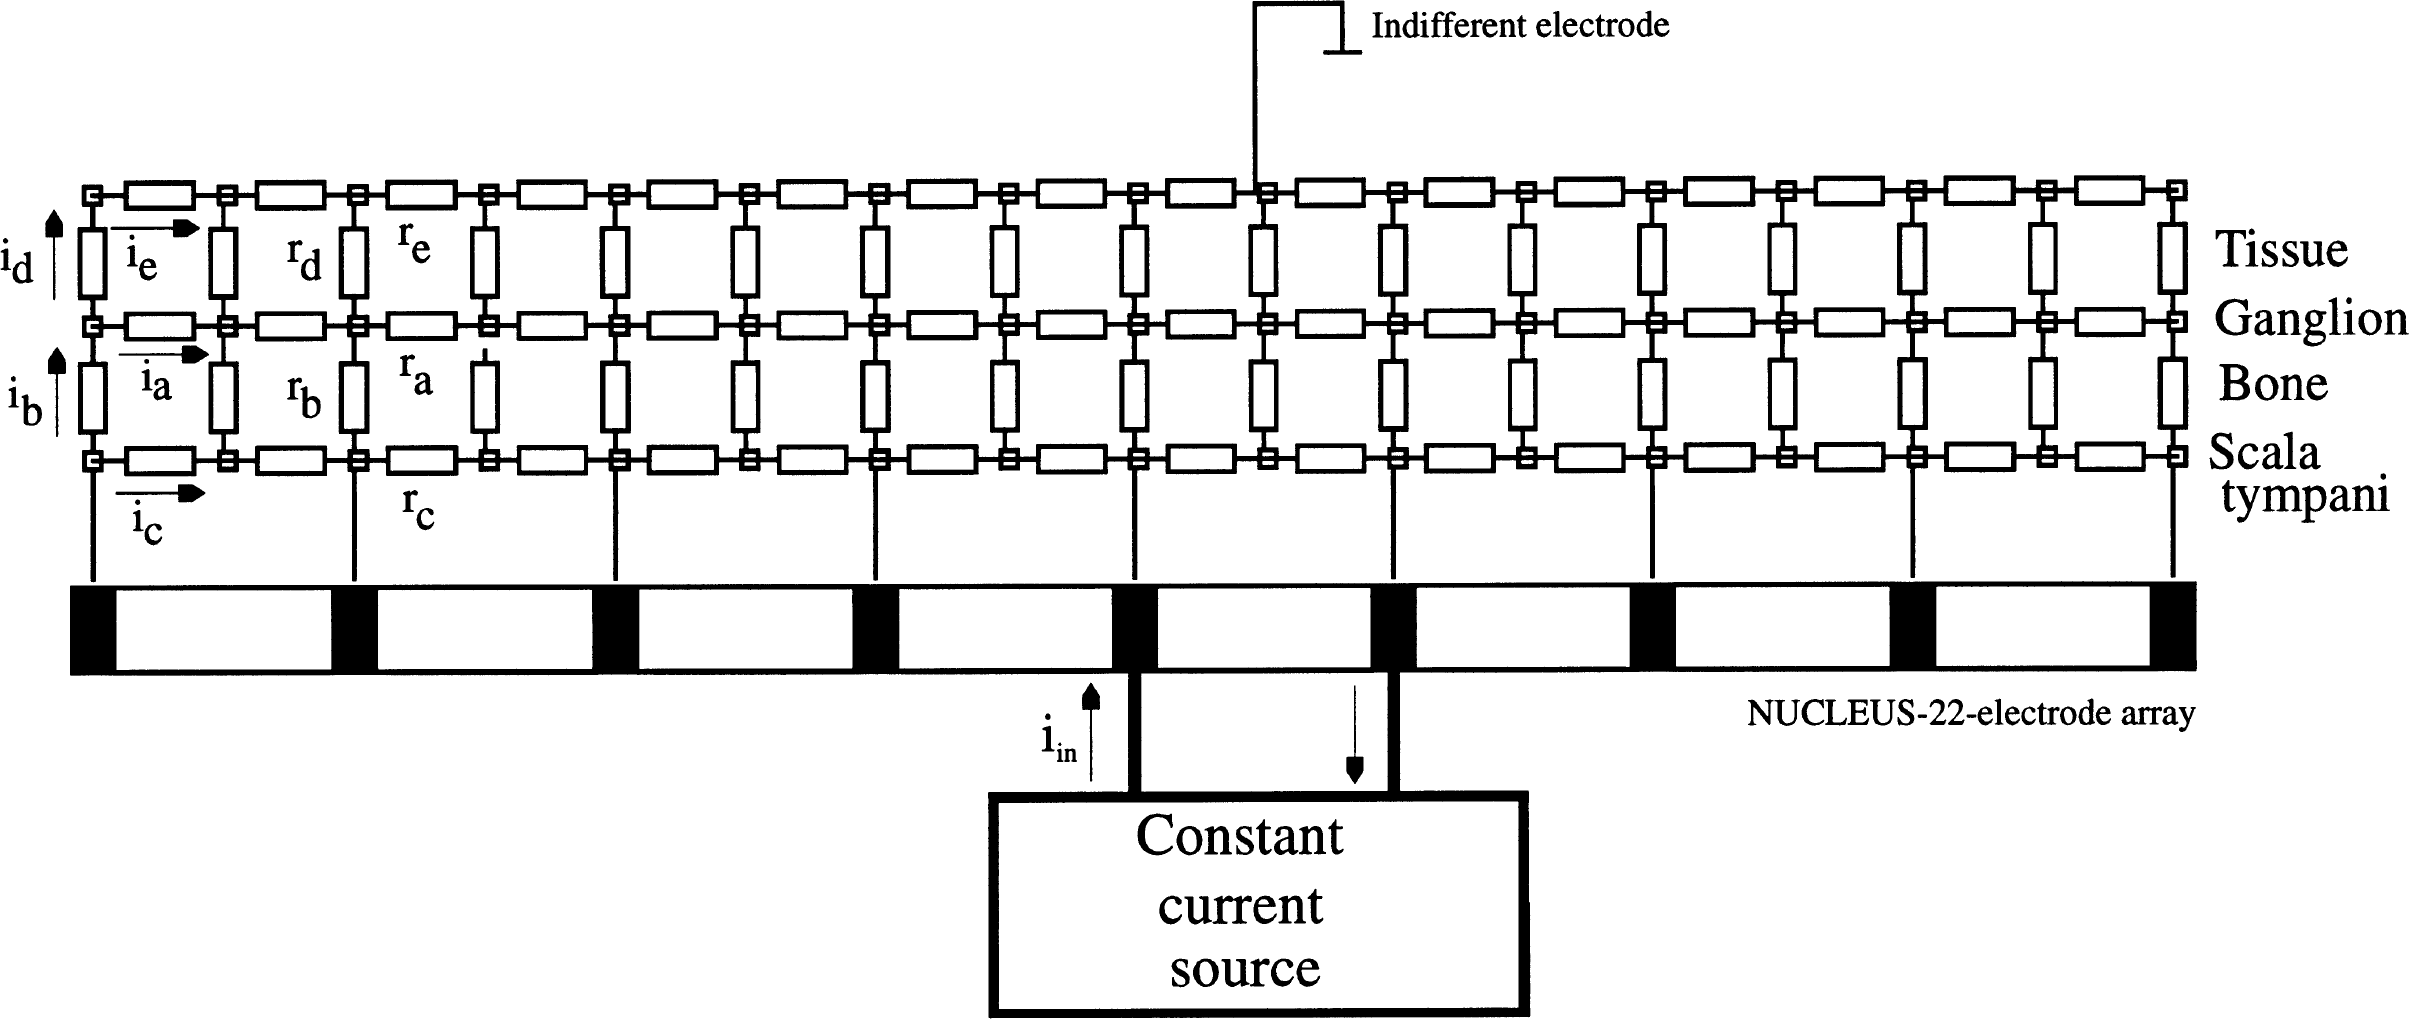
\includegraphics[width=\textwidth]{Background/kral}
	\caption[The Kral model]{The Kral model. (Source: Kral~\cite{kral1998}.
	Copyright \textcopyright{} 1998, Elsevier B.V.)}
	\label{fig:model_kral}
\end{figure}

The primary limitation of the model is that it used a simplified 2D geometry, so
excitable structures near the modiolar wall of the scala tympani were considered
but the nerve tissue in the modiolus was poorly represented. The influence of
other nearby fluid chambers (the scalae media and vestibuli) are not considered,
even though the scala tympani is not perfectly insulated. In addition, it was
comprised of resistive elements only and so did not consider time- and
frequency-dependent effects, which are observed in \invivo{} measurements.

\subsubsection{Vanpoucke \etal{} (2004)}

Vanpoucke \etal{} created an LEM of the cochlea to help interpret data from an
electrical field imaging (EFI) study~\cite{vanpoucke2004identification}. EFI
data were sourced because it is a simple, non-invasive, and rapid measurement
technique. The complete model, shown in Figure~\ref{fig:model_vanpoucke}, is
roughly equivalent to the Kral model in the sense that the network was
structured according to the layers of materials encountered by injected current.
The circuit itself was, however, quite different. It built upon a purely
resistive tissue model introduced in an earlier paper~\cite{vanpoucke2004facial}
and, like the Johnstone model, includes an element representing the total
resistance between the cochlea and the MP reference electrode. Additional
elements were introduced to represent the interface impedance for each
intracochlear electrode contact. All model parameters were then calculated from
experimental measurements using numerical methods.

\begin{figure}
	\centering
	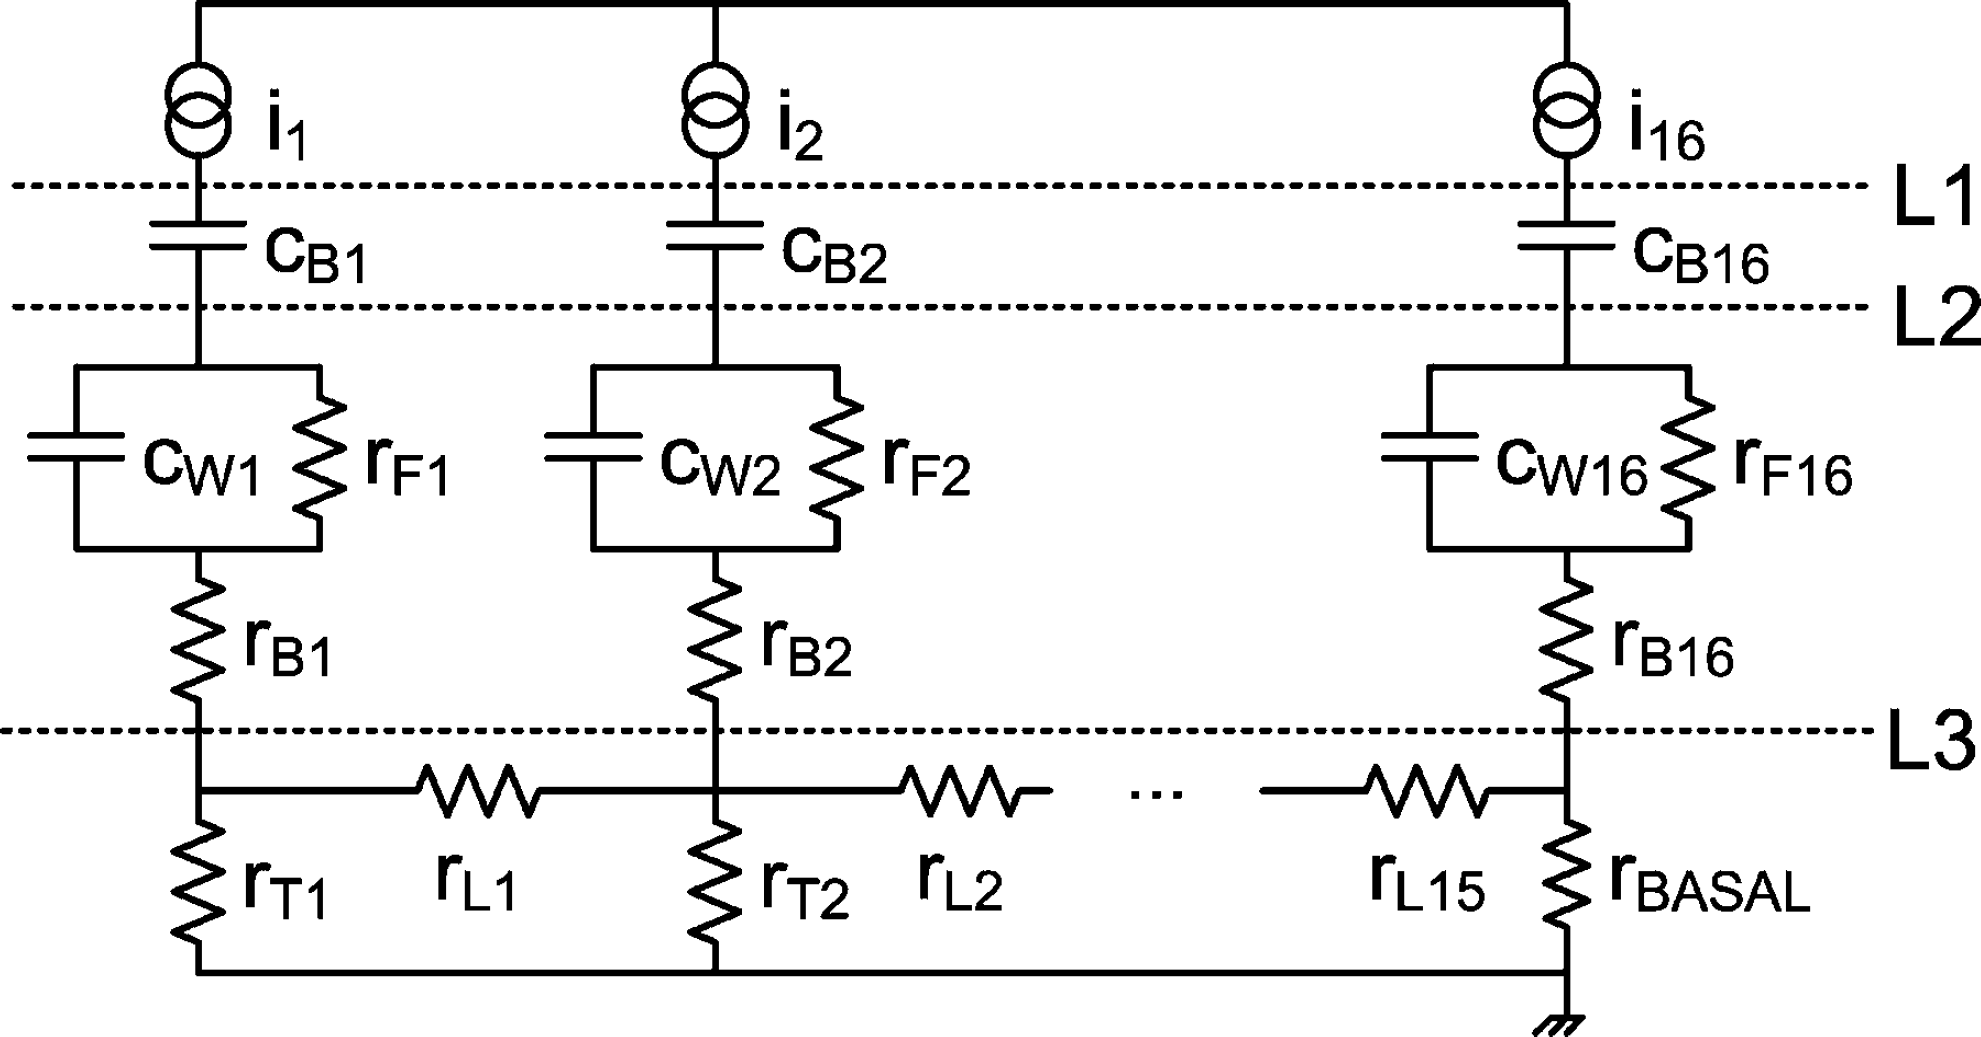
\includegraphics[width=9cm]{Background/vanpoucke}
	\caption[The Vanpoucke model]{The Vanpoucke model. (Source:
	Vanpoucke~\cite{vanpoucke2004identification}. Copyright \textcopyright{} 2004,
	IEEE.)}
	\label{fig:model_vanpoucke}
\end{figure}

The model provided a good match to the EFI data and was able to provide some
insight into the local conductive pathways near the stimulating electrode. There
was some concern about the interpretation of some unanticipated results.
Simplifications made in the construction of the circuit model, such as the use
of a linear tube geometry and the exclusion of the other scalar pathways, are
likely weaknesses in this representation.

% ========================================================================= VCMs

\subsection{Volume Conduction Models}
\label{sect:volume_conduction_models}

% 1987
\subsubsection{Girzon (1987)}

Girzon was one of the first to recognise that representing gross structures as
single nodes or elements was inadequate. He argued that in LEMs, the true 3D
structure of the inner ear is simplified, so some current paths are ignored. The
use of bulk impedance measurements between two points only reveals the
\emph{effective} impedance between them, and does not clearly demonstrate the
spatial pathway traversed by injected current. In addition, the representation
of implanted electrodes as point sources could be inaccurate since the arrays
occupy a substantial volume within the scala and have significantly different
electrical properties relative to the surrounding fluids.

In order to overcome these problems a new type of model was required, leading
Girzon to develop the first VCM of the cochlea (illustrated in
Figure~\ref{fig:model_girzon})~\cite{girzon1987}. By preserving the 3D,
heterogeneous structure of the cochlea, it was hoped that the VCM would be
``electro-anatomically accurate'' and could uncover insights that could not be
revealed using LEMs, such as the true current pathway to ground and the
resultant patterns of neural excitation.

\begin{figure}
	\centering
    \begin{subfigure}[t]{0.4\textwidth}
        \centering
        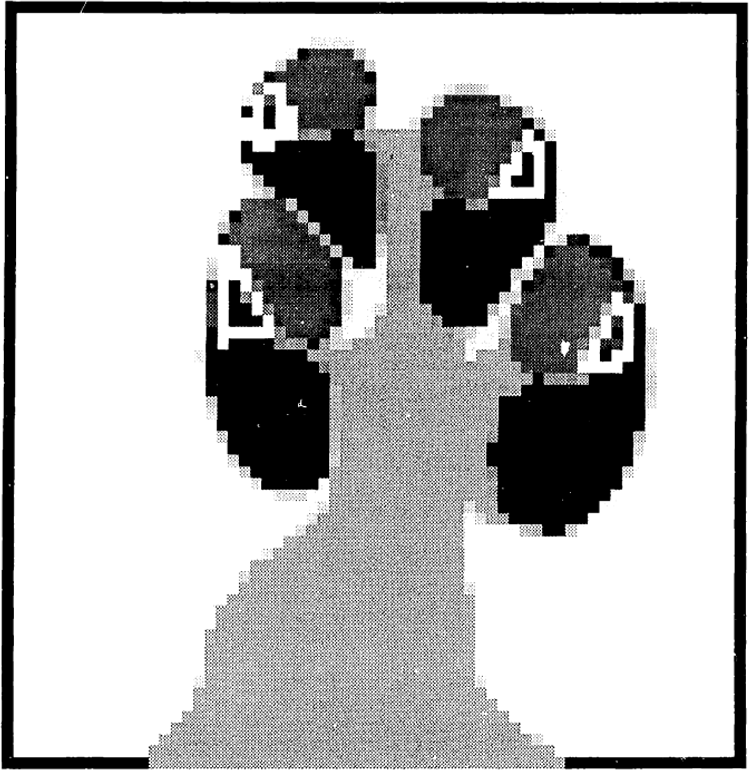
\includegraphics[height=6cm]{Background/girzon_section}
        \caption{ }
        \label{fig:girzon_section}
    \end{subfigure}
    ~~~~
    \begin{subfigure}[t]{0.52\textwidth}
        \centering
        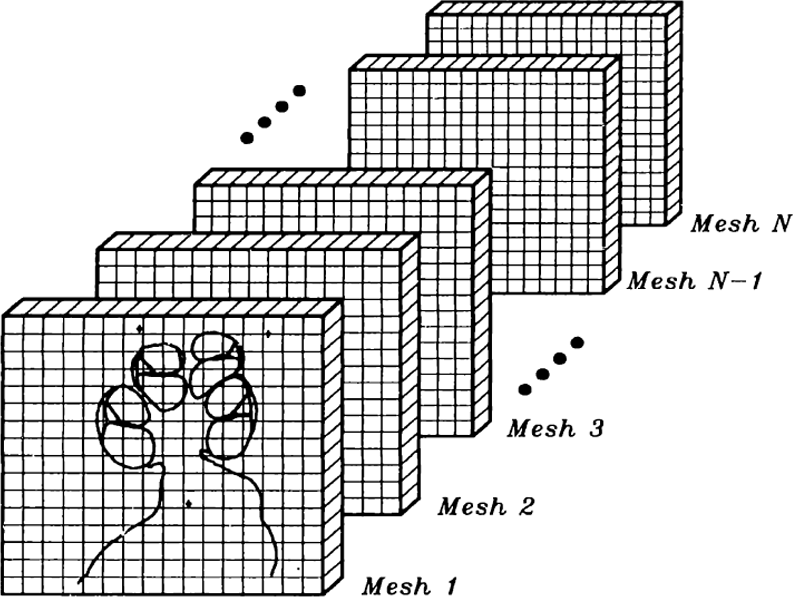
\includegraphics[height=6cm]{Background/girzon_slices}
        \caption{ }
        \label{fig:girzon_slices}
    \end{subfigure}
    \caption[The Girzon model]{The Girzon model. (a) A downsampled mid-modiolar
	section was mapped onto a finite difference grid. (b) The entire model
	consisted of $ N=40 $ slices. (Source: Girzon~\cite{girzon1987}. Copyright
	\textcopyright{} 1987, MIT.)}
	\label{fig:model_girzon}
\end{figure}

The model comprised of a volumetric geometry based on a set of serial sections
of a whole human cochlea. The overall size of the domain was 9.6$ \times $5.76$
\times $7.4 mm. Each section was hand-traced, vectorised, and downsampled to a
128$ \times $128$ \times $40 finite difference mesh
(Figure~\ref{fig:girzon_slices}). Tissue-specific resistivity values were used
as opposed to bulk resistance measurements between arbitrary points. These were
estimated from a variety of sources. Electrical loads were modelled as point
sources within the scala tympani. In terms of boundary conditions, the model was
insulated on all sides (as shown by the black outline in
Figure~\ref{fig:girzon_section}), except for the bottom surface where the
cochlear nerve exited the volume, which was grounded due to its ``electrical
proximity'' to the MP return electrode.

Girzon's VCM was a solid first attempt at creating a true 3D representation of
the electrically stimulated cochlea. He recognised that the key advantage of
this model over LEMs was that it allowed results to be interpreted in a more
accurate spatial context---for instance, the magnitude and direction of field
quantities could be calculated throughout the structure, and indirect current
pathways linking the turns of the cochlea were demonstrated. The model was
successfully used to investigate the effects of several parameters, including
the distribution of electric potential in the scala tympani, the accuracy of
modelling electrodes as point sources, the impact of model resolution, the
effects of material models and properties, and various modes of stimulation.
Validation against \invivo{} experimental measurements showed that the VCM was
superior to transmission line formulations.

Girzon acknowledged that as a first attempt, the model was subject to a number
of drawbacks. Regarding methodology, he suggested that the FEM would have been a
better solution method since it allows for non-uniform element dimensions, but
the FDM was more practical given the compromises between software and hardware
capabilities at the time.

In terms of tissue modelling, the resolution was quite low due to the
constraints in imaging technology. This meant that fine structures such as the
cochlear vasculature could not be reconstructed despite being a highly
conductive pathway. Girzon reasoned that the larger volume of the auditory nerve
made it a more significant path to ground, so the effect of vasculature was
likely to be small. Nonetheless, he called for further investigation of the
blood vessel pathways. The electrical conductivities of several
cochlear-specific tissues were probably also inaccurate since they had not been
measured and were instead based on conductivities of similar tissues that had
been published in the literature. Capacitive effects were ignored on the basis
that the perilymph, nerve, and blood vessels, which were likely to be the
dominant current carrying pathways, had been shown to be primarily resistive at
frequencies of up to 10~kHz~\cite{schwan1957capacitive,geddes1967,spelman1982}.

Finally, Girzon acknowledged that modelling the electrodes as simple point
sources was likely to have overestimated the current densities. He compared the
point source with a small near-spherical volume source and did not find a large
discrepancy in the voltage profile, but only after scaling to the maximum
potential in each trace. The staircase effect would have added to the modelling
error because the spherical current source could not be aligned to the Cartesian
grid. In addition, although grounding the nerve may seem reasonable for LEMs,
prescribing it in a VCM is incorrect since the spatial effects of this boundary
condition are not properly considered. Girzon simply reasoned that it would be
better than grounding all the model boundaries because the potential should be
asymmetric and he did not want to overestimate the voltage attenuation.

% 1990
\subsubsection{Finley \etal~(1987--1990)}

Finley \etal{} improved upon the work of Girzon in a few key areas. Their models
of the human cochlea were based on the FEM, and included volumetric
representations of the implanted electrode array. They started with a simple
two-dimensional (2D) model~\cite{finley1987}, but later extended it into a more
substantial 3D model~\cite{finley1989,finley1990}, shown in
Figure~\ref{fig:model_finley}. These VCMs were used to predict the induced
electric fields within the cochlea tissues, similar to Girzon's work. However,
they also went a step further and coupled it with a neural model to predict the
response of auditory nerve fibres, thereby providing a more complete view of the
CI stimulation process.

\begin{figure}
	\centering
	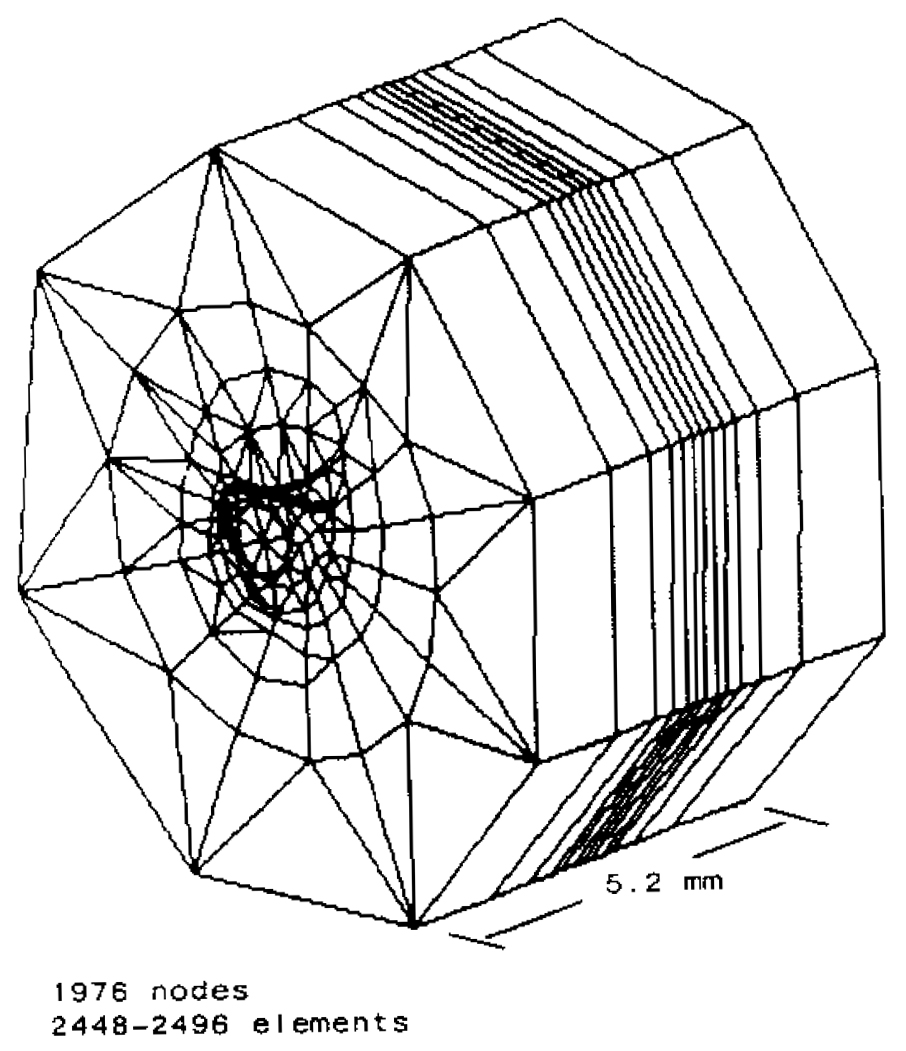
\includegraphics[height=8cm]{Background/finley}
	\caption[The Finley model]{The Finley model. (Source: Finley
	\etal\cite{finley1990}. Copyright \textcopyright{} 1990, Springer.)}
	\label{fig:model_finley}
\end{figure}

The geometry of the Finley model is best described as being extruded. A
histological image of one turn of the cochlea was segmented into various tissues
and discretised, with a higher mesh density in the central regions of the
cochlea. This 2D mesh was extended using prismatic elements to form a slab, and
twelve such slabs were then put together to generate a short, straight section
of the cochlear tube totalling 5.2 mm in length, resembling a short transmission
line model. The slabs closer to the mid-plane of the model were thinner, so the
mesh density was significantly higher in the central regions of the model than
at the periphery. Purely resistive tissue properties were assigned, and a
variety of bipolar electrode configurations were tested. Rattay's activating
function~\cite{rattay1986,rattay1990} was used to predict the likelihood of
excitation along seven neural trajectories.

Finley \etal~found that the model was quite useful for studying various bipolar
electrode configurations. The electrical fields and neural responses were highly
dependent on the arrangement of the source and sink electrodes, as well as the
location of the implanted array within the scala tympani. The greater anatomical
detail and improved (albeit still crude) electrode geometry, made possible
through the use of the FEM and by focusing on only one turn of the cochlea,
helped to increase the accuracy of the predicted electric field distribution
relative to other models.

Nonetheless, omitting the curvature of the cochlea was a step backwards from the
true 3D shape of the Girzon model. The authors indicated that greater anatomical
detail would have been preferred, such as in the lateral wall (i.e.~the spiral
ligament and stria vascularis) and in the modiolus. Unlike the Girzon study
though, the influence of blood vessels was not mentioned at all. The model's
limited spatial domain meant that broadly spreading monopolar fields could not
be considered. It also retained the use of purely resistive material models,
citing Spelman's experimental results~\cite{spelman1982}.

% 1995 (to present)
\subsubsection{Frijns \etal{} (1995--2015)}

The Frijns group is the most active in the field of cochlear modelling. They
have been iterating on their model since 1995, leading to what is rightfully
considered to be the most anatomically realistic representation (see
Figure~\ref{fig:model_frijns_evolution}). The Frijns model is therefore
considered to be the gold standard in this field. As per Finley \etal, it
consists of two coupled sub-models: an electrical VCM, this time based on the
BEM, and a neural excitation model (the generalised SEF model by
Frijns~\cite{frijns1995}), which uses the calculated potential
distribution to predict the electrically-evoked neural response.

\begin{figure}
	\centering
    
    \begin{subfigure}[t]{0.45\textwidth}
        \centering
        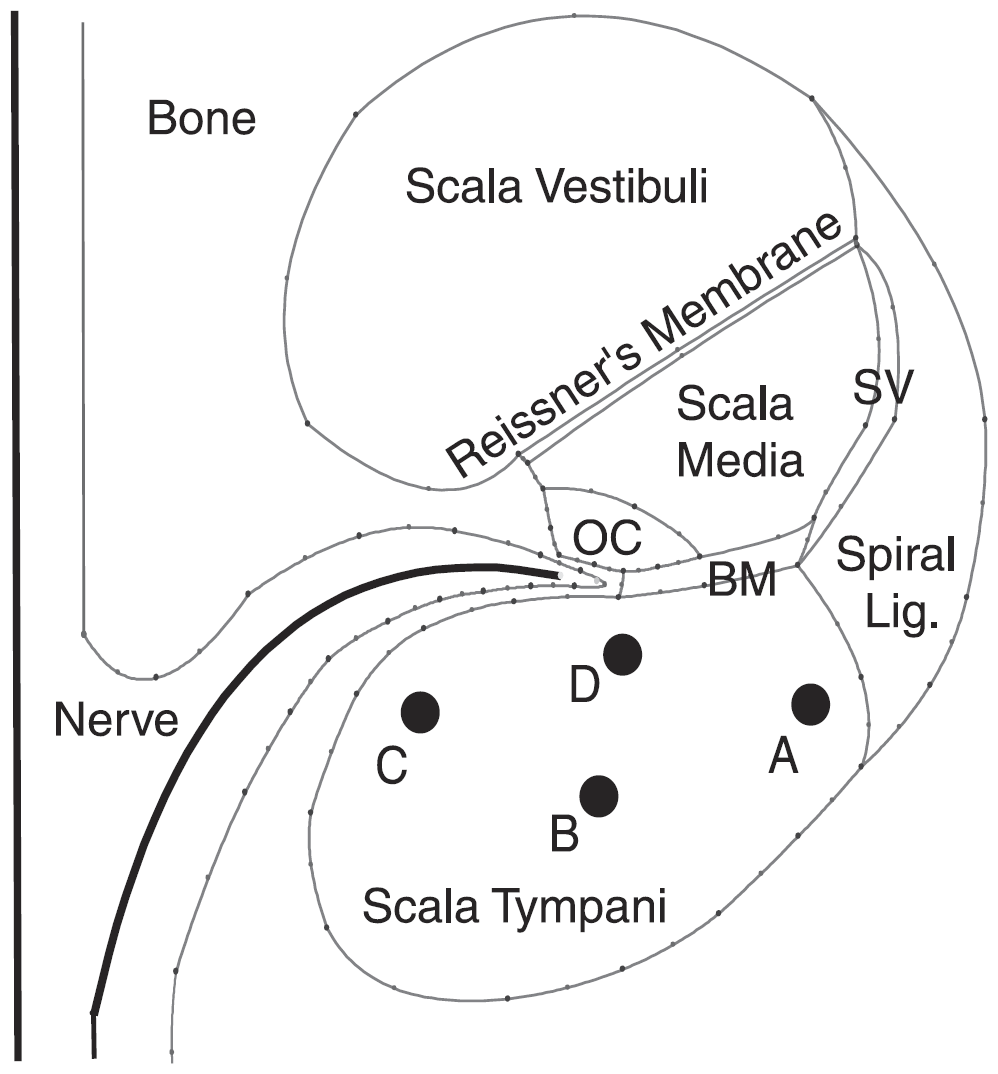
\includegraphics[height=5.1cm]{Background/frijns_spiral_schematic}
        \caption{ }
        \label{fig:frijns_tissues}
    \end{subfigure}%
    ~~~~
    \begin{subfigure}[t]{0.45\textwidth}
        \centering
        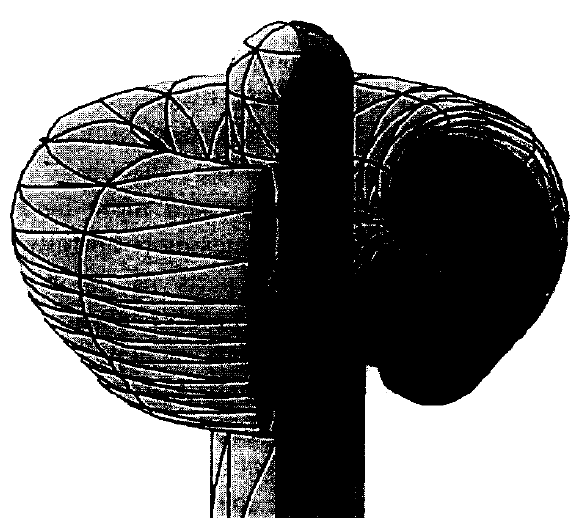
\includegraphics[height=5.1cm]{Background/frijns_rot_mesh}
        \caption{ }
        \label{fig:frijns_rot-1}
    \end{subfigure}%
	\vspace{0.5cm}
	
	\begin{subfigure}[t]{0.45\textwidth}
        \centering
        \includegraphics[height=6cm]{Background/frijns_rot-2_schematic}
        \caption{ }
        \label{fig:frijns_rot-2}
    \end{subfigure}%
    ~~~~
    \begin{subfigure}[t]{0.45\textwidth}
        \centering
        \includegraphics[height=6cm]{Background/frijns_spiral_surf}
        \caption{ }
        \label{fig:frijns_spiral}
    \end{subfigure}%
	\vspace{0.5cm}
    
    \begin{subfigure}[t]{0.45\textwidth}
        \centering
        \includegraphics[height=4.75cm]{Background/frijns_human-1_surf}
        \caption{ }
        \label{fig:frijns_human-1}
    \end{subfigure}%
    ~~~~
    \begin{subfigure}[t]{0.45\textwidth}
        \centering
        \includegraphics[height=4.75cm]{Background/frijns_human-2_surf}
        \caption{ }
        \label{fig:frijns_human-2}
    \end{subfigure}%
    
    \caption[Evolution of the Frijns model]{Evolution of the Frijns model over
    time. (a) Cross-sectional schematic showing the modelled cochlear
    tissues~\cite{frijns2000}; (b) the original axisymmetric
    model~\cite{frijns1995}; (c) the extended axisymmetric
    model~\cite{briaire2000field}; (d) the spiral model~\cite{frijns2000}; (e)
    the original human model~\cite{frijns2001,kalkman2014}; (f) the refined
    human model~\cite{kalkman2014}. (Copyright \textcopyright{} 1995--2014,
    Elsevier B.V.; 2001, Wolters Kluwer.)}
	\label{fig:model_frijns_evolution}
\end{figure}

The initial model~\cite{frijns1995,frijns1996} was based on a histological
section from a guinea pig cochlea~\cite{frijns1995}. An image of the second turn
was digitised, segmented and revolved to form a ``rotationally symmetric'' (i.e.
axisymmetric) toroidal structure (see Figures~\ref{fig:frijns_tissues} and
\ref{fig:frijns_rot-1}). The segmented tissues were embedded in a surrounding
domain of bone. Due to the use of the BEM, the thicknesses of the cochlear
membranes had to be increased to avoid excessive numerical errors, so their
conductivities were magnified proportionally. Conductivity values for the other
tissues were either sourced directly from existing literature or calculated from
published resistance and morphological data. Electrodes were modelled as point
sources located in one of four positions, marked as points A through D in
Figure~\ref{fig:frijns_tissues}. Only BP stimulation was modelled.

Frijns~\etal{} went on to compare this model with existing efforts. They showed
that relative to straight models, such as those of Finley \etal\cite{finley1990}
and Suesserman and Spelman~\cite{suesserman1993}, the calculated potential
fields are significantly different~\cite{frijns1995}, so the assumption of an
unrolled cochlear geometry was invalid. They also showed that Finley~\etal's
omission of the spiral ligament, stria vascularis, and organ of Corti resulted
in an inaccurate representation of the scala media. These three tissue
boundaries act as an insulating layer and help to maintain the endocochlear
potential. Further refinements to the model, including more fine detail,
anisotropic conductivities, and realistic electrode shapes were also discussed.

The guinea pig model was further developed in some later
papers~\cite{briaire2000mesh,briaire2000field,frijns2000}. The most obvious
change to the model was its shape, which became tapered and spiralled up towards
the apex much like a real cochlea. (The helicotrema was not modelled, however.)
This helical shape is important: a comparison of results from a tapered
multi-toroidal model (Figure~\ref{fig:frijns_rot-2}) and the spiral model
(Figure~\ref{fig:frijns_spiral}) showed that the latter more closely matched
experimental work. This reinforced the findings of Ifukube, who had previously
demonstrated the importance of the helical cochlear path on current
distributions~\cite{ifukube1987}. The spiral model also incorporated realistic
electrode geometries based on a variety of clinical designs~\cite{frijns2000}.
Differences due to factors such as electrode spacing and array positioning
within the scala tympani were found. It was therefore made clear that the model
geometry plays a dominant role in volume conduction problems and should ideally
be modelled with the highest feasible accuracy. In terms of boundary conditions,
the model was grounded at infinity~\cite{frijns2000}. No justification was given
in the paper but the choice was presumably made to reflect the far-field MP
return electrode.

In 2001, Frijns \etal{} began directing their efforts towards a human
model~\cite{frijns2001}. Mid-modiolar sections from histological images were
used to define the shape of each turn and the trajectory of the sweep path. They
showed that the differences in geometry (see Figure~\ref{fig:frijns_human-1})
and tissue properties between guinea pig and human cochleae have an impact on
the modelling predictions. As such, even though Miyamoto suggested that guinea
pigs were an appropriate animal model for CI research~\cite{miyamoto1986},
caution must be used when extrapolating \invivo{} or \insilico{} experimental
results to humans. Further refinements to the model have since been made to
investigate specific conditions. These include solving the inverse problem to
better understand the processes underlying ECAPs~\cite{briaire2005}, the removal
of the peripheral processes to model a degenerated physiological
state~\cite{briaire2006}, a comparison of time-dependent stimulation
profiles~\cite{frijns2009simultaneous}, inclusion of the facial nerve to model
ectopic stimulation~\cite{frijns2009stimulation}, and an examination of PA
stimulation techniques~\cite{frijns2011}. The latest revisions of the Frijns
model are highly realistic and are undoubtedly the most comprehensive efforts to
date, not only in terms of the geometry (see Figure~\ref{fig:frijns_human-2}),
but also the trajectory of the neuronal pathways
(Figure~\ref{fig:kalkman_ganglia})~\cite{kalkman2014,kalkman2015}.

\begin{figure}
	\centering
	\includegraphics[width=\textwidth]{Background/kalkman_ganglia}
	\caption[Spatially distributed spiral ganglion cell bodies by
	Kalkman]{Spatially distributed spiral ganglion cell bodies by Kalkman. (a)
	The implementation of the distributed fibre trajectories and spiral
	ganglion cell body locations; (b) the spirally-aligned cell bodies as used in
	previous studies; (c) the updated, spatially distributed cell bodies. This
	enhancement to the Frijns model further improves its anatomically realistic
	geometry. (Source: Kalkman~\etal~\cite{kalkman2015}. Copyright
	\textcopyright{} 2015, Elsevier B.V.)}
	\label{fig:kalkman_ganglia}
\end{figure}

Taken as a whole, Frijns and his co-workers have provided much insight into how
variations in shape affect CI stimulation patterns. This is important because
the geometry of the inner ear differs between species and is also uniquely
shaped for every individual~\cite{escude2006,erixon2009}. No single geometry can
apply equally well to an entire population.

There are still some aspects of the model that could be further improved. For
instance, it has not been shown whether the boundary conditions used in these
models are truly reflective of the \invivo{} situation during MP stimulation. As
with the other VCMs, the effect of the vasculature is simply assumed to be
negligible, so blood vessels have been completely omitted. In addition,
adjustments to both geometry and material properties for the cochlear membranes
were required for accuracy reasons. These are a result of methodological
limitations inherent to the BEM. The models also assume that purely resistive
material models are sufficient in order to simplify the computation.

% 2001
\subsubsection{Hanekom (2001--2015)}

Another FEM of the cochlea was created by Hanekom in 2001~\cite{hanekom2001}.
The model is illustrated in Figure~\ref{fig:model_hanekom} and features an
untapered 3D helical shape totalling 1.5 turns, with cross-sections based on a
combination of photomicrographs from two human cochlea specimens. It
incorporated both a modiolar-hugging and a peripheral track to model different
intrascalar array placements, allowing a variety of bipolar and
pseudo-monopolar electrode configurations to be tested. Like existing
models, the cochlear tissues were embedded in bone; Hanekom opted for a
cylindrical surrounding block of 5.5 mm radius and 10 mm depth oriented parallel
to the mid-modiolar axis, and purely resistive material properties were used.
Hanekom coupled the volume conduction model with the GSEF nerve fibre model,
allowing for some comparisons with the Frijns model.

\begin{figure}
	\centering

	\begin{subfigure}[t]{0.51\textwidth}
        \centering
        \includegraphics[height=6.8cm]{Background/hanekom_section}
        \caption{ }
        \label{fig:hanekom_section}
    \end{subfigure}%
    ~~
    \begin{subfigure}[t]{0.44\textwidth}
        \centering
        \includegraphics[height=6.8cm]{Background/hanekom_mesh}
        \caption{ }
        \label{fig:hanekom_mesh}
    \end{subfigure}%

	\caption[The Hanekom model]{The Hanekom model. (a) Section view of a single
	turn in the model, with tissues as labelled; (b) 3D view of the mesh inside
	the cylinder of surrounding bone. (Source: Hanekom~\cite{hanekom2001}. Copyright
	\textcopyright{} 2001, Wolters Kluwer.)}
	\label{fig:model_hanekom}
\end{figure}

The Hanekom model was able to make conclusions regarding the asymmetry of
potential distributions, as well as the effect of electrode placement on current
spread, thresholds and excitation patterns (including ectopic excitation). It
was later used to model the effect of encapsulation tissue around implanted
electrode arrays~\cite{hanekom2005}.

The main weakness of the model was its geometry. It did not follow a true spiral
trajectory, using instead a series of circular half-turns. The constant
cross-section size was also not realistic---even though the dimensions of the
scala tympani were within 6\% of an average real cochlea, the overall height of
the model exceeded it by some 25\%. Filling and assigning the volume in the
centre of the model to a nerve domain to represent the bundling of axons into
N~VIII ignored the other tissues that also reside in that space, and was not an
accurate depiction of the shape of the nerve trunk. Some tissue thicknesses also
needed to be scaled in order to obtain well-shaped elements. Finally, it did not
incorporate vascular pathways or time-dependent material models.

Since then, the Hanekom group has focused on improving the model geometry by
creating more realistic subject-specific models. This work began with a guinea
pig cochlear model~\cite{malherbe2013}. Human cochlear models have been
developed more recently that also include a low fidelity reconstruction of the
surrounding head to represent the monopolar return path~\cite{malherbe2015}.

\subsubsection{Rattay \etal{} (2001)}

Rattay \etal{} approached the modelling problem from the opposite end. In a
companion paper on neural excitation modelling~\cite{rattay2001neuron}, they
realised that they needed a potential distribution that more closely resembled
the \invivo{} situation in order to properly account for effects arising from
the cochlear anatomy. In response, they constructed a relatively simple FEM
model of the implanted cochlea~\cite{rattay2001model}, which is shown in
Figure~\ref{fig:model_rattay}.

\begin{figure}
	\centering
	
	\begin{subfigure}[t]{0.46\textwidth}
        \centering
        \includegraphics[height=7cm]{Background/rattay_midplane}
        \caption{}
        \label{fig:rattay_section}
    \end{subfigure}%
    ~~~~~
    \begin{subfigure}[t]{0.42\textwidth}
        \centering
        \includegraphics[height=7cm]{Background/rattay_mesh}
        \caption{}
        \label{fig:rattay_mesh}
    \end{subfigure}%
	
	\caption[The Rattay model]{The Rattay model. (a) Section view through the
	mid-modiolar plane; (b) the volume mesh and surrounding bone cube. (Source:
	Rattay \etal~\cite{rattay2001model}. Copyright \textcopyright{} 2001, Elsevier
	B.V.)}
	\label{fig:model_rattay}
\end{figure}

The Rattay model was reconstructed from a single photomicrograph of a
mid-modiolar section of the human cochlea. It was segmented at high resolution
but significantly downsampled, with the outline of the scala tympani comprising
of just seven edges (see Figure~\ref{fig:rattay_section}). Sections were
extrapolated along a fitted spiral path at 30 degree intervals to form a model
with 1.5 turns. An axisymmetric core representing the auditory nerve trunk was
then modelled as a series of stacked cylinders and cones, and the entire
structure was embedded in a cube of bone, as illustrated in
Figure~\ref{fig:rattay_mesh}. Resistivities, predominantly from
Finley~\cite{finley1990}, were assigned to the corresponding tissues, and
capacitive effects were omitted. 0.5 mm diameter spheres were intersected with a
swept 0.4 mm diameter circular profile to approximate a banded multielectrode
array. A 1 V load was placed on the stimulating electrode. All outer surfaces of
the bony cube were grounded, except for the base, where a long prismatic
extension of nerve tissue was used. The neural model in the companion
paper~\cite{rattay2001neuron} was then implemented on the solved VCM.

Rattay \etal{} were able to draw out several different insights. For MP
simulations, it was able to predict that voltage decreased more rapidly in the
basal turn due to the larger size of the scala tympani there, in line with
experimental findings. It also showed that the point of maximum voltage for more
apical fibres lay within the modiolus instead of at the peripheral end. Other
aspects they looked at included BP and quadrupolar stimulation modes,
differences in timing between neurons, and the excitation of degenerated
neurons.

The authors found that the model was not particularly sensitive to the tissue
resistivities used, but acknowledged some uncertainties around material
properties as well as boundary conditions. Also, despite suggesting that the
geometry of the VCM was sufficiently detailed, they understood that the
excitation model predicted a higher probability of activation at strong curves
and mused that more refinement towards the organic geometry of the neural tissue
would therefore be desirable.

% 2004
\subsubsection{Choi \etal{} (2001--2014)}

Choi \etal{} created several models of the cochlea to study shape and location
optimisation of CI electrodes using genetic algorithms. Choi's work on virtual
channels~\cite{choi2009} also showed that several electrode design parameters
had a measurable impact on the efficacy of virtual channel techniques and is a
solid demonstration of how \insilico{} studies can inform electrode designs.

Choi's seminal work only looked at the surface of the electrode~\cite{choi2001},
but subsequent papers also included a model of the cochlear tissues. The
sectional geometry and resistivity values were the same as that of
Hanekom~\cite{hanekom2001,choi2006} (see Figure~\ref{fig:choi_section}), but the
geometry was evolved over time, beginning as a extruded section~\cite{choi2004},
then becoming a semi-circular sweep~\cite{choi2005,choi2009} as shown in
Figure~\ref{fig:choi_mesh}, and finally single-turn circular and spiral
models~\cite{choi2006,choi2014}. Electrode shapes also changed from planar
electrodes~\cite{choi2004,choi2006} to more realistic banded, half-banded, and
ball electrodes~\cite{choi2005,choi2006,choi2009,choi2014}. A neural model was
also implemented as the optimisation criterion. Initially, Rattay's AF was
used~\cite{rattay1990,choi2004}, but the most recent iteration switched over to
the GSEF model~\cite{frijns1995,choi2014}.

\begin{figure}
	\centering
	
	\begin{subfigure}[t]{0.43\textwidth}
        \centering
        \includegraphics[height=6.2cm]{Background/choi_section}
        \caption{ }
        \label{fig:choi_section}
    \end{subfigure}%
    ~~
    \begin{subfigure}[t]{0.53\textwidth}
        \centering
        \includegraphics[height=6cm]{Background/choi_mesh}
        \caption{ }
        \label{fig:choi_mesh}
    \end{subfigure}%
	
	\caption[The Choi model]{The Choi model. (a) Sectional view showing the tissue
	compartments; (b) the tetrahedral volume mesh. (Source: Choi
	\etal~\cite{choi2009}. Copyright \textcopyright{} 2009, Springer.)}
	\label{fig:model_choi}
\end{figure}

Choi \etal{} found that the electrode-tissue interface plays a crucial role in
determining intracochlear impedances~\cite{choi2006}. Their results suggested
that a tapered geometry was important, but the spiral shape was not, in contrast
to Hanekom's findings. The difference may be due to the use of a purely
tetrahedral mesh, instead of Hanekom's hexahedral dominant
mesh~\cite{hanekom2001}. Hanekom's spiral model also included a half-turn of
overlap and was coupled with a different neural model. The group's most recent
work showed that ECAPs predicted by the spiral model correlated qualitatively
with measurements from a CI recipient, but the \invivo{} and \insilico{} results
are plotted on different scales, making comparisons tricky~\cite{choi2014}.

The group also questioned some of the conductivity values used in the model,
which seemed to overestimate results compared to electric field imaging. This
casts some doubt on the work by Vanpoucke~\cite{vanpoucke2004identification} and
Hanekom~\cite{hanekom2001,hanekom2005}, who had used the same values in their
models. Aside from the material properties though, the glaring weakness of the
Choi model is its overly simplified geometry. This was likely required in
order to automate the discretisation stage for their algorithmic testing
methodology.

% 2007
\subsubsection{Tognola \etal{} (2007)}

Tognola \etal{} created a finite element model of the human cochlea to
investigate the relationship between stimulation parameters and the electric
field induced in the cochlear tissues. It highlighted some of the shortcomings
inherent to \invitro{} techniques, as well as the potential promise of
simulation studies for CI optimisation. Their model is illustrated in
Figure~\ref{fig:model_tognola}.

\begin{figure}
	\centering
	\includegraphics[height=7.2cm]{Background/tognola}	
	\caption[The Tognola model]{The Tognola model. (Source:
	Tognola~\cite{tognola2007}. Copyright \textcopyright{} 2007, IEEE.)}
	\label{fig:model_tognola}
\end{figure}

The geometry of the Tognola model was based on the same photomicrograph as the
Rattay model~\cite{rattay2001model}. The cross-sectional boundaries of the
tissues were not as highly simplified as in the Rattay study, but extrapolation
around the spiral path was still performed in 30 degree intervals. Surrounding
the cochlear tissues was a cylindrical domain of bone tissue. In addition, a
full-banded CI array model based on the Nucleus CI24M was inserted into the
scala tympani along an averaged insertion path. Resistivity values for both the
cochlear tissues and the electrode array were sourced from previous
studies~\cite{strelioff1973,finley1990,suesserman1993,gabriel1996b}. Tognola
\etal{} wrote that both MP and BP stimulation modes were tested, but it was not
clear what boundary conditions were imposed for the MP simulation. Finally, the
simulations were compared to measurements in a water tank for validation.

Their results showed differences between the electric field patterns generated
by MP and BP stimulation, with BP stimulation producing steeper gradients as
expected. The \insilico{} BP results also exhibited a qualitatively similar
trend to the corresponding \invitro{} results. However the study was not clearly
linked back to consequences for CI stimulation and offered little insight beyond
what had already been demonstrated.

\subsubsection{Whiten (2007)}
\label{sect:whiten}

The Whiten models~\cite{whiten2007} were the first attempt to reconstruct and
recreate patient-specific responses to CI stimulation. Two VCMs of two different
CI recipients were generated, each of which was compared to similar population
data, as well as archival data (intracochlear potentials, psychophysical
thresholds, and ECAP recordings) collected from each patient during life. This
was crucial for properly validating the higher-level \insilico{} predictions of
the models.

The model geometries were reconstructed from serially-sectioned images of the
implanted cochleae after death. Image resolution was $ 17.8 \times 17.8 \times
20~\upmu $m for the Ineraid model, and $ 16.8 \times 16.8 \times 40~\upmu $m for
the Nucleus model. In this way, the detailed pathology of each cochlea, the
locations of nearby structures in the temporal bone (namely the facial and
vestibular nerves, the vestibular labyrinths, and the carotid artery, which may
all be important during monopolar stimulation), and the true trajectory of the
implanted electrode arrays was reflected in the digital models. The Nucleus
model is shown in Figure~\ref{fig:model_whiten}. A generalised model was also
created from one of the data sets. Purely resistive material properties were
assigned to the tissues, but curiously the values used were from older papers
and not specific to the human cochlea~\cite{geddes1967,peterson1978}. The models
were solved using the FDM and coupled with a modified version of McNeal's single
nerve fibre model~\cite{mcneal1976} to predict activation patterns. This was in
turn used to predict extracellular current flow along each fibre, and finally
the expected ECAP waveforms at each electrode.

\begin{figure}
	\centering
	
	\begin{subfigure}[t]{0.42\textwidth}
        \centering
        \includegraphics[height=5cm]{Background/whiten_1-segmentation}
        \caption{ }
        \label{fig:whiten_segment}
    \end{subfigure}%
    ~~
    \begin{subfigure}[t]{0.42\textwidth}
        \centering
        \includegraphics[height=5cm]{Background/whiten_2-anatomy}
        \caption{ }
        \label{fig:whiten_anatomy}
    \end{subfigure}%
    \vspace{4mm}    
    \begin{subfigure}[t]{0.42\textwidth}
        \centering
        \includegraphics[height=5cm]{Background/whiten_3-nerves}
        \caption{ }
        \label{fig:whiten_nerves}
    \end{subfigure}%
    ~~
    \begin{subfigure}[t]{0.42\textwidth}
        \centering
        \includegraphics[height=5cm]{Background/whiten_4-array}
        \caption{ }
        \label{fig:whiten_array}
    \end{subfigure}%
    
	\caption[The Whiten model]{The Whiten model of an implanted Nucleus array. (a)
	A segmented slice of the human cochlea; (b) 3D view of the tissue surfaces; (c)
	a mid-modiolar view of the nerve tissue and fibre tracks; (d) the segmented
	electrode array. (Source: Whiten~\cite{whiten2007}. Copyright
	\textcopyright{} 2007, MIT.)}
	\label{fig:model_whiten}
\end{figure}

Whiten used the models to investigate the effect of various parameters on
current flow, neural excitation, and ECAPs, with mixed results. He found that
the detailed anatomy of the cochlea and the resistivities of the materials
(particularly bone and the cochlear fluids) were the primary factors driving
\insilico{} current flow predictions. For instance, a homogeneous model
(analogous to using an analytical solution assuming a uniform resistivity)
predicted a vastly different pattern of current spread than the heterogeneous
model, verifying the need for VCMs. Finer anatomical details also affected
current flow, but the results were generally small and localised. The peripheral
anatomy (namely the facial nerve and the vestibular system) is likewise expected
to have minimal impact. However, encapsulation tissue is an important factor,
and models of chronic CI stimulation that include this should account for the
spatial distribution of the scar tissue. ECAP predictions were not perfect but
the correlation with \invivo{} data was surprisingly solid. It was noted,
however, that several underlying assumptions were likely to be violated, so the
results are either insensitive to those assumptions or they may be falsely
positive. Predictions of psychophysical data from the implant recipients were
considered less successful, which might be expected considering the compounding
of modelling errors through multiple layers of abstraction.

Some aspects of the Whiten study are likely candidates for improvement. The
geometry is not particularly detailed, and the choice of resistivity values is
questionable. Whiten also concluded that further work is required to determine
appropriate boundary conditions and exit pathways under MP stimulation. Finally,
the assumption of longitudinal current flow directions and measurements brings
to mind the older LEM transmission line models and may not be appropriate. The
promise of detailed (and in this case, patient-specific) current flow
visualisation was poorly realised, though admittedly this is true for all models
to date.

\subsubsection{Saba (2012)}

Saba created a few models to investigate the spread of voltage within the
cochlea, the consequences of current-steering techniques, and methods for
improving the power efficiency of CI devices~\cite{saba2012}. His coiled model,
shown in Figure~\ref{fig:model_saba}, was based on a mid-modiolar section from
Zakis and Witte~\cite{zakis2001} that was scaled to size according to dimensions
from various literature sources. The 3D geometry was approximated using lofted
cross-sections and guide curves in a computer-aided design (CAD) program. An
electrode array model based on a data sheet of the Cochlear Nucleus 24 Contour
and Contour Advance electrode arrays was similarly constructed for this study.
Resistivity data was taken from previous modelling
efforts~\cite{finley1990,hanekom2001,briaire2000mesh,rattay2001model}.

\begin{figure}
	\centering
	\includegraphics[height=5.5cm]{Background/saba_3D}	
	\caption[The Saba model]{The Saba model. (Image adapted from
	Saba~\cite{saba2012}. Copyright \textcopyright{} 2012, Rami Saba.)}
	\label{fig:model_saba}
\end{figure}

Once again, the spiral geometry of the cochlea was shown to be important to the
voltage distribution. Saba concluded that this was a driving factor behind the
inter-patient variability in CI performance. It is worth bearing in mind,
however, that the geometry of the Saba model is simplified and does not include
all known cochlear tissues. The modelling results also suggested that current
focusing methods such as PA stimulation were less effective when considering
effects at the level of the spiral ganglion, but could be optimised at a high
power cost. Unfortunately, the criterion used were purely electric field
quantities and were not properly tied back to neural excitation. Likewise, he
found that placing a ball return electrode in the modiolus would reduce CI power
consumption, but he does not consider the surgical practicality of doing so nor
the effect on the auditory nerves (in terms of ectopic stimulation or
electrochemical safety) near the proposed return. His final key finding was that
power harvesting is not feasible for contemporary CI systems due to insufficient
efficiency.

% Summary table of the models?

\section{Research Questions}
\label{sect:research_questions}

The state-of-the-art has advanced significantly in comparison to the
pioneering studies. Nevertheless, there are some areas where \insilico{}
bioelectric models of the cochlea can still be improved. At the core of the
problem is a hitherto incomplete investigation of the assumptions used to
generate the models, which has led to a lack of consensus on some modelling
issues and apprehension by CI researchers, especially those on the clinical end
of the spectrum, to trust modelling predictions. These outstanding issues must
be resolved because neural excitation models depend on the field distribution
predicted by VCMs. If the assumptions on which VCMs are based are invalid, then
the predictions of neural activity in coupled models are similarly moot.

% Need to make sure model are trustworthy. Are models accurate? How to improve
% accuracy?

% No consensus on boundary conditions. Mention of blood vessels but not in
% models. Time-frequency effects? All appear to be loose ends. Is the additional
% effort worthwhile?  There has not been a strong focus on the effect of
% modelling assumptions on the underlying physics, most skip straight to neural
% models. We focus on the physics instead of the psychophysics, which are
% further removed, for this thesis.

There are three key assumptions that this thesis attempts to address. The first
is how best to impose boundary conditions for models of MP stimulation. Boundary
conditions are a core input parameter in modelling studies and are particularly
important in MP simulations because the return path to the extracochlear
electrode lies outside the physical domain of the model itself. The lack of
consensus for prescribing boundary conditions is not ideal for practitioners and
detracts from the appeal of models to clinicians. Different boundary conditions
will affect the exit paths taken by injected current, and the significance of
this impact on results in the neural structures has not yet been studied. The
most accurate approach would be to create a multiscale model that includes the
entire head~\cite{tran2015}, but this is not feasible in most cases. Therefore,
the next best option would be to identify a boundary condition that can be
applied within the model domain and that closely replicates the current flow
patterns of the whole head situation.

The second assumption is that the vascular pathways in the cochlea play a
negligible role in volume conduction. Early studies suspected that the low
resistivity of blood and the pervasiveness of the vascular network makes them an
important conductive pathway~\cite{vonbekesy1951,johnstone1966,girzon1987}. All
VCMs to date have, however, ignored their presence despite the lack of
definitive evidence for their omission. Those that discussed this issue assumed
that the vessels would have minimal impact on the global current pathways
because they occupy a relatively small volume, but this measure alone fails to
consider the proximity of the modiolar vessels to the stimulating
electrodes---which magnifies the effect on the overall current paths as shown by
Baker~\cite{baker1989}---and the trajectory of the vessels through key
structures such as the modiolar bone and the nerve trunk.

Last is the quasi-static assumption on which all existing VCMs are predicated.
This is perhaps their most glaring weakness because it is well known from
experimental work that the \invivo{} responses---especially those in neural
tissue---are time-dependent. There are several reasons VCMs have applied the
quasi-static assumption. Firstly, there is a lack of data on the
frequency-dependent resistivities and permittivities of cochlear-specific
tissues. Secondly, at the relatively low fundamental frequency of CI input
pulses, resistivity values for other bodily tissues are somewhat invariant and
permittivity only plays a minor role~\cite{gabriel1996b}. Thirdly, voltage
response measurements within the scala tympani by Spelman~\cite{spelman1982}
demonstrated minimal phase lag, and this is often cited as justification for
creating stationary models. However, only frequencies up to 12.5 kHz were
tested, which ignores the high frequency components of clinically used square
waves, and measurements in other cochlear tissues may exhibit a more pronounced
effect due to higher tissue permittivities. The final reason is that model setup
and solution is much simpler under quasi-static conditions, with the lower
computational effort enabling substantially faster simulation times.

In addition to these, there is also a need to better visualise the underlying
physics of the stimulated cochlea. Many models relate the simulation results
directly to psychophysical measurements, providing no insight into the physical
relationships that might be used to improve the design of electrode arrays.
The models that do talk about electric current streamlines when discussing
charge movement through the cochlea have not provided illustrations of these
streamlines through 3D space. An intuitive representation of these physical
quantities would therefore aid in promoting a deeper understanding of the
factors affecting CI stimulation in a wider audience and may lead to new and
useful insights for future array designs.
				% Chapter 2 & 3: Background
	\setstretchnormal

\chapter{Model Development}
\label{sect:modelling}

% Textbox
\begin{center}
	\begin{tcolorbox}[title=\boxtitle]
		\begin{itemize}[leftmargin=*,labelindent=2ex,labelsep=1.5ex,itemsep=0pt,parsep=0pt]
			\item How should the bioelectric models be created?
			\item What are the required inputs?
			\item What specific steps were followed to create the models?
		\end{itemize}
	\end{tcolorbox}
\end{center}

% This chapter documents how the models in this thesis were created. It begins
% with a preliminary discussion on the available \textit{in silico} numerical
% methods and the rationale for choosing the finite element method. This is
% followed by a survey of the required inputs, and a workflow for combining all of
% these inputs into a virtual representation of the implanted cochlea. An initial
% proof of concept workflow was evolved into a more robust version that was then
% implemented on two volumetric datasets: a guinea pig cochlea from a stack of
% sTSLIM images, and a human cochlea from a stack of microCT images. These models
% are then used for the investigations detailed in chapters 5--7.

%% ========================================================== Modelling Approach

\section{Introduction}

The overarching goal of this thesis is to determine how volume conduction models
(VCMs) of the cochlea can be improved. An accurate VCM would allow a better
spatial understanding of the cochlear implant (CI) system to be obtained, and
for the research questions detailed in \S\ref{sect:research_questions} to be
answered. To achieve these outcomes, it was important to develop and implement a
methodology that was robust, flexible, and efficient, which was not a trivial
task given the challenges in model
creation~\cite{briaire2000mesh,whiten2007,potratz2010,saba2012}. Therefore, a
number of solution methods, software packages, and input parameters were
critically considered. The initial workflow was progressively evolved to
overcome a number of different computational issues, and to represent the data
more intuitively so that implications could be inferred and conclusions easily
drawn.

This chapter documents the groundwork required to prepare the models of the
thesis for more in depth simulation studies. It covers the foundational work
that was performed to get the models into COMSOL, such as the imaging,
reconstruction and discretisation of the spatial domain, and consideration of
other required inputs such as material properties, loading, and boundary
conditions. The extensive documentation is intended to provide some guidance for
others looking to undertake development of a cochlear VCM. Details of the actual
analyses, including simulation results, are provided in the subsequent chapters.

\section{Preliminary Considerations}

\subsection{Modelling Workflow}

\subsubsection{Generalised Pipeline}

The typical flow of data when creating a VCM has been summarised by both
MacLeod~\cite{macleod2009} and Lau~\cite{lau2011}. The model development
workflow used for this project was informed by these procedures and is
illustrated in Figure~\ref{fig:workflow_general}.

\begin{figure}
	\centering
	\includegraphics[width=11.8cm]{Methodology/workflow_general}
	\caption[Overview workflow schematic]{Overview workflow schematic, summarising
	the key objectives of each stage and the flow of data along the pipeline.}
	\label{fig:workflow_general}
\end{figure}

The first stage of the workflow is creating the model geometry, and there are
two main alternatives to achieve this. A realistic reconstruction of the
cochlear anatomy can be segmented from volumetric scan data, but it is also
possible to use a few cross-sectional images in conjunction with computer-aided
design (CAD) software to generate a cochlea-like shape. In either case, a solid
model of the cochlea is combined with an intracochlear electrode array that is
virtually inserted into the scala tympani. The model is then meshed and analysed
using a numerical method, and various results of interest are exported,
processed, and interpreted by the researcher. Finally, the \insilico{} results
are compared with \invivo{} validation data to demonstrate their correlation
and to check whether the overall level of error is acceptable.

One of the main considerations when developing the workflow was the modularity
of the pipeline. A monolithic program that encompassed the entire workflow could
be ideal for ensuring format compatibility and reducing the number of programs
that needed to be learned. However, it would also be useful to be able to
interface with independent programs and take advantage of specific tools or
functions that were more convenient or better implemented. Software-agnostic
formats for the various data types along the pipeline would facilitate this
flexibility and the potential for a more refined outcome. Of course, it would
need to be balanced against the time and financial costs of integrating more
programs---the latter could become especially prohibitive if commercial
licencing agreements are required.

\subsubsection{Effect of Uncertainties}

VCMs require a number of data inputs as part of the \insilico{} reconstruction.
These can be classified into four categories as shown in
Table~\ref{table:model_inputs}. Clearly, the quality of the input data
influences the accuracy of the final model, but these data are difficult to quantify
accurately due to the biological nature of the system.

\begin{table}
	\centering
	\sffamily
	\small
	
	\caption[Data inputs required for volume conduction modelling]{Data inputs
	required for volume conduction modelling.}
	\label{table:model_inputs}
	
    \begin{tabular}{l l}
	\toprule
	\textbf{Input}			& \textbf{Description} \\
	\midrule
	
	Geometry				& The shape of the structures within the region of interest \\
	Material properties		& The resistivity and permittivity of each structure due to \\
							& \tableindent its physical composition \\
	Loads					& The electrical forces to which the system is being subjected \\
	Boundary conditions		& The conditions for physical compatibility at the boundaries \\ 
							& \tableindent of the modelled domain \\
	\bottomrule
	\end{tabular}
		
\end{table}

Of the four input types listed, only the electrical loads are well defined since
these are controlled via the programming of the implant. The shape of the cochlea
differs from one individual to the next, making it difficult to define an
``average'' or ``median'' cochlea. Erixon's work with corrosion
casts~\cite{erixon2009} provides a good sense of this variability. In terms of
the material properties, the conductivities of the cochlear tissues have been
measured experimentally, but the precision of each measurement varies and the
values can also differ between individuals. Cochlear-specific tissue
permittivities have not been measured at all. The kinetics at model boundaries,
which are especially important in monopolar simulations, depend on the physical
scope of the model, and to date have largely been based on assumptions with no
consensus amongst practitioners. Combined with the segmentation, discretisation,
and numerical errors inherent in computational modelling, these uncertainties
adversely affect the reliability of modelling results. Controlling the sources
of error is therefore an important consideration.

Consulting engineer David Beneke encapsulated these concerns neatly as follows:

\begin{verse}
	\textit{
		``The art of finite element analysis is modelling}
		
	\begin{quote}
		\indent \textit{materials we do not wholly understand,} \\
		\indent \textit{in shapes we cannot precisely form} \\
		\indent \textit{so as to withstand forces we cannot properly assess,}
	\end{quote}
	
	\textit{		
		in such a way that the analyst is confident in the design with the public
		having no reason to suspect the extent of one's ignorance.''}

	\vspace{4mm}

	\raggedleft{
		--- David Beneke~\cite{beneke2014}}
\end{verse}

With this in mind, there are several avenues for inspiring trust in the
\insilico{} results. Firstly, a critical review of the model inputs in
conjunction with sensitivity studies will reveal the degree of uncertainty; if
the level of uncertainty is low or the system is insensitive to the input, then
the data may be used with some confidence. Secondly, modelling errors can be
minimised by using a robust workflow and by taking care during each stage of the
development pipeline. Thirdly, validation of the model via comparison with
independently obtained \invivo{} measurements will ensure that the \insilico{}
predictions are reasonable and within expected real-world limits.

The issues surrounding each input type are discussed presently.

\subsection{Geometry and Imaging}
\label{section:imaging}

Unlike typical engineering structures, the geometry of living organisms is
incredibly complex, and very few organs exhibit true planar or rotational
symmetry~\cite{miller1990}. Defining the physical domain is therefore a
significant challenge, especially given the intricate shape and inaccessible
location of the cochlea. Several different aspects needed to be considered with
regards to reconstructing the cochlea \insilico.

\subsubsection{Subject-Specific versus Generalised Modelling}

The first was whether to create a subject-specific model or a generalised one.
Examples of subject-specific models are those by Girzon~\cite{girzon1987},
Whiten~\cite{whiten2007}, and Malherbe~\cite{malherbe2013,malherbe2015}. In
these models, the geometry is typically obtained from volumetric scans of the
region of interest for a particular individual. If the image stack is of
sufficient resolution, a highly detailed and accurate reconstruction can be
generated. The model would only be directly applicable to the scanned
individual, but insights may be extrapolated (with care) to a more general
population, especially if the geometry does not deviate too far from the mean.

In contrast, generalised models are designed with the goal of representing an
``average'' or ``median'' cochlea without replicating any particular individual.
Generalised models have been created with a variety of means; typically, a
cross-sectional histological image of a real cochlea is swept along an average
path that is either
linear~\cite{finley1990,frijns1995,choi2001,saba2012,wong2012},
circular~\cite{choi2004,frijns1995}, or
helical~\cite{frijns2001,hanekom2001,rattay2001model,tognola2007,saba2012,kalkman2014}
in shape. They can be easier to manipulate during the modelling phase than
subject-specific models because the shape is described by a known equation, so
they can be parametrised and fitted to different patients (inevitably with some
degree of error). The increased tangential smoothness also makes them easier to
discretise. However, they are generally less realistic, particularly at the
basal and apical extremes where the shape deviates from the rest of the
cochlear spiral.

A subject-specific model was deemed better for this project because of the
potential for greater realism, and because the complex distribution and
convoluted paths of the cochlear blood vessels would be difficult to reconstruct
accurately using an equation-based model. The findings would also be more
relevant to the longer-term trend in the industry towards building customised
models for surgical planning and predicting patient outcomes.

\subsubsection{Selection Criteria for Image Data}

Obtaining suitable volumetric scan data for a subject-specific model was a
significant challenge because the goals of the project required fine anatomical
details to be part of the final model. These structures are extremely
small---for instance, Reissner's membrane, the basilar membrane, and the stria
vascularis in the guinea pig are roughly 1.7 $ \upmu $m, 4 $ \upmu $m, and 40 $
\upmu $m thick, respectively~\cite{frijns1995}; the diameters of the smaller
cochlear blood vessels are similar in scale, as shown in
Table~\ref{table:vessel_diams}.

\begin{table}
	\centering
	\sffamily
	\small
	
	\caption[Measurements of cochlear vessel diameters in man]{Measurements of
	cochlear vessel diameters in man.}
	\label{table:vessel_diams}
	
	\begin{tabular}{l c l}
		\toprule
		\textbf{Blood vessel} 	& \textbf{Lumen diameter}				& \textbf{Source}\\
								& \textbf{($ \boldsymbol{\upmu} $m)}	& \\
		\midrule
		
		Radiating arterioles & & \\
		\tableindent``Vascular spring-coils"	& 20--40	& Scuderi and Del Bo~\cite{scuderi1952}\\
		\tableindent Spiral lamina				& 30--40	& Charachon~\cite{charachon1961}\\
		
		Arterio-venous anastomoses				& 15--20	& Charachon~\cite{charachon1961}\\
		
		Capillaries & & \\
		\tableindent Stria vascularis			& 7			& Charachon~\cite{charachon1961}\\
		\tableindent Scala vestibuli			& 5-10		& Charachon~\cite{charachon1961}\\
		\tableindent \textit{(Unspecified)}		& 5--10		& Axelsson~\cite{axelsson1968}\\
		\tableindent 							& 6--12		& Mondy~\cite{mondy2009thesis}\\
		
		Vessel of the basilar membrane			& 10--20	& Charachon~\cite{charachon1961}\\
		Collecting venules						& 10--17	& Charachon~\cite{charachon1961}\\
		\bottomrule
	\end{tabular}
\end{table}

Visualising individual parts is relatively straightforward---the scalae can be
discerned easily~\cite{poznyakovskiy2008,potratz2010}, and fine structures can
also be resolved provided sufficient imaging resolution~\cite{braun2012}---but
the requirements for accurate mesh generation are substantially more
stringent~\cite{poznyakovskiy2008}. A VCM requires that the various component
structures be connected throughout the domain regardless of the complexity of
the interfacing regions. Structural discontinuities (e.g. holes in the
membranes, gaps between parts, or disconnected vessels) and deformations (e.g.
ripples in smooth membranes, image artefacts) will adversely affect the
reconstructed geometry~\cite{briaire2000mesh,poznyakovskiy2008,johnson2014}.

The ideal dataset would therefore possess the following attributes. Firstly,
given the thinness of the membranes and the small size of the vasculature, the
image resolution must be of the same order as these fine structures to maximise
opportunities for feature extraction. The most detailed dataset available should
be used since the data could be downsampled if computational requirements are
excessively high, but cannot be upsampled to provide enhanced detail of
pre-existing features~\cite{schimpf1998}. Technical limitations related to the
specific imaging technique and the need to maintain the entire cochlea within
the field of view will enforce an upper limit on the attainable resolution for
any given sensor size~\cite{poznyakovskiy2008}.

Secondly, the contrast and clarity of the dataset were also important. Since the
model was to contain a large number of different tissue types in the final
reconstruction, each tissue had to be visible and recognisable in the image
stack, ideally with distinct boundaries to facilitate the segmentation process.
Imaging artefacts and noise in the scans were similarly undesirable because
they hinder accurate reconstruction.

Lastly, the availability of each technique was a key determinant because the
scans were to be sourced from third parties with the necessary equipment and
expertise. This would ensure that the image stacks from any chosen modality
had the best chance of fulfilling these desired attributes.

\subsubsection{Comparison of Imaging Modalities}

Multiple options were considered for this project, namely \emph{computed
tomography} (CT), \emph{magnetic resonance imaging} (MRI), \emph{histological
serial sectioning}, and \emph{(laser) light-sheet fluorescence microscopy}
(LSFM). Examples of each modality are provided in
Figures~\ref{fig:imaging_comparison_human} and \ref{fig:imaging_comparison_gp}
for human and guinea pig cochleae, respectively.

\begin{figure}[p]
	\centering
	
	\begin{subfigure}[t]{0.49\textwidth}
        \centering
        \includegraphics[height=4.9cm]{Methodology/ct_human_postnov}
        \caption{CT}
        \label{fig:ct_human}
    \end{subfigure}%
    ~%
    \begin{subfigure}[t]{0.49\textwidth}
        \centering
        \includegraphics[height=7cm]{Methodology/mri_human_silver}
        \caption{MRI}
        \label{fig:mri_human}
    \end{subfigure}\\%
    \vspace{1em}%
    \begin{subfigure}[t]{0.49\textwidth}
        \centering
        \includegraphics[height=6.5cm]{Methodology/histo_human_rattay}
        \caption{Histological section}
		\label{fig:histo_human}
    \end{subfigure}%
    ~%
    \begin{subfigure}[t]{0.49\textwidth}
        \centering
        \includegraphics[height=4.9cm]{Methodology/tslim_human_johnson}
        \caption{LSFM}
        \label{fig:opfos_human}
    \end{subfigure}%
    
	\caption[Comparison of imaging modalities for the human cochlea]{Comparison of
	imaging modalities for the human cochlea. MicroCT and high resolution MRI are
	shown here; clinical counterparts would have significantly lower resolution.
	Note the different types of imaging artefacts and the variations in
	resolution and clarity. (Sources: (a)~Postnov~\cite{postnov2006}, Copyright
	\textcopyright{} 2006, Taylor \& Francis; (b)~Silver~\cite{silver2002},
	Copyright \textcopyright{} 2002, John Wiley \& Sons, Inc.;
	(c)~Rattay~\cite{rattay2001model}, Copyright \textcopyright{} 2001, Elsevier
	B.V.; (d)~Johnson~\cite{johnson2014}, Copyright	\textcopyright{} 2014,
	Wolters Kluwer.)}
	\label{fig:imaging_comparison_human}
\end{figure}

\begin{figure}[p]
	\centering
	
	\begin{subfigure}[t]{0.46\textwidth}
        \centering
        \includegraphics[height=7cm]{Methodology/ct_gp_poznyakovskiy}
        \caption{CT}
        \label{fig:ct_gp}
    \end{subfigure}%
    ~~~~
    \begin{subfigure}[t]{0.46\textwidth}
        \centering
        \includegraphics[height=7cm]{Methodology/mri_gp_thorne}
        \caption{MRI}
        \label{fig:mri_gp}
    \end{subfigure}\\%
    \vspace{1em}%
    \begin{subfigure}[t]{0.46\textwidth}
        \centering
        \includegraphics[height=7cm]{Methodology/histo_gp_briaire}
        \caption{Histological section}
		\label{fig:histo_gp}
    \end{subfigure}%
    ~~~~
    \begin{subfigure}[t]{0.46\textwidth}
        \centering
        \includegraphics[height=6cm]{Methodology/opfos_gp_hofman}
        \caption{LSFM}
        \label{fig:opfos_gp}
    \end{subfigure}%
    
	\caption[Comparison of imaging modalities for the guinea pig
	cochlea]{Comparison of imaging modalities for the guinea pig cochlea. Typical
	mid-modiolar slices were sought to show the level of detail available when the
	field of view includes the entire cochlea. Single turn images would provide
	more detail but for a much smaller region. (Sources:
	(a)~Poznyakovskiy~\cite{poznyakovskiy2008}, Copyright \textcopyright{} 2008,
	Elsevier B.V.; (b)~Thorne~\cite{thorne1999}, Copyright \textcopyright{} 1999,
	John Wiley \& Sons, Inc.; (c)~Briaire~\cite{briaire2000mesh}, Copyright
	\textcopyright{} 2000, Elsevier B.V.; (d)~Hofman~\cite{hofman2009}, Copyright
	\textcopyright{} 2009, Rutger Hofman).}
	\label{fig:imaging_comparison_gp}
\end{figure}

CT scans have been used to image various parts of the body for many years. Like
x-ray technology on which it is based, CT images depict differences in material
density based on the amount of radiation that is absorbed as the x-rays pass
through the sample. Unlike x-ray however, it involves taking multiple images
around the sample and correlating the luminance of each point with its position
to give a three-dimensional, volumetric image stack. CT is often used to image
the cochlea because the difference in density between the surrounding bone and
the fluid chambers results in a high level of contrast between those two
tissues.

One shortcoming of this technique is resolution. Even high resolution clinical
CT scans only have a resolution of about 150--300~$ \upmu $m, which can reveal
the fluid chambers but not the constituent structures with any meaningful
detail~\cite{escude2006,connor2009,verbist2010thesis,santi2011}. MicroCT can do
better in this respect, going down to 2--8~$ \upmu
$m~\cite{muller2006anatomy,mondy2009thesis}, but requires an explanted tissue
sample. Even then however, the scans often lack contrast in soft tissue regions
due to the small density differences, so contrast agents are typically required
to enhance the clarity of the structures of interest. CT is also susceptible to
noise, though this can be mitigated to some extent by the operator via careful
selection of scanning parameters prior to scanning. More exotic techniques, such
as synchrotron radiation-based microCT~\cite{muller2006anatomy}, are also
possible, but obtaining access to such facilities is difficult.

MRI is based on a different principle: the relaxation time of protons after
excitation by an electromagnetic field. The brightness of the image corresponds
to the density of protons in that region, so unlike CT, MRI is quite good at
distinguishing between different types of tissue, including soft tissue. Their
individual textures are often visible in scans, but most segmentation algorithms
are not able to distinguish tissues in that way so the process would have to be
done manually. Image resolution depends on the field of view and sensor size.
Clinical MRI systems are comparable to those of CT, but typically a little
worse~\cite{santi2011}. High resolution MRI techniques offer around 25~$ \upmu
$m voxels~\cite{ghiz2001,silver2002}, which is not sufficient to resolve the
cochlear membranes.

% only need sufficient accuracy for regions of interest Golestanirad 2010

Histological sections are the most commonly used technique for existing cochlear
models. The use of light microscopy provides for a very clear image with high
(sub-micron) resolution. Tissues of specific interest can be stained to enhance
contrast as required. Unlike CT and MRI however, it is inherently a destructive
technique. The microtome can create slicing artefacts in the final sample that
result in undesirable misalignment of both gross and fine anatomical
structures~\cite{hofman2009} in the reconstruction, as demonstrated in Figure 3
of Johnson~\cite{johnson2014}. This is probably why most histology-based
reconstructions only use a single mid-modiolar slice. In addition, the spacing
in the slice direction is often relatively large, so even if an image stack was
obtained, the voxels would be anisotropic in size.

LSFM is a more recent addition that combines the clarity and resolution benefits
of histological imaging with the non-destructive nature of CT and MRI
imaging~\cite{voie2002,buytaert2011}. The technique has evolved through many
variations, which were recently reviewed by Santi~\cite{santi2011}. Studies
comparing LSFM-based imaging with other forms have generally concluded that the
former is superior~\cite{hofman2009,buytaert2013,johnson2014}, especially when
cost is also factored in~\cite{santi2011}.
% Light microscopy vs OPFOS \cite{hofman2009}
% MicroCT vs OPFOS \cite{buytaert2013} Figure 4 of \cite{buytaert2013}
% Histology vs TSLIM, human cochlea \cite{johnson2014}, slicing artefacts

In the end, different models were produced using different imaging modalities,
with the main determining factors being availability and image quality. Note
however that the chosen modelling workflow is applicable to all scan types. The
specific data used for each model are detailed under their corresponding
methodology sections.

\subsection{Material Properties}
\label{sect:material_properties}

The cochlea, like the rest of the body, is not a homogeneous
structure~\cite{grimnes2000}. It contains a multitude of different tissue types,
each with a unique composition, structure, and (accordingly) physical
properties. The electrical properties of these component tissues can vary
dramatically, so assumptions of homogeneity will lead to inaccuracies and should
be avoided~\cite{macleod2009,lau2011}. The boundaries between most tissues are
quite distinct so the overall domain can be considered as being piecewise
homogeneous~\cite{plonsey1969,miller1990}, but note that tissue boundaries may
be graded in reality and there can be variations in composition (and therefore
properties) within a single tissue sample~\cite{dallos1996}. Properties may also
vary from one person to the next~\cite{erixon2009,lau2011}. In addition, tissue
properties are often \emph{anisotropic}~\cite{grimnes2000}, i.e. they vary by
direction (cf. blood vessel walls~\cite{edgerton1975,wyatt1984}, white
matter~\cite{lau2011,lee2011}), further complicating the specification process.

For electrical simulations, the material properties that govern the behaviour of
a material are \emph{resistivity} and \emph{permittivity}, which are normalised
values for the bulk properties of resistance and capacitance, respectively. Some
studies use \emph{conductivity} in place of the former; this is simply its
reciprocal. Resistivity and permittivity have been measured for a multitude
of biological tissue types in the literature. Most compendiums focus on general
body tissues~\cite{geddes1967,gabriel1996a,gabriel1996b,gabriel1996c}, like
bone, nerve, muscle, and so forth, and the reported numbers are generally
accepted as good representative values. While some parts of the cochlea are
comprised of such tissues, there are also specialised tissues in the cochlea
that are not found elsewhere in the body. Thus, it is important to obtain
values that are specific to cochlear tissues where possible.

\subsubsection{Resistivity Values}

Resistivity values can be found in the literature for all of the major cochlear
tissues, but there are ongoing concerns over the accuracy of some values. The
following tables list the values that have been used in previous modelling
studies, as well as direct measurements where available. A range of
methodologies are represented, with differences in measurement technique,
stimulus frequency, and other factors. Values reported in some studies can also
often be traced back to a single, often dated source~\cite{micco2006}, such
as the bulk resistances measured by Strelioff~\cite{strelioff1973}. This means
that the reliability of those values is low, but they are used regardless due to
the lack of other data points.

% Bone
\begin{table}
	\mathversion{sans}
	\centering
	\sffamily
	\small
	\caption[Bone resistivity values]{Resistivity values for bone from existing
	literature. For this and the following tables, the data are sorted first by
	primary investigator, then chronologically.}
	\label{table:bone_res}
	
	\begin{tabularx}{0.9\textwidth}{p{2.6cm} c c X}
		\toprule
		\textbf{Source}	& \textbf{Year}	& \textbf{Value} & \textbf{Comments} \\
			& 	& \textbf{($ \mathsf{\boldsymbol{\Omega}} \cdot $m)} & \\
		\midrule
		
		\csvreader[late after line=\\]%
			{Methodology/res_bone.csv}%
			{1=\src,2=\year,3=\val,4=\comm}%
 			{\src & \year & \val & \comm}%
		\bottomrule
	\end{tabularx}
	
\end{table}

% Nerve
\begin{table}
	\mathversion{sans}
	\centering
	\sffamily
	\small
	\caption[Nerve resistivity values]{Resistivity values for nerve from
	existing literature.}
	\label{table:nerve_res}
	
	\begin{tabularx}{0.9\textwidth}{p{2.6cm} c c X}
		\toprule
		\textbf{Source}	& \textbf{Year}	& \textbf{Value} & \textbf{Comments} \\
			& 	& \textbf{($ \mathsf{\boldsymbol{\Omega}} \cdot $m)} & \\
		\midrule
		
		\csvreader[late after line=\\]%
			{Methodology/res_nerve.csv}%
			{1=\src,2=\year,3=\val,4=\comm}%
 			{\src & \year & \val & \comm}%
		\bottomrule
	\end{tabularx}
	
\end{table}

% Perilymph
\begin{table}
	\mathversion{sans}
	\centering
	\sffamily
	\small
	\caption[Perilymph resistivity values]{Resistivity values for perilymph
	from existing literature.}
	\label{table:perilymph_res}
	
	\begin{tabularx}{0.9\textwidth}{p{2.6cm} c c X}
		\toprule
		\textbf{Source}	& \textbf{Year}	& \textbf{Value} & \textbf{Comments} \\
			& 	& \textbf{($ \mathsf{\boldsymbol{\Omega}} \cdot $m)} & \\
		\midrule
		
		\csvreader[late after line=\\]%
			{Methodology/res_perilymph.csv}%
			{1=\src,2=\year,3=\val,4=\comm}%
 			{\src & \year & \val & \comm}%
		\bottomrule
	\end{tabularx}
	
\end{table}

% Endolymph
\begin{table}
	\mathversion{sans}
	\centering
	\sffamily
	\small
	\caption[Endolymph resistivity values]{Resistivity values for endolymph from
	existing literature.}
	\label{table:endolymph_res}
	
	\begin{tabularx}{0.9\textwidth}{p{2.6cm} c c X}
		\toprule
		\textbf{Source}	& \textbf{Year}	& \textbf{Value} & \textbf{Comments} \\
			& 	& \textbf{($ \mathsf{\boldsymbol{\Omega}} \cdot $m)} & \\
		\midrule
		
		\csvreader[late after line=\\]%
			{Methodology/res_endolymph.csv}%
			{1=\src,2=\year,3=\val,4=\comm}%
 			{\src & \year & \val & \comm}%
		\bottomrule
	\end{tabularx}
	
\end{table}

% CSF
\begin{table}
	\mathversion{sans}
	\centering
	\sffamily
	\small
	\caption[CSF resistivity values]{Resistivity values for CSF
	from existing literature.}
	\label{table:csf_res}
	
	\begin{tabularx}{0.9\textwidth}{p{2.6cm} c c X}
		\toprule
		\textbf{Source}	& \textbf{Year}	& \textbf{Value} & \textbf{Comments} \\
			& 	& \textbf{($ \mathsf{\boldsymbol{\Omega}} \cdot $m)} & \\
		\midrule
		
		\csvreader[late after line=\\]%
			{Methodology/res_csf.csv}%
			{1=\src,2=\year,3=\val,4=\comm}%
 			{\src & \year & \val & \comm}%
		\bottomrule
	\end{tabularx}
	
\end{table}

% Blood
\begin{table}
	\mathversion{sans}
	\centering
	\sffamily
	\small
	\caption[Blood resistivity values]{Resistivity values for blood from
	existing literature.}
	\label{table:blood_res}
	
	\begin{tabularx}{0.9\textwidth}{p{2.6cm} c c X}
		\toprule
		\textbf{Source}	& \textbf{Year}	& \textbf{Value} & \textbf{Comments} \\
			& 	& \textbf{($ \mathsf{\boldsymbol{\Omega}} \cdot $m)} & \\
		\midrule
		
		\csvreader[late after line=\\]%
			{Methodology/res_blood.csv}%
			{1=\src,2=\year,3=\val,4=\comm}%
 			{\src & \year & \val & \comm}%
		\bottomrule
	\end{tabularx}
	
\end{table}

\begin{table}
	\mathversion{sans}
	\centering
	\sffamily
	\small
	\caption[Resistivity of the cochlear membranes]{Resistivity of the cochlear
	membranes from existing literature.}
	\label{table:membranes_res}
	
	% Reissner's membrane
	\begin{subtable}[t]{0.9\textwidth}
        \caption{Reissner's membrane}
        \label{table:rm_res}
        
		\begin{tabularx}{\textwidth}{p{2.6cm} c c X}
			\toprule
			\textbf{Source}	& \textbf{Year}	& \textbf{Value} & \textbf{Comments} \\
				& 	& \textbf{($ \mathsf{\boldsymbol{\Omega}} \cdot $m)} & \\
			\midrule
			
			\csvreader[late after line=\\]%
				{Methodology/res_rm.csv}%
				{1=\src,2=\year,3=\val,4=\comm}%
	 			{\src & \year & \val & \comm}%
			\bottomrule
		\end{tabularx}
		
    \end{subtable}

    \vspace{1em}

	% Basilar membrane
	\begin{subtable}[t]{0.9\textwidth}
        \caption{Basilar membrane}
        \label{table:bm_res}
        
		\begin{tabularx}{\textwidth}{p{2.6cm} c c X}
			\toprule
			\textbf{Source}	& \textbf{Year}	& \textbf{Value} & \textbf{Comments} \\
				& 	& \textbf{($ \mathsf{\boldsymbol{\Omega}} \cdot $m)} & \\
			\midrule
			
			\csvreader[late after line=\\]%
				{Methodology/res_bm.csv}%
				{1=\src,2=\year,3=\val,4=\comm}%
	 			{\src & \year & \val & \comm}%
			\bottomrule
		\end{tabularx}
		
    \end{subtable}
    
\end{table}

\begin{table}
	\mathversion{sans}
	\centering
	\sffamily
	\small
	\caption[Resistivity of other soft tissues in the cochlea]{Resistivity of
	other soft tissues in the cochlea from existing literature.}
	\label{table:soft_tissue_res}
	
	% Spiral ligament
	\begin{subtable}[t]{0.9\textwidth}
        \caption{Spiral ligament}
        \label{table:sl_res}
        
		\begin{tabularx}{\textwidth}{p{2.6cm} c c X}
			\toprule
			\textbf{Source}	& \textbf{Year}	& \textbf{Value} & \textbf{Comments} \\
				& 	& \textbf{($ \mathsf{\boldsymbol{\Omega}} \cdot $m)} & \\
			\midrule
			
			\csvreader[late after line=\\]%
				{Methodology/res_spiral_lig.csv}%
				{1=\src,2=\year,3=\val,4=\comm}%
	 			{\src & \year & \val & \comm}%
			\bottomrule
		\end{tabularx}
		
    \end{subtable}

    \vspace{1em}

	% Stria vascularis
	\begin{subtable}[t]{0.9\textwidth}
        \caption{Stria vascularis}
        \label{table:stria_res}
        
		\begin{tabularx}{\textwidth}{p{2.6cm} c c X}
			\toprule
			\textbf{Source}	& \textbf{Year}	& \textbf{Value} & \textbf{Comments} \\
				& 	& \textbf{($ \mathsf{\boldsymbol{\Omega}} \cdot $m)} & \\
			\midrule
			
			\csvreader[late after line=\\]%
				{Methodology/res_stria.csv}%
				{1=\src,2=\year,3=\val,4=\comm}%
	 			{\src & \year & \val & \comm}%
			\bottomrule
		\end{tabularx}
		
    \end{subtable}
    
    \vspace{1em}
    
    % Organ of Corti
	\begin{subtable}[t]{0.9\textwidth}
        \caption{Organ of Corti}
        \label{table:corti_res}
        
		\begin{tabularx}{\textwidth}{p{2.6cm} c c X}
			\toprule
			\textbf{Source}	& \textbf{Year}	& \textbf{Value} & \textbf{Comments} \\
				& 	& \textbf{($ \mathsf{\boldsymbol{\Omega}} \cdot $m)} & \\
			\midrule
			
			\csvreader[late after line=\\]%
				{Methodology/res_corti.csv}%
				{1=\src,2=\year,3=\val,4=\comm}%
	 			{\src & \year & \val & \comm}%
			\bottomrule
		\end{tabularx}
		
    \end{subtable}
\end{table}

\subsubsection{Permittivity Values}

On the other hand, there is a severe shortage of data regarding cochlear tissue
permittivities. The lack of work in this area may in part be due to Spelman's
findings of minimal phase lag in voltage waveforms within the scala
tympani~\cite{spelman1982}. The study is often cited in existing models to
justify the use of purely resistive tissue properties throughout the cochlea,
which is required to invoke the quasi-static assumption and simplify the
analysis. Relative permittivity in this case can be set as unity for all
tissues.

However, it is known that biological tissues are generally not purely
resistive~\cite{brown2001}. Their microstructures result in a
frequency-dependent electrical response---at low frequencies the response is
predominantly resistive, but at high frequencies the behaviour resembles a
dielectric~\cite{spelman1982,girzon1987,baker1989,grimnes2000}. Contemporary CIs
operate in the 10--20~kHz range, so cochlear tissues can exhibit mild capacitive
effects. (Note that this is independent of the capacitive effects arising
from the double layer at the electrode surface.) The extent of these effects and
the validity of the quasi-static assumption have hitherto not been investigated.

\subsection{Electric Loads}

Although the amplitude and subtimings of a typical biphasic pulse can vary from
one individual to the next, the specific values used in any particular
implementation are known, so the electrical load can be considered as a given
input. In the simulations for this thesis, loads were defined as current sources
using a Neumann boundary condition at the inner surface of the stimulating
electrode:
\begin{equation}
	\centering
	n \cdot \upsigma \cdot \nabla \Phi = J_n (x,y,z)
\end{equation}
where n is the outward normal unit vector, $ \sigma $ is the conductivity of
the material, $ \Phi $ is the potential field, and $ J_n $ is the electrode
current density~\cite{miller1990}.

The amplitudes used were chosen to represent values that are regularly seen in
\invivo{} studies. Preliminary tests were performed with a 1~mA current
amplitude to allow for easy scaling of results. This value was also used for the
guinea pig model as it turned out to match experimental setups in that animal
model. For tests in the human, 106.5~$ \upmu $A was used because this
was equivalent to setting the stimulator to a current level of 100 [Cochlear
Limited, internal communication].

\subsection{Boundary Conditions}

To ensure continuity at the interfaces between tissues, both the electric
potential and the normal component of the current density must be compatible.
For any two adjoining regions denoted by subscripts 1 and 2, this is expressed
mathematically as:
\begin{eqnarray}
	\Phi_1 &=& \Phi_2
		\label{eqn:continuity_voltage} \\
	n \cdot \sigma_1 \cdot \nabla \Phi_1 &=& n \cdot \sigma_2 \cdot \nabla \Phi_2
		\label{eqn:continuity_current}
\end{eqnarray}
at the interface, where again $ \Phi $ is the potential field, n is the outward
normal unit vector, and $ \sigma $ is the conductivity of the
material~\cite{miller1990}.

The outer surfaces of the modelled domain also need appropriate boundary
conditions, but this is difficult to implement for monopolar stimulation because
the current flow extends beyond the reconstructed domain. This unmodelled return
path is not intuitive because the global current streamlines are affected by the
location and resistivities of tissues in the head that lie outside the cochlea.
Reasonable assumptions can be made based on the known impedance of the system,
but this has thus far led to a variety of alternative proposals with no
consensus.

It is clear from the geometry, material properties, and electric loading that
current injected within the scala tympani will spread out from the active
electrode, and that the streamlines will only reconverge near to the return
electrode~\cite{baker1989} (recall Figure~\ref{fig:small_electrodes_flux}). Most
models are simply grounded at an external surface to represent this outward
current flow. Again however, the validity of this assumption has yet to be
investigated. A preliminary study on the impact of boundary conditions is
presented in Chapter~\ref{sect:boundary_conditions}. This was extended as part
of the validation study in Chapter~\ref{sect:validation}. In these studies,
external surfaces are modelled with fixed potentials using a Dirichlet boundary
condition:
\begin{equation}
	\centering
	\Phi = V_0 (x,y,z)
\end{equation}
where $ V_0 $ is the voltage along that surface~\cite{miller1990}. Grounded
surfaces are simply set with $ V_0 = 0 $.

\subsection{Numerical Solution Type and Software}

Considering the types of questions that this thesis aims to answer, it is clear
that an \insilico{} model is required. Perhaps less clear---given the variety of
existing model classes---is which numerical method is most suitable for this
project. All three numerical methods have seen extensive use in bioelectric
modelling, but differences in each formulation affect their suitability for
different classes of
problems~\cite{cendes1989,miller1990,schimpf1998,bondeson2005,johnson2006}.

The relative strengths and weaknesses of the three numerical methods discussed
in \S\ref{sect:numerical_methods} are summarised in
Table~\ref{table:numerical_methods}. By far the most popular method appears to
be the finite element method (FEM). The boundary element method (BEM) is the
next most common due to the ongoing research activities of the Frijns group.
Finally, the finite difference method (FDM) has been used in a couple of
different theses.

\begin{table}
	\mathversion{sans}
	\centering
	\sffamily
	\small
	\caption[Comparison of numerical solution methods]{Comparison of numerical
	solution methods.}
	\label{table:numerical_methods}

	\begin{tabularx}{\textwidth}{X p{4.1cm} p{4.1cm} p{4.4cm}}
		\toprule
		\textbf{Method}	& \textbf{Advantages}	& \textbf{Disadvantages} &
			\textbf{Notable examples} \\
		\midrule
		
		\csvreader[late after line=\\]%
			{Methodology/numerical_methods.csv}%
			{1=\method,2=\adv,3=\disadv,4=\egs}%
 			{\method & \adv & \disadv & \egs}%
		\bottomrule
	\end{tabularx}

\end{table}

The FDM was ruled out due to its inability to handle complex geometries. The
cochlea contains a number of thin membranes and blood vessels that need to be
represented accurately, so the staircase effect would be an issue here. It also
contains some vast fluid spaces, so if a dense point cloud was used to increase
the accuracy of fine detail, the FDM would require an extraordinarily large
number of equations to be solved, eliminating its computational efficiency.

The two other approaches were better equipped to handle complex shapes, at the
cost of being more difficult to implement. Discretisation is simpler and less
time-consuming under the BEM, and the reduced node count meant that it would be
quicker to solve than a similar FEM model. However, this advantage only holds
for problems with a small surface-to-volume ratio~\cite{katsikadelis2002}, and
the spiralling membranes of the cochlea mean this is unlikely to be
satisfied (especially in the guinea pig, which has more turns). 

Amongst practitioners, the general consensus is that the additional effort
required to set up and solve a finite element model is worthwhile. The FEM is
more accurate than the BEM and imposes fewer restrictions on the model geometry.
For this thesis, the study on vascular effects would involve a geometry where
one tissue domain penetrated many others, so the BEM would have been suitable
for this purpose. High quality FEM software was also more readily available.
Given these reasons, the FEM was deemed the best method for this thesis.

Regarding selection of the FEM software itself, several candidates were
considered. The first was an open source option known as SCIRun, developed at
the University of Utah. The main attraction of using SCIRun was its modular
framework, which encompassed the entire workflow from processing a stack of
images into a virtual reconstruction through to analysis using the
FEM~\cite{johnson2006, macleod2009}. As an open source project, it could also be
customised and extended as required by the user. However, it was difficult to
secure reliable and knowledgeable support, and as a research-focused tool, was
considered to be less proven than some commercial alternatives.

The three commercial FEM options that were available were ANSYS
Classic/Workbench (ANSYS Inc., Canonsburg, PA, USA), Ansoft Maxwell (which has
since been acquired by ANSYS Inc.), and COMSOL Multiphysics (COMSOL AB,
Stockholm, Sweden). Unlike SCIRun, these packages focus exclusively on finite
element analysis, so additional software was required for image processing,
segmentation, and solid modelling. Simpleware ScanIP v4.3 (Simpleware Limited,
Exeter, UK) was used for this purpose because it was readily available and is
able to create and export volume meshes in a variety of compatible formats,
including native ANSYS (Classic or Workbench) and COMSOL volumes, as well as the
more open NASTRAN format.

ANSYS Classic was used for some early tests due to prior familiarity with the
software, but the archaic user interface made it an inefficient choice for
complex analyses. ANSYS Workbench and Ansoft Maxwell were also considered but
encountered difficulties when importing meshes using the initial workflow.
COMSOL did not suffer from the above issues. It provided similar functionality
and results to the ANSYS software~\cite{tran2015}, had better data visualisation
options, used more flexible Langrangian elements (as opposed to serendipity
elements) for quickly and easily changing the order of the elemental shape
function, and could be programmatically extended using its Java API (application
programming interface). Given these advantages, COMSOL was chosen as the
simulation software.

\subsection{Computer Hardware}

The majority of the simulations for this thesis were performed on a custom-built
PC, but some were run on a Dell Precision T7600 workstation. Solution times
reported in this thesis are for the PC. The computational resources for both
machines are listed in Table~\ref{table:hardware_specs}.

\begin{table}
	\centering
	\sffamily
	\small
	
	\caption[Computer hardware specifications]{Hardware specifications for the
	computers on which simulations were run. The NVIDIA Tesla K20 GPU accelerator
	in the workstation was not supported by COMSOL Multiphysics at the time of
	writing.}
	\label{table:hardware_specs}
	
    \begin{tabular}{p{3cm} c c}
		\toprule
		\textbf{Component}	& \textbf{PC}				& \textbf{Workstation} \\
							& \textbf{(Custom-built)}	& \textbf{Dell Precision T7600} \\
		\midrule
		
		Operating system				& \multicolumn{2}{c}{Microsoft Windows 7} \\
		CPU								& ~~~~~Intel Core i7 3930K~~~~~	& 2 $ \times $ Intel Xeon E5 2687W \\
		\tableindent Cores				& 6								& 2 $ \times $ 8 \\
		\tableindent Logical threads	& 12							& 32 \\
		\tableindent Base clock			& 3.2 GHz						& 3.1 GHz \\
		\tableindent Turbo clock		& 3.8 GHz						& 3.8 GHz \\
		RAM								& 64 GB DDR3					& 128 GB ECC RDIMM \\
		Storage							& \multicolumn{2}{c}{256 GB solid state drive} \\
										& \multicolumn{2}{c}{(plus various mechanical hard disks)} \\
		GPU accelerator					& N/A							& 5 GB NVIDIA Tesla K20 \\
		\bottomrule
	\end{tabular}
	\bigskip
		
\end{table}


% In terms of software:\\ 
% - Amira: Speedy segmentation, responsive UI, real-time visualisation of
% segmentation, useful tools (interpolation, thresholding with mouse wheel
% control, smoothing and island removal).\\
% - ScanIP: Proven surface generation, conformal meshing, transparency
% visualisation of surfaces, image screenshots.\\
% - ICEM CFD: Robust top-down meshing algorithm, ability to integrate CAD
% geometries easily, control of meshing parameters.\\
% - COMSOL: Visualisation options, control via Java API


%% ====================================================== Proof of Concept Model

\section{Proof of Concept}

\subsection{Introduction}

In order to provide some preliminary guidance on modelling requirements and
methodologies, a simplified model was first created. This proof of concept (POC)
model was based on an extruded geometry similar to that of
Finley~\cite{finley1989}, but with much higher spatial resolution. An early
study using this model was presented at the 2012 IEEE EMBS International
Conference on Biomedical Engineering and Sciences (IECBES2012)~\cite{wong2012}.
An updated iteration of this model was also used as the basis for an
undergraduate honours thesis in 2014; this was presented at the 2015 IEEE Neural
Engineering Conference (NER2015)~\cite{inguva2015ner}.

\subsection{Method}

The workflow for the POC model is shown in Figure~\ref{fig:workflow_poc}. Only a
few programs were used at this stage, namely Adobe Photoshop, Simpleware ScanIP,
and COMSOL Multiphysics.

\begin{figure}
	\centering
	\includegraphics[width=11.8cm]{Methodology/workflow_poc}
	\caption[Workflow for the proof of concept model]{Workflow for the proof of
	concept model, indicating the programs used at each stage and the main tasks.}
	\label{fig:workflow_poc}
\end{figure}

\subsubsection{Imaging and Reconstruction}

The geometry of the model was based on a histological image of a section through
one turn of the human cochlea from Donkelaar and Kaga (see
Figure~\ref{fig:poc_histology})~\cite{donkelaar2011}. Image size was $ 709
\times 1091 $ pixels, and the relatively narrow field of view allowed the
various tissue types---including the membranes and blood vessels---to be easily
identified.

\begin{figure}
	\centering
	
	\begin{subfigure}[t]{0.35\textwidth}
        \centering
        \includegraphics[height=6.5cm]{Methodology/donkelaar_histo}
        \caption{ }
        \label{fig:poc_histology}
    \end{subfigure}%
    ~~~~
    \begin{subfigure}[t]{0.35\textwidth}
        \centering
        \includegraphics[height=6.5cm]{Methodology/donkelaar_segmented}
        \caption{ }
        \label{fig:poc_segmentation}
    \end{subfigure}%
    
	\caption[Image data for the proof of concept model]{Image data for the proof of
	concept model. (a) Photomicrograph of the human cochlea from Donkelaar and
	Kaga~\cite{donkelaar2011}; (b) the corresponding segmentation.}
	\label{fig:poc_model}
\end{figure}

The histological slice was pre-processed in Adobe Photoshop. Image contrast was
enhanced using the Auto Tone functionality to help distinguish the various
tissues of interest. Reissner's membrane required an additional gamma boost in
order to resolve the boundaries clearly. Eleven different tissue types (listed
under Table~\ref{table:poc_tissues}) were then manually segmented, with each
marked in its own layer using either the hard brush tool or the lasso tool with
feathering and anti-aliasing disabled to ensure accurate binarisation. Care was
taken to preserve the intricate shapes of the tissue structures, especially that
of the organ of Corti (note the tunnel of Corti and the tectorial membrane), the
double wall of the spiral lamina, and the modiolar bone. This fine anatomical
detail was important for ruling out simplifications in the model geometry as
sources of error.

\begin{table}
	\centering
	\sffamily
	
	\small
	\caption[Material properties for the proof of concept model]{Material
	properties for the proof of concept model. Resistivity values for this and the
	subsequent models were based on values from the literature per
	\S\ref{sect:material_properties} that were judged to be the most appropriate
	for the model.}
	\label{table:poc_tissues}
	
	\begin{tabularx}{0.4\textwidth}{X c}
		\toprule
		\textbf{Component}	& \textbf{Resistivity} \\
			& \textbf{($ \mathsf{\boldsymbol{\Omega}} \cdot $m)} \\
		\midrule
		\csvreader[late after line=\\]%
			{Methodology/poc_tissues.csv}%
			{1=\tissue,2=\resistivity}%
 			{\tissue & \resistivity}%
		\rule{0pt}{4ex}%
 		Silicone	& {$ \mathsf{1 \times 10^{7}} $} \\
		Platinum	& {$ \mathsf{1 \times 10^{-3}} $} \\
		\bottomrule
	\end{tabularx}
	
\end{table}

A Cochlear CI422 electrode array cross-section was added in the scala tympani at
a position and orientation that was consistent with images from a sectioned
implanted cochlea (courtesy Cochlear Limited). The final pre-processed image is
shown in Figure~\ref{fig:poc_segmentation}.

A stack of 22 copies of the pre-processed slice was then imported as a set of
backgrounds in Simpleware ScanIP. The images were slightly downsampled to
improve performance, and a mask for each material type was then created using
threshold segmentation. For some materials, such as perilymph and blood,
individual masks were created for separate structures to facilitate variation of
properties during subsequent analyses. The platinum contacts were only masked on
slices 5, 6, 11, 12, 17, and 18, thereby creating three evenly spaced electrode
pads with realistic separation distances. Smoothing and morphological filters
were applied to selected masks, taking care to patch any resultant gaps and
ensure continuity throughout the volume. The image stack was then upsampled in
the longitudinal direction to reduce the aspect ratio of the voxels in that
direction.

\subsubsection{Mesh Generation}

All masks were then used to construct a finite element mesh. Previous FEM and
BEM models have reported having difficulties meshing small structures like the
cochlear membranes~\cite{frijns1995,briaire2000mesh,hanekom2001,saba2012}. As
such, both of ScanIP's inbuilt meshing algorithms were tested.

The +FE Grid algorithm was quick and robust, and could easily handle the
complexity of the data. However, because it worked by starting with a finite
difference-style grid mesh based on the voxel size, the resultant volume mesh
was much denser than it needed to be (cf. Figure~\ref{fig:mesh_comparison}). The
time savings achieved through using this meshing algorithm would be easily
outweighed by the increase in solution time for subsequent simulations. Given
the likelihood of multiple testing scenarios during the analysis stages, a more
efficient mesh was sought.

The other algorithm, +FE Free, extended upon the grid mesh by converting it into
an unstructured tetrahedral mesh while largely respecting the domain boundaries.
The resultant meshes contain fewer nodes and fewer elements. This was not a
trivial task however, and the +FE Free algorithm took significantly longer than
+FE Grid to discretise a volume. The experience with the fine anatomical detail
in this model proved challenging, with the program often crashing unexpectedly
despite the headroom provided by the hardware setup (ScanIP reported a peak
working set of about 15 GB, which was well within the total RAM capacity of the
computer). A result was therefore not guaranteed, but tweaking the meshing
parameters over several iterations allowed the meshing algorithm to run to
completion and create a mesh of reasonable quality.

\subsection{Mesh Result}

The successful mesh is shown in Figure~\ref{fig:poc_mesh}. ScanIP took
approximately 1 hour and 40 minutes to generate this mesh. It consisted of
10,505,119 tetrahedral elements with 1,877,712 nodes. The average element
quality was 0.646, with most of the elements on the higher end of the scale as
indicated by a negatively skewed element quality histogram. ScanIP was able to
export the mesh in a number of different file formats. For the POC model, the
volume mesh was exported directly to COMSOL using an .mphtxt file.

\begin{figure}
	\centering
	
	% These images are from:
	%   B:\Models\2. Donkelaar-3D\4. COMSOL\Base\Donkelaar_25_SIP_base.mph
	%   which has been resaved with these updated camera settings
	\begin{subfigure}[t]{0.46\textwidth}
        \centering
        \includegraphics[height=6.4cm]{Methodology/poc_mesh_iso}
        \caption{}
        \label{fig:poc_mesh_iso}
    \end{subfigure}%
    ~~
    \begin{subfigure}[t]{0.52\textwidth}
        \centering
        \includegraphics[height=6.4cm]{Methodology/poc_mesh_zoom}
        \caption{}
        \label{fig:poc_mesh_zoom}
    \end{subfigure}%
    
	\caption[Volume mesh for the proof of concept model]{Volume mesh for the proof
	of concept model, generated using the +FE Free algorithm in ScanIP. (a) A
	global view showing the extruded direction; (b) a close up of the mesh around
	the organ of Corti, revealing the high element density required to discretise
	the fine structures.}
	\label{fig:poc_mesh}
\end{figure}

\subsection{Discussion}

The basic workflow established here was sufficient for converting an image of
the cochlea into a functional finite element model. However, the methodology
contained several limitations that could be improved in various ways.

Using a single histological image to build the model geometry allowed a high
level of detail to be incorporated within a relatively short timeframe, but the
true spiralling shape of the cochlea and the convoluted vascular trajectories
were not captured. Since the workflow could be adapted to any type of image
input, switching to a volumetric image stack would allow for a more realistic
reconstruction of the cochlear anatomy.

Building the electrode array using a set of additional masks was a quick way to
include a realistic array shape without the hassle of creating an extra model
via CAD. A similar process was followed by Girzon~\cite{girzon1987} and
Whiten~\cite{whiten2007}, though in the latter case the arrays were already part
of the image. Both of the inbuilt ScanIP meshing algorithms relied on the voxel
grid to create the mesh though, so there was potentially a degree of
discretisation error in play. The thickness of and longitudinal spacing between
electrode pads could not be controlled precisely with this method since they
were defined by the number of consecutive images containing or not containing
the electrode pad, respectively. It is therefore suggested that future models
define the electrode array using a CAD model.

Perhaps the most critical weakness of the POC method was the meshing algorithm.
Although it was able to produce a high quality mesh with conformal multi-part
surfaces, the coarseness parameter was not intuitively related to element size
and provided limited control over the mesh. Overriding these with manually set
parameters led to instability with the +FE Free algorithm that caused the
program to crash on multiple occasions. The need to follow a trial-and-error
process when adjusting these parameters and the high likelihood of failure were
not ideal. It also appeared that the algorithm could not handle high element
growth rates, leading to a higher than necessary mesh density. This is
particularly evident in Figure~\ref{fig:poc_mesh}, where the large volumes of
the scalae are filled with rather small elements. Given the direct impact of
element density on solution times and the other concerns raised above, a more
robust meshing workflow was sought for subsequent models.

% Determine a base case and consider parameters ceteris paribus.

%% ============================================================== Complex Models

\section{The Guinea Pig Model}
\label{sect:gp_model}

\subsection{Introduction}

Preliminary studies using the POC model~\cite{wong2012,inguva2015ner}
demonstrated that unrolled linear models of the cochlea were subject to several
limitations as a result of their simplified geometry. This is in line with
previous findings by Frijns~\cite{frijns1995} and Choi~\cite{choi2005}. As such,
a more sophisticated model featuring the true 3D geometry was desired.

Since the goals of the thesis required that the model possess a high level of
geometrical accuracy, multiple volumetric image stacks were sought. These
spanned a range of different imaging modalities, and after evaluating their
suitability for this project it was found that the most promising of these was a
scanning thin-sheet laser imaging microscopy (sTSLIM) image stack of the guinea
pig cochlea obtained by the Santi laboratory at the University of Minnesota.
Most importantly, all of the structural components of the cochlea could be
easily identified, including the different bone morphologies and the cochlear
vasculature. This unprecedented level of detail in the images allowed for a high
fidelity reconstruction, so this came to be the primary model for the
investigations in this thesis.

\subsection{Method}
\label{sect:method_gp}

\textit{This section is based on the paper by Wong~\etal~\cite{wong2016}, which
has been published in IEEE Transactions on Biomedical Engineering.}

A modular workflow based on that used by Tran~\etal{}~\cite{tran2015} was
adopted in order to overcome the segmentation and meshing challenges typically
encountered in electroanatomical modeling~\cite{briaire2000mesh}. The main steps
are summarised in Figure~\ref{fig:workflow_gp}. The best features of several
programs were selectively combined to create a more accurate model than would
otherwise have been possible.

\begin{figure}
	\centering
	\includegraphics[width=11.8cm]{Methodology/workflow_gp}
	\caption[Workflow for the guinea pig model]{Workflow for the guinea pig
	model. It was extended from that of the POC model to provide more flexibility
	and control, and was able to overcome the problems encountered when meshing
	with ScanIP.}
	\label{fig:workflow_gp}
\end{figure}

\subsubsection{Imaging and Reconstruction}
\label{sect:sTSLIM_imaging}

A high resolution ($ 4.625 \times 4.625 \times 5~\upmu$m voxel size) sTSLIM
image stack of the guinea pig cochlea was used as the geometrical basis for the
model (see Figure~\ref{fig:gp_tslim}). This technique combines the high
resolution and clarity of optical microscopy with the non-destructive nature of
computed tomography (CT) and magnetic resonance imaging (MRI), making it ideal
for capturing fine anatomical details~\cite{santi2011,buytaert2013}. The cochlea
was explanted from a healthy guinea pig of unknown age, with no visible scar
tissue and only minor neuronal degeneration at the basal end. Both soft and hard
tissues were identifiable, and the images were predominantly free of absorption
artifacts.

\begin{figure}[t]
	\centering
	
	\begin{subfigure}[t]{0.5\textwidth}
        \centering
        \includegraphics[height=9cm]{Methodology/segmentation_tslim}
        \caption{}
        \label{fig:gp_tslim}
    \end{subfigure}%
    \begin{subfigure}[t]{0.5\textwidth}
        \centering
        \includegraphics[height=9cm]{Methodology/segmentation_masks}
        \caption{}
        \label{fig:gp_masks}
    \end{subfigure}%
    
	\caption[Segmentation of the sTSLIM images]{Segmentation of the sTSLIM images.
	(a) A mid-modiolar image from the sTSLIM stack; note the high resolution and
	clarity in both the soft and hard tissues. (b) 14 tissue types were
	identified in the voxel space; these were separated into 22 different masks to
	aid with visualisation and modelling. (Copyright \textcopyright{} 2015, IEEE.)}
	\label{fig:gp_segmentation}
\end{figure}

Fourteen different tissue types were then identified and segmented. These are
illustrated in Figure~\ref{fig:gp_masks} and listed in
Table~\ref{table:gp_domains}. Segmentation was initially performed in Photoshop
as per the POC model, but it was soon discovered that this method was not ideal
because alignment between slices could not be guaranteed. It was also difficult
to see the outcomes of the segmentation. The open source program
\href{http://www.slicer.org/}{3D Slicer} was able to provide a 3D visualisation
of the segmented stack, but the cumbersome nature of using multiple programs
during this stage was a drag on efficiency.

Consequently, a semi-manual process was adopted using Amira v5.4.2
(Visualization Sciences Group, Burlington MA, USA). The main advantage of this
program was that it provided a 3D view of the segmented voxel space that was
updated in real-time. For each tissue, a region in one image was selected with
the aid of luminance thresholds. The selection was then smoothed, and the
process repeated on the adjacent slice. If there was minimal variation in shape
between successive slices, the next selection would be made several slices away
and the volume in between was selected via interpolation. This preserved the
organic appearance of the tissues while reducing the amount of data to be
processed. Bone was separated by morphology as this was found to be an important
factor for model accuracy and could actually be differentiated in the sTSLIM
scans~\cite{wong2013mb}. Nerve, perilymph, endolymph, and blood were also
categorised by anatomical structure to aid with visualisation (see
Table~\ref{table:gp_domains}). The thin membranes between the scala vestibuli
and the vestibular complex were excluded in this reconstruction, as per other
models. Finally, some additional smoothing was applied, and any remaining voxel
fragments were allocated to adjacent masks using the island removal tool to
ensure continuity throughout the volume in preparation for mesh generation.

\begin{table}
	\centering
	\sffamily
	\small
	\caption[Material domains in the guinea pig model]{Material domains in the
	guinea pig model.}
	\label{table:gp_domains}
	
	\begin{tabularx}{0.77\textwidth}{X c c c}
		\toprule
		\textbf{Component}	& \textbf{~Resistivity~} &
				\multicolumn{2}{c}{\textbf{Element size limits (mm)}} \\
			& \textbf{($ \mathsf{\boldsymbol{\Omega}} \cdot $m)}
				& \textbf{~~Minimum~~} & \textbf{Maximum} \\
		\midrule
		\csvreader[late after line=\\]%
			{Methodology/gp_tissues.csv}%
			{1=\tissue,2=\resistivity,3=\min,4=\max}%
 			{\tissue & \resistivity & \min & \max}%
		\rule{0pt}{4ex}%
	    Silicone	& {$ \mathsf{1 \times 10^{7}} $} 	& 0.0625	& 0.0625 \\
		Platinum	& {$ \mathsf{1.06 \times 10^{-7}} $}	& 0.03125	& 0.03125 \\
		\bottomrule
	\end{tabularx}
		
\end{table}

The segmented domains were exported into ScanIP, and masks were created for each
tissue by using the pre-segmented data mask generator on the segmented image
stack. A surface model was then generated from the binarised masks in a
stereolithography (STL) format. The pre-smoothing and part change options were
enabled to avoid jagged surfaces, and decimation was disabled to ensure
conformity between adjacent components. The resulting reconstruction is shown in
Figure~\ref{fig:gp_model}.

\begin{figure}
	\centering
	
	\begin{subfigure}[t]{\textwidth}
        \centering
        \includegraphics[height=8.5cm]{Methodology/cochlea_labelled_opaq}
        \caption{}
        \label{fig:gp_outer}
    \end{subfigure}\\%
    \vspace{1em}%
	\begin{subfigure}[t]{\textwidth}
        \centering
        \includegraphics[height=8.5cm]{Methodology/cochlea_labelled_trans}
        \caption{}
        \label{fig:gp_inner}
    \end{subfigure}%
    
	\caption[Surface reconstruction of the guinea pig model]{Surface reconstruction
	of the guinea pig model. (a) The cochlea is surrounded by the hard outer bone
	of the otic capsule; (b) removing the bone layers reveals the scalae, soft
	tissues, neural structures, and blood vessels deeper in the cochlea. (Copyright
	\textcopyright{} 2015, IEEE.)}
	\label{fig:gp_model}
\end{figure}

\subsubsection{Mesh Generation}
\label{sect:gp_mesh_gen}

The STL files were imported into ICEM CFD v15.0 (ANSYS Incorporated, Canonsburg
PA, USA) for volume meshing. A CAD model resembling the Cochlear Limited
Hybrid-L8 (HL8) electrode array was inserted through the round window and into
the scala tympani in a mid-scala position (see Figure~\ref{fig:hl8_insertion}).
The electrodes along this array were numbered from E1 at the basal end to E8 at
the apical end. Insertion depth was just over 6 mm, corresponding to an
insertion angle of about 380 degrees at E8. A build topology operation was
performed to ensure that the mesh respected the smooth curves of the array
model.

\begin{figure}
	\centering
	\includegraphics[width=7.5cm]{Methodology/hl8_insertion}
	\caption[Virtual insertion of the HL8 array into the scala tympani]{Virtual
	insertion of the HL8 array into the scala tympani.}
	\label{fig:hl8_insertion}
\end{figure}

Since orthogonal surfaces artificially draw current toward the center of each
face~\cite{wong2013ciap}, the virtually implanted cochlea was embedded in a
sphere of radius 5~mm to facilitate the application of boundary conditions. This
size was found to be sufficiently large for replicating far-field
effects~\cite{wong2013ciap}. Unlike the human cochlea, which is encased within
the temporal bone, the guinea pig cochlea protrudes into the tympanic
bulla~\cite{cooper1975}, so injected current must flow towards the temporal
bone. The surrounding sphere was therefore angled such that one hemisphere
extended into the tympanic bulla and the other into the surrounding temporal
bone (hereafter referred to as the ``temporal bone surface''; see dark grey
hemisphere in Figure~\ref{fig:gp_mesh_all}), matching the bone boundary in the
scans. A second concentric sphere of radius 8~mm was subsequently added to
create an additional surrounding domain. This was used to define an infinite
element domain for the boundary condition studies.

Element sizes for each component were established to balance node count against
geometrical accuracy. A volume mesh was then generated using ICEM CFD's top-down
Octree algorithm. Finally, any small element islands resulting from the process
were assigned to an adjacent domain to simplify the subsequent FEA steps. The
final mesh is shown in Figure~\ref{fig:gp_mesh}.

\begin{figure}
	\centering
	
	\begin{subfigure}[t]{0.5\textwidth}
        \centering
        \includegraphics[height=7.5cm]{Methodology/gp_mesh_solid}
        \caption{}
        \label{fig:gp_mesh_solid}
    \end{subfigure}%
    %
    \begin{subfigure}[t]{0.5\textwidth}
        \centering
        \includegraphics[height=7.5cm]{Methodology/gp_mesh_lines}
        \caption{}
        \label{fig:gp_mesh_lines}
    \end{subfigure}\\%
    \vspace{1em}%
    \begin{subfigure}[t]{\textwidth}
        \centering
        \includegraphics[height=8cm]{Methodology/gp_mesh_all}
        \caption{}
        \label{fig:gp_mesh_all}
    \end{subfigure}%
    
    \caption[Volume mesh of the guinea pig model]{Volume mesh of the guinea pig
    model. (a) Solid element view of the guinea pig cochlea. (b) Outline
    view of the mesh, revealing the inner structures. (c) The cochlea shown
    within the surrounding bone spheres.}
	\label{fig:gp_mesh}
\end{figure}

\subsubsection{Estimating Neuronal Trajectories}

In order to gain some insight into the simulated neural response, the activating
function (AF, per Equation~\ref{eqn:af}) was calculated because it signifies the
degree to which the underlying electrophysiological requirements for neural
firing are met. This required finding the second derivative of the voltage
scalar field \emph{along the neuron}. Since the geometry in this model was based
on an image stack, there was no simple equation-based method for fitting nerve
fibre trajectories within the neural tissue~\cite{escude2006}. Computational
methods for extracting the vector field of the fibre orientations from the
volumetric images (like those used by Bishop in cardiac
tissue~\cite{bishop2010}) were considered, but these are difficult to implement
and were not guaranteed to work with the images that had been acquired.
Therefore, a semi-manual spline interpolation method was used for estimating the
neuronal trajectories.

For this model, nerve fibres covering approximately the first 570 degrees of the
cochlea were modelled in MATLAB (The Mathworks Inc., Natick MA, USA). This was
sufficient for covering the main areas of excitation for the observed insertion
depth of the HL8 array. Each fibre was assumed to run through a number of key
locations: from the tip of the peripheral processes, through the centre of the
spiral ganglion, then joining the auditory nerve trunk in the modiolus. This was
similar to existing modelling studies, such as that shown in Figure~2b by
Kalkman~\etal{}~\cite{kalkman2014}. The tonotopic organisation of the fibres was
preserved, i.e. the more basal axons followed a path near the circumference of
the nerve trunk, while progressively more apical axons spiralled inwards towards
the core of the trunk.

Nodes of Ranvier were positioned along each neuron at fixed intervals from the
point in Rosenthal's canal. Internodal spacing was chosen to resemble that used
in the GSEF neural model~\cite{frijns1995}: 175~$ \upmu $m along the peripheral
process and 300~$ \upmu $m along the axon. The node points were determined
using the
\href{http://in.mathworks.com/matlabcentral/fileexchange/34874-interparc}{\emph{interparc}}
and
\href{http://au.mathworks.com/matlabcentral/fileexchange/34871-arclength}{\emph{arclength}}
functions published by John D'Errico on the MATLAB File Exchange (licences
shown in Appendix~\ref{appendix:licences}).

The final interpolated fibre trajectories are shown in
Figure~\ref{fig:fibre_trajectories}. Using these neuronal trajectories, the AF
was then computed for each set of adjacent nodal triads along 100 fibers spaced
equally along the cochlear spiral.

\begin{figure}
	\centering
	\includegraphics[width=\textwidth]{Appendix/fibres-100}
	\caption[XY view of nerve fibre trajectories]{XY view of nerve fibre
	trajectories, estimated using MATLAB. Guide splines (grey) were determined
	from manually selected key points along the auditory nerve from the distal
	end of the peripheral process, through the centre of the spiral ganglion
	(marked by red circles), to the end of the modelled nerve trunk. Nodes of
	Ranvier were estimated along each fibre, and the electric potential at those
	points was used to calculate the activating function.}
	\label{fig:fibre_trajectories}
\end{figure}

% \subsubsection{Model Outputs}

% Derived values. Expression used for flux through nerve:
% 	nx*ec.Jx+ny*ec.Jy+nz*ec.Jz. 
% May need negative, check direction of normal to surface.

\subsection{Mesh Result}

ScanIP took approximately 1 hour and 30 minutes to generate the surfaces, while
ICEM CFD took another 1 hour and 30 minutes to generate the volume mesh. The
base case volume mesh consisted of 4,684,028 tetrahedral elements with 790,653
nodes. A handful of small, spurious element islands were formed due to the way
the Octree algorithm works, so some additional time was required to identify the
tissues to which these elements belonged and merge them together. Following
this, the mesh was successfully exported using the NASTRAN file format.

The volume mesh created here possessed a more appropriate balance between
element size growth rate and quality compared with the POC model. Despite
covering a much larger region of interest, it had fewer elements and a higher
average element quality of 0.712. On the downside, boundaries where three or
more tissues touched did not perfectly conform to the smooth input surfaces,
again due to the top-down approach of the Octree algorithm. A close up view of
the spiral ligament in Figure~\ref{fig:gp_mesh_jaggies} provides some idea of
the extent of this issue. The bulk of the tissue volume did not suffer from this
problem.

\begin{figure}
	\centering
	\includegraphics[width=8cm]{Methodology/gp_mesh_jaggies}
	\caption[Jagged boundaries in the volume mesh]{Jagged boundaries in the volume
	mesh due to the top-down approach of ICEM CFD. This close up shows part of the
	spiral ligament, which is routinely interfacing with multiple tissues.}
	\label{fig:gp_mesh_jaggies}
\end{figure}

% Boundary condition sensitivity (including infinite elements), Blood vessel
% sensitivity, electrode positioning sensitivity, convergence test, sensitivity to
% bone and spiral ligament resistivities

\subsection{Discussion}

The experience of this project mirrors that of
Briaire~\etal{}~\cite{briaire2000mesh} in that discretising the volume was the
most difficult step. A similar conclusion was also reached by
Saba~\cite[Appendix G]{saba2012} and the Hanekom group [personal communication],
both of whom struggled to mesh the organic shape of the cochlea in COMSOL. This
is presumably why some VCMs of the cochlea used such simplified
geometries~\cite{finley1990,tognola2007}.

The high resolution of the sTSLIM scans was a double-edged sword. It allowed for
much of the fine anatomical detail to be seen and incorporated, making for a
more realistic model. However, the presence of this additional detail clearly
contributed to the meshing difficulties. ScanIP was unable to directly generate
a working volume mesh due to the complexity of the surfaces, and ICEM CFD would
sometimes crash while importing the STL files (though the reason for this was
less clear and may be due to a software bug). Many of the cochlear tissues are
also quite thin, which meant that a very fine mesh was required to maintain a
reasonable element quality. The ability of the Octree algorithm to conform to
the surfaces and transition from very small elements to significantly larger
ones in the bulk regions of the scalae and surrounding bone are a testament to
its robustness. A hexahedral mesh would have been preferred over the tetrahedral
mesh for accuracy, but attempts to create such a mesh in ICEM CFD failed to
produce a result. The Octree mesh did exhibit some discretisation error at some
of the interfaces, but this is expected to have minimal impact on the results of
interest because the number of affected elements is small relative to the
overall volume and the measurements are taken some distance away from these
boundaries.

In terms of sourcing appropriate material properties, the values are typically
assumed to be similar between humans and guinea pigs. The main exception is that
of bone, for which more appropriate data was available: here, the resistivities
for guinea pig bone were taken from the measurements of
Suesserman~\cite{suesserman1992}. Like other VCMs of the cochlea though, the
reliability of the tissue resistivities is a potential weakness due to the low
number of independent data sources. A sensitivity analysis was therefore
performed as part of the validation study in Chapter~\ref{sect:validation}.

Sources of error for the neuronal component were threefold. Firstly, the
trajectories could be further improved: nerve fibre density is not uniform
throughout the cochlear turns~\cite{bredberg1965,spoendlin1985}, and the
bunching of peripheral processes and the curved trajectory towards the
apex~\cite{wright2005} was not reflected in the model. Secondly, the internodal
spacing used in the GSEF model is based on measurements in the cat by
Liberman~\cite{liberman1984}. These may not be suitable for the guinea pig. The
additional simplification of constant length intervals would also have a bearing
on the AF results. It is worth noting at this point that neural degeneration and
demyelination can occur with deafness, altering current distribution and neural
excitation predictions respectively near the damaged regions. Since the guinea
pig model was compared with acute experimental data from implanted but otherwise
healthy animals in this thesis, these factors were not incorporated. Finally,
the use of the AF instead of a more complete model of neural kinetics limits the
current iteration of this model in that thresholds cannot be predicted. Given
the focus of this thesis on the physics that underpin volume conduction in the
cochlea and the inconsistencies of existing excitation models, it was decided
that the AF would suffice for demonstrating the likelihood of excitation and
that neural kinetics would best be left to future extensions of this project.
For reference though, the early guinea pig models by Frijns~\etal{} predicted
excitation thresholds for bipolar configurations at a stimulus current of around
1~mA~\cite{frijns2000, briaire2000field}, while \invivo{} measurements by
Huang~\etal{} found thresholds of around 0.35~mA~\cite{huang1999reduction}.
Threshold currents for monopolar configurations are expected to be lower than
these values, as discussed in \S\ref{sect:electrode_configs}.

% The activation function is determined using the discrete form to give an
% indicator of the likelihood of neural excitation. Note that it holds in the
% linear regime of the neural membrane (below threshold), but does not accurately
% represent the situation close to threshold due to non-linear behaviour. Neural
% kinetic models are required for this. However should be suitable for the
% purposes of showing differences.

Despite these limitations, the model should be able to elucidate insightful
spatial trends along the cochlear spiral.

\section{The Human Model}
\label{sect:human_model}

\subsection{Introduction}

The third model that was made for this project was a subject-specific human
cochlea. Its main aims were to test the feasibility of the methodology on a
different image dataset, demonstrate the differences in geometry between human
and guinea pig cochleae, and be incorporated with a detailed model of the human
head from a parallel project~\cite{tran2015} for a multiscale simulation. The
initial development of this human cochlear model formed the basis for a second
undergraduate honours thesis in 2014. The following section describes some of
the work performed as part of that project as well as the additional work to
create a more accurate iteration.

\subsection{Method}

The workflow used for the human model was essentially the same as that used for
the guinea pig model (Figure~\ref{fig:workflow_gp}), but with some of the
segmentation performed algorithmically in ScanIP. Learning efficiencies obtained
while working with the earlier models were put into practice during this
implementation, speeding up model creation.

\subsubsection{Imaging and Reconstruction}

The human model was based on a microCT dataset of a preserved human temporal
bone containing a previously implanted cochlea. Preparation and scanning of the
specimen were performed by Ian Curthoys from the School of Psychology and
Christopher Wong from the Australian Centre for Microscopy and Microanalysis
(ACMM), both at the University of Sydney. The images obtained (see
Figure~\ref{fig:human_microCT}) were both clean and detailed, with a field of
view that was wide enough to include the semicircular canals. The $ 1479 \times
1501 \times 1114 $ voxel space had an isotropic resolution of 27~$ \upmu $m, so
the microCT scans were not as detailed as the sTSLIM images of the guinea pig
but still provided sufficient resolution to construct a reasonably accurate
model.

\begin{figure}
	\centering
	\includegraphics[width=8.5cm]{Methodology/Gibson_axial_0687}
	\caption[MicroCT image of the human temporal bone]{MicroCT image of the human
	temporal bone.}
	\label{fig:human_microCT}
\end{figure}

The main improvements of this model over the preliminary iteration were the
inclusion of additional tissue masks (for the otic capsule, modiolar bone, CSF,
and vestibular nerves) and refinement of existing masks, most notably those for
the facial nerve and the spiral ganglion. A complete list of segmented tissues
is provided in Table~\ref{table:human_domains}. For most of these tissues,
segmentation was performed semi-manually as per the guinea pig model. A greater
focus was placed on using the interpolation functionality of Amira as this
enabled the organic smoothness of the anatomy to be preserved. The vestibular
structures of the inner ear were included in this model since they were within
the field of view of the scans, and there is evidence to suggest that the
largest fraction of injected current leaves the cochlea via the nearby basal
end~\cite{vonbekesy1951,vanpoucke2004identification}.

\begin{table}
	\centering
	\sffamily
	\small
	\caption[Material domains in the human model]{Material domains in the
	human model.}
	\label{table:human_domains}
        
	\begin{tabularx}{0.72\textwidth}{X c c c}
		\toprule
		\textbf{Component}	& \textbf{~Resistivity~} &
				\multicolumn{2}{c}{\textbf{Element size limits (mm)}} \\
			& \textbf{($ \mathsf{\boldsymbol{\Omega}} \cdot $m)}
				& \textbf{~~Minimum~~} & \textbf{Maximum} \\
		\midrule
		\csvreader[late after line=\\]%
			{Methodology/human_tissues.csv}%
			{1=\tissue,2=\resistivity,3=\min,4=\max}%
 			{\tissue & \resistivity & \min & \max}%
 		\rule{0pt}{4ex}%
 		Silicone	& {$ \mathsf{1 \times 10^{7}} $} 	& 0.0625	& 0.0625 \\
		Platinum	& {$ \mathsf{1.06 \times 10^{-7}} $}	& 0.03125	& 0.0625 \\
		\bottomrule
	\end{tabularx}

\end{table}

The otic capsule around both the cochlea and the semicircular canals required
special treatment. A preliminary outline was created by dilating a mask of the
corresponding fluid chambers in ScanIP into the regions occupied by the dense
bone immediately surrounding the inner ear (as depicted by the lack of voids in
the microCT data). This mask was then reimported into Amira for further
refinement and integration with the other segmented tissues (see
Figure~\ref{fig:human_segmentation}). The otic capsule mask slightly exceeded
the scanned specimen in the region of the semicircular canals because the
lateral aspect of one of the canals was cut into slightly during the original
extraction of the temporal bone sample.

\begin{figure}[p]
	\centering
	\includegraphics[height=7cm]{Methodology/human_segmentation}
	\caption[Segmentation of the microCT images]{Segmentation of the microCT
	images. Superfluous regions were cropped from the original scans to reduce
	RAM usage.}
	\label{fig:human_segmentation}
\end{figure}

\begin{figure}[p]
	\centering
	\includegraphics[height=7cm]{Methodology/Gibson_HM_PhD_v1}
	\caption[Surface reconstruction of the human cochlear model]{Surface
	reconstruction of the human cochlear model.}
	\label{fig:human_model_surface}
\end{figure}

After all tissue masks were finalised, the pre-processed image stack was again
imported into ScanIP for surface reconstruction, resulting in the surface
model shown in Figure~\ref{fig:human_model_surface}.

\subsubsection{Mesh Generation}

As per the guinea pig model, the human model was discretised using ICEM CFD. The
surfaces generated in ScanIP were imported into ICEM as faceted STL geometries,
along with a CAD model of an intracochlear electrode array with 22 contacts,
which was inserted along a mid-scalar path. A build topology operation was
performed on the array to ensure that node placement conformed to the smooth
edges defined in the CAD model, as per the guinea pig model.

Various meshing parameters were set up in a similar manner to that used
previously. Maximum and minimum element sizes that provided a good balance
between geometrical accuracy and node count were determined. The final element
size limits used for this model are listed in Table~\ref{table:human_domains}.
The Octree algorithm was used once again for the actual discretisation
step, and the successful mesh was exported as a NASTRAN file.

\subsection{Mesh Result}

The final volume mesh for the human cochlear model is shown in
Figure~\ref{fig:human_model_mesh}. Due to its relative simplicity, it only took
about 15 minutes to compute. It consisted of 1,877,793 tetrahedral elements and
318,236 nodes. The average element quality was 0.712, similar to that of the
guinea pig mesh.

\begin{figure}[t]
	\centering
	\includegraphics[width=10cm]{Methodology/hm_mesh}
	\caption[Volume mesh of the human cochlear model]{Volume mesh of the human
	cochlear model. The size of the surrounding sphere was deliberately chosen
	such that the ends of N VII and N VIII protruded slightly. The
	Octree algorithm would automatically identify the intersecting surface,
	facilitating the application of traditional boundary conditions.}
	\label{fig:human_model_mesh}
\end{figure}

\subsection{Discussion}

The robustness of the methodology was clearly demonstrated by the successful
creation of another complex mesh. Given that it was a second attempt at
implementing the workflow, learning efficiencies significantly sped up the model
creation process. Subsequent reconstructions can be expected to be even faster,
perhaps even reaching a six week turnaround between scanning and the finalised
reconstruction.

Another factor that reduced the required modelling time was the use of a lower
resolution dataset. The smaller voxel space of the microCT data meant that less
data needed to be processed to create the human model than was required for the
sTSLIM data used for the guinea pig model. However, it also meant that some of
the finer anatomical details were not visible and thus could not be incorporated
into the model. The most notable omissions were the soft tissue structures,
which were difficult to identify given the larger voxel size and the scanning
technique used. The cochlear partition needed to be modelled as a single part
because it was impossible to distinguish the spiral lamina, peripheral
processes, organ of Corti, and basilar membrane, and the inability to resolve
Reissner's membrane meant that the scala media could not be modelled. The
cochlear blood vessels could not be segmented for similar reasons.

One way this might be offset in future studies is to divide the volume into
smaller regions, scan each of them individually, and finally realign them to
produce a larger voxel space. This would introduce a number of extra challenges,
such as correct realignment of the subsections, and could be cost prohibitive,
but would yield a much higher resolution reconstruction. Better image data may
also be obtained as sTSLIM techniques for human specimens become more refined.
If such paths were pursued, the additional computational cost required at each
stage of the pipeline would also need to be taken into account to ensure
feasibility. Additional pre-processing steps, such as adding an anisotropic
diffusion filter to the image data prior to
segmentation~\cite{poznyakovskiy2008}, could make the reconstruction easier to
manage in that case, but care would be required to ensure that the anatomical
structures do not become too distorted.

Looking further ahead, the main challenge left to address in the workflow is
improving the reliability of the discretisation step. Noticeably fewer element
islands were produced in the human model, likely a by-product of the simpler
segmentation, but they could not be completely and consistently eliminated. This
meant that manual inspection of the mesh was always required, a step which was
extremely time-consuming because the complexity of the surfaces caused the
graphics subsystem to lag during all interactions with the user interface.
Alternative meshing programs may yield better results in this respect.

\section{Chapter Summary}

A robust modelling workflow was established by combining the best aspects of
several different programs. The various types of data required as input to the
workflow were each critically considered. In the end, three different finite
element models of the cochlea were produced: (i) a simply extruded proof of
concept model, which was used to evaluate the basic workflow requirements, (ii)
a highly detailed guinea pig model that became the primary model for subsequent
investigations, and (iii) a human model, for comparison with the guinea pig
model and integration with a human whole head model. High quality meshes were
produced for all three models. These were imported into COMSOL Multiphysics for
running further analyses. The insights gained from these studies are documented
in the following chapters and aim to shed some light on the issues raised under
\S\ref{sect:research_questions}.
			% Chapter 4: Model development
	% Page style for this chapter
	\pagestyle{fancy}
	\lhead{{\sffamily \MakeUppercase{5. Boundary Conditions}}}
	\chead{}
	\rhead{{\sffamily \MakeUppercase\rightmark}}
	\lfoot{}
	\cfoot{{\sffamily \thepage}}
	\rfoot{}
	
\chapter{Boundary Conditions for Monopolar Simulations: A Preliminary
Investigation}
\label{sect:boundary_conditions}

% Textbox
\begin{center}
	\begin{tcolorbox}[title=\boxtitle]
		\begin{itemize}[leftmargin=*,labelindent=2ex,labelsep=1.5ex,itemsep=0pt,parsep=0pt]
			\item How does the prescribed boundary condition affect current flow?
			\item How accurate are the boundary conditions cited in literature?
			\item How do these compare to a whole head simulation?
		\end{itemize}
	\end{tcolorbox}
\end{center}

%% ========================================================= Boundary conditions

\section{Introduction}

As mentioned in Table~\ref{table:model_inputs}, boundary conditions (BCs) are a
key input for volume conduction models (VCMs). If both the source and sink
electrodes are contained within the modelled domain, the BCs are easy to
prescribe. Previous models of bipolar stimulation fall under this
category~\cite{finley1990,frijns1995,hanekom2001,choi2004}. For models of
monopolar (MP) stimulation though, the return electrode lies outside the model
itself, primarily due to restrictions in the field of view during imaging. Since
MP stimulation is by far the most commonly used stimulation mode amongst
contemporary cochlear implant (CI) recipients, it is important to prescribe
boundary conditions that reflect the \invivo{} situation with a reasonable
level of accuracy.

Preliminary tests using the proof of concept model demonstrated that the
restricted scope and extruded geometry of unrolled models are not ideal for
simulating MP current flow~\cite{wong2012}. Here, the medial edge along the base
of the auditory nerve trunk was grounded because earlier studies had identified
this as a likely exit pathway~\cite{vonbekesy1951,girzon1987}. However, imposing
a ground in the nerve trunk itself forces \emph{all} of the injected current to
flow to that point, which is unrealistic because the electrode configuration for
MP stimulation implies that current does not reconverge in the
nerve~\cite{baker1989}. As such, focus was shifted towards the guinea pig and
human models. Looking at the existing literature, it was discovered that a few
different boundary conditions were in use, with little to no consensus amongst
research groups (see Table~\ref{table:existing_bcs}). This raised the need for a
deeper investigation into appropriate BCs.

\begin{table}
	\mathversion{sans}
	\centering
	\sffamily
	\small
	\caption[Monopolar boundary conditions used in existing models]{Monopolar
	boundary conditions used in existing models. For models of the cochlear
	region alone, there appears to be little consensus as to which alternative
	should be used.}
	\label{table:existing_bcs}
	
	\begin{tabularx}{0.58\textwidth}{l X}
		\toprule
		\textbf{Boundary condition \phantom{\hspace{8mm}}}	& \textbf{Key examples} \\
		\midrule
		
		\csvreader[late after line=\\]%
			{Simulations/BCs/literature_bcs.csv}%
			{1=\bc,2=\models}%
 			{\bc & \models}%
		\bottomrule
	\end{tabularx}
	
\end{table}

Ideally, the BCs imposed on a cochlear model would perfectly replicate the
\invivo{} current flow. Unfortunately, it is difficult to measure the volumetric
flow of current in the head during CI stimulation using traditional experimental
techniques. Previous whole head simulations of CI stimulation used crude
geometries and did not focus on volumetric current flow~\cite{mens1999}. Only
recently (through a parallel project) has there been progress in this area, with
the whole head model of
Tran~\etal~\cite{tran2011,tran2013ciap,tran2015,tran2015ciap} revealing the
monopolar current paths.

The aims of this study were twofold: to examine how the model was affected by
changing the BCs, and to compare the predicted current flow patterns with those
from a whole head simulation. This knowledge would help to eliminate potentially
inappropriate boundary conditions from the large set of existing alternatives.

% Spherical and hemispherical symmetry may be important~\cite{ranck1975}.

\section{Grounding Location and Size Effects}

\textit{This section is based on work that was presented at
CIAP2013~\cite{wong2013ciap,tran2013ciap}. The simulations in
Wong~\etal~\cite{wong2013ciap} were from an early iteration of the guinea pig
model; these were rerun using the finalised model for the study in this
chapter.}

The first part of the investigation focused on how various BCs affected the
physics of the system, in particular, the intracochlear voltage profiles and
current pathways. It was hypothesised that both the location/shape and size of
the imposed BCs could affect the simulation results, but the sensitivity of the
model to these factors was unknown.

\subsection{Method}

Several different BCs were established as test cases for this study. These
included grounding at the following surfaces, as shown in
Figure~\ref{fig:bc_meshes}:

\begin{figure}
    \centering
    
    \begin{subfigure}[t]{0.28\textwidth}
        \centering
        \includegraphics[height=4.8cm]{Simulations/BCs/mesh_nrv}
        \caption{}
        \label{fig:bc_mesh_nrv}
    \end{subfigure}%
    \hfill%
    \begin{subfigure}[t]{0.37\textwidth}
        \centering
        \includegraphics[height=4.8cm]{Simulations/BCs/mesh_box}
        \caption{}
        \label{fig:bc_mesh_box}
    \end{subfigure}%
    \hfill%
    \begin{subfigure}[t]{0.35\textwidth}
        \centering
        \includegraphics[height=4.8cm]{Simulations/BCs/mesh_sph}
        \caption{}
        \label{fig:bc_mesh_sph}
    \end{subfigure}%
    
	\caption[Tested grounding locations]{Tested grounding locations highlighted on
	the mesh. (a) The end of the nerve trunk (surrounding bone not shown). (b) The
	boundary box; the surrounding cube is also visible. (c) The surrounding
	spheres; the highlighted sphere has a radius of 5~mm and is circumscribed by
	the surrounding cube in (b). The larger spheres have radii of 10~mm and 20~mm.}
	\label{fig:bc_meshes}
\end{figure}

\begin{description}
	\item[\textsf{The end of the \emph{nerve trunk}}] The truncated end leading
	toward the brain was used here. This was similar to the Girzon and Whiten
	studies, and the rationale can be traced back to measurements by von
	\bekesy~\cite{vonbekesy1960}.
	\item[\textsf{The \emph{boundary box} surrounding the cochlea}] Represents what
	might be used if the model was reconstructed using the image stack alone.
	\item[\textsf{A \emph{surrounding sphere}}] A new proposal inspired by
	Hanekom's use of a surrounding bone block~\cite{hanekom2001} and insights from
	the Tran whole head model~\cite{tran2013ciap}, which revealed that the voltage
	distribution around the cochlea assumes a mostly convex shape (see
	Figure~\ref{fig:bc_head_iso}). The length of the longest diagonal in the
	boundary box was 8.70~mm, so to ensure that none of the cochlear tissues were
	cut off, a sphere of diameter 10~mm was used. Two larger concentric spheres
	with diameters of 20 and 40~mm were also tested.
	\item[\textsf{A \emph{surrounding cube}}] Similar to that used by
	Rattay and Saba. An edge length of 10~mm was used, such that the surrounding
	cube inscribed the surrounding sphere. This allowed for a more direct
	comparison against the spherical BC.
\end{description}

\begin{figure}
    \centering
    
    \begin{subfigure}[t]{0.4\textwidth}
        \centering
        \includegraphics[height=6cm]{Simulations/BCs/head_prelim_volt_net}
        \caption{}
        \label{fig:bc_head_net}
    \end{subfigure}%
    \begin{subfigure}[t]{0.55\textwidth}
        \centering
        \includegraphics[height=6.2cm]{Simulations/BCs/head_prelim_volt_iso}
        \caption{}
        \label{fig:bc_head_iso}
    \end{subfigure}%
    
	\caption[The shape of the voltage distribution around the cochlea]{The shape of
	the voltage distribution around the cochlea from a whole head simulation. (a)
	Voltage along the surfaces of a surrounding cube; (b) voltage isosurfaces
	around the cochlea take on a mostly convex shape, but is distorted in
	accordance with the modelled tissues.}
	\label{fig:voltage_dist_shape}
\end{figure}

To facilitate the application of these BCs, two volume meshes of the guinea pig
cochlea were created, both of which included all the cochlear tissues and an
electrode array based on the Cochlear Hybrid-L8 (HL8) as described in
\S\ref{sect:gp_mesh_gen}. One mesh included the boundary box and surrounding
cube, whereas the other included the surrounding spheres. This separation was
required to avoid distortions in the mesh where the same sized surrounding
sphere and cube were tangential to each other. The meshes were then imported
into COMSOL for analysis. Only results for current injection at electrode E4 are
presented because the trends were largely independent of the stimulating
electrode.

\subsection{Results}

\subsubsection{Grounding Location}

As shown in Figure~\ref{fig:location_effect_volt}, grounding at different
locations did not seem to have a large effect on the shape of the voltage
profile. This suggests that the voltage drop off is driven by other factors,
likely the geometry and tissue properties. There was, however, a large
discrepancy in the overall magnitude. Grounding the boundary box yielded the
lowest voltages, and the surrounding sphere and cube were slightly higher but
similar to each other. In contrast, the nerve trunk profile was significantly
higher.

\begin{figure}
	\centering
	\includegraphics[height=7cm]{Simulations/BCs/bc_redux_shape}
	\caption[Predicted voltage profile by boundary condition]{Predicted voltage
	profile by boundary condition for the guinea pig model.}
	\label{fig:location_effect_volt}
\end{figure}

The resultant streamline plots (Figure~\ref{fig:location_effect_streams})
revealed that the current pathways were quite different. Grounding the end of
the nerve trunk generated the most distinct flux pattern, with the current
reconverging at the grounded surface and strongly increasing the current density
in the surrounding neural tissue. Using a boundary box constrained the possible
exit pathways, mainly to where the fluid chambers were closest to the centre of
each face of the box. The surrounding sphere and cube were similar except in the
far field, where current was artificially attracted towards the centre of each
face in the cube in a similar manner to the boundary box condition. This
phenomenon is a result of the shorter distance to ground in these regions.

\begin{figure}
    \centering
    
    \begin{subfigure}[t]{0.43\textwidth}
        \centering
        \includegraphics[height=5.5cm]{Simulations/BCs/streamlines-term4-nrv_gnd}
        \caption{Nerve}
        \label{fig:location_effect_streams_nerve}
    \end{subfigure}%
    \begin{subfigure}[t]{0.43\textwidth}
        \centering
        \includegraphics[height=5.5cm]{Simulations/BCs/streamlines-term4-b_box}
        \caption{Boundary box}
        \label{fig:location_effect_streams_box}
    \end{subfigure}%
    \begin{subfigure}[t]{0.09\textwidth}
        \phantom{\hspace{6.4mm}}
    \end{subfigure}\\%
    \vspace{1em}%
    \begin{subfigure}[t]{0.05\textwidth}
        \phantom{\hspace{6.5mm}}
    \end{subfigure}
    \begin{subfigure}[t]{0.43\textwidth}
        \centering
        \includegraphics[height=5.5cm]{Simulations/BCs/streamlines-term4-sph_r5}
        \caption{Sphere (10mm diameter)}
        \label{fig:location_effect_streams_sphere}
    \end{subfigure}%
    \begin{subfigure}[t]{0.43\textwidth}
        \centering
        \includegraphics[height=5.5cm]{Simulations/BCs/streamlines-term4-cube_r5}
        \caption{Cube (10mm edge length)}
        \label{fig:location_effect_streams_cube}
    \end{subfigure}%
    \begin{subfigure}[t]{0.09\textwidth}
        \centering
        \includegraphics[height=5.5cm]{Validation/cbar_streamlines_short}
    \end{subfigure}%

	\caption[Effect of grounding location on current distribution]{Effect of
	grounding location on current distribution. Scale measured current density in
	the neural tissue.}
	\label{fig:location_effect_streams}
\end{figure}

\subsubsection{Size}

Increasing the size of the surrounding sphere did not have a large impact on
current pathways. Streamlines inside the cochlea barely changed, while those
extending out into the surrounding bone followed an almost perfectly radial
path. Differences were observed in the voltage profiles though, with larger
sizes shifting the curve upwards (Figure~\ref{fig:bc_size_effect}). The marginal
increase appeared to diminish with size, suggesting that a reasonable upper
bound might be proposed by using an infinitely large surrounding sphere.

\begin{figure}
	\centering
	\includegraphics[height=7cm]{Simulations/BCs/bc_redux_size}
	\caption[Effect of size on voltage profile]{Effect of size on voltage profile.
	Increasing the diameter of the surrounding sphere also increased the measured
	voltages, due to the increase in resistance to ground. The marginal change
	appears to diminish with size.}
	\label{fig:bc_size_effect}
\end{figure}

\section{Multiscale Simulation of the Human Head}

The second part of this investigation aimed to compare voltage and current
predictions between standalone models of the cochlea and a multiscale model. It
was hoped that by including reconstructions of both the cochlea and the
surrounding head with realistic return electrodes, a truer sense of the
\invivo{} current distribution would be acquired. Generating an accurate guinea
pig head model was not feasible for this project. Instead, a human multiscale
model was produced in collaboration with a parallel project. This study was
presented at CIAP2015~\cite{tran2015ciap}.

\subsection{Method}

The model of the human inner ear described in \S\ref{sect:human_model} was used
for this study. It was combined with a model of the human head, dubbed HEATHER
(Human ElectroAnatomical Total HEad Reconstruction), which was produced using
anatomical images from female dataset of the Visible Human Project (U.S.
National Library of Medicine, National Institutes of
Health)~\cite{ackerman1997}. Details of the human head reconstruction can be
found in the paper by Tran~\etal~\cite{tran2015}. An image of HEATHER is
provided in Figure~\ref{fig:heather}.

\begin{figure}
	\centering
	\includegraphics[height=9cm]{Simulations/BCs/heather}
	\caption[The HEATHER model]{The HEATHER (Human ElectroAnatomical Total HEad
	Reconstruction) model~\cite{tran2015}. (Copyright \textcopyright{} 2014,
	IEEE.)}
	\label{fig:heather}
\end{figure}

The two models were combined using a process similar to that used previously.
Here, the surfaces extracted from ScanIP for both the inner ear and the head
were imported into ICEM CFD. HEATHER already included a low resolution
reconstruction of the inner ear fluid chambers, serving as a guide for
translating and rotating the reconstruction from this thesis into a near
identical position. The original fluid chambers and facial nerve in HEATHER were
then removed. Computer-aided design (CAD) models of an intracochlear electrode
array with 22 half-banded platinum contacts and a CI implant body were also
included in realistic positions, and a surrounding sphere was added around the
cochlear region to facilitate the comparison of BCs. The radius of the sphere
was 11.5~mm, just sufficient to encompass all of the modelled tissues. Finally,
the entire domain was discretised using the Octree algorithm, and the resultant
NASTRAN mesh was imported into COMSOL for analysis.

In terms of loading, a 106.5~$ \upmu $A current source was applied at electrode
E11, corresponding to a clinical current level of 100 [Cochlear Limited,
internal communication]. Voltage and current patterns were compared for the
following grounding locations:
\begin{itemize}
    \item The end of the nerve trunk;
    \item The surrounding sphere;
    \item The ball electrode (MP1);
    \item The exposed plate on the implant body (MP2).
\end{itemize}

\subsection{Results}

\subsubsection{Model Size and Solution Time}

The combined human model consisted of 10,361,280 tetrahedral elements with an
average element quality of 0.706. Using linear discretisation resulted in a
total of 1,767,281 degrees of freedom (DOFs), which took about 4.5 minutes to
solve.

\subsubsection{Voltage Distribution}

The voltage distribution under MP1, which is typically used in clinical
practice, is shown in Figure~\ref{fig:bc_volt_dist}. A maximum of 0.159~V was
found at the stimulating electrode, corresponding to an impedance of 1.49~k$
\Omega $. Figure~\ref{fig:bc_volt_dist} shows that the electric potential drops
with distance from the stimulating electrode, but it does not fall all the way
to zero near the cochlea itself. This is because the monopolar ground is located
some distance away, just under the scalp.

\begin{figure}
    \centering
    
    \begin{subfigure}[t]{0.4\textwidth}
        \centering
        \includegraphics[width=5cm]{Simulations/BCs/HeadVoltage}
        \caption{}
        \label{fig:bc_voltage_head}
    \end{subfigure}%
    \begin{subfigure}[t]{0.1\textwidth}
        \centering
        \includegraphics[height=6cm]{Simulations/BCs/legend_head_volt}
    \end{subfigure}%
    \hfill%
    \begin{subfigure}[t]{0.4\textwidth}
        \centering
        \includegraphics[width=5cm]{Simulations/BCs/CochleaVoltage}
        \caption{}
        \label{fig:bc_voltage_coh}
    \end{subfigure}%
    \begin{subfigure}[t]{0.1\textwidth}
        \centering
        \includegraphics[height=6cm]{Simulations/BCs/legend_coh_volt}
    \end{subfigure}%
    
	\caption[Voltage distribution in the whole head simulation]{Voltage
	distribution in the whole head simulation under MP1 conditions. (a) The entire
	head; (b) the right cochlea only.}
	\label{fig:bc_volt_dist}
\end{figure}

Voltages along the electrode array under the different grounding locations are
plotted in Figure~\ref{fig:heather_coh_voltages}. The trends here were similar
to that shown in Figure~\ref{fig:location_effect_volt} for the guinea pig
model, with little change in the shape of the profile but large shifts in overall
magnitude. MP1 and MP2 produced very similar voltage profiles and represent the
best estimate of the true \invivo{} situation. In comparison to these values,
grounding the nerve trunk overestimated terminal voltages, while grounding the
surrounding sphere underestimated the voltage profile.

\begin{figure}
    \centering
	\includegraphics[height=7cm]{Simulations/BCs/heather_voltages}
	\caption[Predicted \insilico{} terminal voltages by grounding
	location]{Predicted \insilico{} terminal voltages by grounding location for
	the multiscale model.}
	\label{fig:heather_coh_voltages}
\end{figure}

\subsubsection{Current Pathways}

The streamlines also varied between the different cases
(Figure~\ref{fig:bc_streams_man}). There appeared to be three main exit
pathways: (i)~to the spiral ganglion cells next to the stimulating electrode,
then to the nerve trunk, (ii)~to the basal end of the cochlea via the scala
tympani, then to the semicircular canals, and (iii)~through the cochlear walls
and on to the tissues of the head. This is consistent with the findings of
Micco~\cite{micco2006}.

When grounding at the nerve trunk, most of the current travelled through the
cerebrospinal fluid (CSF) surrounding the nerve before converging on the
truncated end surface. Grounding a surrounding sphere produced a weaker sense of
directionality; most of the current still appeared to follow the CSF path, but
there was more flowing via the basal end to the semicircular canals as well as
through the otic capsule towards the cranial cavity and jugular vein. Current
distributions under MP1 and MP2 were even more uniform, and there was very
little difference between these two distant returns.

\begin{figure}
    \centering
    
    \begin{subfigure}[t]{0.4\textwidth}
        \centering
        \includegraphics[width=6cm,trim={0 0 0 8mm},clip]
        {Simulations/BCs/Streamlines_nrv}
        \caption{Grounded at nerve trunk}
        \label{fig:bc_streams_nrv}
    \end{subfigure}%
    \begin{subfigure}[t]{0.4\textwidth}
        \centering
        \includegraphics[width=6cm,trim={0 0 0 8mm},clip]
        {Simulations/BCs/Streamlines_sph}
        \caption{Grounded surrounding sphere}
        \label{fig:bc_streams_sph}
    \end{subfigure}\\%
    \vspace{1em}%
    \begin{subfigure}[t]{0.1\textwidth}
    	\phantom{\hspace{1.55cm}}
    \end{subfigure}%
    \begin{subfigure}[t]{0.4\textwidth}
        \centering
        \includegraphics[width=6cm]{Simulations/BCs/Streamlines_MP1}
        \caption{MP1}
        \label{fig:bc_streams_mp1}
    \end{subfigure}%
    \begin{subfigure}[t]{0.4\textwidth}
        \centering
        \includegraphics[width=6cm]{Simulations/BCs/Streamlines_MP2}
        \caption{MP2}
        \label{fig:bc_streams_mp2}
    \end{subfigure}%
    \begin{subfigure}[t]{0.1\textwidth}
        \centering
        \includegraphics[height=6cm]{Simulations/BCs/legend_coh_volt}
    \end{subfigure}%
    
	\caption[Comparison of current flow patterns]{Comparison of current flow
	patterns for boundary conditions in man. Scale measures the electric potential
	in the neural tissue.}
	\label{fig:bc_streams_man}
\end{figure}

\section{Discussion}

The robustness of the workflow was once again proven by its ability to
successfully create a sophisticated multiscale mesh for finite element (FE)
analysis. The ability to maintain anatomical detail both locally in the cochlear
region as well as throughout the important structures of the head was key to
revealing insights into the expected current flow patterns.

There were several important findings in this study. Perhaps the most pertinent
was that current flows out of the cochlea in all directions, as demonstrated by
the MP1 and MP2 simulations in the multiscale model. There was little difference
between these far-field returns, in line with findings by
Miyamoto~\cite{miyamoto1986}. Current did not flow via the air in the tympanic
cavity however. Considering that the guinea pig cochlea protrudes into the
tympanic bulla (Figure~\ref{fig:guinea_pig_bulla}), it is almost certain that
the current is forced to flow towards the temporal bone in that animal.
Unfortunately, this could not be confirmed in this study due to the lack of a
whole head model of the guinea pig. As such, while guinea pigs might be a good
animal model for studying the cochlea~\cite{miyamoto1986}, simulations of guinea
pig cochleae would likely require the application of BCs that are different from
that for human models. Saba's work indicates that a sense of directionality can
indeed be imposed by using asymmetric boundary conditions where
required~\cite{saba2012}.

The two most traditional BCs---grounding the auditory nerve or the surrounding
bone---exhibited different voltage and current patterns that have hitherto not
been thoroughly examined in the literature. According to these simulations,
neither of them appeared to represent the \invivo{} situation very well.
Grounding the nerve forced current to follow a relatively direct path to the
truncated nerve end, mostly along the highly conductive CSF encasing the
auditory nerve. However, the reconvergence of streamlines seen in
Figures~\ref{fig:location_effect_streams_nerve} and \ref{fig:bc_streams_nrv} is
not realistic because it is only expected to occur at the lone MP return
electrode~\cite{baker1989}, which for MP stimulation is located in the far field
and not in the auditory nerve itself. Even if the cochlear nerve was the
\emph{main} exit pathway, as stipulated by traditional experiments and
lumped-element models, it is incorrect to force \emph{all} of the current
through it, as per Girzon~\cite{girzon1987} and Whiten~\cite{whiten2007}. The
relatively high intracochlear voltages in such implementations
(Figures~\ref{fig:location_effect_volt} and \ref{fig:heather_coh_voltages}) are
a result of the small area of the grounded surface, which increases the overall
resistance.

On a related note, the preferential flow through the CSF jacket around the
auditory nerve suggested that the nerve itself would not be the main exit path,
but the CSF. This makes sense considering the higher conductivity of the CSF and
its connections to other exit pathways through the head~\cite{tran2015}. This
CSF pathway may have been overlooked during early animal experiments because
severing the auditory nerve during extraction of the samples would necessarily
have drained the CSF.

Grounding the bone around the cochlea predicted a more dispersed streamline
pattern than grounding at the nerve. The use of orthogonal bounds (i.e.
along the boundary box or a surrounding cube \`a la
Rattay~\cite{rattay2001model} and Saba~\cite{saba2012}) seemed to be less than
ideal because current was artificially attracted towards the centre of each face
(see Figure~\ref{fig:location_effect_streams}). This was simply because the
surrounding domain was modelled as a homogeneous medium. Since the current
source was closer to the centres than the corners, the lowest resistance path
lay along those trajectories. Using a spherical surrounding surface prevented
these artefacts, while producing similar intracochlear current paths and voltage
predictions. However, the voltages in the scala tympani were still lower than
expected \invivo. Figures~\ref{fig:voltage_dist_shape} and
\ref{fig:bc_volt_dist} suggest that this is because the electric potential
should not be zero at the truncated model boundary; after all, the electric
potential at that location must be some finite amount in order to drive the
current through the remainder of the head tissues to ground.

The voltage predictions were also affected by the size of the surrounding
sphere. As alluded to in the point above, resistance increases with path length,
explaining why the larger shells induced higher voltages. An infinitely large
surrounding sphere per Frijns~\etal~\cite{frijns2000} would treat the system as
a true monopole and induce even higher voltages, but of course the head is not
infinitely large so this may be inappropriate.

Another factor to consider is the resistivity of the surrounding bone domain,
since this would also increase the overall resistance. Previous models of the
human cochlea have assumed a bone to perilymph resistivity ratio of 100:1 in
order to match the predicted potentials~\cite{mens1999,whiten2007,kalkman2014}.
However, changing this value arbitrarily to fit the data is not ideal because
tissue resistivities can be measured accurately~\cite{suesserman1992}.
Setting a value that is too far from the real resistivity can also change the
current paths inside the scalae~\cite{wong2013mb}. For instance, overestimating
bone resistivity would predict an excessive amount of current flowing along the
spiral instead of penetrating the bone. Therefore, it would be better to use
accurately measured values for the tissues in the domain and explain the
remaining voltage difference in terms of the incomplete drop-off arising from
the unmodelled return path through the head to the true MP return.

% Might account for differences in apical vs basal threshold results (see Whiten,
% page 133).

The head is not homogeneous either though. Figure~\ref{fig:voltage_dist_shape}
showed that the tissues immediately surrounding the cochlea distort the electric
field and therefore the resultant current patterns, so ideally this contextual
information should also be incorporated. There are a few ways this might be
done. The first would be to replicate the voltage isosurface from a whole head
model around the standalone cochlear model prior to meshing and apply the
corresponding voltage magnitude over the entire surface in the FE software. This
would be difficult to accomplish due to the complex shape of the isosurface. An
alternative would therefore be to map a non-uniform voltage field onto a
bounding surface whose shape is simple to model, preferably a sphere. The main
challenge in this case would be in getting the locations of the nodes to
match~\cite{wong2013ciap}. For both of these options, the voltage values would
also depend on the magnitude of the stimulus. This could be mitigated by using a
distributed resistance to ground, where the voltage at each node on the
bounding surface is normalised by the normal current density at that point.

Despite these suggestions, it should be noted that the impact on the neural
response was not tested here. It may be insensitive to these changes in the
current distribution because quantities nearer to the current source may be less
affected, and if that were the case then the added complexity of these
alternatives above would not be worth the effort required to implement
them~\cite{bondeson2005}. The model should also be compared to experimental
measurements to validate the predictions. Both of these issues are addressed in
the next chapter.

\section{Conclusions}

Boundary conditions are a key determinant of both intrascalar voltages and
current pathways through the cochlea. It was found that the BCs typically
imposed on cochlear VCMs---grounding either the nerve or the surrounding
bone---induced markedly different voltage profiles and current flow patterns.
A multiscale human model of monopolar CI stimulation was successfully produced
for the first time and demonstrated that neither of these boundary conditions
were robust representations of the expected \invivo{} situation---nerve
grounding appeared to be inappropriate for both guinea pig and human models due
to unrealistic predictions of current flow; grounding a spherical shell around
the cochlea produced more realistic streamlines, but the voltage magnitudes were
lower than expected. Alternative explanations for these differences are explored
in Chapter~\ref{sect:validation}.

% Big difference on overall picture (terminal voltages, streamlines), but minimal
% effect on things closer to the current source (JRC).
	% Chapter 5: Boundary conditions
	% Page style for this chapter
	\pagestyle{fancy}
	\lhead{{\sffamily \MakeUppercase{6. Validation}}}
	\chead{}
	\rhead{{\sffamily \MakeUppercase\rightmark}}
	\lfoot{}
	\cfoot{{\sffamily \thepage}}
	\rfoot{}

\chapter{Validation of the Guinea Pig Model}
\label{sect:validation}

% Textbox
\begin{center}
	\begin{tcolorbox}[title=\boxtitle]
		\begin{itemize}[leftmargin=*,labelindent=2ex,labelsep=1.5ex,itemsep=0pt,parsep=0pt]
			\item How realistic are the model predictions?
			\item How sensitive is the model to various input parameters?
			\item What is the set of ideal inputs?
		\end{itemize}
	\end{tcolorbox}
\end{center}


\section{Introduction}
\label{sect:validation_intro}

\textit{This chapter is based on the paper by Wong~\etal~\cite{wong2016}, which
has been published in IEEE Transactions on Biomedical Engineering.}

Experimental verification of a model is always necessary \cite{miller1990,
schimpf1998}. Computational models capture the physics of the system from a
theoretical, bottom-up approach, so there are a number of simplifying
assumptions and potential errors inherent to the modelling process that can
affect the accuracy of the \insilico~results. In the cochlear implant (CI)
research community, there is already a reluctance to trust the findings from
existing computational models. This is probably due to a range of factors,
including the crude geometry of some existing volume conduction models (VCMs),
unfamiliarity with computational methods, insufficient justification of
assumptions, and the limited ability of models to predict psychophysical
outcomes with consistent accuracy. Validation is therefore an essential step to
pursue before the model is used for any further investigations.

% Parameters must be controlled in order to replicate the in vivo situation as
% closely as possible. Of the four inputs described in \S\ref{sect:inputs}, only
% the electrical load is well controlled, since the injected current pulse is
% managed by the pre-programmed stimulator electronics.

% What about the use of EIT, MREIT? Probably not that useful here.

The primary goal of this chapter is to compare the \insilico{} predictions of
the guinea pig model against similar \invivo{} voltage tomography data obtained
independently at the Bionics Institute in Melbourne, Australia by Shefin George
(under the supervision of James Fallon). This will help to determine whether or
not the model outputs are reasonable. If a good correlation between the
\insilico{} and \invivo{} results is found, confidence in the model will be
established, and some of the concerns surrounding the use of VCMs may be
alleviated.

The correlation is expected to be strong because the new model includes several
improvements over previous models. Existing VCMs typically use histological
sections traced and swept along a spiral path, or a simplified computer-aided
design (CAD) geometry. This model was reconstructed from a stack of scanning
thin-sheet laser imaging microscopy (sTSLIM) images~\cite{santi2011}, so the
geometry is considerably more realistic: the hook region is accurately
represented and includes the round window membrane and the stapes; the scala
tympani and scala vestibuli are truly continuous at the helicotrema; the major
blood vessels and cerebrospinal fluid (CSF) in the modiolus were
incorporated---unique for VCMs of the cochlea. Furthermore, bone was not treated
as a homogeneous material, but instead separated into the modiolar bone, the
otic capsule, and the temporal bone. These have markedly different
microstructures and hence different electrical resistivities, so they should be
treated as separate material
domains~\cite{spelman1987,suesserman1992,micco2006,wong2013mb}.

The secondary goal of this chapter is to evaluate the validity of long-held
assumptions on material properties and boundary conditions. These two factors
are important in determining the \insilico{} results for any particular
geometry. An updated set of boundary conditions was tested relative to
Chapter~\ref{sect:boundary_conditions}, and the basic neural response was also
considered using the activating function (AF)~\cite{rattay1986}.

Like previous studies, this model assumes that the cochlear tissues are purely
resistive, based on the evidence provided by Spelman~\cite{spelman1982}.
Resistivity values from the literature (Table~\ref{table:gp_domains}) are used
as base values. There are no measurements in the literature for the round window
membrane, which is being incorporated into a VCM for the first time. To
determine the impact of any measurement uncertainties, as well as natural
variations in properties between individuals, the sensitivity of the model to
each tissue resistivity value was evaluated.

Boundary conditions are modeling constraints necessary for solving the field
problem~\cite{johnson2006} and should ideally replicate the physics at the
boundary of the modelled domain accurately. This is problematic for VCMs of the
cochlea simulating monopolar (MP) stimulation because the return electrode lies
outside the physical domain of the model. Existing models deal with this issue
by assuming that the end of the auditory nerve is
grounded~\cite{girzon1987,whiten2007}, that the ground is infinitely far
away~\cite{frijns2000}, or that boundary box surfaces are
grounded~\cite{rattay2001model,saba2012}---none of these perfectly match the
\invivo{} situation. Alternatively, they avoid the MP situation altogether and
focus on pseudo-monopolar or bipolar stimulation
~\cite{finley1990,frijns1995,hanekom2001,choi2004}. Although the simulation
results in these cases are indicative, they are less clinically relevant given
the widespread use of MP stimulation in CI recipients. To clarify how the
boundary condition assumption affects simulation results, several different
cases, reflecting the range of existing choices as well as more realistic
alternatives, are compared to provide some guidance for future modeling efforts.

\section{Method}

\textit{The following sections cover the procedures specific to performing the
validation study. For details about how the model was reconstructed from the
raw image stack and meshed, refer to \S{\ref{sect:method_gp}}.}

\subsection{\textit{In silico} Modelling}

A base case was first defined as a reference for comparison of the \insilico{}
results. All tissue domains were configured with isotropic resistivities as
in Table~\ref{table:gp_domains}. A 1~mA constant current source was placed at
the inner surface of the stimulating electrode, identical to that used for the
\invivo{} measurements. The external surface of the round window membrane was
insulated to prohibit current flow from the scala tympani into the
non-conductive middle ear air space, as expected \invivo{}. Lastly, the temporal
bone surface was grounded to represent the expected MP current sink.

A convergence test was then performed to ensure sufficient discretisation. Five
meshes were generated by varying the element size limits described in
\S\ref{sect:gp_mesh_gen}, then imported into COMSOL Multiphysics using the
NASTRAN file format. Both the PARDISO (direct) and Conjugate Gradient
(iterative) solvers were tested, with no observed difference in numerical
results. PARDISO just exceeded the computer's RAM capacity when solving
quadratically discretised meshes, so the Conjugate Gradient solver was used to
prevent writing to disk.

Using the converged mesh, both material properties and boundary conditions were
altered \textit{ceteris paribus} from the base case. For the sensitivity
analysis on material properties, individual tissue resistivities were set to
either double or half of the base value (\`a la Finley~\cite{finley1989} and
Rattay~\cite{rattay2001model}), or the highest or lowest values from literature,
whichever deviated more from the base value. Since there was no data for the
round window membrane, its resistivity was assumed to be 1000~$ \Omega \cdot $m
based on the geometric average of Reissner's membrane and the basilar membrane
(see Table~\ref{table:gp_domains}), and an order of magnitude variation was
tested to account for the additional uncertainty.

For the boundary condition tests, the base case rerun with each of the
following boundary conditions:
\begin{enumerate}[after=\vspace{1.5\medskipamount}]
	\item Ground the auditory nerve trunk only;
	\item Ground the caudal aspect of the temporal bone surface;
	\item Ground the entire temporal bone surface;
	\item Apply a voltage offset on the temporal bone surface;
	\item Ground the entire outer surface of the surrounding sphere;
	\item Ground at an infinite large surrounding sphere.
\end{enumerate}

The corresponding boundary surfaces are shown in
Figure~\ref{fig:boundary_surfaces}. Boundary conditions 2--5 were applied on a
surrounding sphere of radius 5~mm because this size was found to be sufficiently
large for replicating far-field effects~\cite{wong2013ciap}. For grounding at
infinity, a second shell of radius 8~mm was added and configured as an infinite
element domain in COMSOL, with resistivity set to that of the guinea pig
skull~\cite{suesserman1992}.

\begin{figure}
	\centering
	
	\begin{subfigure}[t]{0.4\textwidth}
        \centering
        \includegraphics[height=4.5cm]{Validation/mesh_nerve}
        \caption{}
        \label{fig:mesh_nerve}
    \end{subfigure}%
	\begin{subfigure}[t]{0.4\textwidth}
        \centering
        \includegraphics[height=4.5cm]{Validation/mesh_caudal}
        \caption{}
        \label{mesh_caudal}
    \end{subfigure}\\%
    \vspace{1em}%
	\begin{subfigure}[t]{0.4\textwidth}
        \centering
        \includegraphics[height=4.5cm]{Validation/mesh_hemi}
        \caption{}
        \label{mesh_hemi}
    \end{subfigure}%
	\begin{subfigure}[t]{0.4\textwidth}
        \centering
        \includegraphics[height=4.5cm]{Validation/mesh_sph}
        \caption{}
        \label{mesh_sph}
    \end{subfigure}\\%
	\vspace{1em}%
	\begin{subfigure}[t]{0.5\textwidth}
        \centering
        \includegraphics[height=7.5cm]{Validation/mesh_inf}
        \caption{}
        \label{mesh_inf}
    \end{subfigure}%
    
    \caption[Surface selections for boundary conditions]{Surface selections for
	boundary conditions: (a) the end of the auditory nerve trunk; (b) caudal aspect
	of the temporal bone surface; (c) the temporal bone surface; (d) the surrounding
	sphere; (e) at infinity. The outermost domain in (e) is configured as an
	infinite element domain.}
	\label{fig:boundary_surfaces}
\end{figure}

The voltage offset boundary condition is a novel proposal. In a real CI
recipient, the stimulating current must pass through the cochlear tissues as
well as the rest of the head in order to reach the return electrode under MP
stimulation (see Figure~\ref{fig:voltage_divider}). If the resistance of the
head is not accounted for in the model, the total resistance will be
underestimated. The circuit is also a voltage divider, so given the non-zero
resistance of the head, the electric potential at the model boundary should also
be non-zero (i.e. not grounded). The offset value for these simulations was
determined as the average difference in terminal voltages between grounding at
the temporal bone surface and the mean \invivo{} profile.

\begin{figure}
	\centering
	\includegraphics[height=3.2cm]{Validation/voltage_divider}
	\caption[Equivalent circuit for the entire head]{The modelled domain
	only includes the resistance inside the cochlea. For monopolar stimulation,
	injected current must also overcome the resistance of the head in order to reach
	the ground electrode. This acts like a voltage divider, so the electric
	potential at the model boundary should be non-zero. (Copyright \textcopyright{}
	2015, IEEE.)}
	\label{fig:voltage_divider}
\end{figure}

The primary model output was the average voltage at each electrode, because this
could be directly compared with the \invivo{} results. The magnitude and
direction of current flow were depicted using streamline plots of current
density seeded on a regular quadratic grid over the surface of the active
electrode (see Appendix~\ref{appendix:streamline_seeding}). Neuron trajectories
covering the first 570 degrees of the cochlea were modelled in MATLAB by
connecting key points from the tips of the peripheral processes, through the
cross-sectional center of the spiral ganglion, and down along the cochlear nerve
trunk (see Figure~\ref{fig:fibre_trajectories}), similar to
Kalkman~\etal~\cite{kalkman2014}. For each neuron, nodes of Ranvier were placed
at fixed intervals from the point in Rosenthal's canal. Spacing resembled that
used in the GSEF neural model~\cite{frijns1995}: 175~$ \upmu $m along the
peripheral process and 300~$ \upmu $m along the axon. The AF, i.e. the discrete
second derivative of electric potential with respect to distance along the
fiber~\cite{reilly1998}, was computed for each set of adjacent nodal triads
along 100 equally spaced fibers, then plotted along the unrolled neural sheet
(Figure~\ref{fig:unroll_neural_sheet}). This signifies the degree to which the
underlying electrophysiological requirements for neural firing are met.

\begin{figure}
	\centering
	\includegraphics[width=14.5cm]{Validation/unroll_neural_sheet}
	\caption[Unrolling the neural sheet for 2D activating function plots]{Unrolling
	the neural sheet for 2D activating function plots. The data shown here are for
	the base case scenario. The coordinate system follows that of
	Kalkman~\etal~\cite{kalkman2014}, but here Rosenthal's canal is always at
	node 0. Fibres 1 and 100 are traced in green, and the blue box in the 2D plot
	marks the approximate location of the stimulating electrode (E4). (Copyright
	\textcopyright{} 2015, IEEE.)}
	\label{fig:unroll_neural_sheet}
\end{figure}

\subsection{\textit{In vivo} Measurements}

Voltage tomography measurements were collected from eight (N=8) adult pigmented
guinea pigs (500--800~g) for comparison with the \insilico{} results. All
procedures were approved by the Royal Victorian Eye and Ear Hospital Animal
Research and Ethics Committee (project number 12/250AB, granted 28 February
2012; see Appendix~\ref{appendix:ethics}) and were in accordance with the
Australian Code of Practice for the Care and Use of Animals for Scientific
Purposes. All procedures were performed in an electrically isolated Faraday
room.

The animals were anaesthetised using isoflurane (1.5--2\%) and oxygen (1~L/min).
Respiration rate (normal levels: 15--25~breaths/min) and end-tidal \ce{CO2}
levels (normal levels: 1--3\%) were monitored over the duration of the
experiment (2--3~hours). Core body temperature was maintained at $ 37.0 \pm 1
^{\circ} $C. A post-auricular incision was made and the left cochlea was
surgically exposed. Each animal was implanted with a Hybrid-L8 (HL8) array,
containing eight intracochlear platinum half-band electrodes on a silicone
carrier. The electrode array was inserted approximately 6~mm through the round
window into the scala tympani, typically placing 7--8 electrodes within the
scala. A platinum ball electrode placed in the neck muscles served as the MP
return and reference electrode.

For each intracochlear electrode, a monopolar cathodic-first biphasic pulse
(25~$ \upmu $s per phase and 8~$ \upmu $s inter-phase gap) was delivered with an
amplitude of 1~mA. The voltage at each of the non-stimulating electrodes was
measured with respect to the reference electrode at the end of the cathodic
phase. The voltage at the stimulating electrode was estimated as the maximum
among the values extrapolated from all available adjacent pairs, as adapted from
van den Honert and Kelsall~\cite{vandenhonert2007}, to ensure that the sharpness
of the current spread function was not underestimated.

\section{Results}

\subsection{\textit{In vivo} Data}

The raw measurements for all eight guinea pigs during stimulation at E4 are
shown in Figure~\ref{fig:in_vivo_data}. (Only results at E4 are presented for
brevity.) Differences between guinea pigs were observed, presumably due to the
unique geometry of each cochlea and its surrounding tissues, variations in the
surgical insertion of the implants and the resistivity of the tissues, and other
subject-specific factors. Most of the profiles clustered around the average, so
a mean profile was calculated to serve as a benchmark for comparison with the
\insilico{} results. The minimum to maximum voltage range over all specimens was
also found and is shaded in Figure~\ref{fig:in_vivo_data}.

\begin{figure}[p]
	\centering
	\includegraphics[height=7cm]{Validation/in_vivo_shefin}
	\caption[\textit{In vivo} voltage measurements along the array]{\textit{In
	vivo} voltage measurements (N=8) along the array during E4 stimulation.
	Shortened traces are likely due to tip fold-over or incomplete insertion. The
	shaded area represents the spread of \invivo{} results. (Copyright
	\textcopyright{} 2015, IEEE.)}
	\label{fig:in_vivo_data}
\end{figure}

The apical electrode (E8) was excluded from the comparisons because measurements
from that electrode could not be obtained in four of the eight guinea pigs. This
was likely due to the electrode tip folding over during insertion.

\begin{figure}[p]
	\centering
	\includegraphics[height=7cm]{Validation/convergence_circled}
	\caption[Mesh convergence results]{Mesh convergence results for terminal voltage
	at E3 during stimulation at E4. The selected mesh exhibits only 0.3\% difference
	relative to the densest quadratic mesh (far right). (Copyright \textcopyright{}
	2015, IEEE.)}
	\label{fig:mesh_convergence}
\end{figure}

\subsection{Mesh Convergence}
\label{sect:mesh_convergence}

Each mesh was solved using both linear and quadratic elements. The coarsest
linear mesh had 262,620 degrees of freedom (DOFs) and the finest quadratic mesh
had 16,278,789 DOFs. Solution times ranged from 12 seconds to 2 hours per
simulation.

Figure~\ref{fig:mesh_convergence} indicates that the mesh with 6,092,537 DOFs is
well converged, with only 0.3\% difference relative to the densest quadratic
mesh that was tested. Solution time was about 30 minutes, striking a good
balance between accuracy and computational cost. All of the linearly discretised
meshes exhibited greater than 5\% difference. This suggests that linear shape
functions were not sufficient for capturing the electric field behavior in this
model (cf. Frijns~\etal~\cite{frijns1995}).

\subsection{Sensitivity of Terminal Voltage Predictions}

Table~\ref{table:voltage_sensitivity} shows the percentage impact of tissue
properties on terminal voltage predictions. These values were calculated
relative to the base case and classified as either negligible (less than 1\%
difference), weak (1--5\%), or strong (more than 5\%), again based on the 5\%
sufficiency criteria of Frijns~\etal~\cite{frijns1995}. For this model, the
resistivities of most tissues had either a negligible or weak effect on terminal
voltages. The exceptions were bone, perilymph, and nerve. Temporal bone
resistivity was the most sensitive, with differences of up to 90.8\% relative to
the base case. At extreme literature values for otic capsule
resistivity~\cite{haueisen1997,williams1996}, up to 59\% difference was
observed. Treating bone with a homogeneous resistivity of 6.41~$ \Omega \cdot$m
underestimated terminal voltages relative to the base case (see
Figure~\ref{fig:voltage_sensitivity_TR}). Perilymph had a particularly strong
effect at the stimulating electrode and was notably the only tissue to change
the shape of the profile. Nerve resistivity had up to 5.79\% impact on terminal
voltages.

\begin{table}
	\mathversion{sans}
	\centering
	\sffamily
	\small
	\caption[Sensitivity of terminal voltages to tissue resistivities]{Sensitivity
	of terminal voltages to tissue resistivities. Deltas were calculated relative
	to the base case. Weak (+) and strong (++) impact tissues are indicated.
		{\textsuperscript{a}}Resistivity changed from base value by a factor of two.
		{\textsuperscript{b}}Upper and lower resistivity limits based on extreme
		values from literature, as indicated.
		{\textsuperscript{c}}Resistivity changed from base value by a factor of ten.
	}
	\label{table:voltage_sensitivity}
	
	\begin{tabularx}{0.85\textwidth}{X c c c}
		\toprule
		\textbf{Tissue}	& \multicolumn{2}{c}{\textbf{Deviation from base case (\%)}}
			& \textbf{Impact} \\
						& \textbf{~~~~~~~Mean~~~~~~~} & \textbf{Max}
			& \\
		\midrule
		
		\csvreader[late after line=\\]%
			{Validation/voltage_sensitivity.csv}%
			{1=\tissue,2=\mean,3=\max,4=\strength}%
 			{\tissue & \mean & \max & \strength}%
		\bottomrule
	\end{tabularx}
	
\end{table}

\begin{figure}
	\centering
	
	\begin{subfigure}[t]{\textwidth}
        \centering
        \includegraphics[height=6.4cm]{Validation/voltage_sensitivity_TR}
        \caption{Sensitivity to tissue resistivities}
        \label{fig:voltage_sensitivity_TR}
    \end{subfigure}\\%
    \vspace{1em}%
    \begin{subfigure}[t]{\textwidth}
        \centering
        \includegraphics[height=6.4cm]{Validation/voltage_sensitivity_BC}
        \caption{Sensitivity to boundary conditions}
        \label{fig:voltage_sensitivity_BC}
    \end{subfigure}%
    
    \caption[Sensitivity of terminal voltages]{Sensitivity of terminal voltages
    to key model inputs. Base case values are marked with blue crosses.
    The light grey areas represent the range of \invivo{} voltage measurements
    from Figure~\ref{fig:in_vivo_data}. (a) Most tissues had little impact on
    the \insilico{} predictions, and almost all data points fell outside the
    \invivo{} range. (b) Boundary conditions had virtually no effect on the
    shape of the profile, but strongly affected the voltage magnitudes. (Copyright
	\textcopyright{} 2015, IEEE.)}
	\label{fig:voltage_sensitivity}
\end{figure}

Figure~\ref{fig:voltage_sensitivity_BC} compares the \insilico{} and \invivo{}
terminal voltages for each of the tested boundary conditions. The shape of the
profile was unaffected, but a wide spread of voltage magnitudes was observed.
Grounding at infinity or at the nerve trunk overestimated voltages along the
array, relative to the observed \invivo{} mean. In contrast, grounding the
surrounding sphere or part thereof led to substantial underestimates, with
smaller grounding areas corresponding to higher terminal voltages. Some of these
fell outside the range of observed \invivo{} measurements.

\begin{figure}
	\centering
	\includegraphics[height=7cm]{Validation/offsets}
	\caption[Voltage offset required to
	match the mean \invivo{} results]{Voltage offset required to
	match the mean \invivo{} results changed with the location of current
	injection. Offset values were lower for basal electrodes, and levelled off
	between E4 and E7. (Copyright \textcopyright{} 2015, IEEE.)}
	\label{fig:offsets}
\end{figure}

Offset values required to match the \invivo{} average were found to vary with
the location of current injection, as shown in Figure~\ref{fig:offsets}. For
stimulation at E4, a 0.905~V offset on the temporal bone surface was required to
match the \invivo{} measurements, equivalent to a 905~$ \Omega $ of resistance
to ground. This compares well with values in the literature. Von \bekesy{}
estimated the resistance between the round window and the body at 2000~$ \Omega
$~\cite{vonbekesy1960}, and Johnstone~\etal{} estimated total resistance to the
monopolar return to be 1580~$ \Omega $~\cite{johnstone1966}. Both of these are
slightly higher than the \insilico{} offset voltages obtained here, but this is
expected since they were measured from inside the cochlea and so include
additional resistance from the cochlear tissues and some surrounding bone.

\subsection{Effect on Current Pathways}

Streamline plots revealed that current spread in the near-field was relatively
insensitive to both tissue properties and boundary conditions, leading to
similar gradients of voltage falloff as shown in
Figure~\ref{fig:voltage_sensitivity}. Beyond the scala tympani however, current
flow patterns were noticeably different. Figure~\ref{fig:valid_streamlines}
shows that current paths were strongly dependent on the prescribed boundary
condition. Grounding the nerve (Figure~\ref{fig:valid_streams_nerve}) was the
most distinct, with streamlines reconverging at the grounded nerve surface and
an obvious edge effect around its periphery.  Grounding the entire surrounding
sphere (Figure~\ref{fig:valid_streams_sph}) resulted in omnidirectional current
spread beyond the cochlea, as did grounding at infinity
(Figure~\ref{fig:valid_streams_inf}). Restricting the grounding surface to a
quadrant (Figure~\ref{fig:valid_streams_caudal}) or hemisphere
(Figure~\ref{fig:valid_streams_hemi}) imposed a sense of directionality on the
exit pathway. Lastly, applying a voltage offset on the temporal bone surface
produced virtually identical streamlines as grounding it.

\begin{figure}
	\centering
	
	\begin{subfigure}[t]{0.32\textwidth}
        \centering
        \includegraphics[height=4.5cm,trim={12mm 0 0 0},clip]
        	{Validation/streamlines-term4-nrvD_gnd-bare}
        \captionsetup{margin={-0.2cm,0cm}}
        \caption{}
        \label{fig:valid_streams_nerve}
    \end{subfigure}%
	\begin{subfigure}[t]{0.34\textwidth}
        \centering
        \includegraphics[height=4.5cm]{Validation/streamlines-term4-caud_gnd-bare}
        \caption{}
        \label{fig:valid_streams_caudal}
    \end{subfigure}%
	\begin{subfigure}[t]{0.34\textwidth}
        \centering
        \includegraphics[height=4.5cm]{Validation/streamlines-term4-hemi_gnd-bare}
        \caption{}
        \label{fig:valid_streams_hemi}
    \end{subfigure}\\%
    \vspace{0.5em}\hspace{1cm}%
    \begin{subfigure}[t]{0.34\textwidth}
        \centering
        \includegraphics[height=4.5cm]{Validation/streamlines-term4-sph_gnd-bare}
        \caption{}
        \label{fig:valid_streams_sph}
    \end{subfigure}%
    \begin{subfigure}[t]{0.34\textwidth}
        \centering
        \includegraphics[height=4.5cm]{Validation/streamlines-term4-inf_gnd-bare}
        \caption{}
        \label{fig:valid_streams_inf}
    \end{subfigure}%
    ~~%
    \begin{subfigure}[t]{0.09\textwidth}
        \centering
        \includegraphics[height=5.3cm]{Validation/cbar_streamlines_short}
    \end{subfigure}%
    
    \caption[Streamline plots of the current paths during stimulation at
    E4]{Streamline plots of the current paths during stimulation at E4 for (a)
    grounding the nerve trunk, (b) grounding the caudal aspect of the temporal
    bone surface, (c) grounding or applying a 0.905 V offset on the temporal
    bone surface, (d) grounding the entire surrounding sphere, and (e) grounding
    at infinity. These correspond to the highlighted surfaces in
    Figure~\ref{fig:boundary_surfaces}. Scale indicates current density in the
    nerve tissue.}
	\label{fig:valid_streamlines}
\end{figure}

\subsection{Estimated Impact on Neural Excitation}

Differences in current flow pathways in turn affected predictions of neural
excitation as measured by the AF. The main regions of excitation were largely
similar for any particular stimulating electrode, but localised differences
along the neural sheet were also observed. Percentage differences in AF relative
to the base case (Figure~\ref{fig:unroll_neural_sheet}) are shown in
Figures~\ref{fig:valid_delta_af_TR} and \ref{fig:valid_delta_af_BC}. These plots
show the change in predicted AF at each node of Ranvier along the unrolled
neural sheet when a single simulation parameter was varied.

\begin{figure}
	\centering
	\hfill%
	\begin{subfigure}[t]{0.3\textwidth}
        \centering
        \includegraphics[height=4.5cm]{Validation/delta_af-TR-bone}
        \caption{Homogeneous bone}
        \label{fig:valid_delta_af_bone}
    \end{subfigure}%
	\begin{subfigure}[t]{0.3\textwidth}
        \centering
        \includegraphics[height=4.5cm]{Validation/delta_af-TR-otic}
        \caption{Otic capsule}
        \label{fig:valid_delta_af_otic}
    \end{subfigure}%
	\begin{subfigure}[t]{0.3\textwidth}
        \centering
        \includegraphics[height=4.5cm]{Validation/delta_af-TR-tempbone}
        \caption{Temporal bone}
        \label{fig:valid_delta_af_tempbone}
    \end{subfigure}%
    \begin{subfigure}[t]{0.09\textwidth}
        \centering
        \phantom{\hspace{1.4cm}}
    \end{subfigure}\\%
    \vspace{0.8em}%
    \hfill%
    \begin{subfigure}[t]{0.3\textwidth}
        \centering
        \includegraphics[height=4.5cm]{Validation/delta_af-TR-peri}
        \caption{Perilymph}
        \label{fig:valid_delta_af_peri}
    \end{subfigure}%
    \begin{subfigure}[t]{0.3\textwidth}
        \centering
        \includegraphics[height=4.5cm]{Validation/delta_af-TR-nerve}
        \caption{Nerve}
        \label{fig:valid_delta_af_nerve}
    \end{subfigure}%
    \begin{subfigure}[t]{0.3\textwidth}
        \centering
        \includegraphics[height=4.5cm]{Validation/delta_af-TR-sl}
        \caption{Spiral ligament}
        \label{fig:valid_delta_af_sl}
    \end{subfigure}%
    \begin{subfigure}[t]{0.09\textwidth}
        \centering
        \includegraphics[height=4.5cm]{Validation/cbar_delta_af_short}
    \end{subfigure}%
    
    \caption[Percentage change in activating function with changes in tissue
    resistivity]{Percentage change in activating function with changes in tissue
    resistivity. Deltas were calculated relative to the base case. RMS deltas
    are shown in the top right corner. (Copyright \textcopyright{} 2015, IEEE.)}
	\label{fig:valid_delta_af_TR}
\end{figure}

\begin{figure}
	\centering
	
	\begin{subfigure}[t]{0.3\textwidth}
        \centering
        \includegraphics[height=4.5cm]{Validation/delta_af-BC-nerve}
        \caption{Nerve}
        \label{fig:valid_delta_af_nervetrunk}
    \end{subfigure}%
	\begin{subfigure}[t]{0.3\textwidth}
        \centering
        \includegraphics[height=4.5cm]{Validation/delta_af-BC-caud}
        \caption{Temporal bone (caudal)}
        \label{fig:valid_delta_af_caud}
    \end{subfigure}
	\begin{subfigure}[t]{0.3\textwidth}
        \centering
        \includegraphics[height=4.5cm]{Validation/delta_af-BC-hemi_off}
        \caption{Temporal bone (offset)}
        \label{fig:valid_delta_af_hemioff}
    \end{subfigure}\\%
    \vspace{0.8em}\hspace{1cm}%
    \begin{subfigure}[t]{0.3\textwidth}
        \centering
        \includegraphics[height=4.5cm]{Validation/delta_af-BC-sph}
        \caption{Sphere}
        \label{fig:valid_delta_af_sph}
    \end{subfigure}%
    \begin{subfigure}[t]{0.3\textwidth}
        \centering
        \includegraphics[height=4.5cm]{Validation/delta_af-BC-inf}
        \caption{Infinity}
        \label{fig:valid_delta_af_inf}
    \end{subfigure}%
    ~~%
    \begin{subfigure}[t]{0.09\textwidth}
        \centering
        \includegraphics[height=4.5cm]{Validation/cbar_delta_af_short}
    \end{subfigure}%
    
    \caption[Percentage change in activating function with boundary
    conditions]{Percentage change in activating function with boundary
    conditions relative to the base case for (a) grounding the nerve trunk, (b)
    grounding the caudal aspect of the temporal bone surface, (c)
    applying a voltage offset to the temporal bone surface, (d) grounding the
    entire surrounding sphere, and (e) grounding at infinity. The voltage
    offset by itself had negligible effect on the AF prediction. (Copyright
    \textcopyright{} 2015, IEEE.)}
	\label{fig:valid_delta_af_BC}
\end{figure}

Figure~\ref{fig:valid_delta_af_bone}--\ref{fig:valid_delta_af_tempbone} show
that higher bone resistivity drove more current into the nerve tissue and
increased depolarisation relative to the base case, and vice versa. Likewise,
higher resistivities for perilymph, nerve, or the spiral ligament led to
increased axonal activity
(Figure~\ref{fig:valid_delta_af_peri}--\ref{fig:valid_delta_af_sl}). The
differences were not uniform and tended to be more pronounced near the main area
of excitation (especially at the peripheral process) as well as at fibres one
full turn away (around fibre 90).

For the boundary conditions, grounding the nerve trunk
(Figure~\ref{fig:valid_delta_af_nervetrunk}) resulted in significantly more
widespread depolarisation than in the other cases (+67.5\% RMS, the largest
discrepancy of all the test cases). The differences were largest near the end of
the axon where the ground was imposed. Grounding the caudal temporal bone
(Figure~\ref{fig:valid_delta_af_caud}) reflected the directionality of the
corresponding streamlines. AF values for the grounded temporal bone surface and
the corresponding offset case were virtually identical, which was expected given
their similar current pathways. A slightly larger discrepancy was observed
between the sphere grounding and infinite grounding conditions
(Figures~\ref{fig:valid_delta_af_sph} and \ref{fig:valid_delta_af_inf}).
Nonetheless, boundary conditions 2--6 all produced AF patterns that were within
about 5\% of each other, so the model was not sensitive to this assumption.

\section{Discussion}
\label{sect:validation_discussion}

\subsection{Modelling Workflow}

The methodology used in this study allowed for a high fidelity reconstruction of
the cochlea with an unprecedented amount of anatomical detail, but it also
suffered from a few drawbacks stemming from the large size of the data set.
Firstly, the time required to process the image stack was in the order of months
due to the large number of tissues and the need for some sophisticated manual
segmentation. Secondly, the segmentation process required comprehensive
knowledge of the anatomy in the region of interest, and consultations with
anatomical experts were needed to minimise the risk of incorrect reconstruction.
Algorithmic segmentation could be employed in the future to reduce the time
requirements and inconsistencies due to human error, but to the extent of the
authors' knowledge, existing techniques are not well suited to datasets with
many tissues and are usually optimised for CT or MRI image stacks. Thirdly,
although the Octree algorithm was robust enough to handle the complexity of the
surfaces, it always resulted in the production of some small element islands.
While smoothing the segmentation eliminated some of these islands, the
requirement for manual intervention limits the potential for a fully automated
process.

Overall, the capabilities of this workflow far outweighed its limitations. It
can be expected to translate well to other data-sets and other organs,
regardless of imaging modality.

\subsection{Material Properties}

There is some concern that the base resistivity values for cochlear-specific
tissues may not be appropriate because the scaling and disregard of spatial
effects necessary to derive them from bulk resistances compromises their
accuracy\cite{girzon1987,finley1990,frijns1995,micco2006}. Most values can also
be traced back to a single source~\cite{strelioff1973}, so there is doubt over
the reliability of the measurements.

According to the simulation results, the model is not very sensitive to most
tissue resistivities. The spread of terminal voltage predictions in
Figure~\ref{fig:voltage_sensitivity_TR} is smaller than the standard deviation
of the \invivo{} measurements, suggesting that any uncertainties were within
inter-subject variability limits. The continued use of these values in the
literature also suggests that they represent the electric behavior reasonably
well.

For the tissues to which the model was sensitive, some (namely CSF, endolymph,
and perilymph) have resistivities that are known
accurately~\cite{frijns1995,gabriel2009} and can therefore be used with
confidence. The FE model in this study was based on a healthy, unimplanted
guinea pig cochlea, and the validation data was obtained from acute experiments,
so the base value of perilymph resistivity was suitable. In chronic implants
however, the perilymph around the electrode array is displaced by a layer of
fibrous encapsulation tissue~\cite{grill1994}. Given the sensitivity of the
model to perilymph resistivity, this would have a bearing on predictions of
stimulation thresholds~\cite{hanekom2005}.

Terminal voltages were most sensitive to the bone domains because injected
current must pass through them to reach ground. As such, these values were
particularly crucial. The Suesserman resistivity
measurements~\cite{suesserman1992} used in this study are specific to the guinea
pig and, given the care with which they were taken, should be quite accurate.
However, it is curious that the lateral wall was reported as being less
resistive than the modiolar wall because higher density bone is more
resistive~\cite{williams1996} and the otic capsule is the densest bone in the
body~\cite{bast1949}. The use of the skull value for the temporal bone and
infinite domains may also be an underestimate since the temporal bone is
relatively dense. Conversely, the current path through the head is likely to
follow lower resistance pathways, such as through the CSF~\cite{tran2015}.
Determining the true effect on the return pathway would require a whole head
model.

The resistivity of the spiral ligament should also be verified. At 0.6~$ \Omega
\cdot $m, it is relatively low, reflecting the suspicion that perilymph can
diffuse freely through it and that it is involved in ion
transport~\cite{dallos1996,slepecky1996}. However, considering the known
presence of various cell types and extracellular matrix material in the tissue,
and that perilymph itself has a resistivity of 0.7~$ \Omega \cdot $m, this may
be inaccurate. The only other estimate in the literature is 2.5~$ \Omega \cdot
$m~\cite{girzon1987}. At this higher resistivity, the scala media became more
insulated, leading to differences in terminal voltages, current pathways, and
AF. It may be worth investigating whether the scala media should be modelled as
being insulated on all sides to represent the tight junctions between the
surrounding epithelial cells that prevent ionic current flow
\invivo{}~\cite{dallos1996}.

The ideal resolution to these uncertainties over material properties would be to
re-measure the resistivities of all the cochlear tissues using an accurate and
up-to-date technique~\cite{spelman1990}. At the least, this would provide an
alternative data point for comparison with the values derived from
lumped-element models; at best, these values would form a new gold standard as
inputs for future electroanatomical studies of the cochlea.

\subsection{Boundary Conditions}
\label{sect:valid_bc_discussion}

Three criteria were considered for evaluating the boundary conditions: closeness
of match to the \invivo{} terminal voltages
(Figure~\ref{fig:voltage_sensitivity_BC}), the current paths exiting the cochlea
(Figure~\ref{fig:valid_streamlines}), and the impact on AF values
(Figures~\ref{fig:valid_delta_af_TR} and \ref{fig:valid_delta_af_BC}).

Grounding the nerve trunk seemed to make sense based on early evidence that the
nerve trunk is the dominant exit pathway~\cite{vonbekesy1960}. Using this
boundary condition, simulated voltages were relatively high because current was
forced to flow through a small return area. However, the otic capsule is not a
perfect insulator and both the stimulating and return electrodes are small
relative to the head, so injected current spreads out as it flows through the
cochlear tissues and is not expected to re-converge within the
domain~\cite{baker1989,tran2015} as observed in
Figure~\ref{fig:valid_streams_nerve}. Because of this, the AF plot
(Figure~\ref{fig:valid_delta_af_nervetrunk}) predicted substantially more
widespread depolarization than the other boundary conditions. Combined with the
relative proximity of this isosurface to the regions of interest within the
domain, it appears that this boundary condition violates Saint-Venant's
Principle of far field equivalence by not faithfully reproducing true MP loading
patterns. The evidence suggests that grounding the end of the modelled nerve
trunk is inappropriate, at least in the case of the guinea pig cochlea.

Simply grounding an outer surface to represent the current sink is also
insufficient. It ignores the presence of the return path through the head and
thus underestimates intrascalar voltages. Including the return path as an
infinite domain is plausible, but tends to overestimate voltages. Of course,
this depends on the resistivity of the infinite domain, and a value could be
applied that forces a match with the \invivo{} data, but that would alter the
ratio of resistivities between the temporal bone and other cochlear tissues,
which could result in unintended effects on the current paths within the
cochlea~\cite{micco2006,wong2013mb} and the AF (e.g.
Figure~\ref{fig:valid_delta_af_otic}). This is not ideal because resistivities
are not a variable and can be measured. The value used for the infinite element
domain in this study appears to be higher than the effective resistivity of the
mean guinea pig head. In any case, purely grounded boundary conditions cannot be
easily matched to \invivo{} data, which may be important in future
subject-specific modeling efforts.

Given that none of the above boundary conditions presented a close match to the
\invivo{} data, the voltage offset was proposed and tested. This alternative
explanation for the voltage drop along the unmodelled return path through the
head did not seem to influence the current pathways or AF, presumably because it
is cancelled out in the calculation. Its value could therefore be set
arbitrarily to model different cases, as required for subject-specific models.
The principle could also be applied to cochlear models from other species.

The offset would ideally be applied to a grounding surface that replicates the
\invivo{} current paths. In these simulations, grounding the temporal bone
surface was considered to be the most realistic because the protrusion of the
guinea pig cochlea into the tympanic bulla, the low voltages exhibited during CI
stimulation, and the extremely high impedance of air together suggested that
injected current would flow away from the bulla
(Figure~\ref{fig:valid_streams_hemi}). However, there is no way to be sure
without implementing a complete guinea pig head model.

Ultimately, grounding surfaces need to be sufficiently large and far from the
stimulating electrode in models of MP stimulation to prevent adverse impacts on
the computed AF.

\subsection{Study Limitations}

The trajectory of the electrode array within the scala tympani was unlikely to
be a perfect match despite taking care to accurately replicate the insertion at
the round window. HL8 arrays tend towards a more lateral position, but the exact
\invivo{} positions of each electrode were not confirmed in this study. Each
insertion was also slightly different, and the data for more apical stimulation
suggest that the modelled insertion was slightly deeper than the \invivo{}
average. This adds a little uncertainty to the \insilico{} predictions, but the
close fit inspires confidence in the model nonetheless.

Another concern was that the \invivo{} measurements were taken at the end of the
stimulating phase. It is known that the voltage profile changes over the
duration of the pulse, and there is some speculation that time-dependent effects
may play a role despite Spelman's observations~\cite{spelman1982}. Until this
hypothesis is tested, the purely resistive formulation of this model should only
be taken as a first approximation.

Lastly, the sample size for the \invivo{} measurements was relatively small.
Ideally, more measurements would be added to the comparison, not only from more
animals, but also from more locations within each animal to validate the field
quantities outside the scala tympani. However, this must be balanced against the
financial, time, and ethical costs of obtaining these additional data points. It
is hoped that if \insilico{} models such as the one presented here become
sufficiently accurate and trustworthy, the reliance on animal testing may be
reduced in the long term.

\section{Conclusions}

The workflow used in this study successfully overcame the difficulties seen in
other \insilico{} modeling methodologies to enable the creation of a high
fidelity FE model of the guinea pig cochlea. Intrascalar voltages predicted by
the model were more sensitive to the choice of boundary condition than to the
assigned tissue resistivity values. However, the AF along the neural sheet was
more sensitive to certain material properties. Grounding the nerve trunk
appeared to be inappropriate for the guinea pig model; conversely, the proposed
voltage offset boundary condition was able to characterise multiple facets of
the \invivo{} situation realistically. In addition, the offset provides a
feasible method for accommodating subject-specific differences, and may
therefore be considered for use in future models of monopolar CI stimulation.

Overall, the strong correlation between the \insilico{} results and the average
\invivo{} measurements indicated that the model can be used to represent an
average implanted guinea pig cochlea.
				% Chapter 6: Validation
	% Page style for this chapter
	\pagestyle{fancy}
	\lhead{{\sffamily \MakeUppercase{7. Cochlear Vasculature}}}
	\chead{}
	\rhead{{\sffamily \MakeUppercase\rightmark}}
	\lfoot{}
	\cfoot{{\sffamily \thepage}}
	\rfoot{}
	
\chapter{The Role of the Cochlear Vasculature in Volume Conduction}
\label{sect:vascular_structure}

% Textbox
\begin{center}
	\begin{tcolorbox}[title=\boxtitle]
		\begin{itemize}[leftmargin=*,labelindent=2ex,labelsep=1.5ex,itemsep=0pt,parsep=0pt]
			\item What role do blood vessels play in volume conduction?
			\item How strongly do they affect the current pathways?
			\item Should vascular structures be modelled?
		\end{itemize}
	\end{tcolorbox}
\end{center}

%% ================================================================= Vasculature

\section{Introduction}

The cardiovascular system plays a vital role in providing oxygen and nutrients
to almost every cell in the body while also removing metabolic waste products.
Oxygenated blood leaves the heart and is distributed around the body via the
arteries of the systemic circuit. These branch off to supply specific regions
and organs. Smaller arterial branches, known as arterioles, eventually give way
to capillaries, where nutrient, gas, and waste exchange actually takes place.
The morphology then reverses, with the capillaries merging into progressively
larger venules and veins until they re-enter the heart. Deoxygenated blood is
then pumped through the pulmonary circuit, and the cycle begins anew.

The histological structure of each vessel type depends on its function. For
instance, arteries must withstand high, cyclically-loaded intraluminal
pressures, so they are elastic and have a thicker muscle layer. On the other
hand, capillaries only possess thin endothelial linings, which may contain
\emph{fenestrations} (pores) to facilitate chemical exchange with surrounding
cells~\cite{martini2006,mondy2009thesis}.

Like other organs, the cochlea is highly vascularised (recall
\S\ref{sect:cochlear_vessels}). Anatomical studies of the cochlear vessels have
revealed that the network of blood vessels in the inner ear is both pervasive
and delicate~\cite{smith1951,axelsson1968,nakashima2003,roland2006,wright2013}.
The role of these vessels under electrical stimulation has been speculated over
since the pioneering experiments of von \bekesy{}. He observed a multitude of
vessels in the bony wall of the scalae~\cite[p. 659]{vonbekesy1960}, and
suggested that they may be one of the main pathways from the cochlea to the rest
of the body. Resistance results from the Johnstone model~\cite{johnstone1966}
indicated that the vascular pathways are indeed measurably more conductive than
others in the model, but the simple lumped element nature of this model was
unable to reveal any meaningful spatial insights. Girzon did not include any
vascular structures in his volume conduction model (VCM)~\cite{girzon1987},
suggesting that they were ``probably represented adequately\ldots by lumping the
nerve tissue and blood vessels together". He mused that nerve was the main
grounding pathway due to its larger volume, but called for further investigation
of the vasculature as well as the well-supplied spiral ligament. Whiten's
VCM~\cite{whiten2007} included the nearby carotid artery but none of the
internal cochlear vessels. He also speculated that they do not form a
substantial exit pathway, but could not rule out the possibility due to the
known connectivity with larger vessels, such as the carotid artery and jugular
vein.

% Girzon, page 69 - See Schuknecht, 1974; spiral ligament
% Girzon, page 34--35; because nerve volume is larger than blood vessels, the
% major grounding pathway is through the nerve.

The early calls for further investigation were never truly answered, with all
other modelling efforts neglecting the vascular pathways and simply assuming
that they play a negligible role despite the lack of conclusive evidence. As
such, this assumption has remained untested, which is undesirable for a couple
of reasons. Firstly, blood is one of the most conductive tissues in the cochlear
region due to the presence of electrolytes and charged proteins in the plasma
(cf. Figure~\ref{fig:bloodcomp} and
Table~\ref{table:gp_domains})~\cite{gabriel1996b,grimnes2000}. The sprawling
vascular network passes through almost all of the other cochlear tissues, which
have quite different---and often substantially higher---electrical
resistivities. Since current is known to follow the path of least resistance,
these vascular shortcuts may be an important route for intracochlear currents.
Preliminary studies using the proof of concept model~\cite{wong2012} and the
finding by Tran~\etal{} that the jugular vein is an important extracochlear
current pathway~\cite{tran2011,tran2013embc} lend further weight to this idea.

\begin{figure}[t]
	\centering
	\includegraphics[height=11cm]{Simulations/Vasculature/bloodcomp}
	\caption[The composition of blood]{The composition of blood. (Adapted from
	Tate~\etal~\cite{tate2012}. Copyright \textcopyright{} 2012, McGraw-Hill.)}
	\label{fig:bloodcomp}
\end{figure}

Secondly, the major cochlear vessels---namely the spiral modiolar artery (SMA)
and the vein of the scala tympani (VST)---lie very close to the modiolar wall,
in between the intracochlear electrodes and the neural tissue. This proximity to
the current source means that the vessels may have a more profound impact on the
current pathways than sheer volume alone would suggest, as per the discussion in
\S\ref{sect:expected_physics}~\cite{baker1989}. Even if the differences are
mainly localised and do not have a large bearing on the exit pathways, it would
be prudent to attain a sense of the sensitivity of the model to the vasculature
since it is the current distribution in this main region of excitation that
determines the dominant neural response.

% The proximity of several vessels to other low resistance
% pathways~\cite{nakashima2003} Histological images from Wright show that some
% cochlear blood vessels are directly exposed to the scala. Add images?

Imaging and reconstruction of blood vessels are possible using contemporary
techniques. Studies of larger vessels, such as those in the
heart~\cite{bishop2010} and lungs~\cite{johnson1998} are actually quite common.
Smaller vessels and even entire capillary beds have also been reconstructed
successfully~\cite{ross1995,muller2006blood,mondy2009thesis,wagner2011}.
However, most studies involve organs other than the cochlea, are usually on
non-human species, and generate reconstructions that are suitable for
visualisation but do not meet the more stringent requirements for finite element
(FE) modelling.

The absence of vasculature in existing VCMs of the cochlea suggests that there
may be technical barriers to incorporating them. Perhaps the foremost concern is
spatial resolution because most of the vessels in the cochlea are quite narrow
(see Table~\ref{table:vessel_diams}). The inherent trade-off between resolution
and field of view during the scanning process may make it difficult to
see the entire vascular tree~\cite{muller2006blood,mondy2009thesis}. This is
particularly problematic for human cochleae simply because of their relatively
large size~\cite{thorne1999}.

Another problem is that of contrast. M{\"u}ller found that even with the
resolution advantages of synchrotron radiation-based microCT, the difference in
absorption between the blood vessels and their surrounding tissues was very
small, so the use of appropriate contrast agents is
required~\cite{muller2006blood}. Associated with this is a need for a reliable
staining protocol, made difficult in the cochlea by the lack of physical access
to the site. Even perfusion-based methods cannot guarantee that the vessels will
show up in the scans with complete connectivity~\cite[Fig.~5]{muller2006blood}.

If these imaging challenges can be overcome, then a viable FE model of the
vascularised cochlea may be possible. This would address the existing knowledge
gap and provide a greater understanding of the role played by the cochlear
vessels during electrical stimulation, which may in turn reveal further insights
into the variability between cochlear implant (CI) recipients, or help to
improve future intracochlear electrode array designs and surgical techniques.

\section{Method}

Previous investigations of the cochlear vasculature have made use of a technique
known as \emph{vascular corrosion casting}~\cite{shatari1994,mudry2009}. This
involves injecting a polymer into the bloodstream, which solidifies \invivo{}.
The organ of interest is then extracted from the body and the surrounding tissue
is removed using a corrosive chemical, revealing the hardened polymer in the
shape of the underlying blood vessel network~\cite{hossler2001}. These are then
typically imaged using \emph{scanning electron microscopy} (SEM).

Although such SEM images are great for illustrating the morphology of vascular
networks, they only provide a 2D view of the anatomy. In order to create a 3D
reconstruction, a volumetric dataset is more appropriate. Mondy detailed how
computer models might be obtained from a vascular corrosion cast using
microCT~\cite{mondy2009paper,mondy2009thesis}. Unfortunately, that methodology
results in a free-standing vascular tree model, which is not integrated with the
surrounding tissues and cannot therefore be used to study the volume conduction
problem.

\subsection{MicroCT Imaging with Microfil}

To overcome these limitations, a new imaging protocol was developed in the hopes
of obtaining a scan that was suitable for a complete reconstruction of the
cochlea. A collaboration was established with Ian Curthoys from the School of
Psychology and Christopher Wong from the Australian Centre for Microscopy and
Microanalysis (ACMM), both at the University of Sydney. The general idea was to
fill the blood vessels of the guinea pig cochlea with a radiopaque polymer,
similar to the corrosion casting methods. Instead of eroding the surrounding
tissues however, the specimen would be scanned with all tissues intact.

\subsubsection{Perfusion}

The guinea pig perfusion was conducted according to the standard ethics approval
(University of Sydney Animal Ethics Committee approval L29/4-2010/3/5266). The
animal was deeply anaesthetised with Nembutal and perfused with 400~mL of saline
containing heparin, followed by 500~mL of phosphate buffered Karnovsky's
fixative (3.5\% paraformaldehyde and 0.5\% glutaraldehyde). This perfusion
technique has been shown to cause minimal distortion to the delicate cochlear
membranes at the electron microscope level~\cite{anniko1977}.

At the same time, the injection compound was prepared. In this case, Microfil by
Flow Tech Inc. was used. This compound was selected for its radiopacity, which
allowed it to serve as a contrast agent for microCT imaging. The yellow MV-122
variant was procured as a kit and approximately 20~mL of the compound was
prepared according to the standard mixing procedure (see
Appendix~\ref{appendix:microfil_specs}).

The chest of the guinea pig was opened and the heart was exposed. A cannula was
inserted into the left ventricle and the descending aorta was clamped. The
curing agent was then added to the mixture of MV-122 and diluent and the
Microfil was injected into the cannula after ensuring that there were no air
bubbles in the syringe. The animal was left in place overnight to allow the
Microfil to set. After this, the temporal bone was removed (see
Figure~\ref{fig:microfil_perfusion}) and wrapped in parafilm with phosphate
buffer solution.

\begin{figure}
    \centering
    \begin{subfigure}[t]{0.5\textwidth}
        \centering
        \includegraphics[height=4.6cm]{Simulations/Vasculature/26-05-12-18-24-05}
        \caption{}
        \label{fig:microfil_bulla}
    \end{subfigure}%
	\hfill%
	\begin{subfigure}[t]{0.5\textwidth}
        \centering
        \includegraphics[height=4.6cm]{Simulations/Vasculature/15-05-12-09-53-19}
        \caption{}
        \label{fig:microfil_apex}
    \end{subfigure}\\%
    \vspace{1em}
	\begin{subfigure}[t]{0.5\textwidth}
        \centering
        \includegraphics[height=4.6cm]{Simulations/Vasculature/26-05-12-17-47-56}
        \caption{}
        \label{fig:microfil_lateral}
    \end{subfigure}%
    \hfill%
    \begin{subfigure}[t]{0.5\textwidth}
        \centering
        \includegraphics[height=4.6cm]{Simulations/Vasculature/15-05-12-09-59-48}
        \caption{}
        \label{fig:microfil_radiating}
    \end{subfigure}\\%
    
	\caption[Perfusion of the guinea pig cochlea using Microfil]{Perfusion of the
	guinea pig cochlea using Microfil (yellow). The compound appears to have filled
	most of the vessels along the surface of the bone at the very least. (a) The
	perfused cochlea within the exposed tympanic bulla; (b) the apex of the perfused
	cochlea; (c) the vessels along the outer surface of the otic capsule; (d) the
	radiating arterioles at the apical turn. The Microfil in the radiating
	arterioles suggests that the modiolar vessels were also successfully perfused.}
	\label{fig:microfil_perfusion}
\end{figure}

\subsubsection{Imaging}

The wrapped specimens were attached to holders and placed within the scanning
chamber of an Xradia MicroXCT-400 (Xradia, CA, USA; recently bought out by
Zeiss). To ensure optimal acquisition of the images through the utilisation of
maximum dynamic range, the scanning parameters for each specimen were
individually optimised. For the actual acquisition of the 3D dataset, the
specimens were scanned incrementally over 360 degrees in steps of approximately
0.2 degrees for a total of 1800 x-ray images. In general, the exposure time for
each image was about 30--40 seconds. The tomographic dataset was then
reconstructed using the local hardware-based back projection reconstruction
software supplied by Xradia. This produced a 16-bit, $ 1024 \times 1024 \times
1024 $ voxel image stack with a resolution of 11~$ \upmu $m in each direction.

Initial scans lacked contrast between the tissues, so additional staining was
performed. Both the oval window and a semicircular canal were penetrated to
facilitate diffusion of the stains through the volume. The specimens spent up to
6 days in ethylenediamine tetra-acetic acid (EDTA) for bone
decalcification~\cite{schneider2009} and another 2 days in osmium tetroxide
(\ce{OsO4}) to enhance the soft tissues~\cite{wong2013}. Typical scan results
are shown in Figure~\ref{fig:microfil_microCT}.

\begin{figure}[t]
    \centering
	
	\begin{subfigure}[t]{0.5\textwidth}
        \centering
        \includegraphics[height=7.5cm]{Simulations/Vasculature/microfil_vessels_video}
        \caption{After 6 days in EDTA}
        \label{fig:microfil_vessels}
    \end{subfigure}%
    \hfill%
	\begin{subfigure}[t]{0.5\textwidth}
        \centering
        \includegraphics[height=7.5cm]{Simulations/Vasculature/volren_15000-18500}
        \caption{After another 2 days in \ce{OsO4}}
        \label{fig:microfil_volren}
    \end{subfigure}%
	
	\caption[Visualisation of the vascular network in the guinea pig
	cochlea]{Visualisation of the vascular network in the guinea pig cochlea. (a)
	Reconstruction of the vessels only using the Xradia software, showing that the
	vascular tree was extensive but not perfectly perfused. (b) Volume rendering
	in Amira after additional soft tissue staining shows the VST spiralling around
	the cochlear nerve trunk.}
	\label{fig:microfil_microCT}
\end{figure}

The protocol was able to produce a spectacular and insightful map of the
cochlear vasculature, and the results presented here represent the first time
the cochlear vasculature has been imaged in microCT with such detail \insitu.
However, a couple of shortcomings ultimately ruled out reconstruction using this
dataset. Figure~\ref{fig:microfil_microCT} shows that despite the care taken
throughout the experiment, some of the vessels appeared to be disconnected,
potentially due to microbubbles or clotting. The microCT images were also not as
clear as the alternative sTSLIM dataset (which were received part way through
this experiment) for showcasing all of the cochlear tissues. Although
segmentation of the blood vessel network would have been substantially quicker
with the Microfil data, it was judged that a better overall model could be
achieved by using the sTSLIM scans.

\subsection{Reconstruction from sTSLIM}

The sTSLIM data, as discussed previously in \ref{sect:sTSLIM_imaging}, provided
an ideal combination of resolution and clarity, and revealed an unprecedented
amount of structural detail. However, it was difficult to ascertain the
locations of the cochlear vessels from the images themselves because previous
reports~\cite{axelsson1968,nakashima2003} were largely schematic---they did not
illustrate the vessel trajectories in the context of the surrounding tissues
clearly, nor did they reveal their true (often convoluted) shape. With the
microCT map of the vessels serving as a reference, the cochlear vessels could be
segmented from the sTSLIM images with more certainty. In this way, the high
resolution sTSLIM images were combined with the high contrast microCT data to
enable a more accurate reconstruction of the vascularised guinea pig cochlea.

In terms of practicality, two simplifications were made. The first was
that only the larger blood vessels were segmented, because it was likely that
the finer branches of the vascular tree, especially those further from the
current source, would only have a small effect on volume conduction. In order to
test this hypothesis, three levels of detail were modelled:
\begin{description}%[after=\vspace{1.5\medskipamount}]
	\item[\textsf{BV0}] No blood vessels, analogous to
	existing VCMs.
	\item[\textsf{BV1}] Major vessels only, i.e. the SMA, VST,
	vestibulo-cochlear vein (VCV), and the vein of the cochlear aqueduct (VCAQ).
	\item[\textsf{BV2}] Major vessels with visible primary branches, including the
	``vascular spring-coils''~\cite{scuderi1952} or glomeruli~\cite{franz1993}
	extending from the SMA, and the vein of the round window (VRW).
\end{description}

These three cases are illustrated in Figure~\ref{fig:vasc_detail}. For each
case, the blood vessels were segmented independent of the other cochlear tissues
(i.e. as separate layers), and only the relevant masks for each level of detail
were made visible during the surface reconstruction process in ScanIP. This
allowed for a \textit{ceteris paribus} comparison of the VCM with and without
blood vessels. An attempt was made at including the radiating arterioles because
their trajectories could be discerned in the sTSLIM images. Unfortunately the
arterioles were only a few voxels wide in the images, which made them extremely
difficult to segment accurately. Given that this would have complicated the
subsequent discretisation steps, it was decided not to include them in this
study.

\begin{figure}
	\centering
	
	\begin{subfigure}[t]{0.31\textwidth}
        \centering
        \includegraphics[height=6cm]{Simulations/Vasculature/GP_noBV_trans10}
        \caption{BV0}
        \label{fig:vasc_noBV}
    \end{subfigure}%
    \hfill%
    \begin{subfigure}[t]{0.31\textwidth}
        \centering
        \includegraphics[height=6cm]{Simulations/Vasculature/GP_mainBV}
        \caption{BV1}
        \label{fig:vasc_mainBV}
    \end{subfigure}%
    \hfill%
    \begin{subfigure}[t]{0.31\textwidth}
        \centering
        \includegraphics[height=6cm]{Simulations/Vasculature/GP_allBV}
        \caption{BV2}
        \label{fig:vasc_allBV}
    \end{subfigure}%
    
    \caption[Levels of detail for the vascularised reconstruction]{Levels of
    detail for the vascularised reconstruction. (a) The unvascularised model
    (BV0); (b) the model with major vessels only (BV1); (c) the model with major
    vessels in addition to some primary branches (BV2).}
	\label{fig:vasc_detail}
\end{figure}

The second simplification was that the vessel walls were ignored. The main
reason for this was that they could not be distinguished clearly in the sTSLIM
images. Even if they could be segmented, they would be extremely difficult to
discretise. Considering that the resistivity of blood vessel walls has been
estimated to be about two to four times that of blood~\cite{edgerton1975}, which
would put their electrical response close to that of the surrounding tissue, and
that they are thin relative to the lumen (which are already quite narrow), the
vessel walls were not expected to have a large effect.

The simulations for this study were set up as in previous investigations, with
material properties per Table~\ref{table:gp_domains}, a 1~mA current source
injected at electrode E4, and the voltage offset boundary condition applied at
the temporal bone surface.

\section{Results}

\subsection{Degrees of Freedom and Solution Times}

Unsurprisingly, the number of degrees of freedom (DOFs) increased with the
amount of vascular detail as shown in Table~\ref{table:bv_solution_times}.
Using quadratic discretisation, the unvascularised model resulted in just over 5
million DOFs. Adding the main vessels and additional branches required another
1.1 million and 900,000 DOFs respectively. Solution times using the Conjugate
Gradient solver were quite reasonable, with all three simulation cases
completing in about 80 minutes.

\begin{table}
	\centering
	\sffamily
	\small
	
	\caption[Degrees of freedom and solution times for the vascularised
	models]{Degrees of freedom and solution times for the vascularised
	models.}
	\label{table:bv_solution_times}
	
    \begin{tabular}{l r r}
		\toprule
		\textbf{Level of detail~~~~}	& \textbf{Degrees of freedom}
			& \textbf{~~~~~Solution time} \\
		\midrule
		
		BV0	&	5,132,816	& 21 mins 54 secs \\
		BV1	&	6,277,592	& 27 mins 23 secs \\
		BV2	&	7,140,772	& 31 mins 17 secs \\
		\bottomrule
	\end{tabular}
	\bigskip
\end{table}

\subsection{Voltage along the Array}

Voltages measured along the intracochlear electrode array were highly
insensitive to vascular detail. A plot showed the traces as overlapping, so the
data were tabulated (Table~\ref{table:vasc_voltages}) and the deltas plotted
(Figure~\ref{fig:bv_tv_delta}). These show there was very little difference
between the three cases, with average deltas of only -0.23\% and -0.12\% for BV1 and BV2
respectively relative to the unvascularised BV0 case. In fact, the largest delta
at any point was only -0.51\%, observed at the stimulating electrode E4 in the
BV2 case, well below the Frijns sufficiency criterion~\cite{frijns1995} used
previously.

\begin{table}
	\mathversion{sans}
	\centering
	\sffamily
	\small
	\caption[Voltages along the array]{Voltages along the array. Percentage
	differences were calculated relative to BV0.}
	\label{table:vasc_voltages}
	
	\begin{tabularx}{0.75\textwidth}{X c c c c c}
		\toprule
		\textbf{Electrode}	& \textbf{BV0}	& \multicolumn{2}{c}{\textbf{BV1}} &
			\multicolumn{2}{c}{\textbf{BV2}} \\
		& \textbf{Voltage (V)} & \textbf{Voltage (V)}	& \textbf{$
			\mathsf{\boldsymbol{\Delta}} $ (\%)} & \textbf{Voltage (V)}	& \textbf{$
			\mathsf{\boldsymbol{\Delta}} $ (\%)} \\
		\midrule
		
		\csvreader[late after line=\\]%
			{Simulations/Vasculature/voltage_profiles.csv}%
			{1=\electrode,2=\nobv,3=\mainbv,4=\mainbvdelta,5=\allbv,6=\allbvdelta}%
 			{\electrode & \nobv & \mainbv & \mainbvdelta & \allbv & \allbvdelta}%
		\bottomrule
	\end{tabularx}
	
\end{table}

\begin{figure}
	\centering
	\includegraphics[height=7cm]{Simulations/Vasculature/bv_delta}
	\caption[Effect of vascular detail on intrascalar voltages]{Effect of vascular
	detail on intrascalar voltages. Percentage deltas are relative to BV0 as per
	Table~\ref{table:vasc_voltages}.}
	\label{fig:bv_tv_delta}
\end{figure}

\subsection{Current Pathways}

\begin{figure}[p]
	\centering
	
	\begin{subfigure}[t]{0.45\textwidth}
        \centering
        \includegraphics[height=7cm]{Simulations/Vasculature/streamlines-BV-noBV-blank}
        \captionsetup{margin={-0.5cm,0cm}}
        \caption{BV0}
        \label{fig:vasc_streams_noBV}
    \end{subfigure}%
    \begin{subfigure}[t]{0.45\textwidth}
        \centering
        \includegraphics[height=7cm]{Simulations/Vasculature/streamlines-BV-allBV-blank}
        \captionsetup{margin={-0.5cm,0cm}}
        \caption{BV2}
        \label{fig:vasc_streams_allBV}
    \end{subfigure}%
    \hfill%
    \begin{subfigure}[t]{0.09\textwidth}
        \centering
        \includegraphics[height=7cm]{Simulations/Vasculature/cbar_streamlines}
    \end{subfigure}%
    
    \caption[Comparison of exit pathways]{Comparison of exit pathways. There
    was very little difference between the two cases. Current appeared to veer
    slightly closer to the modiolus due to the lower resistance posed by the
    blood vessels, especially towards the apical end.}
	\label{fig:vasc_streams}
\end{figure}

\begin{figure}[p]
	\centering
	
	\begin{subfigure}[t]{0.44\textwidth}
        \centering
        \includegraphics[height=7cm]{Simulations/Vasculature/heatmap-BV-noBV-edit}
        \caption{BV0}
        \label{fig:vasc_heat_noBV}
    \end{subfigure}%
    \hfill%
    \begin{subfigure}[t]{0.44\textwidth}
        \centering
        \includegraphics[height=7cm]{Simulations/Vasculature/heatmap-BV-allBV-edit}
        \caption{BV2}
        \label{fig:vasc_heat_allBV}
    \end{subfigure}%
    \hfill%
    \begin{subfigure}[t]{0.09\textwidth}
        \centering
        \includegraphics[height=7cm]{Simulations/Vasculature/cbar_heatmap}
        \label{fig:vasc_heat_cbar}
    \end{subfigure}%
    
    \caption[Comparison of current density heatmaps]{Comparison of current
    density heatmaps. The BV2 case shows current density that is elevated in
    some regions (e.g. the VST, circled in green), but lower in others (e.g.
    vessels in the CSF, circled in blue). Note that the current source is
    behind the mid-modiolar slice shown here.}
	\label{fig:vasc_heatmaps}
\end{figure}

Adding vasculature to the model only appeared to have a small effect on the
conduction pathways as well. The streamlines in Figure~\ref{fig:vasc_streams}
show that the apical exit pathways moved slightly towards the modiolus when
vascular pathways were included, but the overall pattern was largely similar
between the BV0 and BV2 cases. This is likely because the effects were
predominantly localised to the regions near the blood vessels, as shown in
Figure~\ref{fig:vasc_heatmaps}. Changes in the current distribution depended on
the tissue surrounding the vessel. Those passing through bone saw an increase in
local current density due to the lower resistivity of blood. Vessels passing
through cerebrospinal fluid (CSF) experienced the opposite because the
surrounding tissue was more conductive.

It was of particular interest to see how the current density in neural
structures was affected. The current density in Rosenthal's canal (JRC) for the
three test cases is tabulated in Table~\ref{table:vasc_jrc} and the deltas
plotted in Figure~\ref{fig:bv_jrc_delta}. JRC was more sensitive to the vascular
detail than suggested by the previous results for voltage profiles and exit
pathways. Peak JRC values were 0.90--1.76\% lower than in the unvascularised
model. More dramatic changes were seen at an insertion angle of 298 degrees,
half a turn deeper than the stimulating electrode, where the deltas were
5.5--7\%. The average change over all sample points was less than 1.5\%,
indicating that the differences were quite localised. For the most part, the
vascularised models predicted lower JRC values than the unvascularised model,
adding weight to the view that blood vessels are a preferred pathway.

\begin{table}
	\mathversion{sans}
	\centering
	\sffamily
	\small
	\caption[Current density in Rosenthal's canal]{Current density in Rosenthal's
	canal. As before, the deltas were calculated relative to BV0.}
	\label{table:vasc_jrc}
	
	\begin{tabularx}{0.76\textwidth}{X c c c c c}
		\toprule
		\textbf{Insertion angle}	& \textbf{BV0}	& \multicolumn{2}{c}{\textbf{BV1}} &
			\multicolumn{2}{c}{\textbf{BV2}} \\
		\textbf{(Degrees)}	& \textbf{JRC (\nicefrac{A}{m\textsuperscript{2}})}	&
			\textbf{JRC (\nicefrac{A}{m\textsuperscript{2}})}	& \textbf{$
			\mathsf{\boldsymbol{\Delta}} $ (\%)}	& \textbf{JRC
			(\nicefrac{A}{m\textsuperscript{2}})}	& \textbf{$
			\mathsf{\boldsymbol{\Delta}} $ (\%)} \\
		\midrule
		
		\csvreader[late after line=\\]%
			{Simulations/Vasculature/jrc.csv}%
			{1=\angle,2=\nobv,3=\mainbv,4=\mainbvdelta,5=\allbv,6=\allbvdelta}%
 			{\angle & \nobv & \mainbv & \mainbvdelta & \allbv & \allbvdelta}%
		\bottomrule
	\end{tabularx}
	
\end{table}

\begin{figure}
	\centering
	\includegraphics[height=7cm]{Simulations/Vasculature/jrc_delta}
	\caption[Effect of vascular detail on current density in Rosenthal's
	canal]{Effect of vascular detail on current density in Rosenthal's
	canal. Percentage deltas are relative to BV0 as per
	Table~\ref{table:vasc_jrc}.}
	\label{fig:bv_jrc_delta}
\end{figure}

\subsection{Activating Function}

Variations in neural current density and current pathways were both small when
measured independently. However, the likelihood of excitation as measured using
the activating function (AF) was more substantial because it effectively
considers both quantities in tandem. AF results for all three cases are given in
Figure~\ref{fig:vasc_af}, and once again, there were indications of localised
differences along the neural sheet. The region nearest to the stimulating
electrode saw a substantial increase in depolarisation at the nodes of Ranvier
immediately neighbouring the VST. The nodes slightly further out from there saw
a mild reduction in depolarisation. Deeper nodes from more apical axons one turn
away also experienced a large increase in AF, highlighting the importance of
considering the 3D structure of the cochlea. In both of these regions, the level
of depolarisation was slightly shifted towards the axonal end, as expected given
the location of the VST and its effect on the local current paths.

\begin{figure}
	\centering
	
	\begin{subfigure}[t]{0.3\textwidth}
        \centering
        \includegraphics[height=4.5cm]{Simulations/Vasculature/2D-AF-BV-noBV}
        \caption{BV0}
        \label{fig:vasc_af_noBV}
    \end{subfigure}%
	\begin{subfigure}[t]{0.3\textwidth}
        \centering
        \includegraphics[height=4.5cm]{Simulations/Vasculature/2D-AF-BV-mainBV}
        \caption{BV1}
        \label{fig:vasc_af_mainBV}
    \end{subfigure}%
	\begin{subfigure}[t]{0.3\textwidth}
        \centering
        \includegraphics[height=4.5cm]{Simulations/Vasculature/2D-AF-BV-allBV}
        \caption{BV2}
        \label{fig:vasc_af_allBV}
    \end{subfigure}%
    \begin{subfigure}[t]{0.09\textwidth}
        \centering
        \includegraphics[height=4.77cm]{Simulations/Vasculature/cbar_af_abs}
        \label{fig:vasc_af_noBV_cbar}
    \end{subfigure}\\%
    
    \vspace{1em}%
    \begin{subfigure}[t]{0.3\textwidth}
    	\phantom{\hspace{4.73cm}}
    \end{subfigure}%
    \begin{subfigure}[t]{0.3\textwidth}
        \centering
        \includegraphics[height=4.5cm]{Simulations/Vasculature/delta_AF-BV-mainBV}
        \caption{BV1}
        \label{fig:vasc_af_delta_mainBV}
    \end{subfigure}%
    \begin{subfigure}[t]{0.3\textwidth}
        \centering
        \includegraphics[height=4.5cm]{Simulations/Vasculature/delta_AF-BV-allBV}
        \caption{BV2}
        \label{fig:vasc_af_delta_allBV}
    \end{subfigure}%
    \phantom{\hspace{3.42mm}}%
    \begin{subfigure}[t]{0.09\textwidth}
        \centering
        \includegraphics[height=4.5cm]{Simulations/Vasculature/cbar_af_delta}
        \label{fig:vasc_af_delta_cbar}
    \end{subfigure}%
    
    \caption[Effect of vascular detail on the activating function]{Effect of
    vascular detail on the activating function. Absolute value of the
    computed AF for (a) the unvascularised case, (b) with the main vessels, and
    (c) with the additional branches. Percentage differences along the neural
    sheet (relative to BV0) are also shown for the latter two cases in
    subfigures (d) and (e), with RMS deltas in the top right corner.
    It appears that the presence of the main modiolar vessels has a funnelling
    effect on nearby current, leading to more depolarisation in the neural
    tissue immediately surrounding it. The effect is very localised but can
    affect the axons of more apical neurons as they pass through the region of
    influence. Additional fine detail had little marginal impact in this study.}
	\label{fig:vasc_af}
\end{figure}

To quantify the overall level of activity, the root mean square (RMS) value of
AF was calculated for each case. Differences in these RMS values, reported in
the delta plots in Figure~\ref{fig:vasc_af}, confirmed that the general pattern
was mostly unchanged, with deltas below 1.5\%. Both vascularised cases predicted
a net reduction in overall depolarisation compared with the unvascularised
model. The AF trend from BV0 to BV1 was slightly reversed by the additional
detail of BV2, indicating that the changes are not due to volume of tissue
alone. However, in the region closest to the stimulating electrode, the
marginal impact of additional vasculature always increased the AF.

\section{Discussion}

Due to the historical development of cochlear models, with lumped element models
(LEMs) evolving into VCMs as technology progressed, many studies have framed the
question of current flow through the tissues as ``either/or'' in nature. Unlike
in an electrical circuit though, where current is restricted to flowing through
wires and elements, current in the cochlea flows volumetrically and can pass in
and out of tissues at any point, with the actual path determined by the overall
spatial distribution of the conductive medium. As such, there is no single
tissue that can be thought of as \emph{the} exit pathway, and in determining the
role of the cochlear vasculature, it is worth considering both local and global
perspectives.

\subsection{Local Effects}

From the results, it was clear that the AF is more sensitive to the presence of
the vasculature than suggested by the negligible changes in intrascalar
voltages. The difference in resistivity between the blood and the immediately
surrounding tissue was a key driver of the local current distribution.
Streamlines emanating from the stimulating electrode were densest near the
electrode itself, so the major vessels in the nearby modiolus had the strongest
influence on the results, as predicted by Baker~\cite{baker1989}.

For insertions in the scala tympani, the vessel of primary interest was the VST,
which lies in the modiolar wall where it meets the floor of the scala tympani.
The presence of the VST diverted some of the current that normally flows through
the spiral ganglion cells. This shift in the local pathway indicated that the
blood provided a lower resistance alternative. It reduced the level of
depolarisation at nodes of Ranvier nearest the spiral ganglion while elevating
depolarisation at nodes further down the axon (see Figure~\ref{fig:vasc_af}).
The differences were smaller toward the basal end but neurons from more apical
turns were affected because their axons passed through the region of influence.
More advanced neural excitation models may be sensitive to the changes brought
on by the inclusion of the blood vessels.

A corollary of these findings is that the presence of the cochlear vasculature
has a greater impact in simulations with modiolar-hugging electrode arrays than
those with more lateral designs. Current injected nearer to the modiolus is more
likely to encounter and be diverted by the VST, so optimising the alignment of
the platinum pads relative to the modiolus (e.g. by changing the orientations of
the exposed platinum surfaces and/or ensuring that they are slightly angled
towards the apex during insertion) may increase current flow and depolarisation
in the spiral ganglion cells, and could potentially reduce ectopic stimulation
of more apical fibres. Further simulations would need to be conducted before
such effects can be confirmed.

Insertions in the scala vestibuli are less common in clinical practice and were
not directly studied here. However, given the simulation results, it can be
expected that the SMA and its branches would be the key vessels to consider in
those cases. The impact is expected to be weaker than that observed in scala
tympani insertions because although the arteries still lie between the scala and
the nerve tissue, they are thinner, more distant from the scala, and are
surrounded by the highly conductive CSF.

\subsection{Global Effects}

The study demonstrated that in general, the blood vessels have little bearing on
the dominant patterns in the cochlea. Voltages in the scala tympani exhibited
negligible change, which may have attributed to early experimental findings that
the vasculature could be ignored. Both voltages and JRC were slightly lower in
the vascularised models (Tables~\ref{table:vasc_voltages} and
\ref{table:vasc_jrc}), which was expected because the vessels have a lower
resistivity than their surrounding tissues. RMS values for the AF also did not
change much beyond the regions of the neural sheet near the current source. This
provides some affirmation for existing cochlear models that have omitted the
vascular structures.

The only substantial changes in regions further from the stimulating electrode
were almost exactly half a turn away in the apical direction
(Table~\ref{table:vasc_jrc}). This can be explained by the current flowing in
that direction encountering more of the modiolar vessels, with a cumulative
effect from the localised distortions in current density. However, JRC and AF
magnitudes were significantly lower there than at the peak, so the absolute
deltas are not expected to result in large changes in neural excitation at those
neurons. On a related note, there appeared to be a correlation between JRC and
AF in these data. This provides some support for the finding by
{\AA}str{\"o}m~\etal{} that computational neuron models may not be required for
predicting excitation in certain types of investigations~\cite{astrom2014}.

These findings may be relevant to other neuroprosthetic devices that involve
electric current injection in close proximity to vascular structures, such as
subretinal or suprachoroidal retinal prostheses~\cite{guenther2012}. \textit{In
silico} studies of those implants would be advised to include the larger
vascular structures at the very least as part of the anatomical reconstruction.

\subsection{Study Limitations}

Aside from the issues mentioned previously under
\S\ref{sect:validation_discussion}, the main limitation specific to this study
is that of detail. Most of the vessels that were included in this study were
located in the modiolus because the larger size of these vessels made them
relatively easy to segment and mesh, and their proximity to both the current
source and the neural structures justified the effort required to reconstruct
them. However, Figures~\ref{fig:siebenmann} and \ref{fig:microfil_microCT}
illustrate that the modelled vascular tree was far from complete. With time, it
may be possible to include the radiating arterioles in addition to other
peripheral vessels, and perhaps also model the vessel walls using simple mask
dilation techniques (only the lumen is represented in these models). However,
judging from the results of this study, it would seem that the additional time
and computational resources required to produce and analyse a
vasculature-complete model is not warranted.

\section{Conclusions}

The addition of the cochlear vasculature did not have a large effect on the
modelling outputs, with the exception of the large vessels in the modiolus where
a strong local effect was observed. In particular, the vein of the scala tympani
was shown to have a substantial impact on activating function in the surrounding
neural tissue due to its large size and close proximity to the current source.
It diverted some of the injected current away from the spiral ganglion, which
caused changes in the activating function distribution along the neural sheet.
In that sense, the vascular pathways offered a preferred low resistance pathway
over the nerve tissue in that region.

Considering the substantial additional effort required to incorporate the
vascular structures and the overall small impact on the end results, it is
recommended that future models wishing to add vascular detail focus their
efforts on the vein of the scala tympani only. The localised changes arising
from this vessel alone may prove important for more sophisticated models of
neural excitation.
	% Chapter 7: Vascular structure
	% Page style for this chapter
	\pagestyle{fancy}
	\lhead{{\sffamily \MakeUppercase{8. Time-Dependent Effects}}}
	\chead{}
	\rhead{{\sffamily \MakeUppercase\rightmark}}
	\lfoot{}
	\cfoot{{\sffamily \thepage}}
	\rfoot{}

\setstretchnormal

\chapter{Incorporating Time-Dependent Effects into Models of the Cochlea}
\label{sect:time_dependency}

% Textbox
\begin{center}
	\begin{tcolorbox}[title=\boxtitle]
		\begin{itemize}[leftmargin=*,labelindent=2ex,labelsep=1.5ex,itemsep=0pt,parsep=0pt]
			\item Are time-dependent effects important in volume conduction?
			\item How could these effects be modelled?
			\item What are the implications of these effects?
		\end{itemize}
	\end{tcolorbox}
\end{center}

%% ====================================================== Time-Dependent Effects

\section{Introduction}

% General quasi-static stuff
All of the volume conduction models (VCMs) discussed in
\S\ref{sect:volume_conduction_models} are different in terms of appearance and
methodology, yet they share the key assumption of \emph{quasi-stationarity}.
Quasi-static models have in fact been used in most electrophysiological
studies~\cite{plonsey1967}, enabling the use of relatively simple stationary
(i.e. time-independent) formulations. If valid, this assumption implies that all
field components in the system will be synchronous and greatly reduces
computational requirements.

However, the quasi-static assumption should only be invoked if a number of
conditions are met. According to Plonsey~\cite{plonsey1967}, these are:
\begin{itemize}[after=\vspace{1.5\medskipamount}]
    \item Propagation can be neglected.
    \item Capacitive effects can be neglected.
    \item Inductive effects can be neglected.
    \item The system is bounded by a region of zero conductivity.
\end{itemize}

The weakest of the four conditions is that capacitive effects can be neglected
or, equivalently, that the conductivity of the medium dominates its
behaviour~\cite{plonsey1967}. This is only true if:
\begin{equation}
	\frac{\omega \epsilon(\omega)}{\sigma(\omega)} \ll 1
	\label{eqn:quasi-static_1}
\end{equation}
where $ \omega = 2 \pi f $ is the angular frequency of the stimulus, $ \epsilon
$ is the absolute permittivity of the medium, and $ \sigma $ is the conductivity
of the medium~\cite{plonsey1967}. Here, the ``$ \ll $'' comparator is
interpreted as requiring a reduction of at least one order of magnitude. It is
important to note that the conductivity and permittivity of materials is a
function of frequency, especially for biological
tissues~\cite{schwan1957capacitive,schwan1957conductivity,gabriel1996b}.

Equation~\ref{eqn:quasi-static_1} can also be written as:
\begin{equation}
	\frac{\omega \epsilon_0 \epsilon_r(\omega)}{\sigma(\omega)} \ll 1
	\label{eqn:quasi-static_2}
\end{equation}
where $ \epsilon_0 $ is the permittivity of free space, and $ \epsilon_r $ is
the relative permittivity of the medium. Equation~\ref{eqn:quasi-static_2} will
henceforth be referred to as the quasi-static criterion (QSC).

% Evidence used for pure resistivity in the cochlea
Existing models of the implanted cochlea have all assumed that the cochlear
tissues are purely resistive in order to satisfy the QSC. There are a few
reasons for this, beginning with the fact that the fundamental frequency of the
input pulses used in cochlear implant (CI) systems is relatively low, typically
around 10--20~kHz~\cite{vanpoucke2004identification}. At these frequencies,
conductive effects are expected to dominate~\cite{grimnes2000}. Early
experimental work seemed to support this: von \bekesy{} reported observing no
capacitive component when measuring impedances with a 1000~Hz pure tone
stimulus~\cite{vonbekesy1951}, and Spelman demonstrated minimal phase lag in his
experiments with broadband (8--12,500 Hz) white noise current waveforms in the
scala tympani of the guinea pig~\cite{spelman1982}. Spelman concluded that the
system is primarily resistive in nature, and his paper is often cited as
justification for using purely resistive material models (see, for example,
Girzon~\cite{girzon1987}, Finley~\cite{finley1990}, Frijns~\cite{frijns1995},
and Hanekom~\cite{hanekom2001}).

% Biology is not simply resistive
However, it is well known that biological tissues are not purely resistive. The
presence of proteins and amino acids in the fluids of the inner ear (cf.
Table~\ref{table:fluid_composition}) endows them with a small capacitive
component~\cite{grimnes2000}. The other two dominant tissues in the inner ear,
bone and nerve, which have been found to be major determinants of the current
pathways, both have well documented dielectric
responses~\cite{williams1996,gabriel1996b,brown2001}. Blood is also capacitive
due to the cell walls of erythrocytes and proteins in the
plasma~\cite{grimnes2000}.

While the frequency-dependent conductivities and permittivities of more general
bodily tissues have been measured, there is no permittivity data for
cochlear-specific tissues, and measurements of the conductivity values have only
been performed in a narrow range of frequencies. This has been the biggest
barrier to performing time-dependent cochlear studies \insilico. Data that is
available for general tissues can provide some guidelines though. The IT'IS
Foundation database~\cite{hasgall2015} is the most comprehensive source of
dielectric tissue properties at the time of writing. This database consolidates
the data of Geddes and Baker~\cite{geddes1967}, Gabriel
\etal{}~\cite{gabriel1996a,gabriel1996b,gabriel1996c}, and many others into an
interactive online compendium, building upon the earlier work of
Andreuccetti~\cite{andreuccetti2000}.

Table~\ref{table:quasi-static_criterion} shows the QSC calculated for some of
the tissues in the database that might be applied to models of the cochlea. At a
frequency of 10~kHz, the QSC values for most tissues are less than 0.015, which
suggests that the quasi-static assumption is reasonable. However, the QSC for
nerve tissue is not substantially less than unity. The criterion is directly
proportional to frequency, and at 10~MHz the values for most tissues are much
higher. At this higher frequency, only cerebrospinal fluid (CSF) satisfies the
QSC.

\begin{table}
	\centering
	\sffamily
	\small
	\caption[Quasi-static criterion values at 10 kHz and 10 MHz]{Quasi-static
	criterion values for some comparable tissues at both 10 kHz and 10 MHz. The
	frequency-dependent tissue properties were sourced from the IT'IS Foundation
	database~\cite{hasgall2015}. For most tissues, the criterion is not
	substantially less than one at the higher frequency as per
	Equation~\ref{eqn:quasi-static_2}.}
	\label{table:quasi-static_criterion}
	
	\begin{tabularx}{0.5\textwidth}{X c c}
		\toprule
		\textbf{Tissue}	& \multicolumn{2}{c}{\textbf{Quasi-static criterion}} \\
						& \textbf{~~10 kHz~~}	& \textbf{~~10 MHz~~} \\
		\midrule
		\csvreader[late after line=\\]%
			{Simulations/TimeDep/quasi-static_criterion.csv}%
			{1=\tissue,2=\fund,3=\harm}%
 			{\tissue & \fund & \harm}%
		\bottomrule
	\end{tabularx}
	
\end{table}

% Square pulse stuff
There are two main implications of these data. The first is that higher
frequency components of the stimulus may play a non-trivial role in determining
the field quantities. Higher frequency components are seen in clinical practice
because CIs deliver charge into the cochlea using square, biphasic,
constant-current pulses (see Figure~\ref{fig:biphasic_pulse}). The biphasic
nature of the stimulus means it is an alternating current (AC) signal, and its
square shape means that it is not a pure tone but a combination of the
fundamental frequency and higher frequency harmonics, as revealed when
considering its Fourier transformation. These high frequency components are
important in describing the relatively sharp rising and falling
edges~\cite{kreyszig1988,tognola2007}. Therefore, the stimulus should not be
modelled as a simple direct current (DC) signal.

% Nerve stuff
The second implication draws from the relatively high QSC value for nerve
regardless of frequency as shown in Figure~\ref{fig:nerve_qsc}, which indicates
that quasi-stationary results are not valid in those regions. This is worrisome
for VCMs with coupled neural models because they assume that the extracellular
potential in the nerve tissue is time-invariant~\cite{mcneal1976}; the high QSC
value suggests that the electric field does change over time. Since neural
excitation is a function of voltage differences in the nerve tissue,
fluctuations in the extracellular potential may have a large impact on
predictions of neural excitation, depending on the sensitivity of the model.
Despite concerns from early studies that purely resistive models of the cochlea
should only be considered as a first
approximation~\cite{finley1990,frijns1995,hanekom2001}, no subsequent studies
have properly considered the validity of this assumption.

\begin{figure}
	\centering
	\includegraphics[height=7cm]{Simulations/TimeDep/nerve_qsc}
	\caption[Quasi-static criterion for nerve tissue]{Quasi-static criterion for
	nerve tissue, up to 1~GHz. The values vary with frequency and are generally not
	significantly less than unity (dashed line).}
	\label{fig:nerve_qsc}
\end{figure} 

% For discussion?

% However, Spelman was only shown to be true for measurements within the scala
% tympani. Assumption based on incorrect interpretation of data by Spelman. Only
% true for measurements within the scala tympani. What about at other points?

% The field quantities simply scale proportionally with the amplitude of the input
% current under a purely resistive formulation~\cite{plonsey1967}

% From streamlines, see that current follows a path, hits ST first, so no freq
% dependent build up of charge? (Theory only, could be incorrect to interpret in
% terms of spatial movement.)
% 
% Strelioff (Intro, paragraph 1)---neural excitation effects requires estimation
% of both spatial and temporal distribution of electric currents in the nerve.

% Platinum resembles a \emph{perfectly polarisable electrode}---no charge actually
% crosses the interface, the current is a displacement current. This changes the
% concentration of ions at the surface, resulting in a concentration overpotential
% (only for measuring?) that results in a strong capacitive
% effect~\cite{webster1998}.

As such, the aim of this chapter is to address this long-standing concern by
exploring the feasibility of performing time-dependent simulations of the
implanted cochlea, documenting observed differences between otherwise equivalent
quasi-static and time-dependent models, and extrapolating how these differences
might affect the predictions in both this and other modelling efforts. Some
early work on this topic, based on an updated iteration of the proof of concept
model, was published at the IEEE Conference on Neural Engineering
2015~\cite{inguva2015ner}. A refined methodology has been applied to the guinea
pig model for the present study.

\section{Method}

In order to model time-dependent effects, the stimulating pulse was converted
from the time domain into its equivalent frequency-domain representation via
Fourier analysis (as suggested by Plonsey~\cite{plonsey1967}) before the
numerical solution. The model was then set up and solved across the range of
frequencies in COMSOL, after which the field results were reconstructed in
MATLAB to produce a time-domain signal representing the dynamics of the field
interactions. This procedure is illustrated schematically in
Figure~\ref{fig:td_method_summary}.

\begin{figure}
	\centering
	\includegraphics[width=\textwidth]{Simulations/TimeDep/method_summary}
	\caption[Schematic of the solution process for time-dependent
	simulations]{Schematic of the solution process for time-dependent simulations.
	The time-domain stimulus was decomposed into its spectral components via a
	Fourier transformation. The response at each frequency was analysed in COMSOL,
	and the outputs later recombined to obtain the corresponding transient
	response. (Copyright \textcopyright{} 2015, IEEE.)}
	\label{fig:td_method_summary}
\end{figure}

\subsection{Fourier Expansion of the Stimulating Pulse}

Consider a periodic time-domain signal with period $ 2L $. This function, $ F(t)
$, can be decomposed into its Fourier components, given by:
\begin{equation}
	F(t) = \sum_{n=0}^\infty a_n \cos n \omega t + b_n \sin n \omega t
	\label{eqn:fourier_general}
\end{equation}
\renewcommand{\arraystretch}{0.9}
\begin{equation}
	\begin{pmatrix} a_n \\ b_n \end{pmatrix} = \frac{1}{N_n} \int_0^{2L} F(t)
	\begin{pmatrix} \cos n \omega t \\ \sin n \omega t \end{pmatrix} \, dt
	\label{eqn:fourier_coefficients_general}
\end{equation}

\renewcommand{\arraystretch}{1.3}

where $ n $ is a non-negative integer, $ \omega $ is the \emph{fundamental
frequency} in radians per second, given by $ \omega $ = 2$ \pi $/period = $ \pi
/ L $, and the normalisation factor is $ N_n $ = $ L(1+ \delta_{n0}) $, with $
\delta $ being the Kronecker delta function~\cite{kreyszig1988}.

If $ F(t) $ is an odd function, $ a_n $ = 0, so the Fourier series reduces to a
pure sine expansion and
Equations~\ref{eqn:fourier_general}--\ref{eqn:fourier_coefficients_general}
become:\vspace{1ex}
\begin{equation}
	F(t) = \sum_{n=1}^\infty b_n \sin n \omega t
	\label{eqn:fourier_odd}
\end{equation}
\begin{equation}
	b_n = \frac{1}{N_n} \int_0^{2L} F(t) \sin n \omega t \, dt
	\label{eqn:fourier_coefficients_odd}
\end{equation}

Equations~\ref{eqn:fourier_odd}--\ref{eqn:fourier_coefficients_odd} can be used
to simplify the simulation. Consider a biphasic pulse train as illustrated
schematically in Figure~\ref{fig:biphasic_pulse}. By shifting the phase of the
signal such that the midpoint of an inter-frame gap (IFG) occurs at time $ t=0
$, $ F(t) $ becomes an odd function. Therefore, the original time-domain signal
can be approximated by using sine terms only, halving the number of simulations
required to compute the solution.

The base case stimulus waveform for the following time-dependent simulations is
shown in Figure~\ref{fig:base_stimulus}. It has a period of 100~$ \upmu $s,
giving it a fundamental frequency of 10~kHz. A 25~$ \upmu $s pulse width (PW) is
used for both cathodic and anodic phases, separated by an inter-phase gap (IPG)
of 10~$ \upmu $s. The amplitude of the pulse is 1~mA. The waveform was
programmed into COMSOL parametrically so that the input stimulus could be
modified easily. The relevant settings are shown in
Figure~\ref{fig:COMSOL_waveform}.

\begin{figure}
	\centering
	\includegraphics[height=7.5cm]{Simulations/TimeDep/base_stimulus}
	\caption[The base case stimulus waveform]{The base case stimulus waveform used
	for the time-dependent simulations. The inter-frame gap is driven by the other
	intervals, with onset of the cathodic phase occurring at the midpoint of the
	inter-frame gap to ensure that the function is odd.}
	\label{fig:base_stimulus}
\end{figure}

\begin{figure}[p]
    \centering
    
    \begin{subfigure}[t]{\textwidth}
        \centering
        \includegraphics[width=7.5cm]{Simulations/TimeDep/COMSOL_params_crop}
        \caption{}
        \label{fig:COMSOL_params}
    \end{subfigure}\\%
    \vspace{1em}%
	\begin{subfigure}[t]{0.49\textwidth}
        \centering
        \includegraphics[width=7.5cm]{Simulations/TimeDep/COMSOL_analytic_crop}
        \caption{}
        \label{fig:COMSOL_analytic}
    \end{subfigure}%
	\hfill%
    \begin{subfigure}[t]{0.49\textwidth}
        \centering
        \includegraphics[width=7.5cm]{Simulations/TimeDep/COMSOL_freqSol_crop}
        \caption{}
        \label{fig:COMSOL_freqSol}
    \end{subfigure}
    
	\caption[Parametric implementation of the stimulus waveform]{Parametric
	implementation of the stimulus waveform in COMSOL. (a) The parameters defining
	the stimulus waveform; (b) the expression for the Fourier transform; (c) the
	frequency sweep used in the solution. Temporal and angular frequencies were
	related by defining a model variable.}
	\label{fig:COMSOL_waveform}
\end{figure}

Although Equations~\ref{eqn:fourier_general} and \ref{eqn:fourier_odd} stipulate
the sum of an infinite number of harmonic terms, the marginal impact of an
additional frequency component progressively diminishes. The series does
converge, with similar previous studies requiring in the order of 500--5000
harmonics to achieve reasonably-shaped
waveforms~\cite{butson2005,bossetti2008,inguva2015ner}. However, the overshoot
that appears at the discontinuities of $ F(t) $ is a result of the non-uniform
convergence at those points and cannot be entirely
removed~\cite{kreyszig1988}---this is known as the \emph{Gibbs phenomenon}. In
this study, a total of 5000 harmonics was solved to test for convergence. The
corresponding frequency range extended up to 50~MHz.

An analytic function describing the stimulus waveform was then applied as the
input current at electrode E4. Since the simulations were performed using the
guinea pig model, the overall amplitude was set to 1~mA. As the frequency sweep
stepped through each harmonic in the specified range, the system was solved with
the weighted input current specific to that harmonic frequency. The model was
grounded at the temporal bone surface because the voltage offset boundary
condition was based on a full 1~mA stimulus and thus inappropriate for lower
magnitude current components.

Note that the capacitance at the electrode-tissue interface was not incorporated
here. This is because the study was more interested in quantities in the tissue,
and the current delivered to the tissues would not depend on the polarisation
voltage at the electrode surface due to the constant current nature of the
stimulus~\cite{grimnes2000}. This does however have a bearing on comparisons
with \invivo{} measurements.

\subsection{Assignment of Frequency-Dependent Material Properties}

The model was formulated in the frequency domain, so it was necessary to assign
frequency-dependent tissue properties. The main difficulty here was the lack of
suitable, cochlear-specific tissue data. As a first venture into this area
though, a rudimentary methodology would suffice. The model was previously found
to be most sensitive to the resistivities of bone, perilymph, and nerve in the
stationary simulations (see Chapter~\ref{sect:validation}). These tissues also
made up a majority of the cochlear volume, so it was plausible to assume that
these were the key drivers in a time-dependent formulation. The available data
for each of these was considered carefully.

For bone tissue, the IT'IS database listed separate entries for cortical and
cancellous bone. In light of the morphological differences in the cochlear bone,
the conductivity and permittivity of cortical bone were assigned to the denser
otic capsule, while the properties of cancellous bone were assigned to the
softer modiolar bone. Given that the petrous part of the temporal bone is known
to be extremely hard~\cite{bast1949,cooper1975}, the surrounding bone was also
modelled as cortical bone. In a similar fashion, the model domains representing
the peripheral processes, spiral ganglion, and auditory nerve trunk were
modelled using the listed data for nerve tissue.

The closest candidate for perilymph was CSF. Table~\ref{table:fluid_composition}
documents the compositions of the two fluids and reveals that they are
remarkably similar, as pointed out by Martini~\cite{martini2006}. However, there
are substantial differences in their protein content, which is known to have an
impact on electric properties~\cite{grimnes2000}. Due to this uncertainty and
the evidence of minimal phase lag in the scala tympani~\cite{spelman1982}, it
was decided to retain the assumption of pure resistivity for perilymph, as well
as endolymph.
% The QSC for CSF was relatively small, even at higher frequencies (reaching
% 0.13729 at 50~MHz). Worth using as lower bound?
The actual CSF in the model was of course assigned with the available
material properties.

The other two tissues that were assigned frequency-dependent properties were
blood and the spiral ligament. The latter used the value listed for
tendon/ligament. Neither are expected to have a significant impact on the
result given their comparatively low QSC values, but these values were not low
enough to warrant complete omission.

For all of the tissues discussed above, the values for both conductivity and
permittivity were pulled from the IT'IS database in the frequency range of
1~kHz to 100~MHz. This provided some leeway on either side of the frequency
sweep range used in the model solution. Values between the data points were
interpolated in COMSOL using cubic splines, an example of which is shown in
Figure~\ref{fig:COMSOL_nerve_cond_interp}. All other cochlear tissues were
modelled as purely resistive as per previous solutions since no better data were
available.

\begin{figure}
	\centering
	\includegraphics[height=6.2cm]{Simulations/TimeDep/nerve_cond_interp}
	\caption[Interpolation of nerve conductivity in COMSOL]{Interpolation of nerve
	conductivity in COMSOL. Data was sourced from the IT'IS
	Foundation~\cite{hasgall2015}.}
	\label{fig:COMSOL_nerve_cond_interp}
\end{figure}

\subsection{Reconstruction of the Time-Domain Signal}

Frequency-domain simulation outputs are represented in COMSOL as complex
quantities. The quantity values for a single frequency component can be written
in modulus-argument form, representing the amplitude and phase of the quantity
respectively, as:
\begin{equation}
	Z = A \, \mathrm{cis} \, \phi
	\label{eqn:complex_output}
\end{equation}
where $ Z $ is the output quantity, $ A $ is the amplitude of the signal, cis
is the complex exponential function, and $ \phi $ is the phase. Reconstructing
the corresponding time domain signal is simply a matter of summing each frequency
component while accounting for the phase shift. Since the input signal was
formulated as per Equation~\ref{eqn:fourier_odd}, only sine terms were required
for the reconstruction, that is:
\begin{equation}
	G(t) = \sum_{n=1}^N A_n \sin(n \omega t + \phi_n)
	\label{eqn:fourier_recon}
\end{equation}
where $ G(t) $ is the reconstructed signal and $ N $ is the total number of
harmonics used. The reconstructions for this study were scripted in MATLAB.

\subsection{Resistive Formulation}

In order to provide a more direct comparison with these time-dependent results,
a purely resistive counterpart was required. The stationary models from earlier
chapters were not used for this because the data sources for some of the tissue
properties were different. Instead, a new stationary model was created where
those tissues that could be modelled with frequency-dependent values (namely
bone, nerve, CSF, blood, and spiral ligament) were assigned their corresponding
conductivity values at the fundamental frequency. Relative permittivities for
all tissues were set to unity.

Since the calculated field quantities are synchronous with the rise and fall of
the input current in a purely resistive formulation~\cite{plonsey1967}, the temporal
waveform was identical in shape to that of the stimulus. The amplitudes were set
to the corresponding solution values.

\section{Results}

\subsection{Solution Times}

Since the simulations were solved as a string of stationary analyses (one for
each harmonic in the sweep), it was not surprising to find that solution times
scaled in a very linear fashion. Representative solution times are listed in
Table~\ref{table:td_solution_times}. The stationary study with linear
discretisation consisted of 793,311 degrees of freedom (DOFs) and took about 1.5
minutes to compute using the PARDISO solver. For comparison, a simulation with
100 harmonics took just over 2.5 hours to complete, while 5000 harmonics took
about 5 days and 8 hours.

\begin{table}
	\centering
	\sffamily
	\small
	
	\caption[Solution times for the time-dependent model]{Solution times for the
	time-dependent model. Note that the mesh was linearly discretised.}
	\label{table:td_solution_times}
	
    \begin{tabular}{l r}
	\toprule
	\textbf{Number of harmonics}	& \textbf{~~Solution time} \\
	\midrule
	
	1 (stationary)	& 1 min 26 secs \\
	100				& 2 hrs 33 mins \\
	5000			& 5 days 8 hrs \\
	\bottomrule
	\end{tabular}
\end{table}

% Linear discretisation

% Number of degrees of freedom solved for: 793311.
% Solution time (Solver 1 {sol1}): 86 s. (1 minute, 26 seconds)

% For 100, 500, and 5000 harmonics, official times were: 2h 32m 32s; 12h 28m
% 48s; 5d 7h 54m 42s, respectively

\subsection{Convergence of the Stimulus Waveform}

Since the overall solution time increased with the number of harmonics used, it
was desirable to find a balance between the two that yielded reasonable results.
Too few harmonics would lead to a poorly shaped stimulus (and consequently,
poorly shaped outputs); too many would be an inefficient use of computational
resources with negligible marginal benefit.

\subsubsection{Comparison of Square and Ramped Stimuli}

The first test involved reconstructing square biphasic stimuli to varying
degrees of accuracy to determine how this affects the shape of the waveform. For
the square-shaped biphasic stimulus shown in Figure~\ref{fig:base_stimulus}, the
accuracy of the reconstruction was noticeably improved with more harmonics, all
the way up to the 5000 harmonic (50~MHz) cap for which the model was solved. The
use of higher harmonics reduced the ripples in the waveform and provided better
definition at the leading and trailing edges. Convergence was quite slow, with
the signal requiring at least 1000 harmonics before becoming well-shaped. The
Gibbs phenomenon overshoot was also shifted progressively closer to the
discontinuities; as noted earlier however, the overshoot (approximately 9\% in
this case) could not be completely eliminated regardless of the number of
harmonics used. These differences are illustrated in
Figure~\ref{fig:biphasic_conv_sq}.

Although the programming of the stimulator might stipulate distinct time points
for turning the injected current on and off, a practical implementation would
inevitably require a finite amount of time to reach the working amplitude from a
resting state. As such, the effect of signal ramping was also investigated.
Instead of a direct jump to and from the amplitude values in each phase, the
level was incremented linearly over a 1~$ \upmu $s interval such that the
stimulus was piecewise continuous. The corresponding waveforms are plotted in
Figure~\ref{fig:biphasic_conv_ramp}.

\begin{figure}[p]
    \centering
    \begin{subfigure}[t]{0.33\textwidth}
        \centering
        \includegraphics[width=5cm]{Simulations/TimeDep/square_biphasic_N5}
        \caption{5 harmonics}
        \label{fig:biphasic_conv_sq_5}
    \end{subfigure}%
	\hfill%
	\begin{subfigure}[t]{0.33\textwidth}
        \centering
        \includegraphics[width=5cm]{Simulations/TimeDep/square_biphasic_N10}
        \caption{10 harmonics}
        \label{fig:biphasic_conv_sq_10}
    \end{subfigure}%
    \hfill%
    \begin{subfigure}[t]{0.33\textwidth}
        \centering
        \includegraphics[width=5cm]{Simulations/TimeDep/square_biphasic_N50}
        \caption{50 harmonics}
        \label{fig:biphasic_conv_sq_50}
    \end{subfigure}\\%
    \vspace{1em}%
    \begin{subfigure}[t]{0.33\textwidth}
        \centering
        \includegraphics[width=5cm]{Simulations/TimeDep/square_biphasic_N100}
        \caption{100 harmonics}
        \label{fig:biphasic_conv_sq_100}
    \end{subfigure}%
    \hfill%
    \begin{subfigure}[t]{0.33\textwidth}
        \centering
        \includegraphics[width=5cm]{Simulations/TimeDep/square_biphasic_N500}
        \caption{500 harmonics}
        \label{fig:biphasic_conv_sq_500}
    \end{subfigure}%
    \hfill%
    \begin{subfigure}[t]{0.33\textwidth}
        \centering
        \includegraphics[width=5cm]{Simulations/TimeDep/square_biphasic_N1000}
        \caption{1000 harmonics}
        \label{fig:biphasic_conv_sq_1000}
    \end{subfigure}
    
	\caption[Waveform convergence for a square-shaped stimulus]{Waveform
	convergence with increasing harmonics for a square-shaped biphasic stimulus
	with a period of 100 arbitrary time units. The shape of the wave was gradually
	refined, but the Gibbs phenomenon continued to manifest at the
	discontinuities even with 5000 harmonics.}
	\label{fig:biphasic_conv_sq}
\end{figure}

\begin{figure}[p]
    \centering
    \begin{subfigure}[t]{0.33\textwidth}
        \centering
        \includegraphics[width=5cm]{Simulations/TimeDep/ramped_biphasic_N5}
        \caption{5 harmonics}
        \label{fig:biphasic_conv_ramp_5}
    \end{subfigure}%
	\hfill%
	\begin{subfigure}[t]{0.33\textwidth}
        \centering
        \includegraphics[width=5cm]{Simulations/TimeDep/ramped_biphasic_N10}
        \caption{10 harmonics}
        \label{fig:biphasic_conv_ramp_10}
    \end{subfigure}%
    \hfill%
    \begin{subfigure}[t]{0.33\textwidth}
        \centering
        \includegraphics[width=5cm]{Simulations/TimeDep/ramped_biphasic_N50}
        \caption{50 harmonics}
        \label{fig:biphasic_conv_ramp_50}
    \end{subfigure}\\%
    \vspace{1em}%
    \begin{subfigure}[t]{0.33\textwidth}
        \centering
        \includegraphics[width=5cm]{Simulations/TimeDep/ramped_biphasic_N100}
        \caption{100 harmonics}
        \label{fig:biphasic_conv_ramp_100}
    \end{subfigure}%
    \hfill%
    \begin{subfigure}[t]{0.33\textwidth}
        \centering
        \includegraphics[width=5cm]{Simulations/TimeDep/ramped_biphasic_N500}
        \caption{500 harmonics}
        \label{fig:biphasic_conv_ramp_500}
    \end{subfigure}%
    \hfill%
    \begin{subfigure}[t]{0.33\textwidth}
        \centering
        \includegraphics[width=5cm]{Simulations/TimeDep/ramped_biphasic_N1000}
        \caption{1000 harmonics}
        \label{fig:biphasic_conv_ramp_1000}
    \end{subfigure}
    
	\caption[Waveform convergence for a ramped biphasic stimulus]{Waveform
	convergence with increasing harmonics for a ramped biphasic stimulus with a
	period of 100 arbitrary time units. Unlike the unramped counterpart in
	Figure~\ref{fig:biphasic_conv_sq}, the overshoots are insignificant and the
	series converged much quicker.}
	\label{fig:biphasic_conv_ramp}
\end{figure}

The differences in convergence speed between the two waveforms can be seen in
videos in Appendix~\ref{appendix:digital_files}. For a square-shaped stimulus,
the full 5000 harmonics might be necessary to yield a reasonable result, yet
even then the overshoots would be present. The ramped stimulus converged much
faster than the square one and had the additional benefit of reducing the Gibbs
overshoots; these still existed at the leading and trailing edges of each phase
due to the Fourier transform, but were much smaller. Using 300 harmonics, the
overshoot was only 0.5\%. Given that the waveform appeared to be well converged
at this level, the 300 harmonic ramped waveform was used for further analyses.

\subsubsection{Variation of Pulse Timings}

Over the years, many studies have looked into the relationships between speech
recognition performance in CI recipients and pulse
rate~\cite{wilson1991,vandali2000,loizou2000,friesen2005,shannon2010}, pulse
width~\cite{wilson1991,shannon1993,loizou2000}, and other timing
factors~\cite{middlebrooks2004}. These studies have found that the stimulus
profile affects the psychophysical response. However, it is difficult to
ascertain what the optimal settings are because the effect of each factor on
performance is highly contextual~\cite{loizou2000}, is often
subjective~\cite{shannon2010}, and can involve compromises between competing
desires~\cite{wilson1991}. On a practical level, testing different combinations
of parameters is inherently time-consuming. In the Loizou
study~\cite{loizou2000} for instance, only two pulse widths were tested for each
pulse rate. Since pulse timings can be easily varied in this model, this
represents one area in which time-dependent computational models might be
applied to provide additional insight.

It is important to ensure that the waveform remains converged as the pulse
timings are changed. As part of these tests, it was observed that changes in the
pulse rate had a particularly strong influence. Figure~\ref{fig:pulse_rate}
shows what happens to the 300 harmonic ramped waveform as the pulse rate is
reduced \textit{ceteris paribus}. Since the period of the stimulus increases,
the features of the pulse become proportionately smaller. Simultaneously, the
fundamental frequency is lowered, so the highest frequency harmonic is also
reduced. These two effects combine to adversely impact the shape of the
waveform, with the clean waveform in Figure~\ref{fig:period_100} becoming
unstable at small features such as the IPG (right panels). This indicates that
the number of harmonics needed to study any particular waveform will depend on
the ratio between the smallest intrapulse interval and the period.

\begin{figure}
    \centering
    \begin{subfigure}[t]{\textwidth}
        \centering
        \includegraphics[height=4.1cm,trim={0 0 0 6mm},clip]
        	{Simulations/TimeDep/var_period_P100}
        \caption{2L=100}
        \label{fig:period_100}
    \end{subfigure}\\%
	\vspace{1ex}%
    \begin{subfigure}[t]{\textwidth}
        \centering
        \includegraphics[height=4.2cm]{Simulations/TimeDep/var_period_P200}
        \caption{2L=200}
        \label{fig:period_200}
    \end{subfigure}\\%
	\vspace{1ex}%
    \begin{subfigure}[t]{\textwidth}
        \centering
        \includegraphics[height=4.2cm]{Simulations/TimeDep/var_period_P500}
        \caption{2L=500}
        \label{fig:period_500}
    \end{subfigure}\\%
	\vspace{1ex}%
    \begin{subfigure}[t]{\textwidth}
        \centering
        \includegraphics[height=4.2cm]{Simulations/TimeDep/var_period_P1000}
        \caption{2L=1000}
        \label{fig:period_1000}
    \end{subfigure}%
    
	\caption[Effect of changing the pulse rate]{Changing the pulse rate of the
	stimulus \textit{ceteris paribus} causes the waveform to become unstable,
	particularly at small temporal features (in this case, the inter-phase gap as
	shown to the right.)}
	\label{fig:pulse_rate}
\end{figure}

\subsection{Output Reconstructions}

Next, output waveforms were reconstructed and visualised in MATLAB. Three
different simulation setups were compared: (i) a \emph{stationary} analysis,
(ii) a 5000 harmonic \emph{square} stimulus, and (iii) a 300 harmonic
\emph{ramped} stimulus.

\subsubsection{Voltage and Current Waveforms}

Two quantities directly calculated in COMSOL in the frequency domain were
converted into the time domain. The first was the voltage along the
intracochlear array. Average voltages over the surface of each pad were found,
but only those for electrode E5 are shown here for brevity
(Figure~\ref{fig:voltage_comparison_td}). The second was the current exiting the
base of the nerve trunk (Figure~\ref{fig:current_comparison_td}). This was
measured by integrating the current density flux at the corresponding surface in
the model (see Figure~\ref{fig:mesh_nerve}). It was selected to provide some
insight about the current pathways, and exhibited waveforms that served as a
good indicator of sufficient convergence.

\begin{figure}[p]
    \centering
    \begin{subfigure}[t]{0.33\textwidth}
        \centering
        \includegraphics[width=5cm]{Simulations/TimeDep/Vt-term4-hemi_gnd-stat}
        \caption{Stationary}
        \label{fig:e5_volt_stat}
    \end{subfigure}%
	\hfill%
	\begin{subfigure}[t]{0.33\textwidth}
        \centering
        \includegraphics[width=5cm]{Simulations/TimeDep/Vt-term4-hemi_gnd-S5000_E5}
        \caption{Square}
        \label{fig:e5_volt_S5000}
    \end{subfigure}%
    \hfill%
    \begin{subfigure}[t]{0.33\textwidth}
        \centering
        \includegraphics[width=5cm]{Simulations/TimeDep/Vt-term4-hemi_gnd-R300_E5}
        \caption{Ramped}
        \label{fig:e5_volt_R300}
    \end{subfigure}%
    
	\caption[Voltage reconstructions at electrode E5]{Voltage reconstructions at
	electrode E5 during current injection at E4.}
	\label{fig:voltage_comparison_td}
\end{figure}

\begin{figure}[p]
    \centering
    \begin{subfigure}[t]{0.33\textwidth}
        \centering
        \includegraphics[width=5cm]{Simulations/TimeDep/I_NVIII-term4-hemi_gnd-stat}
        \caption{Stationary}
        \label{fig:nerve_current_stat}
    \end{subfigure}%
    \hfill%
    \begin{subfigure}[t]{0.33\textwidth}
        \centering
        \includegraphics[width=5cm]{Simulations/TimeDep/I_NVIII-term4-hemi_gnd-S5000-circ}
        \caption{Square}
        \label{fig:nerve_current_S5000}
    \end{subfigure}%
    \hfill%
    \begin{subfigure}[t]{0.33\textwidth}
        \centering
        \includegraphics[width=5cm]{Simulations/TimeDep/I_NVIII-term4-hemi_gnd-R300}
        \caption{Ramped}
        \label{fig:nerve_current_R300}
    \end{subfigure}%
    
	\caption[Current exiting the nerve trunk]{Current exiting the nerve trunk
	during current injection at E4. Overshoots made the true values at the leading
	and trailing edges difficult to ascertain, as circled for the cathodic phase
	in (b).}
	\label{fig:current_comparison_td}
\end{figure}

Under the stationary simulations, the amplitude of the waveforms remained
constant during each phase. The magnitudes for both voltage and current differed
from the time-dependent predictions at the start of each phase, but were
consistent with the values at the end of each phase.

The time-dependent formulations predicted only small increases in electric
potential at the scala tympani electrodes over the duration of the pulse, in
line with the findings of Spelman~\etal~\cite{spelman1982}. This is probably due
to the lack of interface capacitance in the model. There was however a
relatively large discrepancy in the amount of current flowing through the nerve
trunk ($ > $35\% drop over the duration of the pulse), possibly because of the
low current density at that location. It is clear then that the permittivities
of the tissues affects the current distribution. Outputs from the square
stimulus exhibited a large overshoot at the leading and trailing edges (circled
in Figure~\ref{fig:nerve_current_S5000}), making it difficult to ascertain the
true signal amplitude, while the ramped stimulus provided more definitive
results.

It was also observed that the current level did not start and end at zero
amplitude in the time-dependent simulations, but rather appeared to have a
slight negative offset (see Figures~\ref{fig:nerve_current_S5000} and
\ref{fig:nerve_current_R300}). This was simply an artefact of the Fourier
transform, which is based on the assumption that the function is periodic for
all time, and is not an indicator of a DC bias.

\subsubsection{Activating Function}

The activating function (AF) along the neural sheet under the ramped stimulus
profile was then reconstructed from the voltages at the nodes of Ranvier. Since
the simulation was computed in the frequency domain, the voltage at each node
was first converted into the time domain. The AF was then calculated using the
corresponding voltages for each point in time.

Figures~\ref{fig:af_cathodic_comparison} and \ref{fig:af_anodic_comparison} show
that as per the voltage and current waveforms, the stationary simulations
predicted results at the end of each phase better than at the start. In both
phases, the stationary simulations substantially overpredicted the level of
depolarisation in the early stages. Results over all time points showed that the
onset of depolarisation was quick but not instantaneous, and tended to spread as
each phase progressed.

\begin{figure}
    \centering
    \begin{subfigure}[t]{0.32\textwidth}
        \centering
        \includegraphics[height=4.85cm]{Simulations/TimeDep/cathAF-term4-hemi_gnd-stat_0001}
        \caption{Stationary}
        \label{fig:af_stat_cathodic}
    \end{subfigure}%
    \begin{subfigure}[t]{0.32\textwidth}
        \centering
        \includegraphics[height=4.85cm]{Simulations/TimeDep/AF-term4-hemi_gnd-t21_0001}
        \caption{t=21~$ \upmu $s}
        \label{fig:af_t21}
    \end{subfigure}%
    \begin{subfigure}[t]{0.36\textwidth}
        \centering
        \includegraphics[height=4.85cm]{Simulations/TimeDep/AF-term4-hemi_gnd-t44_0001}
        \caption{t=44~$ \upmu $s}
        \label{fig:af_t44}
    \end{subfigure}\\%
    \vspace{1em}%
    \begin{subfigure}[t]{0.32\textwidth}
        \phantom{\hspace{4.96cm}}
    \end{subfigure}%
    \begin{subfigure}[t]{0.32\textwidth}
        \centering
        \includegraphics[height=4.85cm]{Simulations/TimeDep/cathDelta_AF-term4-hemi_gnd-t21_-20p716RMS}
        \caption{t=21~$ \upmu $s}
        \label{fig:af_delta_t21}
    \end{subfigure}%
    \begin{subfigure}[t]{0.36\textwidth}
        \centering
        \includegraphics[height=4.85cm]{Simulations/TimeDep/cathDelta_AF-term4-hemi_gnd-t44_3p142RMS}
        \caption{t=44~$ \upmu $s}
        \label{fig:af_delta_t44}
    \end{subfigure}%
    
	\caption[Activating function along the neural sheet (cathodic)]{Activating
	function along the neural sheet for cathodic stimulation. The green box marks
	the approximate location of the stimulating electrode, E4. (a) Stationary
	simulation result for cathodic current. Times (b) t=21 and (c) t=44 represent
	the start and end of the cathodic phase, respectively, and the corresponding
	deltas relative to the stationary simulation are shown in (d) and (e). The
	deltas were larger at the start of the phase than at the end, as indicated by
	the overall root mean square difference in the top right corner of the delta
	plots.}
	\label{fig:af_cathodic_comparison}
\end{figure}

\begin{figure}
    \centering
    \begin{subfigure}[t]{0.32\textwidth}
        \centering
        \includegraphics[height=4.85cm]{Simulations/TimeDep/anodAF-term4-hemi_gnd-stat_0001}
        \caption{Stationary}
        \label{fig:af_stat_anodic}
    \end{subfigure}%
    \begin{subfigure}[t]{0.32\textwidth}
        \centering
        \includegraphics[height=4.85cm]{Simulations/TimeDep/AF-term4-hemi_gnd-t56_0001}
        \caption{t=56~$ \upmu $s}
        \label{fig:af_t56}
    \end{subfigure}%
    \begin{subfigure}[t]{0.36\textwidth}
        \centering
        \includegraphics[height=4.85cm]{Simulations/TimeDep/AF-term4-hemi_gnd-t79_0001}
        \caption{t=79~$ \upmu $s}
        \label{fig:af_t79}
    \end{subfigure}\\%
    \vspace{1em}%
    \begin{subfigure}[t]{0.32\textwidth}
        \phantom{\hspace{4.96cm}}
    \end{subfigure}%
    \begin{subfigure}[t]{0.32\textwidth}
        \centering
        \includegraphics[height=4.85cm]{Simulations/TimeDep/anodDelta_AF-term4-hemi_gnd-t56_-25p454RMS}
        \caption{t=56~$ \upmu $s}
        \label{fig:af_delta_t56}
    \end{subfigure}%
    \begin{subfigure}[t]{0.36\textwidth}
        \centering
        \includegraphics[height=4.85cm]{Simulations/TimeDep/anodDelta_AF-term4-hemi_gnd-t79_1p319RMS}
        \caption{t=79~$ \upmu $s}
        \label{fig:af_delta_t79}
    \end{subfigure}%
    
	\caption[Activating function along the neural sheet (anodic)]{Activating
	function along the neural sheet for anodic stimulation. The green box marks
	the approximate location of the stimulating electrode, E4. (a) Stationary
	simulation result for anodic current. Times (b) t=56 and (c) t=79 represent
	the start and end of the anodic phase, respectively, and the corresponding
	deltas relative to the stationary simulation are shown in (d) and (e). Again,
	the deltas were larger at the start of the phase than at the end. Note that
	the hotspots appear to complement those in the cathodic case.}
	\label{fig:af_anodic_comparison}
\end{figure}

To better visualise these dynamic processes, the AF along the neural sheet was
rendered as a video (see Appendix~\ref{appendix:digital_files}). For the
cathodic phase, AF appeared to reach peak values soon after onset at the nodes
closest to the stimulating electrode, while the surrounding nodes experienced a
more gradual increase over the phase. The spread of depolarisation occurred more
slowly during the anodic phase. Further clarification is provided in
Figure~\ref{fig:af_fibre_35}, where the AF value for a single fibre is plotted
against time as an example of the time-dependent response. Fibre 35 was selected
for this because its trajectory passed closest to the stimulating electrode, so
it is likely to be one of the first to reach the excitation threshold.

\begin{figure}
	\centering
	
	\begin{subfigure}[t]{\textwidth}
        \centering
		\includegraphics[height=8.5cm]{Simulations/TimeDep/AF_ramped_time_f35}
        \caption{3D view of the response surface}
        \label{fig:af_fibre35_3D}
    \end{subfigure}\\%
    \vspace{1em}%
    \begin{subfigure}[t]{\textwidth}
        \centering
		\includegraphics[height=6.5cm]{Simulations/TimeDep/AF_ramped_time_f35_side}
        \caption{Side view emphasising the response over time}
        \label{fig:af_fibre35_time}
    \end{subfigure}%
    
	\caption[Activating function over time]{Activating function over time for
	fibre 35.}
	\label{fig:af_fibre_35}
\end{figure}

The video and plots revealed a few trends. Firstly, AF varied with location
along the fibre, as expected, but these variations differed depending on the
phase. In the cathodic phase, the values were highest at the nodes just below
the level of Rosenthal's canal, which are closest to the stimulating electrode,
but there was also a secondary peak in the peripheral process. In the anodic
phase, the roles were reversed, with a primary peak near the end of the
peripheral process. There were also changes at the axonal end of the modelled
nerve fibre, but the trends there were less reliable due to the truncated
geometry.

Secondly, changes over time not revealed by stationary analyses were also made
apparent. In particular, the primary peak in each phase followed a different
profile. Figure~\ref{fig:af_fibre35_time} confirms the earlier observation that
the cathodic peak reached its maximum value soon after onset, and the nodes on
either side showed a somewhat logarithmic increase with time. On the other hand,
the peak in the anodic phase only reached its highest point at the end of the
phase. This temporal asymmetry arose even though the phases were symmetric,
indicating that the permittivity of the tissue played a key role in the neural
response.

\subsection{Comparison with \invivo{} Data}

In an attempt to determine whether these time-dependent simulations were
reasonable, some preliminary experimental data was sourced from Shefin George at
the Bionics Institute in Melbourne, Australia for comparison. Voltage traces
were obtained from two guinea pigs with implanted CIs operating in monopolar
mode. A 1~mA biphasic pulse was injected at electrode E8, with a 25~$ \upmu $s
pulse width and an 8~$ \upmu $s IPG. The voltage response at the other
electrodes was then measured, with a sampling rate of 500~kHz. However, it was
later discovered that the stimulator used in these tests only had a temporal
resolution of 10~$ \upmu $s, hence the mismatched timing in
Figures~\ref{fig:td_valid_shefin_377} and \ref{fig:td_valid_shefin_378}.
Nevertheless, the following points still hold.

\begin{figure}
    \centering
    \begin{subfigure}[t]{0.4\textwidth}
        \centering
        \includegraphics[height=5cm]{Simulations/TimeDep/Vt-term8-hemi_gnd-VD_stat}
        \caption{\textit{In silico} (stationary)}
        \label{fig:td_valid_stat}
    \end{subfigure}%
	%
    \begin{subfigure}[t]{0.4\textwidth}
        \centering
        \includegraphics[height=5cm]{Simulations/TimeDep/Vt-term8-hemi_gnd-VD_all}
        \caption{\textit{In silico} (ramped)}
        \label{fig:td_valid_timedep}
    \end{subfigure}\\%
    \vspace{1em}%
    \begin{subfigure}[t]{0.4\textwidth}
        \centering
        \includegraphics[height=5cm]{Simulations/TimeDep/shefin_data-12_377}
        \caption{Subject 377}
        \label{fig:td_valid_shefin_377}
    \end{subfigure}%
    %
    \begin{subfigure}[t]{0.4\textwidth}
        \centering
        \includegraphics[height=5cm]{Simulations/TimeDep/shefin_data-12_378}
        \caption{Subject 378}
        \label{fig:td_valid_shefin_378}
    \end{subfigure}
    
	\caption[Comparison of simulated voltage profiles against \invivo{}
	data]{Comparison of simulated voltage profiles against \invivo{}
	data.}
	\label{fig:td_validation}
\end{figure}

Figure~\ref{fig:td_validation} compares the results of the corresponding
simulations with these \invivo{} measurements. It is immediately seen that there
are some large differences between the \insilico{} and \invivo{} voltage
profiles. The most glaring is the difference in shape, from no change over time
in the stationary simulation, to a small voltage increase in the ramped
simulation, and finally a strong polarisation response in the \invivo{}
measurements for both subjects. The lack of polarisation response in the
models is expected given that the interface capacitance was not modelled. Peak
voltages and the voltage drop along the array were also lower in the simulations.

\section{Discussion}

\subsection{Modelling Considerations}

The results of the study showed that it is indeed feasible to run simulations of
volume conduction that incorporate time-dependent effects. Stationary analyses
were unable to reveal temporal trends, which may be important to neural
excitation, and only predicted values at the end of each phase, which makes
sense in that the steady-state equilibrium takes time to reach.

Time-dependent simulations required a significant increase in solution time over
their stationary counterparts due to the need to solve for a large number of
harmonics. According to the mesh convergence results reported earlier
(\S\ref{sect:mesh_convergence}), linear discretisation may not be sufficient for
capturing some of the steeper field gradients in this model, so the
time-dependent models should ideally be solved with quadratic elements. This
would, of course, need a proportional increase in solution time above the
already long times seen in Table~\ref{table:td_solution_times}. As a proof of
concept study, linear discretisation was considered sufficient. Future studies
aiming for numerical accuracy should use higher order shape functions.

The number of harmonics required to produce clean waveforms was seen to vary
with a number of factors. With regards to waveform shape, a pure square-shaped
wave was not necessary because this would not be seen in practice. Ramping the
leading and trailing edges of each phase allowed for faster convergence because
fewer harmonics were required to represent the more obtuse corner angles, and
removal of the discontinuities reduced the size of the Gibbs overshoot. Ramped
stimuli are therefore recommended for future studies. The ramp interval would
ideally be based on measurements observed \invivo{}. If this is shorter than the
1~$ \upmu $s estimate used here, more than 300 harmonics may be required to
reach a similar level of convergence due to the presence of sharper corners at
the leading and trailing edges. More harmonics would also be required for
waveforms with relatively fine temporal features per
Figure~\ref{fig:pulse_rate}. Regardless, Fourier weightings drop rapidly from
the fundamental frequency upwards so the impact of the higher frequency
harmonics on the overall magnitudes was low; their primary function was merely
to reduce rippling in the waveform.

When compared with preliminary \invivo{} data, the simulations predicted
noticeably lower voltages. This is probably due to the choice of boundary
condition, as explained in \S\ref{sect:valid_bc_discussion}---the magnitude of
the discrepancy is quite close to the 0.9~V offset suggested therein, especially
for subject 377. Discrepancies in the voltage drop along the array are likely
due to inaccuracies in the material properties, but could also be due to the
presence of fibrous tissue in the animals~\cite{hanekom2005}. These factors may
also account for the lower AF results in these simulations compared to the
studies in previous chapters. Without complete and accurate material data
specific to the cochlear tissues however, it is not possible to perform a more
reliable investigation.

The exaggerated polarisation shape seen in these \invivo{} measurements most
likely results from the use of standard platinum contacts. The measured
potentials include the polarisation voltage across the interface required to
overcome the double layer~\cite{grimnes2000,tykocinski2001}, which was not
incorporated into this model. Despite the polarisation observed in
Figure~\ref{fig:td_validation}, the current actually delivered to the tissues is
still that of the constant current input~\cite{grimnes2000}. Measurements using
roughened platinum or silver/silver chloride electrodes would therefore serve as
a more comparable data point. For instance, voltage measurements in the scala
tympani of the cat by Tykocinski~\etal{}~\cite{tykocinski2001} illustrated that
without the interfacial polarisation, the waveforms are quite similar to the
time-dependent simulation results (compare Figure~\ref{fig:tyko_hiq} with
Figure~\ref{fig:td_valid_timedep}), lending some credibility to the present
methodology. For comparisons with clinical data, where the electrode material
cannot be changed, future studies should consider adding a complete model of the
electrode-tissue interface.

\begin{figure}
    \centering

    \begin{subfigure}[t]{0.33\textwidth}
        \centering
        \includegraphics[height=5cm]{Simulations/TimeDep/tykocinski_stim}
        \caption{Current stimulus}
        \label{fig:tyko_stim}
    \end{subfigure}%
    \begin{subfigure}[t]{0.33\textwidth}
        \centering
        \includegraphics[height=5cm]{Simulations/TimeDep/tykocinski_pt0_invivo}
        \caption{Standard platinum}
        \label{fig:tyko_pt0}
    \end{subfigure}%
    \begin{subfigure}[t]{0.33\textwidth}
        \centering
        \includegraphics[height=5cm]{Simulations/TimeDep/tykocinski_hiq_invivo}
        \caption{Roughened platinum}
        \label{fig:tyko_hiq}
    \end{subfigure}
    
	\caption[Representative voltage waveforms for platinum electrode
	designs]{Representative voltage waveforms for platinum electrode
	designs. (a) The current stimulus (0.5~mA, 50~$ \upmu $s per phase);
	(b) \invivo{} voltage response for a standard platinum electrode; (c)
	\invivo{} voltage response for a roughened platinum
	electrode. The high surface area of roughened platinum significantly reduces
	polarisation at the interface, and the shape compares favourably to the
	simulation result shown in Figure~\ref{fig:td_valid_timedep}.
	(Source: Tykocinski~\etal~\cite{tykocinski2001}. Copyright \textcopyright{}
	2001, Elsevier B.V.)}
	\label{fig:tykocinski_plots}
\end{figure}

Lastly, the Fourier transform assumes an infinitely periodic signal. This seemed
to be a reasonable assumption for consistent stimulation, and allowed the
stimulus waveform and frequency-dependent material properties to be input
relatively easily. An alternative method would be the Laplace transform, which
is based on the superposition of moments instead of sinusoids. Due to
differences in the underlying derivation, it may be better for representing
single pulse stimuli. Furthermore, studying more complex stimulus waveforms,
such as those with unbalanced or additional phases, or even entire pulse trains,
could violate the odd symmetry condition used in this study to simplify the
analysis. Solution using the Fourier method is still possible, but would require
additional cosine terms, effectively doubling the computational cost. A method
based on the Laplace transform may be more efficient for such analyses.
Comparison of the two techniques is beyond the scope of this thesis, but may be
worth examining for more complex waveform simulations in the future.

\subsection{Implications for Neural Excitation}

The AF results suggest that the level of depolarisation is sensitive to the
small changes in voltage detected in the scala tympani. Put another way, changes
in the neural tissue over time can be difficult to detect using intrascalar
measurements alone. The relatively high permittivity of nerve tissue changed the
impedance over the duration of the pulse, causing a shift in the current flow
that worked to increase the AF. Results from stationary simulations tended to
predict values at the end of the pulse only, so it is incorrect to extrapolate
those values over the entire pulse duration. The quasi-static assumption may
therefore be a source of error that contributes to the inconsistencies in neural
predictions, such as the psychophysical comparisons attempted by
Whiten~\cite{whiten2007}.

Temporal trends in the predicted AF were particularly interesting, especially
the asymmetry between the cathodic and anodic phases. A possible explanation for
this is the relaxation in neural tissue current during each of the constant
current portions of the stimulus (Figure~\ref{fig:nerve_current_R300}). The
voltage drop at the trailing edge overcompensates, reversing the polarity of the
current flow during the IPG. The net charge delivered to the neural tissue at
that point means that the anodic phase does not start from a zero base as per
the cathodic phase, leading to the asymmetrical AF response. These reactive
components suggest that there are processes occurring during these intervals
that stationary models do not predict. Again, whether or not other neural
excitation models are sensitive to this remains to be tested. However, these
observations provide a potential theoretical framework for explaining why the
use of unbalanced phases appear to improve spatial selectivity in CI
recipients~\cite{carlyon2015ciap}. It may also be the case that square-shaped
stimuli are suboptimal for electrical
stimulation~\cite{tahayori2013challenging,tahayori2013optimal}. Stationary
models cannot handle such analyses, so the methodology used in this study could
provide further insights for improving patient outcomes.

\section{Conclusions}

Time-dependent simulations of CI stimulation are possible using existing data
and techniques. They are, however, held back by the lack of complete and
reliable tissue property data and the large computational cost. The latter can
be reduced significantly by removing discontinuities in the stimulus, such as by
including a ramp interval.

The evidence indicates that the quasi-static assumption is not valid. Even
though voltage measurements in the scala tympani appear to be primarily
resistive, the permittivity of the nerve tissue can lead to differences in the
predicted neural response between stationary and time-dependent formulations.
Stationary models correspond well with the end of each phase but cannot reveal
the changes that occur earlier on. For instance, time-dependent simulations
showed that the response is asymmetric between the two phases, and the
differences in predicted AF suggest that there is scope for using unbalanced
stimuli to improve patient outcomes. Having proven the feasibility of running
such analyses, further investigations with a more comprehensive neural
excitation model are required before more concrete findings regarding the
patient response can be made, but it would appear from these preliminary data
that computational analyses of CI systems should take these time-dependent
effects into account.
		% Chapter 8: Time-dependent effects
	% Page style from here up to References
	\pagestyle{fancy}
	\lhead{{\sffamily \MakeUppercase\leftmark}}
	\chead{}
	\rhead{{\sffamily \MakeUppercase\rightmark}}
	\lfoot{}
	\cfoot{{\sffamily \thepage}}
	\rfoot{}
	
\chapter{Conclusions}

% Textbox
\begin{center}
	\begin{tcolorbox}[title=\boxtitle]
		\begin{itemize}[leftmargin=*,labelindent=2ex,labelsep=1.5ex,itemsep=0pt,parsep=0pt]
			\item What are the key findings of the thesis?
			\item How might the study be extended in the future?
		\end{itemize}
	\end{tcolorbox}
\end{center}

\section{Contributions of the Thesis}

To recap, the two main objectives of the thesis were: (i) to develop a realistic
computational model of the implanted cochlea for enabling knowledge development,
and (ii) to critically evaluate some of the assumptions currently used in volume
conduction models of the cochlea. Both of these aims have been achieved and the
key findings are summarised below.

Regarding the modelling process, the quality of the image data is key for
geometrical accuracy. This may be a challenge in clinical settings due to
restrictions in available imaging modalities. A high resolution volumetric
image stack is required for reconstructing the fine anatomy, such as the
cochlear membranes and vasculature, accurately. High resolution datasets are,
however, a double-edged sword in that the time and computational resources
needed to prepare the dataset and compute a solution to the system are
significant. Nevertheless, it is possible to do this using contemporary
technology.

There is currently no consensus as to which boundary condition assumption is
most appropriate. The studies here showed that they are not all equal. Modelling
the whole head would be preferred for accuracy but requires additional effort
and computation. For standalone models, the best boundary condition to impose
depends on the species of animal being modelled. In guinea pigs, the cochlea
protrudes into the tympanic bulla so current should exit via the temporal bone
only. In humans, a somewhat uniform current spread is expected, so grounding at
an infinitely large sphere may be an acceptable compromise. Simply grounding
these surfaces is not expected to yield close matches to measured intrascalar
voltages because the resistance of the true return path is not accounted for in
standalone models. This discrepancy should not be manipulated by changing the
resistivity of the surrounding bone domain because this can affect the predicted
current distribution. An alternative would be to model it using a voltage
offset, representing the effective voltage drop between the model boundary and
the monopolar return. This can be determined via comparisons with \invivo{}
data, and was found to have minimal effect on nerve fibre depolarisation as
predicted by the activating function (AF).

The accuracy of the material properties is another ongoing concern. Although
some of the resistivity values are well known, others have not been reliably
measured. For instance, some of the cochlear-specific tissue resistivities have
been converted from resistances that were fitted to a lumped-element model,
while others may only have a single data point in the literature. In addition,
there is no data on the permittivities of cochlear tissues, which are important
for determining the neural response more accurately.

Of the three models that were created in this thesis, the guinea pig model was
the most anatomically accurate. It was found to compare well with \invivo{} data
that was obtained independently at the Bionics Institute in Melbourne. As such,
this model was used for deeper investigations into two hitherto untested
modelling assumptions: the role of the cochlear vasculature in volume
conduction, and the validity of the quasi-static assumption.

Modelling the vascular structures required substantial additional effort due to
their pervasive and convoluted nature. The distribution of cochlear vessels was
clearly illustrated by Microfil-enhanced microCT scans, but even with high
resolution sTLIM images, it was not possible to reconstruct the entire vascular
tree. The vessels in the modiolus did have an effect on AF predictions, but
these were localised to the region nearest to the current source. The vein of
the scala tympani (VST) played a particularly noticeable role, so it is
recommended that future models include this structure as part of the
reconstruction.

It was possible to include time-dependent effects by using Fourier methods to
represent the current pulse and permittivity data for some of the tissues in the
cochlea. However, there is a very high computational cost due to the large
number of harmonics required for a clean signal, especially in simulations using
square-shaped stimuli. This can be significantly reduced by ramping the signal
at the leading and trailing edges of each phase. The quasi-static criterion did
not hold for nerve tissue across the modelled frequency range, so the assumption
of quasi-stationarity is not valid. Stationary analyses were shown to only
predict field values at the end of each phase. Time-dependent simulations, on
the other hand, demonstrated dynamic processes. For example, a relaxation effect
during the constant-current portions of the stimulus waveform contributed to an
asymmetric AF response between the cathodic and anodic phases, which may help to
explain some clinical observations on lead-phase performance differences.

In summary, the project has demonstrated that high fidelity computational
modelling of the electrophysiological response during CI stimulation is feasible
for research purposes. By creating this tool for \insilico{} investigations, our
understanding of the underlying relationships between the anatomy of the inner
ear, the current distribution through the tissues, and subsequent neural
response has been deepened. This in turn establishes a platform for further
studies, such as those in the following section.

\section{Future Research Directions}

\begin{verse}
	\textit{
		``By pointing out some of the gaps in our knowledge, I hope to motivate others
		to do some of the relevant experiments and theory.''}

	\vspace{4mm}

	\raggedleft{
		--- James Ranck, 1975~\cite{ranck1975}
	}
\end{verse}

There are a number of potential avenues for future investigations. First and
foremost, further validation of the field quantities should be undertaken to
verify that the model predictions are realistic throughout the cochlea, not only
in scala tympani. For instance, microelectrodes inserted into the
cochlea~\cite{thorne2004} may be able to provide a more complete electric field
map for comparison with the \insilico{} voltage distribution, and neural
response telemetry techniques~\cite{abbas1999,cohen2003} could be compared with
the predicted activating function along the neural sheet. This data should in
turn be used for additional testing of boundary conditions, including more
complex boundary conditions such as a distributed resistance to ground or a
whole head model (for the guinea pig). Further reducing uncertainties in this
manner will help to make the models more clinically relevant.

Secondly, additional measurements of the electric tissue properties should be
obtained using modern techniques~\cite{spelman1990}. These are one of the most
crucial inputs for the system but have yet to be determined reliably. The
resistivities of cochlear-specific tissues is particularly important as they
cannot be sourced from traditional compendiums. Both resistivity and
permittivity values across a wide frequency range should also be obtained to
enable further time-dependent simulations. There is substantial potential for a
new gold standard to be defined here.

Thirdly, the model may be used to investigate variations in electrode array
designs, intrascalar positioning, and other modes of stimulation. For the scope
of this thesis, a relatively standard array was inserted in a mid-scalar
position, and the focus was on improving simulations of monopolar mode. However,
the models can be adapted to allow for the virtual prototyping of more advanced
electrode array designs, to observe the effect of insertion trajectories that
are closer to or further from the modiolar wall, or to measure reductions in
effective current spread by switching to tripolar or phased-array stimulation.

Fourthly, there is scope remaining in this model to improve the nerve fibre
trajectories, the spacing of the nodes of Ranvier, and to include non-linear
kinetics at each node. Integration of these volume conduction models with more
advanced models of neural excitation would enable clinical outcomes such as
thresholds to be calculated. The prime candidates for this would be the GSEF
model~\cite{frijns1995} or the NEURON simulation environment~\cite{hines1997}.
As shown recently by Frijns~\etal, it is also possible to extend the modelling
even further downstream along the hearing pipeline once a comprehensive
excitation model has been coupled~\cite{frijns2015ciap}.

Lastly, the methodology used here has highlighted some significant remaining
challenges before patient-specific models can be generated easily. Clinical
imaging techniques do not provide sufficient resolution for high quality
reconstructions, so a level-of-detail study comparing, say, the guinea pig model
to less detailed versions would be useful for determining the error
differential. Even if high resolution scans become available in the future, the
accurate segmentation of such large data sets would require a large time
investment due to the lack of reliable automated algorithms. Geometry morphing
techniques based on a generic shape may provide a feasible
solution~\cite{hanekom2015ciap}. However, the method would need to account for
changes in the anatomy due to disease, such as the formation of scar tissue or
new bone and the degeneration of neural tissue. The discretisation step also
needs to be improved, as the current iteration, while robust, still requires
manual intervention at some stages. Different meshing programs might be sought,
or alternatively, the application of meshless methods could be
tested~\cite{horton2006}.

\section{Closing Remarks}

At the start of the twentieth century, the Wright brothers successfully
demonstrated that powered flight could be achieved. Over the following decades,
aircraft designs were iteratively and continually updated. The ability to fly
through the atmosphere revolutionised transport, and commercially viable
airlines facilitating intercontinental transport are now commonplace. The next
frontier---space---could not however be reached using those same designs because
the physics of flight did not transfer well to that environment.

\begin{verse}
	\textit{
		``We humans are wet, salty beasts, and we tend to conduct electricity pretty
		well. It not only goes where you want it to go, but also out into the
		surrounding tissues.''}

	\vspace{4mm}

	\raggedleft{
		--- Mark Bendett, 2012~\cite{boyle2012}}
\end{verse}

Cochlear implants (CIs) can be thought of as following a similar path.
Electrical stimulation of the cochlea has proven itself to be a successful
treatment for sensorineural hearing loss. However, evidence from multiple fronts
points toward the physics of the cochlea ultimately constraining the ability of
contemporary electrode array designs to deliver truly focused stimulation and
consistent patient outcomes. This suggests that electrical stimulation may not
be the best technique to use in the long run. In order to reach new heights in
hearing restoration, more revolutionary designs are required. Research into
alternative therapies is already underway, with early test results showing
promise in overcoming the limitations of electrical
stimulation~\cite{miller1997,izzo2006,izzo2007,richardson2009,jeschke2015}.
This forthcoming paradigm shift in CI designs will take many more years to reach
fruition\footnote{\href{https://xkcd.com/678/}{https://xkcd.com/678/}}, but no
matter which technology proves most viable, our understanding of the physical
relationships underpinning the system will be key to enabling improvements in
sound perception and quality of life for affected individuals.
			% Chapter 9: Conclusions
	\newpage\phantomsection

\begin{appendices}

\makeatletter
	\def\toclevel@chapter{1}
\makeatother

% \makeatletter
% 	% \addappheadtotoc
% 	\addtocontents{toc}{\let\protect\l@chapter\protect\l@section}
% 	% \xpatchcmd{<cmd>}{<search>}{<replace>}{<success>}{<failure>}
% 	\xpatchcmd{\Hy@org@chapter}{{toc}{chapter}}{{toc}{section}}{}{}%
% 	\xpatchcmd{\Hy@org@chapter}{{toc}{chapter}}{{toc}{section}}{}{}%
% \makeatother

%% ================================================================== Appendix A

% \chapter{Published Papers}
% \label{appendix:publications} % Linked in LOP
% 
% Copies of published papers are provided here for reference. These
% papers cover the following topics:
% 
% \begin{itemize}
%     \item Development of HEATHER
%     \item Development and validation of the guinea pig model (latest submitted
%     revision)
%     \item Incorporating vascular structures in the proof of concept (POC) model
%     \item Influence of blood vessels in HEATHER
%     \item Time-domain model of electrochemistry at the electrodes
%     \item Frequency-dependent simulation in the POC model
%     \item Effects of electrode recessing on safety
% \end{itemize}
% 
% \includepdf[pages=-]{Appendix/Tran_2015_HEATHER.pdf}
% \includepdf[pages=-]{Appendix/Wong_2015_Development.pdf}
% \includepdf[pages=-]{Appendix/Wong_2012_IECBES2012.pdf}
% \includepdf[pages=-]{Appendix/Tran_2013_BloodVessel.pdf}
% \includepdf[pages=-]{Appendix/Sue_2013_TimeDomain.pdf}
% \includepdf[pages=-]{Appendix/Inguva_2015_Frequency.pdf}
% \includepdf[pages=-]{Appendix/Sue_2015_Recessing.pdf}

%% ================================================================== Appendix B

\chapter{MATLAB Function Licences}
\label{appendix:licences} % Linked in Model Dev

% Separate formatting
\setstretchcode

interparc.m
\lstinputlisting[]{Code/interparc_license.txt}

\clearpage

arclength.m
\lstinputlisting[]{Code/arclength_license.txt}

\setstretchnormal

%% ================================================================== Appendix B

\chapter{Streamline Seeding}
\label{appendix:streamline_seeding} % Linked in Validation

% \section{The Problem with Seeding on Selected Boundaries}

For this thesis, we wanted to know what path injected current follows after it
leaves the stimulating electrode. This was in fact one of the earliest questions
von \bekesy{} raised in his research~\cite{vonbekesy1951}. While the technology
of his time was limiting, there are now a variety of tools that are able to
visualise current pathways in an intuitive and meaningful manner.

One of the main reasons COMSOL was chosen was because it offers an easy way to
generate such streamline plots. These plots trace the path of the vector field
through the volume, based on a set of seed points. The streamlines should
obviously be seeded on the exposed surface of the active electrode. COMSOL
provided several options for streamline seeding. At first, we chose to start the
streamlines ``on selected boundaries'' because that option allowed the number of
streamlines desired to be set. However, it soon became apparent that there were
some problems with this approach because it did not clearly define how the seed
points were distributed spatially over the selected surface.

From our observations, it appeared that the the seeding algorithm was based on
the mesh nodes on the selected surface. (Keep in mind that a pre-meshed volume
was imported, so COMSOL was unaware of the underlying geometry.) The problems
were therefore twofold (see
Figure~\ref{fig:seeding_problem_rand1}--\ref{fig:seeding_problem_rand3}).
Since the Octree algorithm used tetrahedral elements, the nodes on the electrode
surfaces were not aligned with the edges of the electrode pad, making physical
interpretation of the resulting plot difficult. In addition, the nodes appeared
to be semi-randomly selected, as replotting the streamlines \textit{ceteris
paribus} would result in a different set of selected seed points. This lack of
consistency was undesirable because it made direct comparison using different
model parameters impossible.

\begin{figure}
    \centering
    \begin{subfigure}[t]{0.5\textwidth}
        \centering
        \includegraphics[width=7cm,trim={2cm 2cm 3cm 4cm},clip]
        {Appendix/streamSeedsRand1}
        \caption{On selected boundaries, attempt 1}
        \label{fig:seeding_problem_rand1}
    \end{subfigure}%
	\hfill%
	\begin{subfigure}[t]{0.5\textwidth}
        \centering
        \includegraphics[width=7cm,trim={2cm 2cm 3cm 4cm},clip]
        {Appendix/streamSeedsRand2}
        \caption{On selected boundaries, attempt 2}
        \label{fig:seeding_problem_rand2}
    \end{subfigure}\\%
    \vspace{1em}%
    \begin{subfigure}[t]{0.5\textwidth}
        \centering
        \includegraphics[width=7cm,trim={2cm 2cm 3cm 4cm},clip]
        {Appendix/streamSeedsRand3}
        \caption{On selected boundaries, attempt 3}
        \label{fig:seeding_problem_rand3}
    \end{subfigure}%
    \begin{subfigure}[t]{0.5\textwidth}
        \centering
        \includegraphics[width=7cm,trim={2cm 2cm 3cm 4cm},clip]
        {Appendix/streamSeedsGrid}
        \caption{Start point controlled}
        \label{fig:seeding_problem_grid}
    \end{subfigure}
    
	\caption[The streamline seeding problem]{The streamline seeding problem. 42
	streamlines are plotted in each case, viewed from the lateral aspect. Note the
	randomised distribution of seed points when plotting on selected boundaries,
	which resulted in a different distribution of streamlines through the volume.}
	\label{fig:seeding_problem}
\end{figure}

% \section{Obtaining Regularly Spaced Seed Points}

In order to provide a more intuitive visualisation, the seed points should
be spaced regularly over the surface of the stimulating electrode. We also
wanted to be able to change the set of seed points programmatically so that the
plots could be customised depending on which electrode was active. In my
discussions with COMSOL Support, they suggested that the only way to achieve
this was to list the coordinates of each seed point manually. As such, a
workaround was developed using the ANSYS suite as follows:

\begin{enumerate}
    \item Import the CAD file for the electrode pads into ICEM CFD.
    \item Perform a ``Build Topology'' operation on the pads to ensure that the
    edges are recognised by the program.
    \item Set the Global Shell Mesh Parameters to generate an ``All Quad'' mesh
    using the ``Autoblock'' method.
    \item Set the element mesh size limits using the Part Mesh Setup box to
    suit the number of streamlines desired. This may require some trial and
    error. Note that it does not have to match the settings used for the
    volume mesh.
    \item Compute the surface mesh. The result should be similar to that
    shown in Figure~\ref{fig:electrode_quad_mesh} (but without the carrier).
    Export the file as a NASTRAN (or STL).
    
    \begin{figure}
	    \centering
	    \begin{subfigure}[t]{0.5\textwidth}
	        \centering
	        \includegraphics[height=5.5cm]{Appendix/array_autoblock}
	        \caption{Electrode array}
	        \label{fig:array_quad}
	    \end{subfigure}%
		\hfill%
		\begin{subfigure}[t]{0.5\textwidth}
	        \centering
	        \includegraphics[height=5.5cm]{Appendix/array_autoblock_zoom}
	        \caption{Close up of electrode E2}
	        \label{fig:array_quad_zoom}
	    \end{subfigure}%
	    
		\caption[Quadrilateral mesh of the electrode surface]{Quadrilateral mesh of
		the electrode surface. Here, the silicone carrier is also shown for context.}
		\label{fig:electrode_quad_mesh}
	\end{figure}
    
    \item Open ANSYS Workbench, add an FE Modeller module, and import the
    surface mesh file from ICEM CFD. Perform a visual inspection to check that
    the mesh is correct.
    \item Add a Static Structural module in Workbench and link the surface mesh
    to the model component.
    \item Insert a named selection and select the exposed surface of an
    electrode contact.
    \item Insert a second named selection. Using a worksheet, add the named
    selection from the previous step, then convert to mesh nodes.
    \item Ensure that node locations are included when exporting by checking the
    appropriate option in Workbench. If unsure,
    \href{http://www.eng-tips.com/viewthread.cfm?qid=310295}{see this discussion
    thread}. The relevant comment by Christopher K. Hubley is reproduced
    below.\bigskip
	    \setstretchcode
		\lstinputlisting[]{Code/ansysNodeExport.txt}
		\setstretchnormal
	\item Export the named selection with the nodes as a plain text file. Format
	the data as comma separated (suggest using
	\href{http://www.sublimetext.com/}{Sublime Text} for this) and copy into COMSOL
	as required. Using these coordinates with the ``start point controlled''
	positioning option should result in consistent streamline plots per
	Figure~\ref{fig:seeding_problem_grid}.
	\item Repeat steps 8--11 for the other electrodes.
\end{enumerate}

%% ================================================================== Appendix C

\chapter{Ethics Approval}
\label{appendix:ethics}

The guinea pig voltage tomography experiments conducted by Shefin George under
the supervision of James Fallon at the Bionics Institute in Melbourne, Australia
were approved by the Royal Victorian Eye and Ear Hospital Animal Research and
Ethics Committee (project number 12/250AB, granted 28 February 2012). Shefin was
added to the project as part of an amendment, as per the Final Report attached.

The author was not directly involved with these experiments, but the data were
used for validation of the model as described in Chapter~\ref{sect:validation}.

\includepdf[pages=-]{Appendix/12_250AB-Approval.pdf}
\includepdf[pages=-]{Appendix/12_250AB-FinalReport.pdf}

%% ================================================================== Appendix F

\chapter{Microfil Specification Sheet}
\label{appendix:microfil_specs} % Linked in Vasculature

The official documentation for the Microfil compound used in the microCT imaging
of the vasculature is provided below.

\includepdf[pages=-]{Appendix/MICROFILspecs.pdf}

%% ================================================================== Appendix G

\chapter{Digital Files}
\label{appendix:digital_files} % Linked in Time-dependent Effects

Some additional supplementary files can be accessed online at
\href{http://1drv.ms/1S7qigU}{http://1drv.ms/1S7qigU}.

% Revert formatting
\makeatletter
	\def\toclevel@chapter{0}
\makeatother

\end{appendices}					% Appendices

%% ================================================================== References

 	\setstretchref{}
	\newpage\phantomsection % Workaround to fix bookmark page numbering
 	
	% Page style
		\pagestyle{fancy}
		\lhead{{\sffamily \MakeUppercase\leftmark}}
		\chead{}
		\rhead{}
		\lfoot{}
		\cfoot{{\sffamily \thepage}}
		\rfoot{}
		
 	\addtocontents{toc}{\cftpagenumberson{chapter}}		% Show page number
	\addcontentsline{toc}{chapter}{References}			% Add line to TOC
	
	\bibliographystyle{IEEEtran}
	\bibliography{references}

\end{document}